% Options for packages loaded elsewhere
\PassOptionsToPackage{unicode}{hyperref}
\PassOptionsToPackage{hyphens}{url}
%
\documentclass[
]{article}
\usepackage{lmodern}
\usepackage{amssymb,amsmath,ctex}
\usepackage{ifxetex,ifluatex}
\ifnum 0\ifxetex 1\fi\ifluatex 1\fi=0 % if pdftex
  \usepackage[T1]{fontenc}
  \usepackage[utf8]{inputenc}
  \usepackage{textcomp} % provide euro and other symbols
\else % if luatex or xetex
  \usepackage{unicode-math}
  \defaultfontfeatures{Scale=MatchLowercase}
  \defaultfontfeatures[\rmfamily]{Ligatures=TeX,Scale=1}
\fi
% Use upquote if available, for straight quotes in verbatim environments
\IfFileExists{upquote.sty}{\usepackage{upquote}}{}
\IfFileExists{microtype.sty}{% use microtype if available
  \usepackage[]{microtype}
  \UseMicrotypeSet[protrusion]{basicmath} % disable protrusion for tt fonts
}{}
\makeatletter
\@ifundefined{KOMAClassName}{% if non-KOMA class
  \IfFileExists{parskip.sty}{%
    \usepackage{parskip}
  }{% else
    \setlength{\parindent}{0pt}
    \setlength{\parskip}{6pt plus 2pt minus 1pt}}
}{% if KOMA class
  \KOMAoptions{parskip=half}}
\makeatother
\usepackage{xcolor}
\IfFileExists{xurl.sty}{\usepackage{xurl}}{} % add URL line breaks if available
\IfFileExists{bookmark.sty}{\usepackage{bookmark}}{\usepackage{hyperref}}
\hypersetup{
  hidelinks,
  pdfcreator={LaTeX via pandoc}}
\urlstyle{same} % disable monospaced font for URLs
\usepackage{color}
\usepackage{fancyvrb}
\newcommand{\VerbBar}{|}
\newcommand{\VERB}{\Verb[commandchars=\\\{\}]}
\DefineVerbatimEnvironment{Highlighting}{Verbatim}{commandchars=\\\{\}}
% Add ',fontsize=\small' for more characters per line
\usepackage{framed}
\definecolor{shadecolor}{RGB}{248,248,248}
\newenvironment{Shaded}{\begin{snugshade}}{\end{snugshade}}
\newcommand{\AlertTok}[1]{\textcolor[rgb]{0.94,0.16,0.16}{#1}}
\newcommand{\AnnotationTok}[1]{\textcolor[rgb]{0.56,0.35,0.01}{\textbf{\textit{#1}}}}
\newcommand{\AttributeTok}[1]{\textcolor[rgb]{0.77,0.63,0.00}{#1}}
\newcommand{\BaseNTok}[1]{\textcolor[rgb]{0.00,0.00,0.81}{#1}}
\newcommand{\BuiltInTok}[1]{#1}
\newcommand{\CharTok}[1]{\textcolor[rgb]{0.31,0.60,0.02}{#1}}
\newcommand{\CommentTok}[1]{\textcolor[rgb]{0.56,0.35,0.01}{\textit{#1}}}
\newcommand{\CommentVarTok}[1]{\textcolor[rgb]{0.56,0.35,0.01}{\textbf{\textit{#1}}}}
\newcommand{\ConstantTok}[1]{\textcolor[rgb]{0.00,0.00,0.00}{#1}}
\newcommand{\ControlFlowTok}[1]{\textcolor[rgb]{0.13,0.29,0.53}{\textbf{#1}}}
\newcommand{\DataTypeTok}[1]{\textcolor[rgb]{0.13,0.29,0.53}{#1}}
\newcommand{\DecValTok}[1]{\textcolor[rgb]{0.00,0.00,0.81}{#1}}
\newcommand{\DocumentationTok}[1]{\textcolor[rgb]{0.56,0.35,0.01}{\textbf{\textit{#1}}}}
\newcommand{\ErrorTok}[1]{\textcolor[rgb]{0.64,0.00,0.00}{\textbf{#1}}}
\newcommand{\ExtensionTok}[1]{#1}
\newcommand{\FloatTok}[1]{\textcolor[rgb]{0.00,0.00,0.81}{#1}}
\newcommand{\FunctionTok}[1]{\textcolor[rgb]{0.00,0.00,0.00}{#1}}
\newcommand{\ImportTok}[1]{#1}
\newcommand{\InformationTok}[1]{\textcolor[rgb]{0.56,0.35,0.01}{\textbf{\textit{#1}}}}
\newcommand{\KeywordTok}[1]{\textcolor[rgb]{0.13,0.29,0.53}{\textbf{#1}}}
\newcommand{\NormalTok}[1]{#1}
\newcommand{\OperatorTok}[1]{\textcolor[rgb]{0.81,0.36,0.00}{\textbf{#1}}}
\newcommand{\OtherTok}[1]{\textcolor[rgb]{0.56,0.35,0.01}{#1}}
\newcommand{\PreprocessorTok}[1]{\textcolor[rgb]{0.56,0.35,0.01}{\textit{#1}}}
\newcommand{\RegionMarkerTok}[1]{#1}
\newcommand{\SpecialCharTok}[1]{\textcolor[rgb]{0.00,0.00,0.00}{#1}}
\newcommand{\SpecialStringTok}[1]{\textcolor[rgb]{0.31,0.60,0.02}{#1}}
\newcommand{\StringTok}[1]{\textcolor[rgb]{0.31,0.60,0.02}{#1}}
\newcommand{\VariableTok}[1]{\textcolor[rgb]{0.00,0.00,0.00}{#1}}
\newcommand{\VerbatimStringTok}[1]{\textcolor[rgb]{0.31,0.60,0.02}{#1}}
\newcommand{\WarningTok}[1]{\textcolor[rgb]{0.56,0.35,0.01}{\textbf{\textit{#1}}}}
\usepackage{longtable,booktabs}
% Correct order of tables after \paragraph or \subparagraph
\usepackage{etoolbox}
\makeatletter
\patchcmd\longtable{\par}{\if@noskipsec\mbox{}\fi\par}{}{}
\makeatother
% Allow footnotes in longtable head/foot
\IfFileExists{footnotehyper.sty}{\usepackage{footnotehyper}}{\usepackage{footnote}}
\makesavenoteenv{longtable}
\usepackage{graphicx,grffile}
\makeatletter
\def\maxwidth{\ifdim\Gin@nat@width>\linewidth\linewidth\else\Gin@nat@width\fi}
\def\maxheight{\ifdim\Gin@nat@height>\textheight\textheight\else\Gin@nat@height\fi}
\makeatother
% Scale images if necessary, so that they will not overflow the page
% margins by default, and it is still possible to overwrite the defaults
% using explicit options in \includegraphics[width, height, ...]{}
\setkeys{Gin}{width=\maxwidth,height=\maxheight,keepaspectratio}
% Set default figure placement to htbp
\makeatletter
\def\fps@figure{htbp}
\makeatother
\setlength{\emergencystretch}{3em} % prevent overfull lines
\providecommand{\tightlist}{%
  \setlength{\itemsep}{0pt}\setlength{\parskip}{0pt}}
\setcounter{secnumdepth}{5}
\usepackage{booktabs}
\usepackage{amsthm}
\makeatletter
\def\thm@space@setup{%
  \thm@preskip=8pt plus 2pt minus 4pt
  \thm@postskip=\thm@preskip
}
\makeatother
\usepackage{booktabs}
\usepackage{longtable}
\usepackage{array}
\usepackage{multirow}
\usepackage{wrapfig}
\usepackage{float}
\usepackage{colortbl}
\usepackage{pdflscape}
\usepackage{tabu}
\usepackage{threeparttable}
\usepackage{threeparttablex}
\usepackage[normalem]{ulem}
\usepackage{makecell}
\usepackage{xcolor}
\usepackage[]{natbib}
\bibliographystyle{plainnat}

\author{}
\date{\vspace{-2.5em}}

\begin{document}

{
\setcounter{tocdepth}{2}
\tableofcontents
}
\hypertarget{ux7b80ux4ecbux4e0eux4f20ux9001ux95e8}{%
\section{简介与传送门}\label{ux7b80ux4ecbux4e0eux4f20ux9001ux95e8}}

日期: 2020-11-10
作者:wxhyihuan

\hypertarget{ux7b80ux4ecb}{%
\subsection{简介}\label{ux7b80ux4ecb}}

这份笔记主要是我个人在学习孙振球,徐勇勇老师的\textless{}\textgreater{} 第4版的过程中,尽量使用编程语言R对书中的示例进行实现的记录,
并用\href{https://github.com/rstudio/bookdown}{Bookdown}形成的。

\begin{verbatim}
<<医学统计学>> 孙振球, 徐勇勇. 第4版[M]. 人民卫生出版社, 2014.
\end{verbatim}

\begin{center}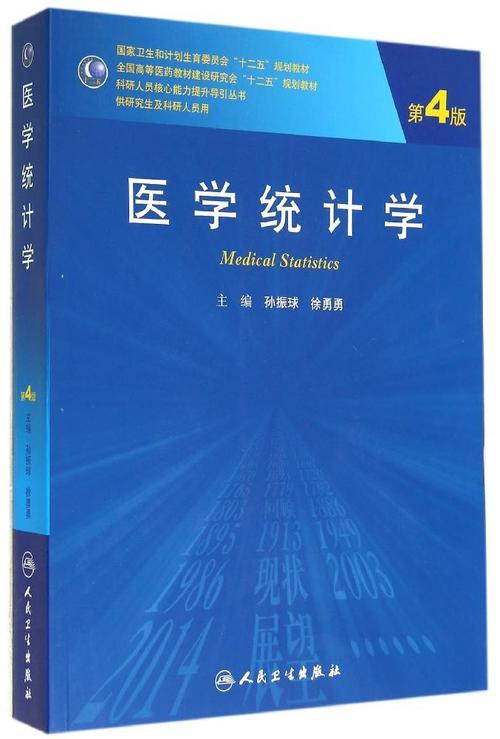
\includegraphics[width=0.25\linewidth]{image/Ms_logo} \end{center}

虽然在学习,整理过程中尽量将笔记的形式,内容结构进行力所能及的梳理,这里要特别感谢在学习过程中,在网络上找到的一些参考资料带来的帮助,然后将一些
示例与原书进行对照,以避免一些学习错误,但个人能力和精力实在有限,也容易会有理解不当,表述错误的情况,
如果您在参考的过程中,发现了这样的错误,请您尽量可以告诉我,我会确认并努力修正,如果您对文档有疑问或建议,都可以 \textbf{\href{mailto:wxh244295043@gamil.com}{邮件}} 告知我。

建议您购买原版教材结合本笔记学习,您也可以在网络上找到电子书方便参考。

形成此文档对我来讲是一个很大的挑战,需要耗费巨大精力。另外,因为本人特殊情况,难以像以前正常工作,所以也是以此方式
保持学习能力,和提升自己。希望这份文档能对您有所助益,如果正是如此,您愿意的话可以捐助我,这里先谢过鼓励和支持的朋友\textasciitilde{}

\begin{center}
\includegraphics[width=0.7\linewidth]{image/SponsorshipFig} \end{center}

\hypertarget{ux8f6fux4ef6ux51c6ux5907}{%
\subsubsection{软件准备}\label{ux8f6fux4ef6ux51c6ux5907}}

本文档使用到的主要软件 \href{https://www.r-project.org/}{R}版本是4.0.3, 和 \href{https://rstudio.com/}{RStudio},版本是 1.3.1093 .

如果您R语言的新手,您可以在下面找到一些快速上手的学习资料:

\begin{enumerate}
\def\labelenumi{\arabic{enumi}.}
\tightlist
\item
  \href{https://rstudio.com/resources/cheatsheets/}{RStudio Cheatsheets}
\item
  \href{https://cran.r-project.org/doc/contrib/Paradis-rdebuts_en.pdf}{R for Beginners}
\end{enumerate}

\begin{Shaded}
\begin{Highlighting}[]
\KeywordTok{sessionInfo}\NormalTok{()}
\CommentTok{## R version 4.0.3 (2020-10-10)}
\CommentTok{## Platform: x86_64-w64-mingw32/x64 (64-bit)}
\CommentTok{## Running under: Windows 10 x64 (build 19041)}
\CommentTok{## Matrix products: default}
\CommentTok{## locale:}
\CommentTok{## [1] LC_COLLATE=Chinese (Simplified)_China.936 }
\CommentTok{## [2] LC_CTYPE=Chinese (Simplified)_China.936   }
\CommentTok{## [3] LC_MONETARY=Chinese (Simplified)_China.936}
\CommentTok{## [4] LC_NUMERIC=C                              }
\CommentTok{## [5] LC_TIME=Chinese (Simplified)_China.936    }
\CommentTok{## attached base packages:}
\CommentTok{## [1] stats     graphics  grDevices utils     datasets  methods   base     }
\CommentTok{## loaded via a namespace (and not attached):}
\CommentTok{##  [1] compiler_4.0.3  bookdown_0.21   htmltools_0.5.0 tools_4.0.3    }
\CommentTok{##  [5] yaml_2.2.1      tinytex_0.27    rmarkdown_2.5   knitr_1.30     }
\CommentTok{##  [9] digest_0.6.27   xfun_0.19       rlang_0.4.8     evaluate_0.14  }
\end{Highlighting}
\end{Shaded}

\hypertarget{ux4f20ux9001ux95e8}{%
\subsection{传送门}\label{ux4f20ux9001ux95e8}}

如果您希望快速找到R处理数据的方法,可以通过下面几张插图里面的传送门进行传送。注意的是,似乎Rmarkdown里面对
SVG插图中包含链接展示无法支持,所以你可以

\begin{enumerate}
\def\labelenumi{\arabic{enumi}.}
\tightlist
\item
  \emph{``右击''}插图,选择在 \emph{``新标签页打开图片''},然后新标页签打开的图片。这样可以找到图片中包含的超链接,快速找到合适的章节内容。
\item
  \emph{``右击''}插图,选择在 \emph{``图片另存为''},这样包含的超链接图片保存下来,可以在需要的时候快速找到合适的章节内容。
\end{enumerate}

\begin{figure}

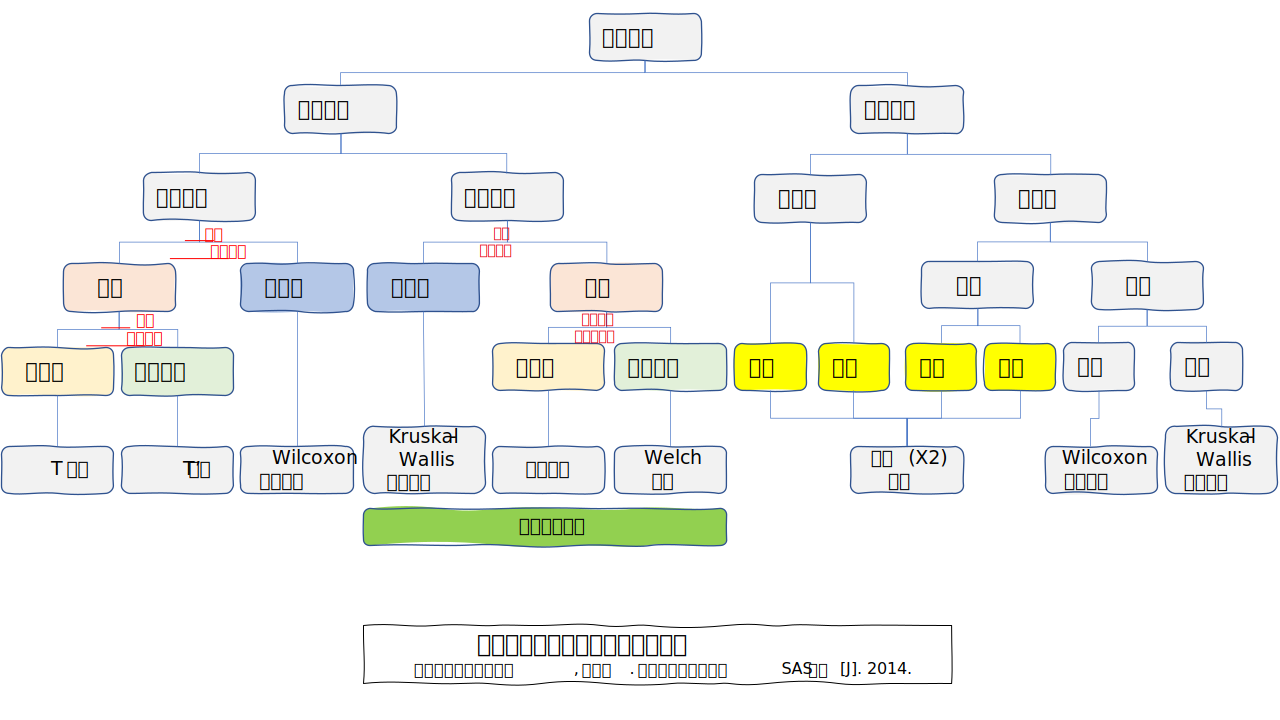
\includegraphics[width=0.9\linewidth]{image/ChoiceStatisticalMethods_href} \hfill{}

\caption{完全随机设计的统计方法选择思路(目前, 传送门还不完整,在随书更新ing)}\label{fig:Gateway1}
\end{figure}

\hypertarget{ux81f4ux8c22}{%
\subsection{致谢}\label{ux81f4ux8c22}}

谨以此书献给我的家人,想在此感谢母亲和父亲,纪念祝愿我的姐姐及她的两个丫头。

最后,祝愿到此一游的你我他! ̄▽ ̄

\hypertarget{ux58f0ux660e}{%
\subsection{声明}\label{ux58f0ux660e}}

本笔记可供选修《医学统计学》课程的同学学习使用,如果您需要将素材和代码作其它用途,请联系作者:\href{mailto:wxh244295043@gmail.com}{\nolinkurl{wxh244295043@gmail.com}}。

\hypertarget{ux7b2cux4e8cux7ae0-ux8ba1ux91cfux8d44ux6599ux7684ux7edfux8ba1ux63cfux8ff0}{%
\section{第二章 计量资料的统计描述}\label{ux7b2cux4e8cux7ae0-ux8ba1ux91cfux8d44ux6599ux7684ux7edfux8ba1ux63cfux8ff0}}

日期: 2020-11-10
作者:wxhyihuan

\hypertarget{ux63cfux8ff0ux7edfux8ba1}{%
\subsection{描述统计}\label{ux63cfux8ff0ux7edfux8ba1}}

描述统计学(广义上的描述统计学,Descriptive statistics)是统计学的一个分支,旨在概括、描述和呈现一系列值或数据集(比如对单样本的分析)。
由于难以识别数据中的任何模式,没有任何准备或没有任何汇总度量的长系列值通常无法提供信息。

描述统计通常是统计分析的第一步,也是统计分析的重要组成部分。它允许通过检测潜在的异常值(即似乎与其他数据分离的数据点)、
收集或编码错误来检查数据的质量。它还有助于``理解''数据,如果表述得当,描述性统计是进一步分析的一个很好的起点。

位置与离散度量是两种不同的总结数据的测量方法。其中一些给出了关于数据位置的理解,另一些给出了关于数据分散性的理解。
在实践中,这两种度量方法经常一起使用,以便以最简洁和完整的方式总结数据。

位置度量允许查看数据位于``何处'',围绕哪个值。换句话说,位置度量可了解什么是总体趋势,即数据整体的``位置''。
它主要包括:\emph{平均值,中位数,四分位数,第三、四分位数,众数,最大值,最小值等}。

常见的离散度量,它有助于了解离散度和数据的可变性(在何种程度上分布被压缩或拉伸):\emph{范围,标准偏差,方差,四分位间距,变异系数}。

\hypertarget{ux6d4bux8bd5ux6570ux636e}{%
\subsection{测试数据}\label{ux6d4bux8bd5ux6570ux636e}}

\begin{table}

\caption{\label{tab:tab1}某医院用随机抽样的方法检测了138名正常成年女子的红细胞数目(RBC, $*10^{12}/L$),其测量结果如下表:}
\centering
\begin{tabular}[t]{cccccccccccc}
\toprule
V1 & V2 & V3 & V4 & V5 & V6 & V7 & V8 & V9 & V10 & V11 & V12\\
\midrule
3.96 & 4.23 & 4.42 & 3.59 & 5.12 & 4.02 & 4.32 & 3.72 & 4.76 & 4.16 & 4.61 & 4.26\\
3.77 & 4.20 & 4.36 & 3.07 & 4.89 & 3.97 & 4.28 & 3.64 & 4.66 & 4.04 & 4.55 & 4.25\\
4.63 & 3.91 & 4.41 & 3.52 & 5.03 & 4.01 & 4.30 & 4.19 & 4.75 & 4.14 & 4.57 & 4.26\\
4.56 & 3.79 & 3.89 & 4.21 & 4.95 & 3.98 & 4.29 & 3.67 & 4.69 & 4.12 & 4.56 & 4.26\\
4.66 & 4.28 & 3.83 & 4.20 & 5.24 & 4.02 & 4.33 & 3.76 & 4.81 & 4.17 & 3.96 & 3.27\\
\addlinespace
4.61 & 4.26 & 3.96 & 4.23 & 3.76 & 4.01 & 4.29 & 3.67 & 3.39 & 4.12 & 4.27 & 3.61\\
4.98 & 4.24 & 3.83 & 4.20 & 3.71 & 4.03 & 4.34 & 4.69 & 3.62 & 4.18 & 4.26 & 4.36\\
5.28 & 4.21 & 4.42 & 4.36 & 3.66 & 4.02 & 4.31 & 4.83 & 3.59 & 3.97 & 3.96 & 4.49\\
5.11 & 4.20 & 4.36 & 4.54 & 3.72 & 3.97 & 4.28 & 4.76 & 3.21 & 4.04 & 4.56 & 4.25\\
4.92 & 4.23 & 4.47 & 3.60 & 5.23 & 4.02 & 4.32 & 4.68 & 4.76 & 3.69 & 4.61 & 4.26\\
\addlinespace
3.89 & 4.21 & 4.36 & 3.42 & 5.01 & 4.01 & 4.29 & 3.68 & 4.71 & 4.13 & 4.57 & 4.26\\
4.03 & 5.46 & 4.16 & 3.64 & 4.16 & 3.76 &  &  &  &  &  & \\
\bottomrule
\end{tabular}
\end{table}

\hypertarget{ux6570ux636eux8f93ux5165ux548cux9891ux7387ux7edfux8ba1}{%
\subsection{数据输入和频率统计}\label{ux6570ux636eux8f93ux5165ux548cux9891ux7387ux7edfux8ba1}}

\hypertarget{ux8bfbux53d6ux6570ux636eux5e76ux5c06ux6570ux636eux8f6cux6362ux6210ux5355ux5217ux5f62ux5f0f}{%
\subsubsection{读取数据,并将数据转换成单列形式}\label{ux8bfbux53d6ux6570ux636eux5e76ux5c06ux6570ux636eux8f6cux6362ux6210ux5355ux5217ux5f62ux5f0f}}

\begin{Shaded}
\begin{Highlighting}[]
\NormalTok{RBC<-}\KeywordTok{read.table}\NormalTok{(}\StringTok{"ExampleData/02-01.txt"}\NormalTok{,}\DataTypeTok{sep=}\StringTok{"}\CharTok{\textbackslash{}t}\StringTok{"}\NormalTok{)}
\NormalTok{RBC<-}\KeywordTok{as.matrix}\NormalTok{(RBC)}
\NormalTok{RBC_q <-}\StringTok{ }\KeywordTok{c}\NormalTok{()}
\ControlFlowTok{for}\NormalTok{ (i }\ControlFlowTok{in} \KeywordTok{seq}\NormalTok{(}\DecValTok{1}\OperatorTok{:}\KeywordTok{nrow}\NormalTok{(RBC)))\{}
\NormalTok{  RBC_q <-}\StringTok{ }\KeywordTok{c}\NormalTok{(RBC_q, RBC[i,])}
\NormalTok{\}}
\NormalTok{RBC_v<-}\KeywordTok{as.vector}\NormalTok{(RBC_q)}
\NormalTok{RBC_v<-}\KeywordTok{na.omit}\NormalTok{(RBC_v)}
\end{Highlighting}
\end{Shaded}

\hypertarget{ux8ba1ux7b97ux6781ux5dee-maxminrange}{%
\subsubsection{计算极差, max()/min()/range()}\label{ux8ba1ux7b97ux6781ux5dee-maxminrange}}

\begin{Shaded}
\begin{Highlighting}[]
\CommentTok{#range(RBC_v)  返回最小值和最大值}
\NormalTok{rge<-}\KeywordTok{max}\NormalTok{(RBC_v)}\OperatorTok{-}\KeywordTok{min}\NormalTok{(RBC_v)}
\NormalTok{rge}
\CommentTok{## [1] 2.39}
\end{Highlighting}
\end{Shaded}

\hypertarget{ux786eux5b9aux7ec4ux6bb5ux6570ux548cux7ec4ux8ddd}{%
\subsubsection{确定组段数和组距}\label{ux786eux5b9aux7ec4ux6bb5ux6570ux548cux7ec4ux8ddd}}

可以参考PAST软件中的the zero-stage rule of Wand 1997方式计算分段``最佳''个数。\(h=3.49min(s,IQ/1.349)n^{1/3}\),其中s是样本标准差,IQ是四分位数范围。

\begin{Shaded}
\begin{Highlighting}[]
\CommentTok{#sd()计算标准差,quantile()计算分位数}
\NormalTok{s<-}\KeywordTok{sd}\NormalTok{(RBC_v)}
\CommentTok{## [1] 0.4457298}
\NormalTok{quan<-}\KeywordTok{quantile}\NormalTok{(RBC_v,}\KeywordTok{c}\NormalTok{(}\FloatTok{0.25}\NormalTok{,}\FloatTok{0.75}\NormalTok{))}
\NormalTok{iq<-quan[}\DecValTok{2}\NormalTok{]}\OperatorTok{-}\NormalTok{quan[}\DecValTok{1}\NormalTok{]}
\CommentTok{## 0.565}
\NormalTok{h<-}\FloatTok{3.49}\OperatorTok{*}\KeywordTok{min}\NormalTok{(s,iq}\OperatorTok{/}\FloatTok{1.349}\NormalTok{)}\OperatorTok{*}\NormalTok{(}\KeywordTok{length}\NormalTok{(RBC_v)}\OperatorTok{^}\NormalTok{(}\DecValTok{1}\OperatorTok{/}\DecValTok{3}\NormalTok{))}
\CommentTok{## 7.553617}
\NormalTok{h<-}\KeywordTok{ceiling}\NormalTok{(h)}
\CommentTok{## 8}
\NormalTok{i<-rge}\OperatorTok{/}\NormalTok{h}
\end{Highlighting}
\end{Shaded}

\hypertarget{ux8ba1ux7b97ux9891ux6570ux5206ux5e03}{%
\subsubsection{计算频数分布}\label{ux8ba1ux7b97ux9891ux6570ux5206ux5e03}}

根据计算的短组段数(h=8),极差值(rge=2.39))和组距(i=rge/h=0.3164)计算各组段的频数。

\begin{Shaded}
\begin{Highlighting}[]
\NormalTok{breaks =}\StringTok{ }\KeywordTok{seq}\NormalTok{(}\KeywordTok{min}\NormalTok{(RBC_v), }\KeywordTok{max}\NormalTok{(RBC_v), }\DataTypeTok{length.out =} \DecValTok{8}\NormalTok{)}
\NormalTok{RBC_v.cut =}\StringTok{ }\KeywordTok{cut}\NormalTok{(RBC_v, breaks, }\DataTypeTok{right=}\NormalTok{T,}\DataTypeTok{include.lowest=}\NormalTok{T)}
\NormalTok{RBC_v.freq =}\StringTok{ }\KeywordTok{table}\NormalTok{(RBC_v.cut)}
\CommentTok{## [3.07,3.41) [3.41,3.75) [3.75,4.09) [4.09,4.44) [4.44,4.78) }
\CommentTok{##          4          17          29          51          23 }
\CommentTok{## [4.78,5.12) [5.12,5.46) }
\CommentTok{##          9           4 }
\KeywordTok{hist}\NormalTok{(RBC_v, }\DataTypeTok{right=}\OtherTok{FALSE}\NormalTok{, }
     \DataTypeTok{breaks =}\NormalTok{ breaks, }\DataTypeTok{labels =}\OtherTok{TRUE}\NormalTok{, }
     \DataTypeTok{freq =} \OtherTok{TRUE}\NormalTok{, }\DataTypeTok{col =} \StringTok{"#A8D6FF"}\NormalTok{, }
     \DataTypeTok{border =} \StringTok{"white"}\NormalTok{, }\DataTypeTok{ylim=}\KeywordTok{c}\NormalTok{(}\DecValTok{0}\NormalTok{, }\KeywordTok{max}\NormalTok{(RBC_v.freq))) }

\KeywordTok{hist}\NormalTok{(RBC_v, }\DataTypeTok{right=}\OtherTok{FALSE}\NormalTok{, }
      \DataTypeTok{breaks =}\NormalTok{ breaks, }\DataTypeTok{labels =}\OtherTok{TRUE}\NormalTok{, }
      \DataTypeTok{freq =} \OtherTok{FALSE}\NormalTok{, }\DataTypeTok{col =} \StringTok{"#A8D6FF"}\NormalTok{, }
      \DataTypeTok{border =} \StringTok{"white"}\NormalTok{, }\DataTypeTok{ylim=}\KeywordTok{c}\NormalTok{(}\DecValTok{0}\NormalTok{,}\DecValTok{1}\NormalTok{))}
\KeywordTok{lines}\NormalTok{(}\KeywordTok{density}\NormalTok{(RBC_v),}\DataTypeTok{col=}\StringTok{"red"}\NormalTok{,}\DataTypeTok{lwd=}\DecValTok{2}\NormalTok{)}
\end{Highlighting}
\end{Shaded}

\begin{figure}

{\centering 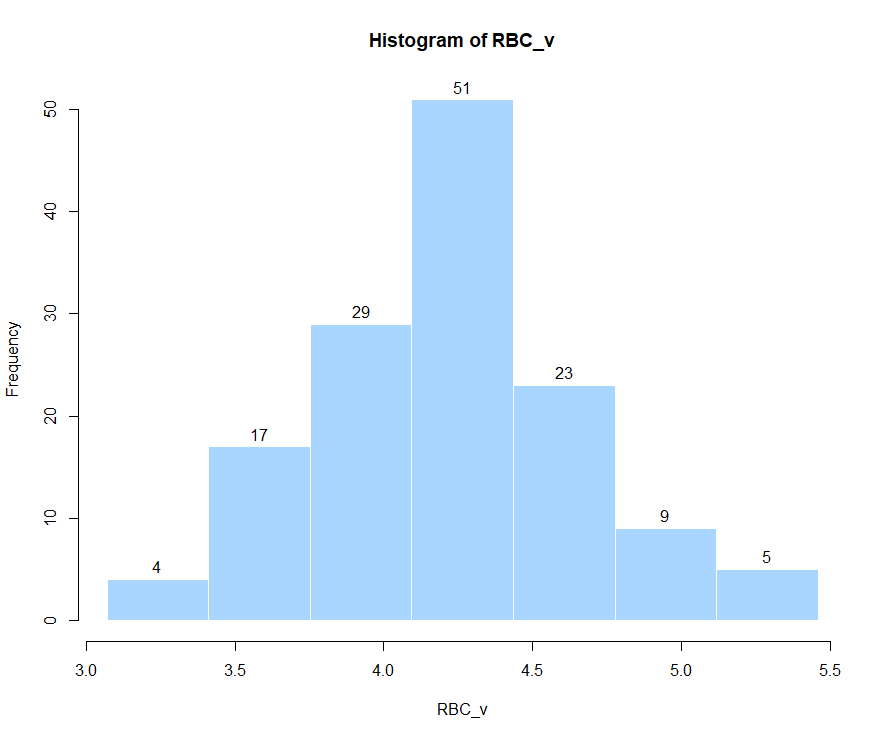
\includegraphics[width=0.49\linewidth,height=0.49\textheight]{image/a1e3904af844b14d3b57d1448690aea} 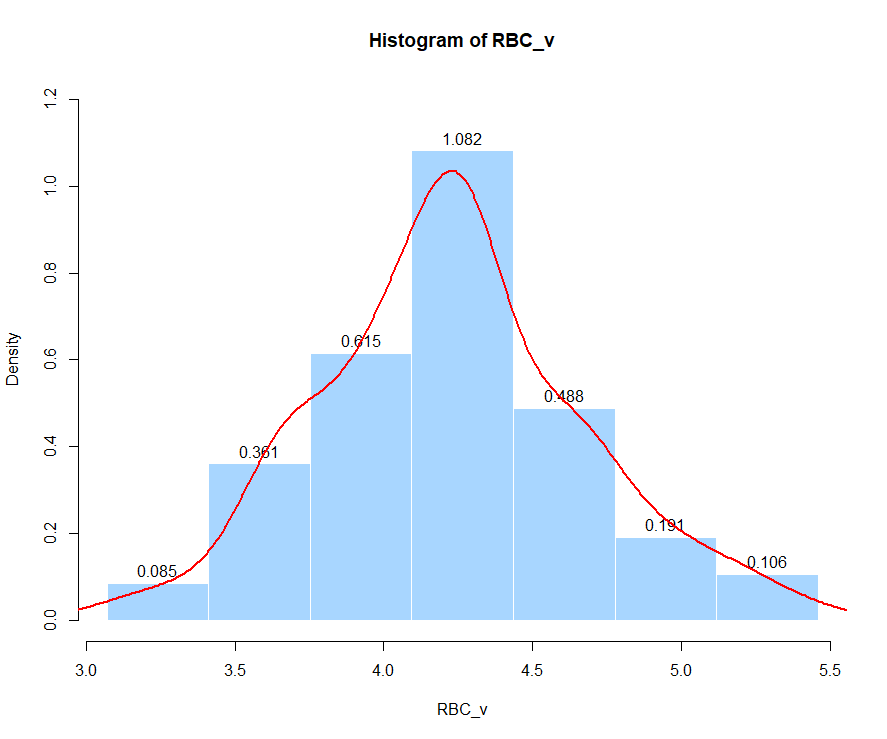
\includegraphics[width=0.49\linewidth,height=0.49\textheight]{image/5ba23e818daa7c71b147707f9b5dfd6} 

}

\caption{红细胞含量的频数分布}\label{fig:histgrah}
\end{figure}

\hypertarget{ux63cfux8ff0ux6027ux7edfux8ba1ux7684ux5ea6ux91cf}{%
\subsection{描述性统计的度量}\label{ux63cfux8ff0ux6027ux7edfux8ba1ux7684ux5ea6ux91cf}}

\hypertarget{ux7b97ux672fux5e73ux5747ux503c}{%
\subsubsection{算术平均值}\label{ux7b97ux672fux5e73ux5747ux503c}}

算术均数简称均值(mean),用于反映组呈对称分布的变量值在数量上的平均水平。

\begin{Shaded}
\begin{Highlighting}[]
\KeywordTok{mean}\NormalTok{(RBC_v)}
\CommentTok{## [1] 4.227029}
\end{Highlighting}
\end{Shaded}

\hypertarget{ux51e0ux4f55ux5e73ux5747ux503c}{%
\subsubsection{几何平均值}\label{ux51e0ux4f55ux5e73ux5747ux503c}}

几何均数(geometric mean)可用于反映一组经 \textbf{对数转换} 后呈对称分布的变量值在数量上的平均水平。

\begin{Shaded}
\begin{Highlighting}[]
\KeywordTok{exp}\NormalTok{(}\KeywordTok{mean}\NormalTok{(}\KeywordTok{log}\NormalTok{(RBC_v)))}
\CommentTok{## [1] 4.203676}
\end{Highlighting}
\end{Shaded}

\hypertarget{ux4e2dux4f4dux6570ux4e0eux767eux5206ux4f4dux6570}{%
\subsubsection{中位数与百分位数}\label{ux4e2dux4f4dux6570ux4e0eux767eux5206ux4f4dux6570}}

中位数(median)是将n个变量值从小到大排列,位置居于中间的那个数。当为奇数时取位次居中 的变量值,当n为偶数时取位次居中的两个变量值的均数。
它适用于各种分布类型的资料,尤其是偏态分 布资料和一端或两端无确切数值的资料。

\begin{Shaded}
\begin{Highlighting}[]
\CommentTok{#中位数(=50百分位)}
\KeywordTok{median}\NormalTok{(RBC_v)}
\KeywordTok{quantile}\NormalTok{(RBC_v,  }\FloatTok{0.5}\NormalTok{)}
\CommentTok{##  4.23}
\CommentTok{#百分位}
\KeywordTok{quantile}\NormalTok{(RBC_v, }\KeywordTok{c}\NormalTok{(}\FloatTok{0.1}\NormalTok{, }\FloatTok{0.25}\NormalTok{, }\FloatTok{0.5}\NormalTok{,}\FloatTok{0.75}\NormalTok{,}\FloatTok{0.9}\NormalTok{))}
\CommentTok{##    10%    25%    50%    75%    90% }
\CommentTok{##3.6670 3.9625 4.2300 4.5275 4.7750 }
\end{Highlighting}
\end{Shaded}

\hypertarget{ux6781ux5dee}{%
\subsubsection{极差}\label{ux6781ux5dee}}

极差即一组变量值的最大值与最小值之差。

\begin{Shaded}
\begin{Highlighting}[]
\KeywordTok{max}\NormalTok{(RBC_v)}\OperatorTok{-}\KeywordTok{min}\NormalTok{(RBC_v)}
\KeywordTok{range}\NormalTok{(RBC_v)}
\end{Highlighting}
\end{Shaded}

\hypertarget{ux56dbux5206ux4f4dux95f4ux8ddd}{%
\subsubsection{四分位间距}\label{ux56dbux5206ux4f4dux95f4ux8ddd}}

四分位数(quartile)是把全部变量值分为四部分的分位数,即第1四分位数(Q .=Ps)、第2四分位数 M=P)、第3四分位数 (Qu=Ps)。 四分位数间距(quartile range)是由第3四分位数和第1四分位数相减行得,
记为 R.它般和中位数起描述偏态分们资料的分布特征

\begin{Shaded}
\begin{Highlighting}[]
\CommentTok{#四分位间距interquartile range}
\KeywordTok{IQR}\NormalTok{(RBC_v)}
\CommentTok{##  0.565}
\KeywordTok{quantile}\NormalTok{(RBC_v, }\FloatTok{0.75}\NormalTok{)}\OperatorTok{-}\KeywordTok{quantile}\NormalTok{(RBC_v, }\FloatTok{0.25}\NormalTok{)}
\CommentTok{## 0.565}
\end{Highlighting}
\end{Shaded}

\hypertarget{ux65b9ux5deeux4e0eux6807ux51c6ux5dee}{%
\subsubsection{方差与标准差}\label{ux65b9ux5deeux4e0eux6807ux51c6ux5dee}}

方差(variance,var)也称均方差(mean Square deviation),反映一组数据的平均离散水平。
标准差(standard deviation,sd)是方差的正平方根,其单位与原变量值的单位相同。

\begin{Shaded}
\begin{Highlighting}[]
\CommentTok{#计算标准差}
\KeywordTok{sd}\NormalTok{(RBC_v)}
\CommentTok{## [1] 0.4457298}
\CommentTok{#计算方差}
\KeywordTok{var}\NormalTok{(RBC_v)}
\CommentTok{## [1] 0.1986751}
\KeywordTok{sd}\NormalTok{(RBC_v)}\OperatorTok{^}\DecValTok{2}
\NormalTok{(}\KeywordTok{sum}\NormalTok{((RBC_v}\OperatorTok{-}\KeywordTok{mean}\NormalTok{(RBC_v))}\OperatorTok{^}\DecValTok{2}\NormalTok{))}\OperatorTok{/}\NormalTok{(}\KeywordTok{length}\NormalTok{(RBC_v)}\OperatorTok{-}\DecValTok{1}\NormalTok{)}
\CommentTok{## 0.1986751}
\end{Highlighting}
\end{Shaded}

\hypertarget{ux53d8ux5f02ux7cfbux6570}{%
\subsubsection{变异系数}\label{ux53d8ux5f02ux7cfbux6570}}

变异系数(Cefficient of variation,CV),当进行两个或多个资料变异程度的比较时,如果度量单位与平均数相同,
可以直接利用标准差来比较。如果单位和(或)平均数不同时,比较其变异程度就不能采用标准差,
而需采用标准差与平均数的比值(相对值)来比较。标准差与平均数的比值称为变异系数,。
变异系数可以消除单位和(或)平均数不同对两个或多个资料变异程度比较的影响。

\begin{Shaded}
\begin{Highlighting}[]
\KeywordTok{sd}\NormalTok{(RBC_v)}\OperatorTok{/}\KeywordTok{mean}\NormalTok{(RBC_v)}\OperatorTok{*}\DecValTok{100}
\CommentTok{## [1] 10.54475}
\NormalTok{raster}\OperatorTok{::}\KeywordTok{cv}\NormalTok{(RBC_v)}
\CommentTok{## [1] 10.54475}
\end{Highlighting}
\end{Shaded}

\hypertarget{ux5176ux4ed6ux7684ux63cfux8ff0ux7edfux8ba1}{%
\subsubsection{其他的描述统计}\label{ux5176ux4ed6ux7684ux63cfux8ff0ux7edfux8ba1}}

\hypertarget{summary}{%
\paragraph{Summary}\label{summary}}

R语言中,可以使用summary()来计算最小,第1四分位数,中位数,平均值,第3,4分位数和最大值的数据集的所有数值变量。

\begin{Shaded}
\begin{Highlighting}[]
\NormalTok{dat <-}\StringTok{ }\NormalTok{iris}
\KeywordTok{summary}\NormalTok{(dat)}
\CommentTok{##  Sepal.Length    Sepal.Width     Petal.Length    Petal.Width          Species  }
\CommentTok{## Min.   :4.300   Min.   :2.000   Min.   :1.000   Min.   :0.100   setosa    :50  }
\CommentTok{## 1st Qu.:5.100   1st Qu.:2.800   1st Qu.:1.600   1st Qu.:0.300   versicolor:50  }
\CommentTok{## Median :5.800   Median :3.000   Median :4.350   Median :1.300   virginica :50  }
\CommentTok{## Mean   :5.843   Mean   :3.057   Mean   :3.758   Mean   :1.199                  }
\CommentTok{## 3rd Qu.:6.400   3rd Qu.:3.300   3rd Qu.:5.100   3rd Qu.:1.800                  }
\CommentTok{## Max.   :7.900   Max.   :4.400   Max.   :6.900   Max.   :2.500                  }
\end{Highlighting}
\end{Shaded}

\hypertarget{ux4f17ux6570}{%
\paragraph{众数}\label{ux4f17ux6570}}

众数(Mode)是指在统计分布上具有明显集中趋势点的数值,代表数据的一般水平。 也是一组数据中出现次数最多的数值,有时众数在一组数中有好几个。
可以利用table()和sort()来寻找数据集中的众数。

\begin{Shaded}
\begin{Highlighting}[]
\CommentTok{# 计算每个元素的出现的次数}
\NormalTok{RBC_t <-}\StringTok{ }\KeywordTok{table}\NormalTok{(RBC_v) }
 \CommentTok{# 对计算的次数进行排序}
\KeywordTok{sort}\NormalTok{(RBC_t, }\DataTypeTok{decreasing =} \OtherTok{TRUE}\NormalTok{) }
\CommentTok{##  4.26 4.36 3.96 4.02  4.2 3.76 3.97 4.01 4.16 4.21 4.23 4.28 4.29 4.56 4.61 4.76 }
\CommentTok{##     7    5    4    4    4    3    3    3    3    3    3    3    3    3    3    3 }
\CommentTok{##  3.59 3.64 3.67 3.72 3.83 3.89 4.03 4.04 4.12 4.25 4.32 4.42 4.57 4.66 4.69 3.07 }
\CommentTok{##     2    2    2    2    2    2    2    2    2    2    2    2    2    2    2    1 }
\CommentTok{##  3.21 3.27 3.39 3.42 3.52  3.6 3.61 3.62 3.66 3.68 3.69 3.71 3.77 3.79 3.91 3.98 }
\CommentTok{##     1    1    1    1    1    1    1    1    1    1    1    1    1    1    1    1 }
\CommentTok{##  4.13 4.14 4.17 4.18 4.19 4.24 4.27  4.3 4.31 4.33 4.34 4.41 4.47 4.49 4.54 4.55 }
\CommentTok{##     1    1    1    1    1    1    1    1    1    1    1    1    1    1    1    1 }
\CommentTok{##  4.63 4.68 4.71 4.75 4.81 4.83 4.89 4.92 4.95 4.98 5.01 5.03 5.11 5.12 5.23 5.24 }
\CommentTok{##     1    1    1    1    1    1    1    1    1    1    1    1    1    1    1    1 }
\CommentTok{##  5.28 5.46 }
\CommentTok{##     1    1 }

\CommentTok{#或者结合 which()函数确定众数和其次数}
\NormalTok{RBC_t[}\KeywordTok{which}\NormalTok{(((RBC_t}\OperatorTok{==}\KeywordTok{max}\NormalTok{(RBC_t))}\OperatorTok{==}\NormalTok{T))]}
\CommentTok{## 4.26 }
\CommentTok{##    7 }
\end{Highlighting}
\end{Shaded}

\hypertarget{ux6b63ux6001ux5206ux5e03ux548cux6807ux51c6ux6b63ux6001ux5206ux5e03}{%
\subsection{正态分布和标准正态分布}\label{ux6b63ux6001ux5206ux5e03ux548cux6807ux51c6ux6b63ux6001ux5206ux5e03}}

\href{https://zh.wikipedia.org/zh-cn/\%E6\%AD\%A3\%E6\%80\%81\%E5\%88\%86\%E5\%B8\%83}{正态分布}(Normal distribution)又名高斯分布(Gaussian distribution),是一个非常常见的连续概率分布。
\textbf{正态分布}在统计学上十分重要,经常用在自然和社会科学来代表一个不明的随机变量。
可以说,弄懂正态分布是灵活运用统计学中各种假设检验方法、理解p值,均数置信区间的前提。
R包含有很丰富的正态分布相关的\href{https://stat.ethz.ch/R-manual/R-devel/library/stats/html/Normal.html}{函数功能},
比如概率密度函数dnorm(),概率累积分布函数pnorm(),正态分位函数qnorm()和用来生成特定正态分布数据序列的函数rnorm(),
以及检测数据时候符合正态分布的方法,这里主要做下面一些介绍。

\hypertarget{ux6982ux7387ux5bc6ux5ea6ux51fdux6570dnorm}{%
\subsubsection{概率密度函数dnorm()}\label{ux6982ux7387ux5bc6ux5ea6ux51fdux6570dnorm}}

\href{https://zh.wikipedia.org/zh-cn/\%E6\%A9\%9F\%E7\%8E\%87\%E5\%AF\%86\%E5\%BA\%A6\%E5\%87\%BD\%E6\%95\%B8}{概率密度函数(Probability density function)},R中即为dnorm(),
它可以给出了指定均值和标准差下每个点的\textbf{概率分布的高度},
越高就代表着这个点/区间的概率越密集(大)。概率密度函数有时也被称为概率分布函数,但这种称法可能会和累积分布函数pnorm()混淆。

\begin{Shaded}
\begin{Highlighting}[]
\CommentTok{#在-10~10区间等分的 100个 数据集x}
\NormalTok{x <-}\StringTok{ }\KeywordTok{seq}\NormalTok{(}\OperatorTok{-}\DecValTok{10}\NormalTok{, }\DecValTok{10}\NormalTok{, }\DataTypeTok{by =} \FloatTok{.1}\NormalTok{)}
\CommentTok{#创建一个均值是2.5,标准差是0.5正态分布 y}
\NormalTok{y <-}\StringTok{ }\KeywordTok{dnorm}\NormalTok{(x, }\DataTypeTok{mean =} \FloatTok{2.5}\NormalTok{, }\DataTypeTok{sd =} \FloatTok{0.5}\NormalTok{)}
\CommentTok{#将 y 中的落在x数据集上的数据画出来}
\KeywordTok{plot}\NormalTok{(x,y,}\DataTypeTok{col=}\StringTok{"red"}\NormalTok{,}\DataTypeTok{pch=}\DecValTok{20}\NormalTok{)}
\end{Highlighting}
\end{Shaded}

\begin{figure}

{\centering 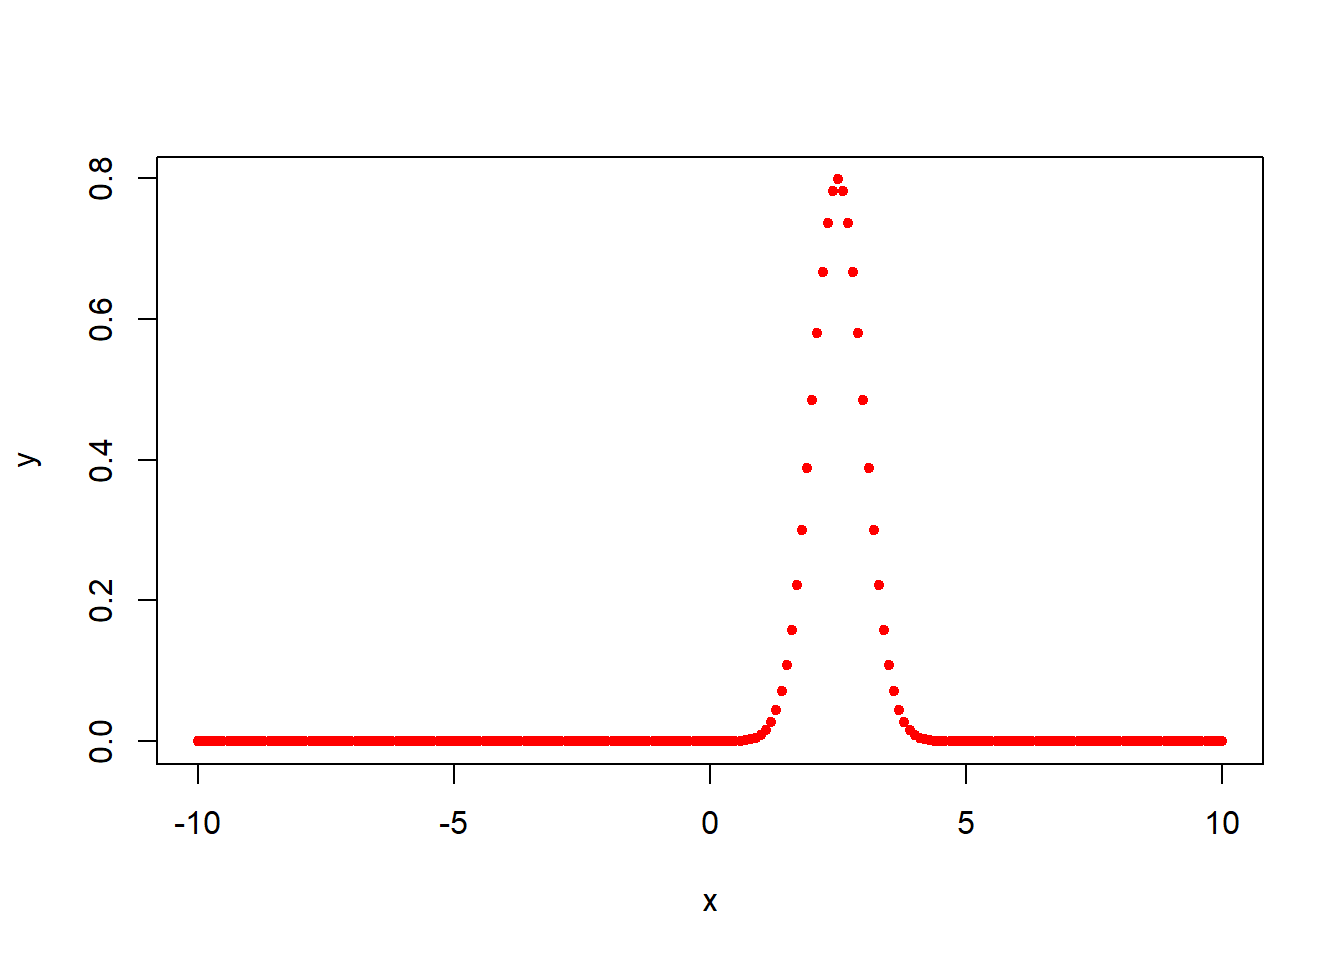
\includegraphics[width=0.49\linewidth,height=0.49\textheight]{figs/dnorm} 

}

\caption{概率密度函数示例}\label{fig:dnorm}
\end{figure}

\hypertarget{ux6982ux7387ux7d2fux79efux5206ux5e03ux51fdux6570pnorm}{%
\subsubsection{概率累积分布函数pnorm()}\label{ux6982ux7387ux7d2fux79efux5206ux5e03ux51fdux6570pnorm}}

\href{https://zh.wikipedia.org/wiki/\%E7\%B4\%AF\%E7\%A7\%AF\%E5\%88\%86\%E5\%B8\%83\%E5\%87\%BD\%E6\%95\%B0}{累积分布函数(Cumulative Distribution Function)},R中即为pnorm(),
又叫分布函数,是概率密度函数的积分,能完整描述一个实随机变量X的概率分布,它给出一个正态分布中小于一个给定数字的累计概率(即指定定点的左边范围的曲线面积)。

\begin{Shaded}
\begin{Highlighting}[]
\CommentTok{#在-10~10区间等分的 40个 数据集x}
\NormalTok{x <-}\StringTok{ }\KeywordTok{seq}\NormalTok{(}\OperatorTok{-}\DecValTok{10}\NormalTok{, }\DecValTok{10}\NormalTok{, }\DataTypeTok{by =} \FloatTok{.5}\NormalTok{)}
\CommentTok{#创建一个均值是2.5,标准差是0.5正态分布 y}
\NormalTok{y <-}\StringTok{ }\KeywordTok{pnorm}\NormalTok{(x, }\DataTypeTok{mean =} \FloatTok{2.5}\NormalTok{, }\DataTypeTok{sd =} \FloatTok{0.5}\NormalTok{)}
\CommentTok{#将 y 中的落在x数据集上的累计概率画出来}
\KeywordTok{plot}\NormalTok{(x,y,}\DataTypeTok{col=}\StringTok{"red"}\NormalTok{,}\DataTypeTok{pch=}\DecValTok{20}\NormalTok{)}
\end{Highlighting}
\end{Shaded}

\begin{figure}

{\centering 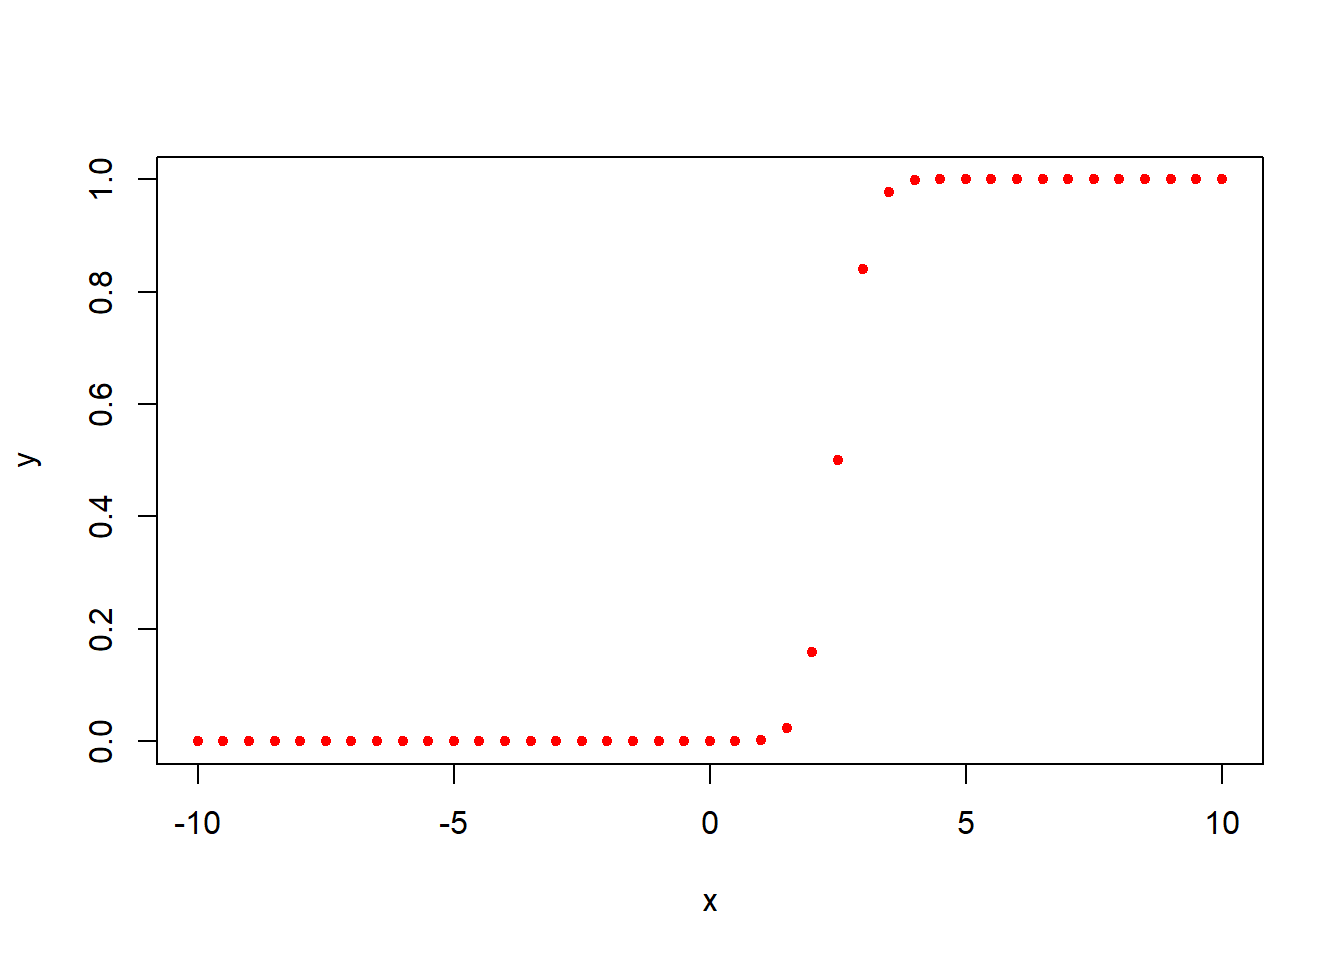
\includegraphics[width=0.49\linewidth,height=0.49\textheight]{figs/pnorm} 

}

\caption{累积分布函数示例}\label{fig:pnorm}
\end{figure}

\hypertarget{ux6b63ux6001ux5206ux4f4dux51fdux6570qnorm}{%
\subsubsection{正态分位函数qnorm()}\label{ux6b63ux6001ux5206ux4f4dux51fdux6570qnorm}}

正态分位函数,R中即为qnorm(),它可以给出一个累积分布概率达到指定值的数字。

\begin{Shaded}
\begin{Highlighting}[]
\CommentTok{#在0~1区间等分的 50个 数据集x}
\NormalTok{x <-}\StringTok{ }\NormalTok{x <-}\StringTok{ }\KeywordTok{seq}\NormalTok{(}\DecValTok{0}\NormalTok{, }\DecValTok{1}\NormalTok{, }\DataTypeTok{by =} \FloatTok{0.02}\NormalTok{)}
\CommentTok{#创建一个均值是2,标准差是1正态分布 y}
\NormalTok{y <-}\StringTok{ }\KeywordTok{qnorm}\NormalTok{(x, }\DataTypeTok{mean =} \DecValTok{2}\NormalTok{, }\DataTypeTok{sd =} \DecValTok{1}\NormalTok{)}
\CommentTok{#将 y 中的落在x数据集上的数字画出来}
\KeywordTok{plot}\NormalTok{(x,y,}\DataTypeTok{col=}\StringTok{"red"}\NormalTok{,}\DataTypeTok{pch=}\DecValTok{20}\NormalTok{)}
\end{Highlighting}
\end{Shaded}

\begin{figure}

{\centering 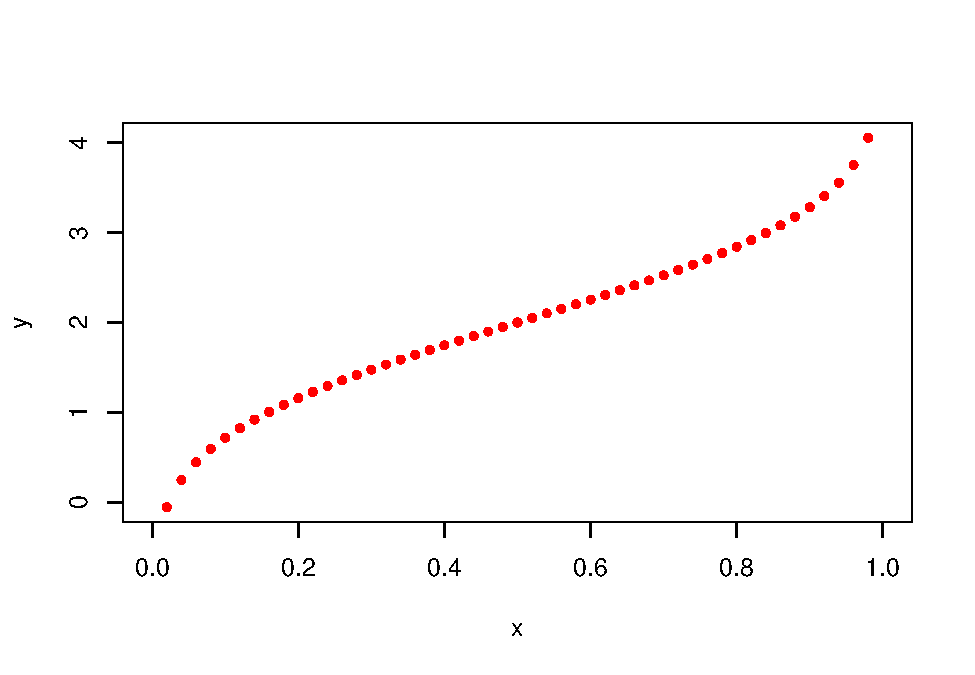
\includegraphics[width=0.49\linewidth,height=0.49\textheight]{figs/qnorm} 

}

\caption{正态分位函数示例}\label{fig:qnorm}
\end{figure}

\hypertarget{ux751fux6210ux6b63ux6001ux5206ux5e03ux51fdux6570rnorm}{%
\subsubsection{生成正态分布函数rnorm()}\label{ux751fux6210ux6b63ux6001ux5206ux5e03ux51fdux6570rnorm}}

rnorm()函数用于生成符合指定均值和标准差的分布为正态分布的随机数,默认是标准正态分布,即均值为0,标准差1的正态分布。

\begin{Shaded}
\begin{Highlighting}[]
\CommentTok{#设置随机种子,便于重复后续的数据选取}
\KeywordTok{set.seed}\NormalTok{(}\DecValTok{50}\NormalTok{)}
\CommentTok{#在标准正态分布中随机选取50个数据}
\NormalTok{y <-}\StringTok{ }\KeywordTok{rnorm}\NormalTok{(}\DecValTok{50}\NormalTok{)}
\CommentTok{#对选区的数据绘制频率分布图}
\KeywordTok{hist}\NormalTok{(y,}\DataTypeTok{col=}\StringTok{"#A8D6FF"}\NormalTok{,}\DataTypeTok{labels =}\OtherTok{TRUE}\NormalTok{)}
\end{Highlighting}
\end{Shaded}

\begin{figure}

{\centering 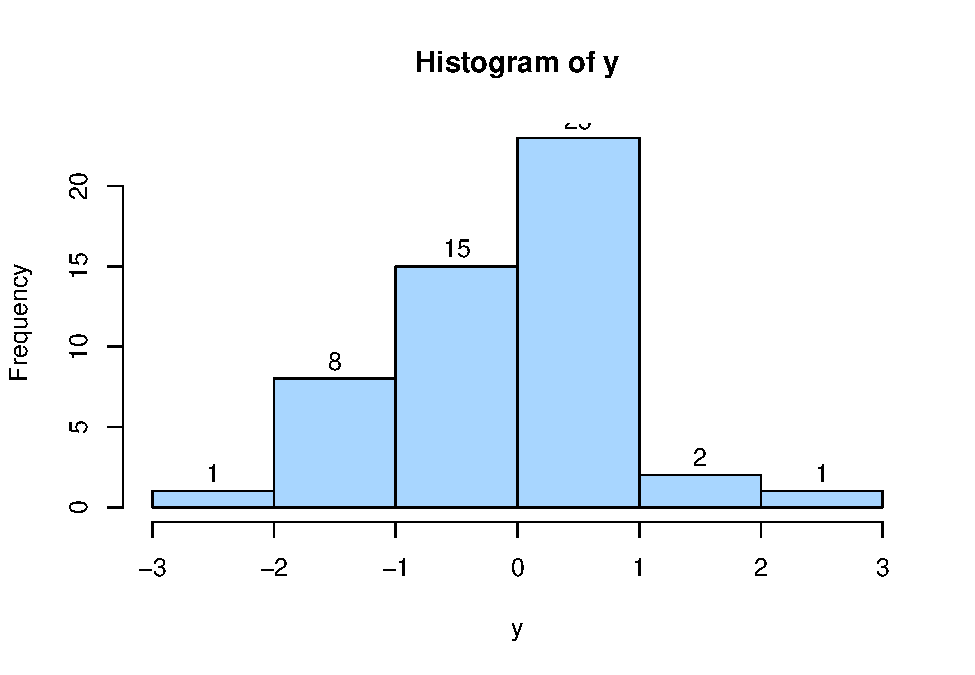
\includegraphics[width=0.49\linewidth,height=0.49\textheight]{figs/rnorm} 

}

\caption{随机正态分布数据示例}\label{fig:rnorm}
\end{figure}

\hypertarget{ux6b63ux6001ux5206ux5e03ux68c0ux9a8c}{%
\subsection{正态分布检验}\label{ux6b63ux6001ux5206ux5e03ux68c0ux9a8c}}

许多计量资料的分析方法要求数据分布是正态或近似正态,因此对原始独立测定数据进行正态性检验是十分必要的。通过绘制数据的频数分布直方图来定性地判断数据分布正态性。

以下正态检验的资料整理自:

\begin{enumerate}
\def\labelenumi{\arabic{enumi}.}
\item
  \href{https://blog.csdn.net/u013524655/article/details/41053105?utm_medium=distribute.pc_relevant.none-task-blog-baidulandingword-7\&spm=1001.2101.3001.4242}{用R语言做正态分布检验}
\item
  \href{https://www.statsandr.com/blog/do-my-data-follow-a-normal-distribution-a-note-on-the-most-widely-used-distribution-and-how-to-test-for-normality-in-r/}{How to test the normality assumption}
\end{enumerate}

正态性检验主要有三类方法:

\begin{enumerate}
\def\labelenumi{\arabic{enumi}.}
\item
  计算综合统计量
  如动差法、夏皮罗-威尔克Shapiro-Wilk 法(W 检验) 、达戈斯提诺D′Agostino 法(D 检验) 、Shapiro-Francia 法(W′检验)。
\item
  正态分布的拟合优度检验

  如皮尔逊χ2 检验 、对数似然比检验 、柯尔莫哥洛夫Kolmogorov-Smirov 法检验。
\item
  图示法(正态概率图Normal Probability plot)

  如分位数图(Quantile Quantileplot ,简称QQ 图) 、百分位数(Percent Percent plot ,简称PP 图) 和稳定化概率图(Stablized Probability plot ,
  简称SP 图) 等。
\end{enumerate}

统计软件中常用的正态性检验方法

\begin{enumerate}
\def\labelenumi{\arabic{enumi}.}
\item
  用偏态系数和峰态系数检验数据正态性

  偏态系数Sk,它用于检验不对称性;峰态系数Ku,它用于检验峰态。 S k= 0, K u= 0 时, 分布呈正态, S k\textgreater{} 0 时, 分布呈正偏态,S k \textless{} 0 时, 分布呈负偏态。适用条件:样本含量应大于200
\item
  用夏皮罗-威尔克(Shapiro-Wilk)法检验数据正态性
  即W检验,1965 年提出,适用于样本含量n ≤50 时的正态性检;。
\item
  用达戈斯提诺(D′Agostino)法检验数据正态性
  即D检验,1971提出,正态性D检验该方法效率高,是比较精确的正态检验法。
\item
  Shapiro-Francia 法
  即W′检验,于1972 年提出,适用于50 \textless{} n \textless{} 100 时的正态性检验。
\item
  QQ图或PP图
  散点聚集在固定直线的周围,可以认为数据资料近似服从正态分布
\end{enumerate}

\textbf{常用的规则}:

\textbf{SPSS 规定}:当样本含量3 ≤n ≤5000 时,结果以Shapiro - Wilk (W 检验) 为难,当样本含量n \textgreater{} 5000 结果以Kolmogorov - Smirnov 为准。

\textbf{SAS 规定}:当样本含量n ≤2000 时,结果以Shapiro - Wilk (W 检验) 为准,当样本含量n \textgreater2000 时,结果以Kolmogorov - Smirnov (D 检验) 为准。

参考:

刘庆武,胡志艳,如何用SPSS、SAS 统计软件进行正态性检验,湘南学院学报(自然科学版),2005
朱红兵,何丽娟,在SPSS10.0 中进行数据资料正态性检验的方法,首都体育学院学报,2004

\hypertarget{ux76f4ux65b9ux56fe}{%
\subsubsection{直方图}\label{ux76f4ux65b9ux56fe}}

直方图显示了分布的分布范围和形状,因此它是评估正态性的一个很好的起点。本文开始测试的红细胞浓度遵循正态曲线,因此数据似乎遵循正态分布。

\begin{Shaded}
\begin{Highlighting}[]
\KeywordTok{hist}\NormalTok{(RBC_v, }\DataTypeTok{right=}\OtherTok{FALSE}\NormalTok{, }
      \DataTypeTok{breaks =}\NormalTok{ breaks, }\DataTypeTok{labels =}\OtherTok{TRUE}\NormalTok{, }
      \DataTypeTok{freq =} \OtherTok{FALSE}\NormalTok{, }\DataTypeTok{col =} \StringTok{"#A8D6FF"}\NormalTok{, }
      \DataTypeTok{border =} \StringTok{"white"}\NormalTok{, }\DataTypeTok{ylim=}\KeywordTok{c}\NormalTok{(}\DecValTok{0}\NormalTok{,}\DecValTok{1}\NormalTok{))}

\KeywordTok{lines}\NormalTok{(}\KeywordTok{density}\NormalTok{(RBC_v),}\DataTypeTok{col=}\StringTok{"red"}\NormalTok{,}\DataTypeTok{lwd=}\DecValTok{2}\NormalTok{)}
\end{Highlighting}
\end{Shaded}

\begin{figure}

{\centering 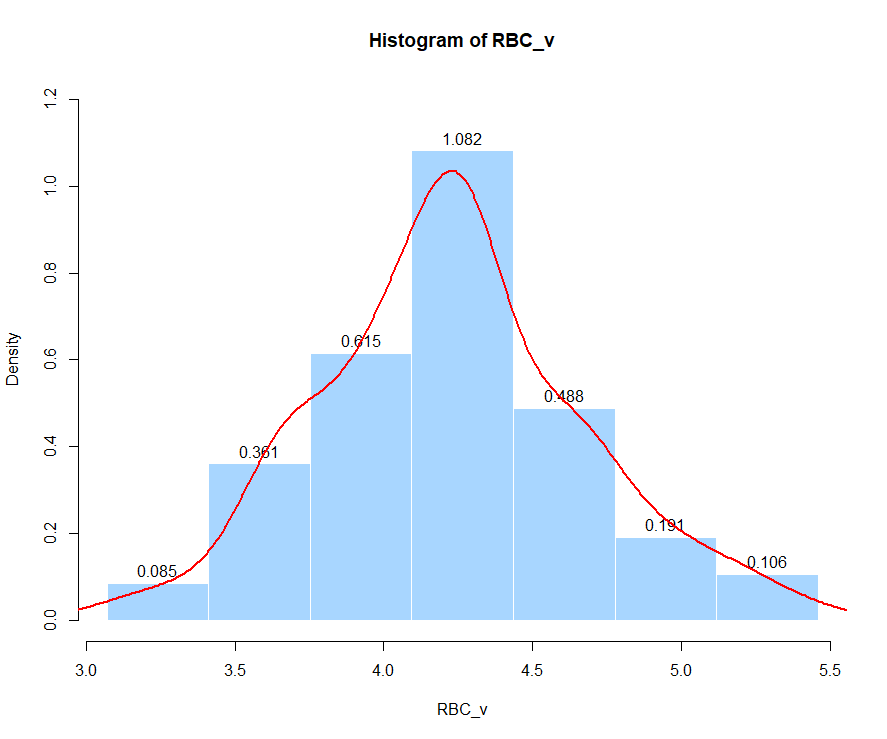
\includegraphics[width=0.49\linewidth,height=0.49\textheight]{image/5ba23e818daa7c71b147707f9b5dfd6} 

}

\caption{正态分布检验与直方图}\label{fig:histtest}
\end{figure}

\hypertarget{ux6982ux7387ux5bc6ux5ea6ux56fe}{%
\subsubsection{概率密度图}\label{ux6982ux7387ux5bc6ux5ea6ux56fe}}

概率密度图图提供了关于数据是否服从正态分布的直观判断。它们类似于直方图,因为它们也允许分析分布的传播和形状。但是,它们是直方图的平滑版本。

\begin{Shaded}
\begin{Highlighting}[]
\NormalTok{maintxt<-}\KeywordTok{paste}\NormalTok{(}\StringTok{"N="}\NormalTok{,}\KeywordTok{length}\NormalTok{(RBC_v),}\StringTok{","}\NormalTok{,}\StringTok{"Mean="}\NormalTok{,}\KeywordTok{round}\NormalTok{(}\KeywordTok{mean}\NormalTok{(RBC_v),}\DecValTok{3}\NormalTok{),}\StringTok{","}\NormalTok{,}\StringTok{"Sd="}\NormalTok{,}\KeywordTok{round}\NormalTok{(s,}\DecValTok{3}\NormalTok{))}
\KeywordTok{plot}\NormalTok{(}\KeywordTok{density}\NormalTok{(RBC_v),}\DataTypeTok{col=}\StringTok{"red"}\NormalTok{,}\DataTypeTok{lwd=}\DecValTok{2}\NormalTok{,}\DataTypeTok{main =}\NormalTok{ maintxt)}
\end{Highlighting}
\end{Shaded}

\begin{figure}

{\centering 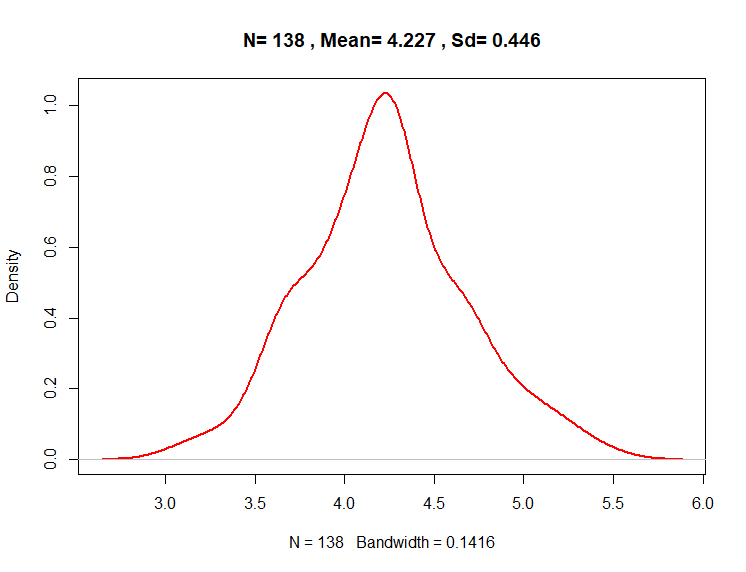
\includegraphics[width=0.49\linewidth,height=0.49\textheight]{image/Densitytest} 

}

\caption{正态分布检验与密度图}\label{fig:densitytest}
\end{figure}

\hypertarget{qq-plot}{%
\subsubsection{QQ-plot}\label{qq-plot}}

有的数据从直方图和密度图很难检验正态性,因此建议用qq图来确证这些图。QQ-plot,又称正态图。在QQ-plots中,
我们只需要确定数据点是否沿着直线(有时也称为Henry's line),而不是查看数据的扩散情况(如直方图和密度图)。
如果点靠近参考线并且在置信区间内,则认为满足了正态性假设。点与参考线之间的偏差越大,偏离置信区间越远,
满足正态条件的可能性就越小。这12个成年人的身高似乎服从正态分布,因为所有的点都在置信区间内。

如果qq图所示的非正态分布(系统地偏离参考线)时,通常第一步是对数据进行对数变换,
并重新检查对数变换后的数据是否正态分布。可以应用log()函数进行对数变换。

另外,qq图也是评估回归分析的残差是否服从正态分布的一种方便的方法。

\begin{figure}

{\centering 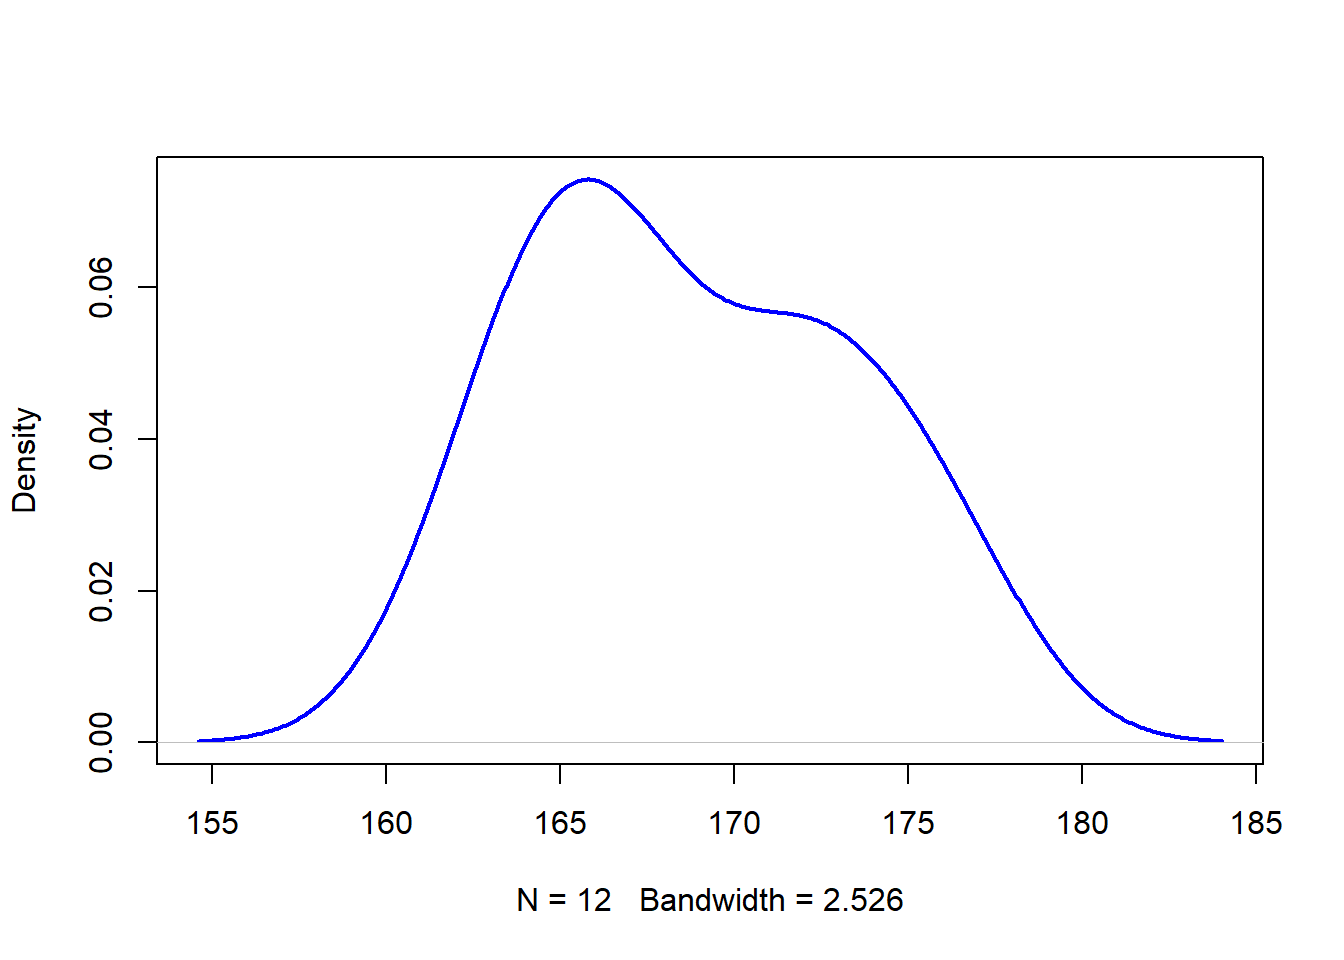
\includegraphics[width=0.49\linewidth,height=0.49\textheight]{figs/qqPlottest1} 

}

\caption{难以判断正态分布的密度图}\label{fig:qqPlottest1}
\end{figure}

\begin{Shaded}
\begin{Highlighting}[]
\CommentTok{#qqPlot是car包中的函数,因此需要载入包,可以使用groups参数,同时对多组数据分别处理}
\KeywordTok{library}\NormalTok{(car)}
\KeywordTok{set.seed}\NormalTok{(}\DecValTok{42}\NormalTok{)}
\NormalTok{dat_hist <-}\StringTok{ }\KeywordTok{data.frame}\NormalTok{( }\DataTypeTok{value =} \KeywordTok{rnorm}\NormalTok{(}\DecValTok{12}\NormalTok{, }\DataTypeTok{mean =} \DecValTok{165}\NormalTok{, }\DataTypeTok{sd =} \DecValTok{5}\NormalTok{))}
\KeywordTok{qqPlot}\NormalTok{(dat_hist}\OperatorTok{$}\NormalTok{value)}
\end{Highlighting}
\end{Shaded}

\begin{figure}

{\centering 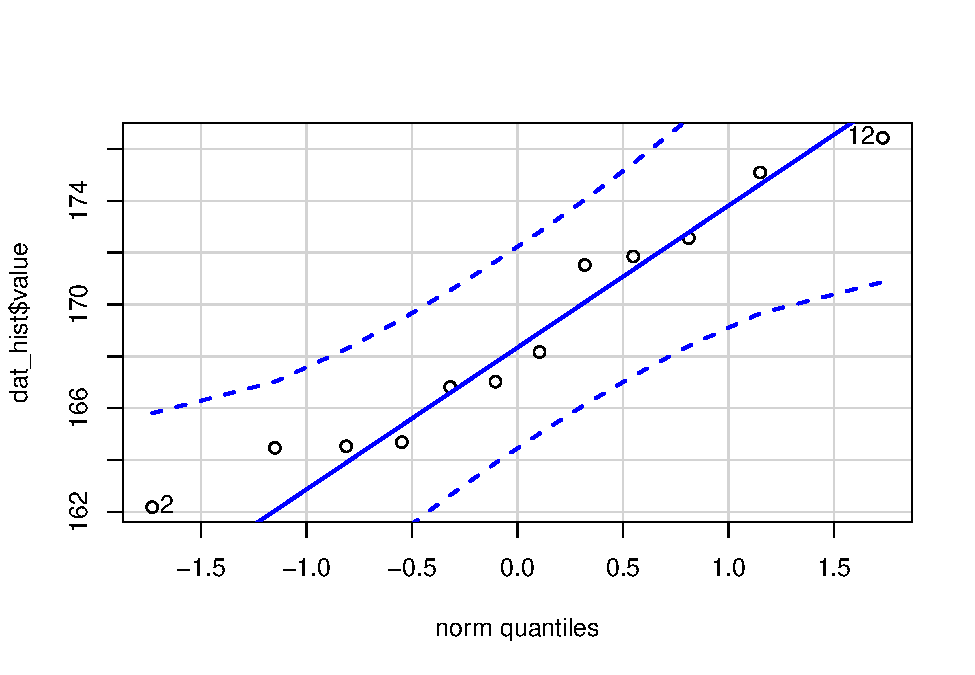
\includegraphics[width=0.49\linewidth,height=0.49\textheight]{figs/qqplot} 

}

\caption{正态分布检验与QQ-plot (1)}\label{fig:qqplot}
\end{figure}

\begin{Shaded}
\begin{Highlighting}[]
\KeywordTok{library}\NormalTok{(car)}
\KeywordTok{qqPlot}\NormalTok{(}\KeywordTok{as.numeric}\NormalTok{(RBC_v),}\DataTypeTok{ylab=}\StringTok{"RBC"}\NormalTok{, }\DataTypeTok{main=}\StringTok{"RBC QQ-plot"}\NormalTok{)}
\end{Highlighting}
\end{Shaded}

\begin{figure}

{\centering 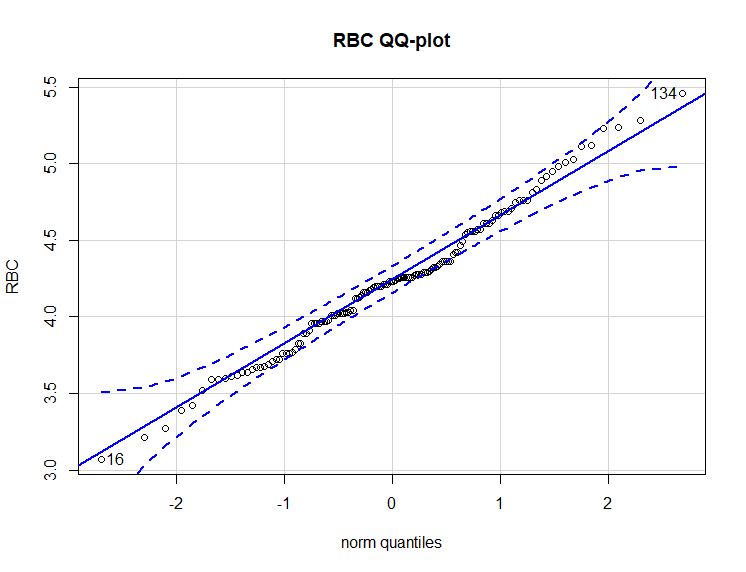
\includegraphics[width=0.49\linewidth,height=0.49\textheight]{image/qqPlot} 

}

\caption{正态分布检验与QQ-plot (2)}\label{fig:qqplot1}
\end{figure}

\hypertarget{ux6b63ux6001ux68c0ux9a8c}{%
\subsubsection{正态检验}\label{ux6b63ux6001ux68c0ux9a8c}}

上述3种方法是对常态的目视检查。然而,目测有时可能不可靠,因此也有可能通过统计检验正式检验数据是否服从正态分布。
这些正态性检验将数据的分布与正态分布进行比较,以评估观察结果是否显示出偏离正态性的重要偏差。
最常用的两种正态性检验是Shapiro-Wilk检验(K检验)和Kolmogorov-Smirnov检验(D检验)。两种测试都有相同的假设,即:

\textbf{\emph{H0}} : 数据服从正态分布

\textbf{\emph{H1}} : 数据不服从正态分布

正态性检验推荐使用Shapiro-Wilk检验,因为它比Kolmogorov-Smirnov检验提供更好的效用。
在R中,正态性的Shapiro-Wilk检验可以通过函数shapiro.test()进行。

\begin{Shaded}
\begin{Highlighting}[]
\KeywordTok{set.seed}\NormalTok{(}\DecValTok{42}\NormalTok{)}
\NormalTok{dat_hist <-}\StringTok{ }\KeywordTok{data.frame}\NormalTok{( }\DataTypeTok{value =} \KeywordTok{rnorm}\NormalTok{(}\DecValTok{12}\NormalTok{, }\DataTypeTok{mean =} \DecValTok{165}\NormalTok{, }\DataTypeTok{sd =} \DecValTok{5}\NormalTok{))}
\KeywordTok{shapiro.test}\NormalTok{(dat_hist}\OperatorTok{$}\NormalTok{value)}
\CommentTok{##      Shapiro-Wilk normality test}
\CommentTok{##  }
\CommentTok{##  data:  dat_hist$value}
\CommentTok{##  W = 0.9, p-value = 0.5}
\end{Highlighting}
\end{Shaded}

从输出中,我们看到p-value\textgreater0.05意味着我们不拒绝数据服从正态分布的原假设。
该检验与qq图的方向相同,qq图与正态性没有显著偏差(因为所有点都在置信区间内)。

\begin{Shaded}
\begin{Highlighting}[]
\KeywordTok{shapiro.test}\NormalTok{(RBC_v)}
\CommentTok{##      Shapiro-Wilk normality test}
\CommentTok{##  }
\CommentTok{##  data:  as.numeric(RBC_v)}
\CommentTok{##  W = 1, p-value = 0.4}
\end{Highlighting}
\end{Shaded}

对RBC数据同样的结果。

注意的是,在实践中,正态检验通常被认为过于保守,因为对于大样本(n\textgreater50),对正态条件的一个
小偏差可能会导致违反正态判断的条件。由于正态性检验是一种假设检验,所以随着样本量的增加,其检测较小差
异的能力也会增加。因此,随着观测数的增加,Shapiro-Wilk检验变得非常敏感,甚至对正态性的一个
微小偏差也非常敏感。所以,根据正态性检验,数据不服从正态分布,尽管偏离正态分布的情况可以忽略不计,但数据
实际上服从正态分布。因此,通常情况下,正态性条件的验证是基于本文所介绍的所有方法的组合,即目视检验
(使用直方图和q-q图)和正式化检验(例如使用shapio-wilk检验)。

R中还有其他一些正态检验的方法,比如 ks.test() 函数实现Kolmogorov-Smirnov Test(D检验),
是对经验分布的拟合检验,检验的是经验分布函数和假设总体分布函数的差异,适应于大样本(n\textgreater5000)。
另外有一些package包含了丰富的检验函数,比如fBasics,nortest等。

\hypertarget{ux7b2cux4e09ux7ae0-ux603bux4f53ux5747ux6570ux7684ux4f30ux8ba1ux4e0eux5047ux8bbeux68c0ux9a8c}{%
\section{第三章 总体均数的估计与假设检验}\label{ux7b2cux4e09ux7ae0-ux603bux4f53ux5747ux6570ux7684ux4f30ux8ba1ux4e0eux5047ux8bbeux68c0ux9a8c}}

日期: 2020-11-14
作者:wxhyihuan

\hypertarget{ux63a8ux8bbaux7edfux8ba1}{%
\subsection{推论统计}\label{ux63a8ux8bbaux7edfux8ba1}}

推论统计(或称统计推断,Statistical inference),指统计学中,研究如何根据样本数据去推断总体数量特征的方法。
它是在对样本数据进行描述的基础上,对统计总体的未知数量特征做出以概率形式表述的推断。更概括地说,
是在一段有限的时间内,通过对一个随机过程的观察来进行推断的。统计学中,统计推断与描述统计相对应。

推论统计(Statistical inferences)是借助抽样调查,从局部推断总体,以对不肯定的事物做出决策的一种统计。
有总体\emph{参数估计}与\emph{假设检验}两种。前者以一次性抽样实验为依据,对整个总体的某个数字特征做出估计。后者则是对
某种假设进行检验,根据计算结果推断所做的假设是否可以接受。如平均数、标准差、相关系数、回归系数等特征的
总体估计及差异显著性检验。推断统计的理论基础是概率论,它更多地需要借助抽样理论与方法。

\hypertarget{ux53c2ux6570ux4f30ux8ba1ux4e0eux5047ux8bbeux68c0ux9a8c}{%
\subsubsection{参数估计与假设检验}\label{ux53c2ux6570ux4f30ux8ba1ux4e0eux5047ux8bbeux68c0ux9a8c}}

参数估计背后的思想是通过对从总体中抽取的样本进行统计显著性检验(如t检验),为研究人员提供关于总体的统计推断。
最常用的就是t检验,其参数检验是基于W.S.Gosset的t统计量,该统计数据假设变量来自正态总体。t检验统计量中的总体均值是已知的。
这种分布称为t分布,其形状与正态分布类似,即钟形曲线。t检验用于检验那些样本小于30的样本比正态分布要好,
在大样本上做的和正态分布一样好。

假设检验(Hypothesis test)过去也叫做显著性检验(Significance test),是利用小概率反证法思想,从问题的对立面(\(H_0\))出发,
间接判断解决问题(\(H_1\))是否成立。即在假设\(H_0\)成立的条件下,计算检验统计量(Test static),然后根据\(P\)值(P-value)来判断。

\hypertarget{ux7edfux8ba1ux91cfux4e0eux6807ux51c6ux8bef}{%
\subsubsection{统计量与标准误}\label{ux7edfux8ba1ux91cfux4e0eux6807ux51c6ux8bef}}

样本是总体的代表和反映,也是统计推断的依据,为了对总体的分布或数字特征进行各种统计推断,还需要对样本作加工处理,
把样本中应关心的事物和信息集中起来,针对不同的问题构造出样本的不同函数(如均值,方差,极差,标准差,中位数,众数等),这种样本的函数我们称其为统计量。

样本统计量的标准差即为标准误(Stand error,SE),反映了抽样的统计量的离散程度或误差大小。如样本均数的标准差也称为均数标准误
(Stand error of mean, SEM),反映了样本均数的离散程度。

\hypertarget{t-ux5206ux5e03}{%
\subsection{\texorpdfstring{\emph{t} 分布}{t 分布}}\label{t-ux5206ux5e03}}

若某一随机变量\emph{X}服从总体均数为\emph{μ},总体标标准差为\emph{σ}的正态分布\(N(μ,σ^2)\),通过\emph{u}变换(也称Z变换)可将一般正态分布
转化为标准正态分布\(N(0,1^2)\),即u分布(也称Z分布)。同理,若样本含量为n的样本均数 \(\bar{X}\) 服从总体均数为\emph{μ},
总体标准差为\(σ_\bar{x}\)的正态分布\(N(μ,σ_\bar{x}^2)\),则可通过\emph{u}变换(\(\frac{\bar{X}-μ}{σ_\bar{x}}\))将其转换为标准正态分布。
但是,实际中总体标准差(\(σ_\bar{x}\))是未知的,所以用均数标准误的估计值(\(S_\bar{x}=\frac{S}{\sqrt{n}}\),其中S为样本标准差)代替,
这就使得(\(\frac{\bar{X}-μ}{S_\bar{x}}\))不再是标准正态分布,而是服从t-分布(t-distribution),
即:
\[t=\frac{\bar{X}-μ}{S_\bar{x}}=\frac{\bar{X}-μ}{\frac{S}{\sqrt{n}}}\]

t-分布 对应的概率密度函数是:
\[f(x)=\frac{\Gamma(\frac{v+1}{2})}{\sqrt{v\pi}\Gamma(\frac{v}{2})}{\left(1+\frac{x^2}{v}\right)^\frac{-v+1}{2}}\]

其中\(\Gamma\)是伽马函数(Gamma function),\(v\)是自由度(Degree of freedom,df)。

\textbf{自由度(df)}在数学上只能自由取值的变量个数,如\(X+Y+Z=1\),有3个变量,但是能够自由取值的自由两个,故其自由度\(v=2\)。
在统计学中,自由度计算方式为:
\[v=n-m\]

其中\emph{n}为计算某一统计量是用到的数据个数,\emph{m}为计算该统计量是用到的其他独立统计量个数。比如根据肿瘤位置,大小,组织活检,生化指标
判断肿瘤的类型是A,也可能是B,这里有\(n=4\)个独立的信息,和\(m=2\)个估计,所以自由度就是\(df=4-2=2\)。一般的希望估计(推测)的越可靠,
当然是自由度越大越好了。

t分布是一簇曲线,其形态变化与n(即其自由度)大小有关。自由度n越小,t分布曲线越低平;自由度n越大,t分布曲线越接近标准正态分布(u分布)
曲线,当自由度无限大时,t分布就成了正态分布。

\hypertarget{ux6982ux7387ux5bc6ux5ea6ux51fdux6570dt}{%
\subsubsection{概率密度函数dt()}\label{ux6982ux7387ux5bc6ux5ea6ux51fdux6570dt}}

R中,t分布的概率密度函数为dt(),它可以给出了指定均值和标准差下每个点的概率分布的高度,
越高就代表着这个点/区间的概率越密集(大)。从下免得概率密度图见,当df=20时,t分布曲线已经非常接近标准正态曲线了。

\begin{Shaded}
\begin{Highlighting}[]
\KeywordTok{curve}\NormalTok{(}\KeywordTok{dnorm}\NormalTok{(x),}\DataTypeTok{xlim=}\KeywordTok{c}\NormalTok{(}\OperatorTok{-}\DecValTok{5}\NormalTok{,}\DecValTok{5}\NormalTok{),}\DataTypeTok{ylim=}\KeywordTok{c}\NormalTok{(}\DecValTok{0}\NormalTok{,}\FloatTok{0.45}\NormalTok{),}\DataTypeTok{ylab=}\StringTok{"Student's t Density"}\NormalTok{,}\DataTypeTok{col=}\StringTok{"red"}\NormalTok{,}\DataTypeTok{lty=}\DecValTok{1}\NormalTok{,}\DataTypeTok{lwd=}\DecValTok{2}\NormalTok{)}
\KeywordTok{abline}\NormalTok{(}\DataTypeTok{v=}\DecValTok{0}\NormalTok{,}\DataTypeTok{lwd=}\DecValTok{1}\NormalTok{,}\DataTypeTok{col=}\StringTok{"black"}\NormalTok{)}
\KeywordTok{curve}\NormalTok{(}\KeywordTok{dt}\NormalTok{(x,}\DecValTok{1}\NormalTok{),}\DataTypeTok{col=}\StringTok{"green"}\NormalTok{,}\DataTypeTok{lty=}\DecValTok{2}\NormalTok{,}\DataTypeTok{add=}\OtherTok{TRUE}\NormalTok{)}
\KeywordTok{curve}\NormalTok{(}\KeywordTok{dt}\NormalTok{(x,}\DecValTok{2}\NormalTok{),}\DataTypeTok{col=}\StringTok{"brown"}\NormalTok{,}\DataTypeTok{lty=}\DecValTok{3}\NormalTok{,}\DataTypeTok{add=}\OtherTok{TRUE}\NormalTok{)}
\KeywordTok{curve}\NormalTok{(}\KeywordTok{dt}\NormalTok{(x,}\DecValTok{5}\NormalTok{),}\DataTypeTok{col=}\StringTok{"blue"}\NormalTok{,}\DataTypeTok{lty=}\DecValTok{4}\NormalTok{,}\DataTypeTok{add=}\OtherTok{TRUE}\NormalTok{)}
\KeywordTok{curve}\NormalTok{(}\KeywordTok{dt}\NormalTok{(x,}\DecValTok{20}\NormalTok{),}\DataTypeTok{col=}\StringTok{"dark green"}\NormalTok{,}\DataTypeTok{lty=}\DecValTok{5}\NormalTok{,}\DataTypeTok{add=}\OtherTok{TRUE}\NormalTok{)}
\KeywordTok{legend}\NormalTok{(}\DecValTok{2}\NormalTok{,}\FloatTok{0.38}\NormalTok{,}\KeywordTok{c}\NormalTok{(}\StringTok{"normal"}\NormalTok{,}\StringTok{"df=1"}\NormalTok{,}\StringTok{"df=2"}\NormalTok{,}\StringTok{"df=5"}\NormalTok{,}\StringTok{"df=20"}\NormalTok{),}
       \DataTypeTok{col=}\KeywordTok{c}\NormalTok{(}\StringTok{"red"}\NormalTok{,}\StringTok{"green"}\NormalTok{,}\StringTok{"brown"}\NormalTok{,}\StringTok{"blue"}\NormalTok{,}\StringTok{"dark green"}\NormalTok{),}\DataTypeTok{lty=}\DecValTok{1}\OperatorTok{:}\DecValTok{5}\NormalTok{)}
\end{Highlighting}
\end{Shaded}

\begin{figure}

{\centering 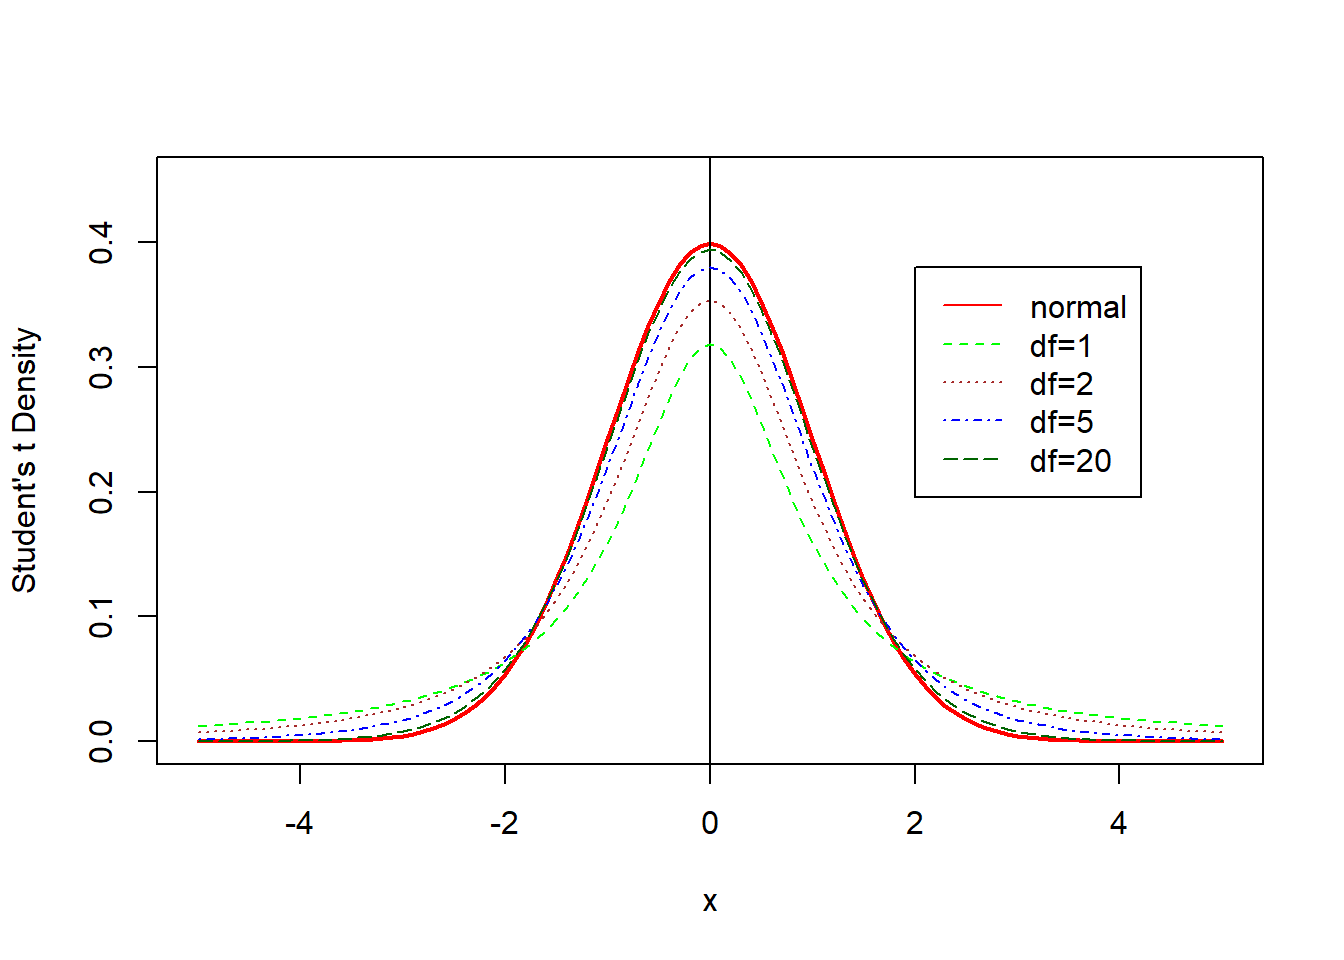
\includegraphics[width=0.49\linewidth,height=0.49\textheight]{figs/tdist} 

}

\caption{t分布检验与正态分布}\label{fig:tdist}
\end{figure}

\hypertarget{ux6982ux7387ux7d2fux79efux5206ux5e03ux51fdux6570pt}{%
\subsubsection{概率累积分布函数pt()}\label{ux6982ux7387ux7d2fux79efux5206ux5e03ux51fdux6570pt}}

同所有连续数值型分布一样,统计应用中最关心的是分布曲线下的尾部面积(即概率\(P\)或α)与横轴间的关系。
R中即为pt(),它给出一个正态分布中小于一个给定数字的累计概率(即指定定点的左边范围的曲线面积)。
一侧尾部面积称为单侧概率或单尾概率(one-tailed probability,\(t_{α,v}\)),两侧尾部的面积之和称为双侧概率或双尾概率
(two-tailes probability,\(t_{α/2,v}\))。

\textbf{单侧的p值计算}

\begin{Shaded}
\begin{Highlighting}[]
\CommentTok{# t-stat=1.9, df=5}
\CommentTok{# 单侧 p值}
\CommentTok{# P(t => 1.9)}
\KeywordTok{pt}\NormalTok{(}\DataTypeTok{q=}\FloatTok{1.9}\NormalTok{, }\DataTypeTok{df=}\DecValTok{5}\NormalTok{, }\DataTypeTok{lower.tail =}\NormalTok{ F)}
\CommentTok{## [1] 0.05793165}
\end{Highlighting}
\end{Shaded}

\textbf{双侧的p值计算}

\begin{Shaded}
\begin{Highlighting}[]
\CommentTok{## 双侧 p-value}
\CommentTok{## 两边对称单侧相加}
\KeywordTok{pt}\NormalTok{(}\DataTypeTok{q=}\FloatTok{1.9}\NormalTok{, }\DataTypeTok{df=}\DecValTok{5}\NormalTok{, }\DataTypeTok{lower.tail =}\NormalTok{ F) }\OperatorTok{+}\StringTok{ }\KeywordTok{pt}\NormalTok{(}\DataTypeTok{q=}\OperatorTok{-}\FloatTok{1.9}\NormalTok{, }\DataTypeTok{df=}\DecValTok{5}\NormalTok{, }\DataTypeTok{lower.tail =}\NormalTok{ T)}
\CommentTok{## 0.1158633}
\CommentTok{## 单侧p值*2,对称性}
\KeywordTok{pt}\NormalTok{(}\DataTypeTok{q=}\FloatTok{1.9}\NormalTok{, }\DataTypeTok{df=}\DecValTok{5}\NormalTok{, }\DataTypeTok{lower.tail =}\NormalTok{ F)}\OperatorTok{*}\DecValTok{2}
\CommentTok{## 0.1158633}
\end{Highlighting}
\end{Shaded}

\begin{Shaded}
\begin{Highlighting}[]
\CommentTok{# x坐标序列向量}
\NormalTok{x_pt <-}\StringTok{ }\KeywordTok{seq}\NormalTok{(}\OperatorTok{-}\StringTok{ }\DecValTok{5}\NormalTok{, }\DecValTok{5}\NormalTok{, }\DataTypeTok{by =} \FloatTok{0.1}\NormalTok{)}
\CommentTok{# 用pt()函数获取df=5的x累计密度值}
\NormalTok{y_pt <-}\StringTok{ }\KeywordTok{pt}\NormalTok{(x_pt, }\DataTypeTok{df =} \DecValTok{5}\NormalTok{)}
\CommentTok{# Plotting }
\KeywordTok{plot}\NormalTok{(y_pt, }\DataTypeTok{type =} \StringTok{"l"}\NormalTok{, }\DataTypeTok{main =} \StringTok{"t-distribution cumulative function example"}\NormalTok{, }\DataTypeTok{las=}\DecValTok{1}\NormalTok{, }\DataTypeTok{col=}\StringTok{"red"}\NormalTok{,}\DataTypeTok{lwd=}\DecValTok{2}\NormalTok{)}
\end{Highlighting}
\end{Shaded}

\begin{figure}

{\centering 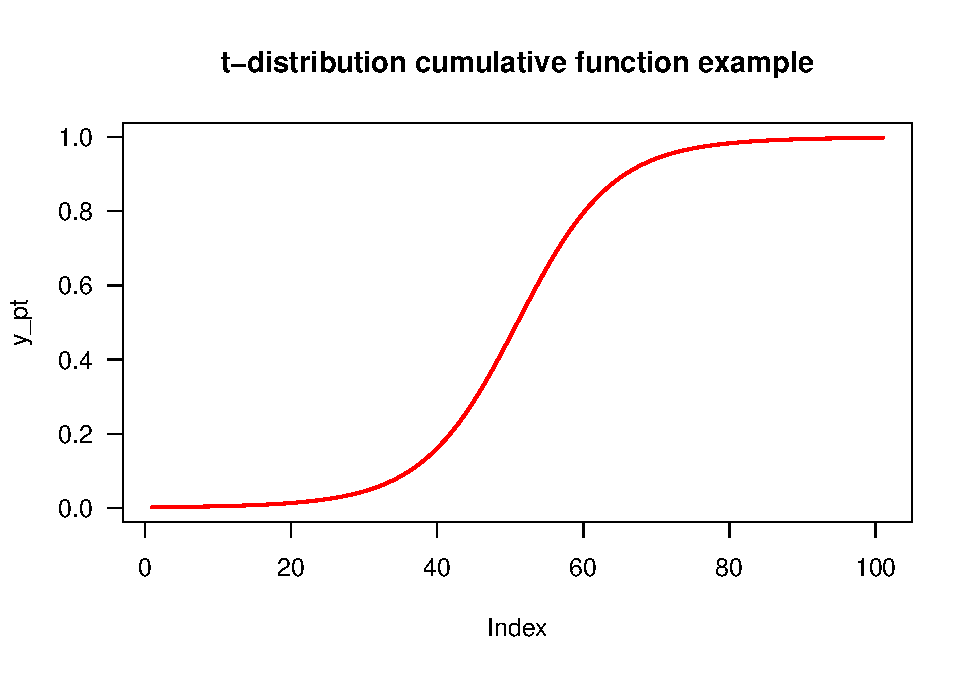
\includegraphics[width=0.49\linewidth,height=0.49\textheight]{figs/pttest} 

}

\caption{t分布的pt()}\label{fig:pttest}
\end{figure}

\hypertarget{ux6c42ux7f6eux4fe1ux533aux95f4ux7684qt}{%
\subsubsection{求置信区间的qt()}\label{ux6c42ux7f6eux4fe1ux533aux95f4ux7684qt}}

t分布分位函数,R中即为qt(),它可以给出一个累积分布概率达到指定值的数字。

\begin{Shaded}
\begin{Highlighting}[]
\CommentTok{# find t for 95% confidence interval value of t with 2.5% in each tail}
\KeywordTok{qt}\NormalTok{(}\DataTypeTok{p=}\FloatTok{0.025}\NormalTok{, }\DataTypeTok{df =} \DecValTok{5}\NormalTok{, }\DataTypeTok{lower.tail =}\NormalTok{ T)}
\CommentTok{## -2.570582}
\end{Highlighting}
\end{Shaded}

\begin{Shaded}
\begin{Highlighting}[]
\CommentTok{# Specifyin the x-values}
\NormalTok{x_qt <-}\StringTok{ }\KeywordTok{seq}\NormalTok{(}\FloatTok{0.1}\NormalTok{, }\DataTypeTok{by =} \FloatTok{0.01}\NormalTok{)}
\CommentTok{# Applying the qt() function}
\NormalTok{y_qt <-}\StringTok{ }\KeywordTok{qt}\NormalTok{(x_qt, }\DataTypeTok{df =} \DecValTok{5}\NormalTok{)}
\CommentTok{# Plotting}
\KeywordTok{plot}\NormalTok{(y_qt, }\DataTypeTok{main =} \StringTok{"t quantile function example"}\NormalTok{, }\DataTypeTok{las =} \DecValTok{1}\NormalTok{,}\DataTypeTok{col=}\StringTok{"red"}\NormalTok{,}\DataTypeTok{lwd=}\DecValTok{2}\NormalTok{)}
\end{Highlighting}
\end{Shaded}

\begin{figure}

{\centering 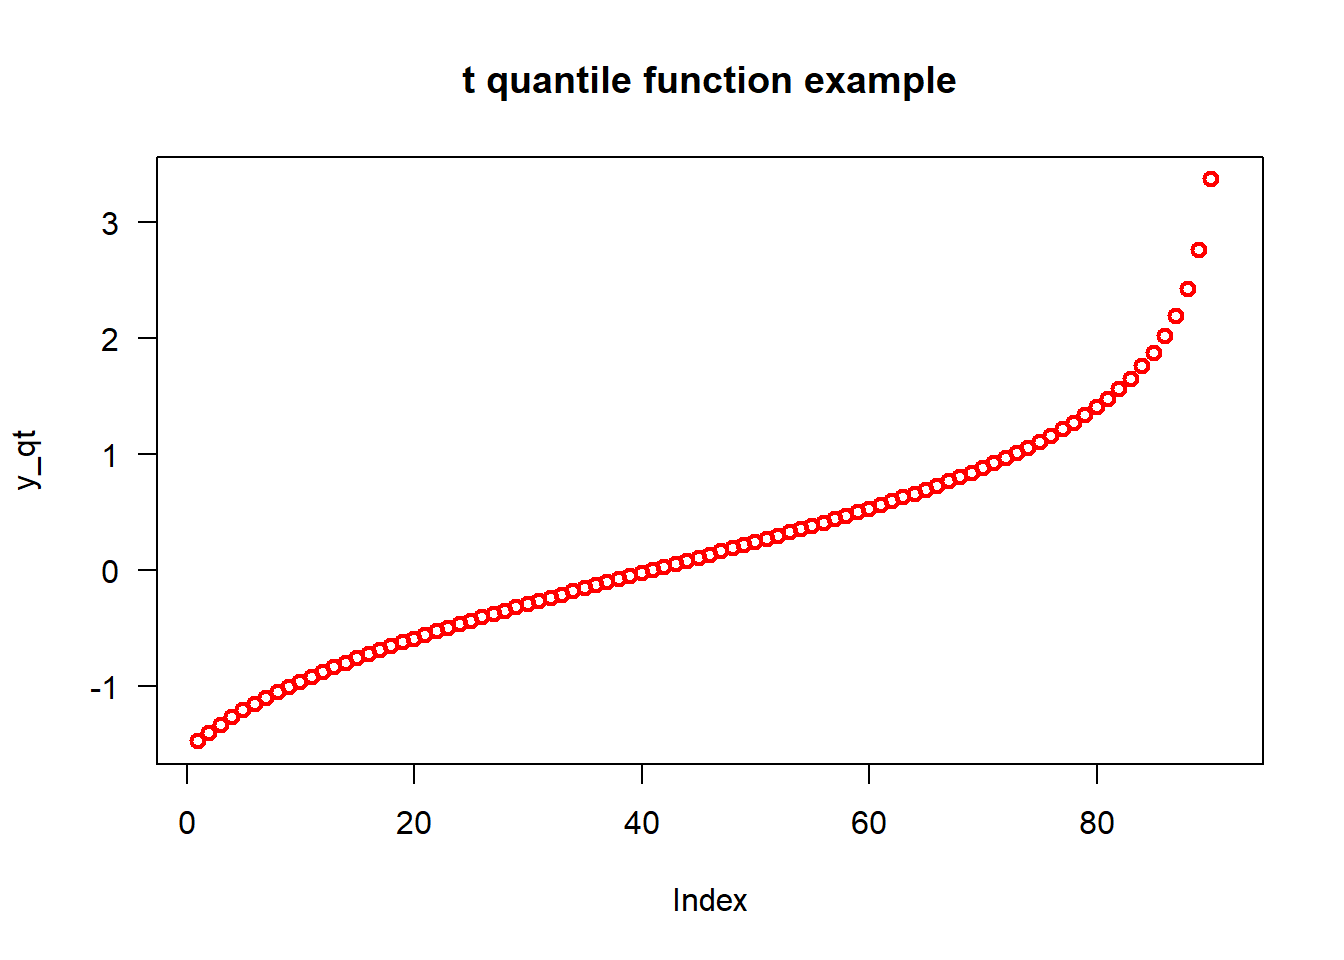
\includegraphics[width=0.49\linewidth,height=0.49\textheight]{figs/qttest} 

}

\caption{t分布的qt()}\label{fig:qttest}
\end{figure}

\hypertarget{ux6307ux5b9atux5206ux5e03ux51fdux6570rt}{%
\subsubsection{指定t分布函数rt()}\label{ux6307ux5b9atux5206ux5e03ux51fdux6570rt}}

rt()函数用于生成符合指定观测数目和自由度的t分布的随机数,默认是。

\begin{Shaded}
\begin{Highlighting}[]
\KeywordTok{set.seed}\NormalTok{(}\DecValTok{61}\NormalTok{)}
\CommentTok{# Setting sample size}
\NormalTok{n <-}\StringTok{ }\DecValTok{10000}
\CommentTok{# Using rt() to drawing N log normally distributed values}
\NormalTok{y_rt <-}\StringTok{ }\KeywordTok{rt}\NormalTok{(n, }\DataTypeTok{df =} \DecValTok{5}\NormalTok{)}
\CommentTok{# Plotting a histogram of y_rt}
\KeywordTok{hist}\NormalTok{(y_rt, }\DataTypeTok{breaks =} \DecValTok{100}\NormalTok{, }\DataTypeTok{main =} \StringTok{"Randomly drawn t density"}\NormalTok{, }\DataTypeTok{freq=}\OtherTok{FALSE}\NormalTok{,}
  \DataTypeTok{col=}\StringTok{"#A8D6FF"}\NormalTok{,}\DataTypeTok{xlim=}\KeywordTok{c}\NormalTok{(}\OperatorTok{-}\DecValTok{10}\NormalTok{,}\DecValTok{10}\NormalTok{),}\DataTypeTok{ylim=}\KeywordTok{c}\NormalTok{(}\DecValTok{0}\NormalTok{,}\FloatTok{0.4}\NormalTok{))}
\KeywordTok{lines}\NormalTok{(}\KeywordTok{density}\NormalTok{(y_rt), }\DataTypeTok{col=}\StringTok{"red"}\NormalTok{, }\DataTypeTok{lwd=}\DecValTok{2}\NormalTok{)}
\end{Highlighting}
\end{Shaded}

\begin{figure}

{\centering 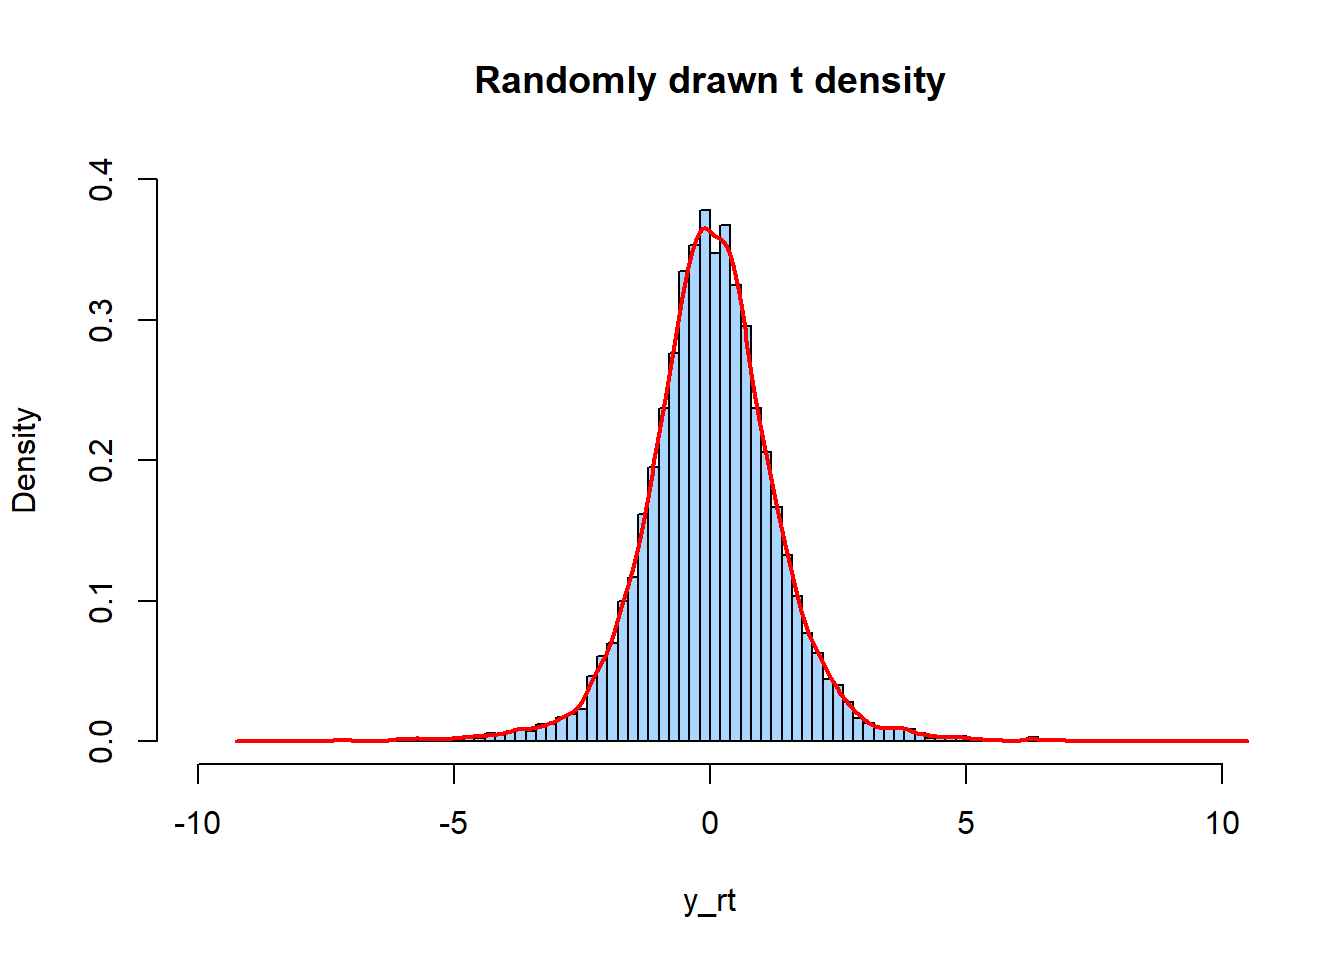
\includegraphics[width=0.49\linewidth,height=0.49\textheight]{figs/rttest} 

}

\caption{t分布的rt()}\label{fig:rttest}
\end{figure}

\hypertarget{ux53c2ux6570ux4f30ux8ba1}{%
\subsubsection{参数估计}\label{ux53c2ux6570ux4f30ux8ba1}}

参数估计是指用样本参数(统计量)推断总体参数,有点值估计(Point estimation)和区间估计(Interval estimation)两种。

\textbf{点值估计}就是用相应样本统计量简单直接的作为总体参数的估计值,如用\(\bar{X}\)估计\(μ\),用\(S\)估计\(\sigma\)。
案例 某开发团队对开发App进行了改版迭代,现在有以下两个版本
+ 版本1: 首页为一屏课程列表
+ 版本2:首页为信息流
如果我们想区分两个版本,哪个版本用户更喜欢,转化率会更高。我们就需要对总体(全部用户)进行评估,
但是并不是全部存量用户都会访问App,并且每天还会新增很多用户,所以我们无法对总体(全部用户)进行评估,
我们只能从总体的用户中随机抽取样本(访问App)的用户进行分析,用样本数据表现情况来充当总体数据表现情况,
以此来评估哪个版本转化率更高。

\textbf{区间估计}是按预先给定概率(\(1-\alpha\)),通过特定的分布函数来计算确定的未知总体参数的范围。该范围称为参数的可信区间或

置信区间(Confidence bound/Confidence interval,\emph{CI}),预先设定的概率\((1-\alpha)\)称为可信度或置信度(Confidence level),
通常取值95\%或99\%,如果特殊说明,一般是双侧95\%。可信区间是两个字确定的范围,其中较小的值称为可信下限(Lower limit,L),
较大值称为可行上限(Upper limit,U),表示为开区间(L,U)。

\hypertarget{ux603bux4f53ux5747ux6570ux53efux4fe1ux533aux95f4}{%
\paragraph{总体均数可信区间}\label{ux603bux4f53ux5747ux6570ux53efux4fe1ux533aux95f4}}

\href{https://zh.wikipedia.org/wiki/\%E7\%BD\%AE\%E4\%BF\%A1\%E5\%8C\%BA\%E9\%97\%B4}{可信区间的计算}是从已知总体中进行固定样品含量的重复随机抽样实验,根据每个样本计算的可信区间。可信区间的好坏取决于①可信度\(1-\alpha\)
的大小;②是区间的宽度,通过增加样本含量可以缩减区间宽度。

1.单一总体均数可信区间

\begin{itemize}
\item
  a.\(\sigma\)未知且\(n\)较小(n≤60)时,按照t分布计算。
\item
  b.\(\sigma\)未知且\(n\)较大(n>60)时,按照标准正态分布(即u分布或Z分布)计算。
\end{itemize}

计算公式和示例可参见教材或者\href{https://zh.wikipedia.org/wiki/\%E7\%BD\%AE\%E4\%BF\%A1\%E5\%8C\%BA\%E9\%97\%B4}{百科资料}。

2.两总体均数之差的可信区间

\begin{itemize}
\tightlist
\item
  参见教材或者\href{https://zh.wikipedia.org/wiki/\%E7\%BD\%AE\%E4\%BF\%A1\%E5\%8C\%BA\%E9\%97\%B4}{百科资料}。
\end{itemize}

\hypertarget{ux5047ux8bbeux68c0ux9a8c}{%
\subsubsection{假设检验}\label{ux5047ux8bbeux68c0ux9a8c}}

从总体中随机抽样,由样本信息推断总体特征,除前面所讲的参数估计方法外,在实际应用中还会遇到这样的问题:某一样本均数是
否来自于某已知数的总体?两个不同样本均数是否来自均数不相等的总体等要回答这类问题,除可用前面参数估计的方法外,
更多的是用统计推断的另一方面------假设检验 (Hypothesis test)来解决,比如下面两个案例:

\textbf{案例3-5} 某医生测量了36名从事铅作业男性工人的血红蛋白含量,算得其均数为130.83 g/L,标准差为25.74 g/L。问:
从事铅作业男性工人的血红蛋白含量均数(\emph{μ})是否不等于正常成年男性的均数 140 g/L (\(μ_0\))?

针对问题一,其目的是判断是否\(μ≠μ_0\),以给出的条件看\(\bar{X}\)与已知总体均数\(μ_0\)不相等,
造成两者不等的原因有两种情况:

①从事前作业的样品血红含量确实与正常样品不一样,即非同一总体(\(μ≠μ_0\));

②因为抽样误差导致的两者不相等,两者实际为同一总体(\(μ=μ_0\))。

要判断第一种情况很困难,但可以利用反正思想从第②种出发,间接判断是否\(μ≠μ_0\):假设\(μ=μ_0\),判断由于抽样误
差造成不相等的可能行有多大?

如果\(\bar{X}\)与\(μ_0\)接近,其差别可用抽样误差解释,即可认为\(\bar{X}\)来自\(μ_0\)总体。反之,相差很大,
则难以说明\(\bar{X}\)来自\(μ_0\)总体。那么,\(\bar{X}\)与\(μ_0\)相差多大算是抽样误差造成的呢?若假设(\(μ=μ_0\))成立,
且样本总体符合正态分布(本案例未进行进一步判断,针对实际数据情况,做假设检验前应该情况进行分布判断或转换处理,选择合适的检验方法),
则可以用t分布(\(t=\frac{\bar{X}-μ}{S/\sqrt{n}}\))或正态分布(\(u=\frac{\bar{X}-μ}{\sigma/\sqrt{n}}\))
来计算t值或者u值。然后根据t值或u值求得P值(P-value)来判断。如果\(\bar{X}\)与\(μ_0\)相差很大,那么t或者u值就很大,
对应P值就小;当P值小于或等于预先规定的概率值α(如0.05)时,则为小概率事件,这有理由怀疑原假设(\(μ=μ_0\))可能不成立,
认为其对立面(\(μ≠μ_0\))成立,该结论的正确性冒着5\%的错误风险。

\hypertarget{ux5047ux8bbeux68c0ux9a8cux7684ux6b65ux9aa4}{%
\paragraph{假设检验的步骤}\label{ux5047ux8bbeux68c0ux9a8cux7684ux6b65ux9aa4}}

\textbf{1. 建立检验假设,确定检验水准}

\begin{itemize}
\item
  有两种假设,即\(H_0\)和\(H_1\):

  \begin{itemize}
  \item
    (1)\(μ=μ_0\),即检验假设(Hypothsis under test),称为无效假设,也叫做零假设,原假设(Null hypothsis),
    用\(H_0\)表示,原假设的设置一般为:等于=、大于等于\textgreater=、小于等于\textless=。
  \item
    (2)\(μ≠μ_0\),即备择假设(Alternative test),也称为对立假设,用\(H_1\)表示,备择假设的设置一般为:不等于、大于\textgreater、小于\textless。
  \end{itemize}
\end{itemize}

~ 对检验假设,需要注意以下几点

~ ①. 检验假设针对的是总体,而不是样本;

~ ②. \(H_0\)和\(H_1\)是相互联系,对你的假设,后面的统计推断的结论是根据\(H_0\)和\(H_1\)作出的,二者缺一不可;

~ ③. \(H_0\)为无效假设,其假定通常是:某两个(或多个)总体的参数相等,或两个总体参数之差为0,或某资料服从某一特定分布
~ (如正态分布,Poisson分布等),或\(\cdots\cdots\)无效等;

~ ④. \(H_1\)的内容直接反映呢检验的单双侧。比如案例3-5中,如果\(μ≠μ_0\),则此检验为双侧检验(Two-sided test);若\(H_1\)为
~ \(μ>μ_0\)或\(μ小于μ_0\),则检验为单侧检验(One-sided test),不仅考虑差异,而且考虑差异的方向。单双侧检验的确定,
~ 首先需要根据专业知识,其次是根据需要解决的问题来确定。

\begin{itemize}
\tightlist
\item
  检验水准α,也称显著性水准(Singnificance level),它属于Ⅰ型错误的范畴,是预先规定的概率值,它确定了
  小概率事件的标准。实际中常取\(\alpha=0.05\),可根据不同研究目的给予不同设置。
\end{itemize}

\begin{center}\rule{0.5\linewidth}{0.5pt}\end{center}

\textbf{第I类错误和第Ⅱ类错误}

为什么统计者想要拒绝的假设放在原假设呢?因为原假设备被拒绝如果出错的话,只能犯第I类错误,而犯第I类错误的概率已经
被规定的显著性水平所控制。

我们通过样本数据来判断总体参数的假设是否成立,但样本是随机抽取的,因而有可能出现小概率的错误。这种小概率错误有两种,
一种是第I类错误(也叫弃真错误,Type Ⅰ error),另一种是第Ⅱ类错误(也叫取伪错误,Type Ⅱ error)。

第I类错误或α错误:它是指\(H_0\)实际上是真的,但通过假设检验后,拒绝了原假设。这是错误的,
我们拒绝了真实的原假设,所以叫弃真错误,这个错误的概率我们记为α,也就是检验水准。在假设检验之前我们会规定这个概率的大小,从而控制检验功效。

第II类错误或β错误:它是指\(H_0\)实际上假的,但通过假设检验显示,不拒绝原假设。这也是错误的,我们接受的原假设实际上是假的,所以叫取伪错误,这个错误的概率我们记为β。

1-β称为检验效能(Power of test),过去称把握度。其意义为当两总体确有差异,按规定检验水准α所能发现该差异的能力。
和B一样,1-β只取单尾。如1-β = 0.90,意味着若两总体确有差别,则理论上平均每100 次检验中,有90 次能够得出差异
有统计学意义的结论。从图中可看出,α愈小,B愈大; 反之α愈大,β愈小。若要同时减小型错误a以及1型错误B,唯一的方法
就是增加样本含量n。若重点是减少第I类错误α(如一般的假设检验),一般取 a=0.05。
若重点是减少第II类错误(如方差齐性检验,正态性检验或想用一种方法代替另一种方法的检验等),
一般取 a = 0.10 或0.20,甚至更高。注意:拒绝\(H_0\),只可能犯第I类错误,不可能第II类错误。
不拒绝\(H_0\),只可能犯第II类错误,不可能犯第I类错误。

因此,原假设一般都是想要拒绝的假设,如果原假设备被错误拒绝的话,只能犯弃真错误,而犯弃真错误的概率可以用
检验水准\(\alpha\)控制,对统计者来说更容易控制,将错误影响降到最小。

\begin{figure}

{\centering 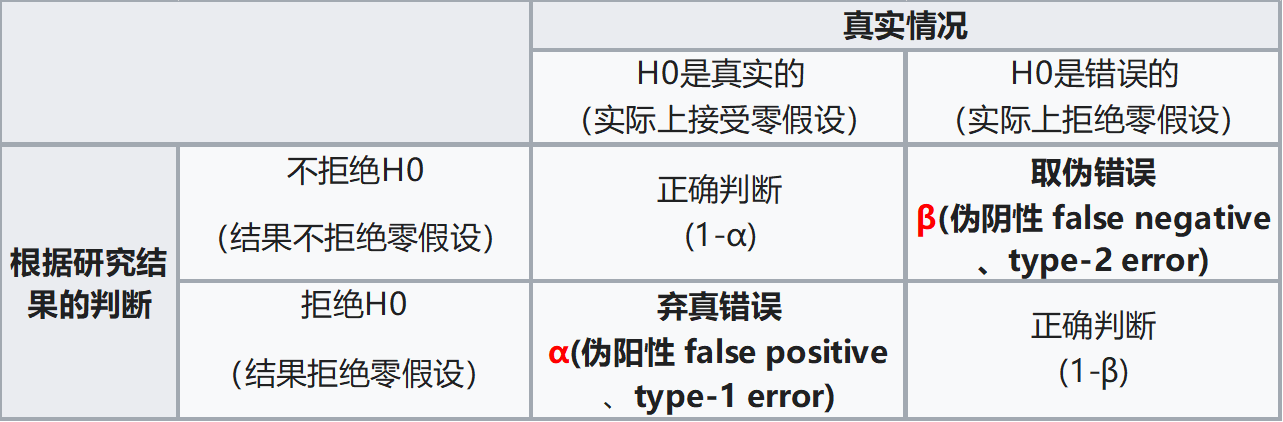
\includegraphics[width=0.49\linewidth,height=0.49\textheight]{image/type12error} 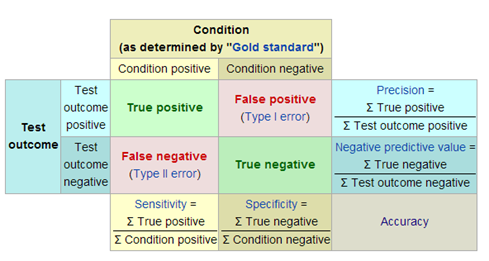
\includegraphics[width=0.49\linewidth,height=0.49\textheight]{image/type12error_en} 

}

\caption{第I类错误和第Ⅱ类错误}\label{fig:typeerror}
\end{figure}

\begin{center}\rule{0.5\linewidth}{0.5pt}\end{center}

\textbf{2. 计算检验统计量}

\begin{itemize}
\item
  应该根据变量或资料的类型,设计方案,统计推断的目的,方法的适用条件等选择检验统计量。如成组设计两样本均数的比较可根据
  资料特点选用检验统计量\(t,t',u\)等;而成组设计两样本翻查的比较一般先用检验统计量\(F\)。计算这些统计量都是在\(H_0\)(\(μ=μ_0\)),
  即假定是比较的数据来自同一总体的成立前提下算出来的。
\item
  有的检验方法无需计算检验统计量,如四个表资料。
\end{itemize}

\textbf{3. 确定\(P\)值,做出推断结论}

\(P\)的含义是指从\(H_0\)规定的总体中随机抽样,抽得等于及大于或(和)等于及小于现有样本获得的统计量(如\(t\)、\(u\)等)值的概率。
根据获得的时候概率\(P\)值,与之相规定的检验水准\(\alpha\)进行比较,看其是否为小概率事件二得出结论。
一般来说,推断结论应包含统计结论和专业结论两部分,前者只说明差异是否有统计学意义(Statistical Significance),
后者这是结合专业内容给出的结论解释:

\begin{itemize}
\item
  \(P\leq\alpha\),则发生小概率事件,拒绝\(H_0\),接受\(H_1\),差异具有统计学意义。
\item
  \(P>\alpha\),则不拒绝\(H_0\),差异无统计学意义。\(P>\alpha\)也成为``无显著性''(Non-Significance,NS),即阴性结果。
\end{itemize}

注意的是:

① 不拒绝\(H_0\)不等于接受\(H_0\),虽然在逻辑上否定的否定为肯定,但在统计上是按照检验水准\(\alpha\)不拒绝\(H_0\),若接受\(H_0\)
则因为范Ⅱ型错误的概率\(\beta\)未知而证据不足,以决策的观点,之客认为展示有条件``接受'',或``阴性待诊''。

② 作结论是,对\(H_0\)只能说拒绝(Reject)或者不拒绝(Not reject)\(H_0\)。而对\(H_1\)只能说接受\(H_1\),其他说法俱不妥当。

③ 差异有无统计学意义,是对样本统计量和总体参数(如\(\bar{X}\)和\(μ_0\)),或两个,多个样本统计量(如\(\bar{X_1}\)和\(\bar{X_2}\))而言,
对推断两个总体参数(如\(μ_1\)和\(μ_0\),或\(μ_1\)和\(μ_2\))而言,只能说是否相等。

\textbf{拒绝域}
拒绝域是由显著性水平围成的区域。拒绝域的功能主要用来判断假设检验是否拒绝原假设的。如果样本观测计算出来的
检验统计量(如\emph{t},\emph{u}值)的具体数值落在拒绝域内,就拒绝原假设,否则不拒绝原假设。给定检验水准\(\alpha\)后,查表就可以得到具体
临界值,将检验统计量与临界值进行比较,判断是否拒绝原假设。

\hypertarget{t-ux68c0ux9a8cux7684ux5206ux7c7bux53caux5e94ux7528}{%
\subsection{\texorpdfstring{\emph{t} 检验的分类及应用}{t 检验的分类及应用}}\label{t-ux68c0ux9a8cux7684ux5206ux7c7bux53caux5e94ux7528}}

连续性数值变量资料在假设检验,最简单,常用的方法就是\emph{t}检验(\emph{t}-test/Student's \emph{t}-test),实际应用时,
理清各种检验方法的用途和使用条件及注意事项。
参数检验用于在假设检验中进行具有统计意义的检验。

\hypertarget{tux68c0ux9a8cux4e0ezux68c0ux9a8c}{%
\subsubsection{\texorpdfstring{\emph{t}检验与Z检验}{t检验与Z检验}}\label{tux68c0ux9a8cux4e0ezux68c0ux9a8c}}

当\(\sigma\)未知且样本量n较小时(如n\textless60),理论上要求\emph{t}检验的样本随机抽取自正态分布的总体;如果是独立两小样本量的均数比较,还要求
多对应的两总体的方差相等(\(\sigma_1^2=\sigma_2^2\))。即方差齐性。在实际应用中,路与上述条件有略偏离,对结果影响不大。当样本含量n
较大时,\emph{t}值近似\emph{u}值,即可适用正态分布的u检验(或Z检验)。

如果两独立样本的方差不相等(方差不齐),可采用数据变换(如两样本几何均数的\emph{t}检验,就是将原始数据对数转换后进行\emph{t检验})处理,
或采用近似\emph{t}检验(Separate variance estimation \emph{t}-test),即\emph{t`}检验或秩转换的非参数检验,比如常用的Cochran\&Cox法和Satterthwaite法两种,还有Welch法。

\emph{t}检验基本上有三种类型:

\begin{enumerate}
\def\labelenumi{\arabic{enumi}.}
\item
  单样本\emph{t}检验(One sample/gourp \emph{t}-test)
\item
  配对样本\emph{t}检验(Paired/matched \emph{t}-test)
\item
  两种独立样本\emph{t}检验(Two sample/gourp \emph{t}-test)
\end{enumerate}

R的stats包提供了\href{https://www.rdocumentation.org/packages/stats/versions/3.6.2/topics/t.test}{\textbf{t.test()}},可以用于各种\emph{t}检验,如果只提供一组数据,则进行单样本\emph{t}检验,如果提供两组数据,
则进行两样本\emph{t}检验,主要的相关的参数是:

\begin{itemize}
\tightlist
\item
  \emph{paired}参数,TRUE则进行配对\emph{t}检验,FALSE 则进行两独立样本\emph{t}检验。
\item
  \emph{var.equal}参数,对于两独立样本\emph{t}检验,还要注意方差是否齐性,TRUE则进行经典方法,FALSE则采用近似\emph{t}检验,
  将数据取对数处理后进行\emph{t}检验,t.test()中是采用Welch \emph{t}检验。
\item
  \emph{alternative}参数,用来指定检验方式,默认是双侧检验(``two.sided''),还可以是左侧检验(``less'')和右侧检验(``greater'')。
\end{itemize}

\begin{center}\rule{0.5\linewidth}{0.5pt}\end{center}

\textbf{t.test()为什么用Welch \emph{t}检验}

配对数据我们可以把配对信息扔了,放在一起做两独立样本\emph{t}检验;当然还是成对T检验好,比如病人在使用某药
物前后的指标,如果不用配对信息,则病人之间的 variance 也混进去,方差估计会大一些,使得\emph{t}检验的检验效能减弱。

方差齐性样本数据,理论上我们也可以把它当做不齐的样本用\emph{t'}方法处理,但是用经典方法可以检验出更小的差别。
所以如果不确定方差齐性与否的情况下(最好时进行方差齐性检验),就用Welch \emph{t}检验。因为与经典方法相比,
Welch \emph{t}检验的自由度会比方差齐性的经典方法要小,根据\emph{t}分布特征,自由度越小,中心越平,
而尾巴越长,要观察到同样一个t值,自由度越小所计算出来的p值会越大,换句话说,自由度越小,\emph{t}检验就越保守。

在方差非齐性的处理方法中,Welch 法检验又可以给出相对较高的自由度,因此t.tes()默认使用Welch \emph{t} 检验的原因估计就是因为它较为保守。

\begin{center}\rule{0.5\linewidth}{0.5pt}\end{center}

\hypertarget{ux5355ux6837ux672ctux68c0ux9a8c}{%
\subsubsection{\texorpdfstring{单样本\emph{t}检验}{单样本t检验}}\label{ux5355ux6837ux672ctux68c0ux9a8c}}

单样本\emph{t}检验(One sample/gourp \emph{t}-test)即已知样本均数\(\bar{X}\)(代表未知总体均数\(μ\))与已知总体\(μ_0\)的比较。比如
使用《医学统计学》中的 案例3-5 的数据在R中进行单样本\emph{t}检验测试。

\begin{Shaded}
\begin{Highlighting}[]
\CommentTok{#使用memic包读取spss的数据格式}
\CommentTok{#install.packages('memisc')}
\KeywordTok{library}\NormalTok{(}\StringTok{"memisc"}\NormalTok{)}
\CommentTok{#读取数据}
\NormalTok{home_sav<-}\KeywordTok{spss.system.file}\NormalTok{(}\StringTok{"ExampleData/SavData4MedSta/Exam03-05.sav"}\NormalTok{)}
\CommentTok{#将数据形式转换为数据框}
\NormalTok{home_df<-}\KeywordTok{as.data.frame}\NormalTok{(}\KeywordTok{as.data.set}\NormalTok{(home_sav))}

\CommentTok{#直接使用t.test()进行计算}
\KeywordTok{t.test}\NormalTok{(home_df}\OperatorTok{$}\NormalTok{hb, }\DataTypeTok{mu=}\DecValTok{140}\NormalTok{)}
\CommentTok{##      One Sample t-test}
\CommentTok{##  }
\CommentTok{##  data:  bfc_df}
\CommentTok{##  t = -2.1367, df = 35, p-value = 0.03969}
\CommentTok{##  alternative hypothesis: true mean is not equal to 140}
\CommentTok{##  95 percent confidence interval:}
\CommentTok{##   122.1238 139.5428}
\CommentTok{##  sample estimates:}
\CommentTok{##  mean of x }
\CommentTok{##   130.8333 }

\CommentTok{#左侧检验}
\KeywordTok{t.test}\NormalTok{(home_df}\OperatorTok{$}\NormalTok{hb, }\DataTypeTok{mu=}\DecValTok{140}\NormalTok{, }\DataTypeTok{alternative =} \StringTok{"less"}\NormalTok{)}
\CommentTok{#右侧检验}
\KeywordTok{t.test}\NormalTok{(home_df}\OperatorTok{$}\NormalTok{hb, }\DataTypeTok{mu=}\DecValTok{140}\NormalTok{, }\DataTypeTok{alternative =} \StringTok{"greater"}\NormalTok{)}


\CommentTok{#直接计算出t值后,使用pt函数计算p值的方式}
\NormalTok{t.value <-}\StringTok{ }\KeywordTok{mean}\NormalTok{(home_df}\OperatorTok{$}\NormalTok{hb }\OperatorTok{-}\StringTok{ }\DecValTok{140}\NormalTok{) }\OperatorTok{/}
\StringTok{              }\KeywordTok{sd}\NormalTok{(home_df}\OperatorTok{$}\NormalTok{hb) }\OperatorTok{*}\StringTok{ }\KeywordTok{sqrt}\NormalTok{(}\KeywordTok{nrow}\NormalTok{(home_df))}
\CommentTok{#-2.136668}
\CommentTok{#双侧检验,概率值乘以2}
\NormalTok{p.value <-}\StringTok{ }\KeywordTok{pt}\NormalTok{(t.value, }
              \DataTypeTok{df=}\KeywordTok{nrow}\NormalTok{(home_df)}\OperatorTok{-}\DecValTok{1}\NormalTok{, }
              \DataTypeTok{lower.tail=}\NormalTok{T)}\OperatorTok{*}\DecValTok{2}
\CommentTok{## [1] 0.03969288}
\end{Highlighting}
\end{Shaded}

计算显示\(P=0.03969288<\alpha=0.05\),可以认为一次抽样发生了小概率事件,因此拒绝原假设\(H_0\),
接受\(H_1\),差异有统计意义;结合案例数据意义,可以认为从事铅作业的工人的平均血红蛋白含量低于
(因为给出样本均值是小于总体均值的)正常值。

我们还可以通过绘制拒绝域和t值落点,更直观的发现t值落在左侧和右侧的拒绝域内的。

\begin{Shaded}
\begin{Highlighting}[]
\CommentTok{#l使用scales包中alpha函数改变颜色透明度}
\KeywordTok{library}\NormalTok{(}\StringTok{"scales"}\NormalTok{)}
\NormalTok{t.value<-}\OperatorTok{-}\FloatTok{2.136668}
\NormalTok{df=}\DecValTok{35}
\NormalTok{x <-}\StringTok{ }\KeywordTok{seq}\NormalTok{(}\OperatorTok{-}\DecValTok{5}\NormalTok{,}\DecValTok{5}\NormalTok{,}\DataTypeTok{by=}\FloatTok{0.01}\NormalTok{)}
\NormalTok{y <-}\StringTok{ }\KeywordTok{dt}\NormalTok{(x,}\DataTypeTok{df=}\NormalTok{df)}
\CommentTok{#右侧p值0.95对应的t值}
\NormalTok{right <-}\StringTok{ }\KeywordTok{qt}\NormalTok{(}\FloatTok{0.95}\NormalTok{,}\DataTypeTok{df=}\NormalTok{df)}
\CommentTok{#左p值0.05对应的t值}
\NormalTok{left <-}\StringTok{ }\KeywordTok{qt}\NormalTok{(}\FloatTok{0.05}\NormalTok{,}\DataTypeTok{df=}\NormalTok{df,}\DataTypeTok{lower.tail=}\NormalTok{T)}
\CommentTok{#绘制密度曲线}
\KeywordTok{plot}\NormalTok{(x,y,}\DataTypeTok{type=}\StringTok{"l"}\NormalTok{,}\DataTypeTok{xaxt=}\StringTok{"n"}\NormalTok{,}\DataTypeTok{ylab=}\StringTok{"Probabilityy"}\NormalTok{,}
     \DataTypeTok{xlab=}\KeywordTok{expression}\NormalTok{(}\KeywordTok{paste}\NormalTok{(}\StringTok{'Assumed Distribution of '}\NormalTok{,}\KeywordTok{bar}\NormalTok{(x))),}
     \DataTypeTok{axes=}\OtherTok{FALSE}\NormalTok{,}\DataTypeTok{ylim=}\KeywordTok{c}\NormalTok{(}\DecValTok{0}\NormalTok{,}\KeywordTok{max}\NormalTok{(y)}\OperatorTok{*}\FloatTok{1.1}\NormalTok{),}\DataTypeTok{xlim=}\KeywordTok{c}\NormalTok{(}\KeywordTok{min}\NormalTok{(x),}\KeywordTok{max}\NormalTok{(x)),}
     \DataTypeTok{frame.plot=}\OtherTok{FALSE}\NormalTok{)}
\CommentTok{#添加坐标轴}
\KeywordTok{axis}\NormalTok{(}\DecValTok{1}\NormalTok{,}\DataTypeTok{at=}\KeywordTok{c}\NormalTok{(}\OperatorTok{-}\DecValTok{5}\NormalTok{,left,right,}\DecValTok{0}\NormalTok{,}\DecValTok{5}\NormalTok{),}
     \DataTypeTok{pos =} \KeywordTok{c}\NormalTok{(}\DecValTok{0}\NormalTok{,}\DecValTok{0}\NormalTok{),}
     \DataTypeTok{labels=}\KeywordTok{c}\NormalTok{(}\KeywordTok{expression}\NormalTok{(}\StringTok{' '}\NormalTok{),}\KeywordTok{expression}\NormalTok{(}\KeywordTok{bar}\NormalTok{(x)[cil]),}
     \KeywordTok{expression}\NormalTok{(}\KeywordTok{bar}\NormalTok{(x)[cir]),}\KeywordTok{expression}\NormalTok{(mu[}\DecValTok{0}\NormalTok{]),}\KeywordTok{expression}\NormalTok{(}\StringTok{''}\NormalTok{)))}
\KeywordTok{axis}\NormalTok{(}\DecValTok{2}\NormalTok{,}\DataTypeTok{pos =} \KeywordTok{c}\NormalTok{(}\OperatorTok{-}\DecValTok{5}\NormalTok{,}\DecValTok{0}\NormalTok{))}
\CommentTok{#标记左侧和右侧的拒绝域}
\NormalTok{xRiReject <-}\StringTok{ }\KeywordTok{seq}\NormalTok{(right,}\DecValTok{5}\NormalTok{,}\DataTypeTok{by=}\FloatTok{0.01}\NormalTok{)}
\NormalTok{yRiReject <-}\StringTok{ }\KeywordTok{dt}\NormalTok{(xRiReject,}\DataTypeTok{df=}\NormalTok{df,)}
\NormalTok{xLeReject <-}\StringTok{ }\KeywordTok{seq}\NormalTok{(left,}\OperatorTok{-}\DecValTok{5}\NormalTok{,}\DataTypeTok{by=}\OperatorTok{-}\FloatTok{0.01}\NormalTok{)}
\NormalTok{yLeReject <-}\StringTok{ }\KeywordTok{dt}\NormalTok{(xLeReject,}\DataTypeTok{df=}\NormalTok{df)}
\CommentTok{#用poltgon()绘制拒绝域}
\KeywordTok{polygon}\NormalTok{(}\KeywordTok{c}\NormalTok{(xRiReject,xRiReject[}\KeywordTok{length}\NormalTok{(xRiReject)],xRiReject[}\DecValTok{1}\NormalTok{]),}
        \KeywordTok{c}\NormalTok{(yRiReject,}\DecValTok{0}\NormalTok{, }\DecValTok{0}\NormalTok{), }\DataTypeTok{col=}\KeywordTok{alpha}\NormalTok{(}\StringTok{"red"}\NormalTok{,}\FloatTok{0.4}\NormalTok{),}\DataTypeTok{border=}\OtherTok{NA}\NormalTok{)}
\KeywordTok{polygon}\NormalTok{(}\KeywordTok{c}\NormalTok{(xLeReject,xLeReject[}\KeywordTok{length}\NormalTok{(xLeReject)],xLeReject[}\DecValTok{1}\NormalTok{]),}
        \KeywordTok{c}\NormalTok{(yLeReject,}\DecValTok{0}\NormalTok{, }\DecValTok{0}\NormalTok{), }\DataTypeTok{col=}\KeywordTok{alpha}\NormalTok{(}\StringTok{"red"}\NormalTok{,}\FloatTok{0.4}\NormalTok{),}\DataTypeTok{border=}\OtherTok{NA}\NormalTok{)}
\CommentTok{#在坐标轴上添加t值标记}
\KeywordTok{axis}\NormalTok{(}\DecValTok{1}\NormalTok{,}\DataTypeTok{at=}\KeywordTok{c}\NormalTok{(t.value,}\OperatorTok{-}\DecValTok{1}\OperatorTok{*}\NormalTok{(t.value)),}
     \DataTypeTok{pos =} \KeywordTok{c}\NormalTok{(}\DecValTok{0}\NormalTok{,}\DecValTok{0}\NormalTok{),}\DataTypeTok{lwd.ticks=}\DecValTok{1}\NormalTok{,}
     \DataTypeTok{labels=}\KeywordTok{c}\NormalTok{( }\KeywordTok{round}\NormalTok{(t.value,}\DecValTok{2}\NormalTok{),}\KeywordTok{round}\NormalTok{(}\OperatorTok{-}\DecValTok{1}\OperatorTok{*}\NormalTok{(t.value),}\DecValTok{2}\NormalTok{)))}
\KeywordTok{arrows}\NormalTok{(}\OperatorTok{-}\DecValTok{1}\OperatorTok{*}\NormalTok{(t.value),}\DecValTok{0}\NormalTok{, }\DecValTok{-1}\OperatorTok{*}\NormalTok{(t.value), }\FloatTok{0.4}\NormalTok{, }\DataTypeTok{length =} \DecValTok{0}\NormalTok{,}\DataTypeTok{lty =}\DecValTok{2}\NormalTok{,}\DataTypeTok{col=}\StringTok{"blue"}\NormalTok{)}
\KeywordTok{arrows}\NormalTok{(t.value,}\DecValTok{0}\NormalTok{, t.value, }\FloatTok{0.4}\NormalTok{, }\DataTypeTok{length =} \DecValTok{0}\NormalTok{,}\DataTypeTok{lty =}\DecValTok{2}\NormalTok{,}\DataTypeTok{col=}\StringTok{"blue"}\NormalTok{)}
\end{Highlighting}
\end{Shaded}

\begin{figure}

{\centering 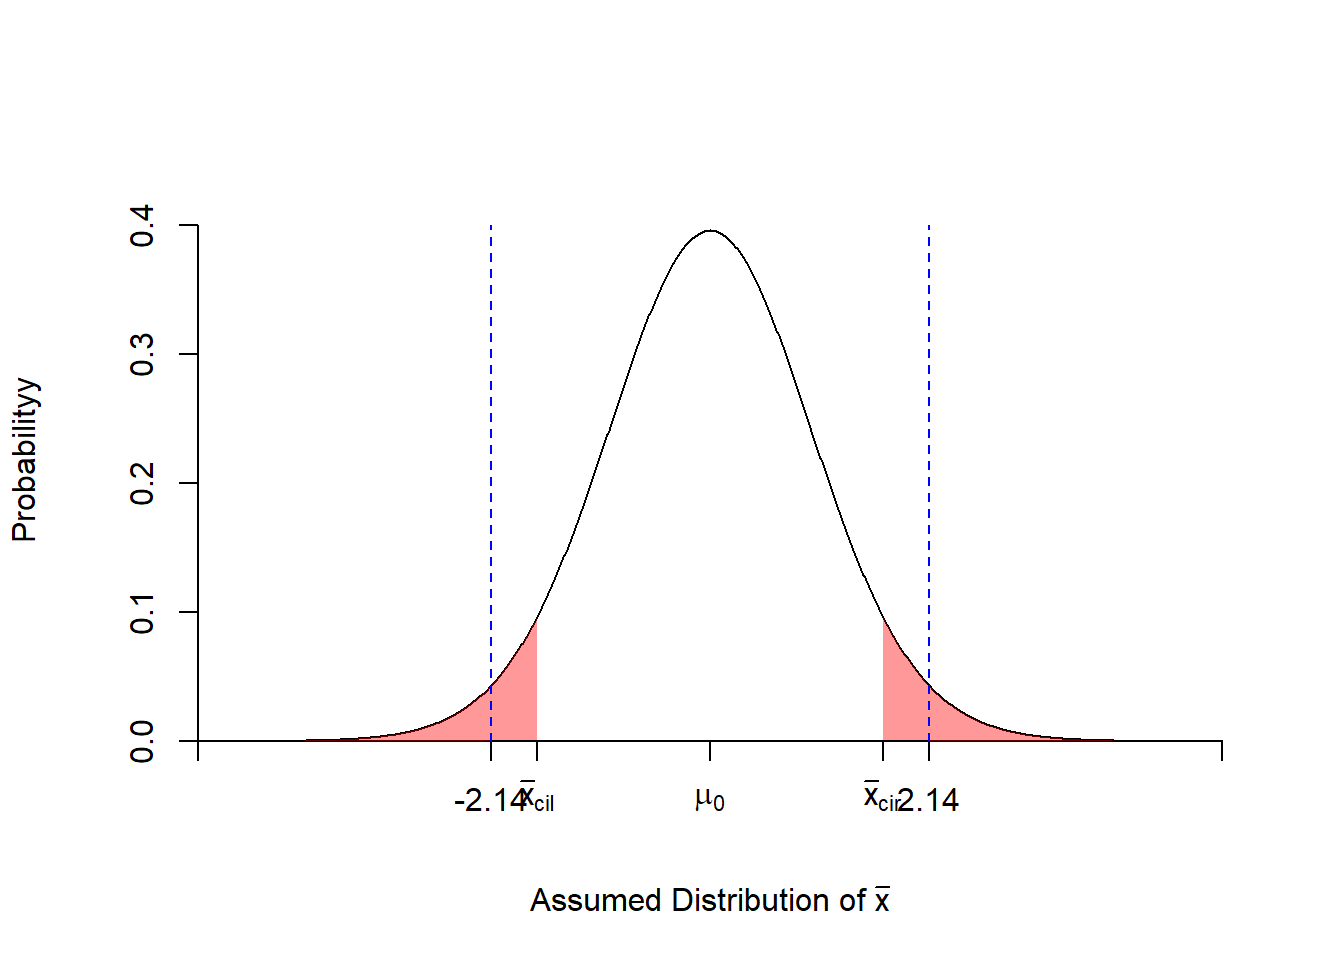
\includegraphics[width=0.49\linewidth,height=0.49\textheight]{figs/hometdist} 

}

\caption{血红蛋白样本的单样本t检验}\label{fig:hometdist}
\end{figure}

\hypertarget{ux914dux5bf9ux6837ux672ctux68c0ux9a8c}{%
\subsubsection{\texorpdfstring{配对样本\emph{t}检验}{配对样本t检验}}\label{ux914dux5bf9ux6837ux672ctux68c0ux9a8c}}

简称配对\emph{t}检验(Paired/matched \emph{t}-test),也称成对\emph{t}检验(注意区别于成组\emph{t}检验),适用于配对设计的计量资料。配对设计是将受试对象按照某些重要特征特征配成对子,再见没对中的
两个受试对象随机分配到两处理组。常见的配对设计主要有:

\begin{enumerate}
\def\labelenumi{\arabic{enumi}.}
\item
  两通志受试对象配成对子,分别接受两种不同的处理;
\item
  同一受试对象分别接受两种不同处理;
\item
  同一受试对象接受一种处理前后。
\end{enumerate}

使用《医学统计学》中的 案例3-6 的数据在R中进行配对样本\emph{t}检验测试,案例3-6属于第2种配对设计情况。

\begin{Shaded}
\begin{Highlighting}[]
\CommentTok{#使用memic包读取spss的数据格式}
\CommentTok{#install.packages('memisc')}
\KeywordTok{library}\NormalTok{(}\StringTok{"memisc"}\NormalTok{)}
\CommentTok{#读取数据}
\NormalTok{bfc_sav<-}\KeywordTok{spss.system.file}\NormalTok{(}\StringTok{"ExampleData/SavData4MedSta/Exam03-06.sav"}\NormalTok{)}
\CommentTok{#将数据形式转换为数据框}
\NormalTok{bfc_df<-}\KeywordTok{as.data.frame}\NormalTok{(}\KeywordTok{as.data.set}\NormalTok{(bfc_sav))}
\CommentTok{#直接使用t.test()进行计算,注意paired=TRUE}
\KeywordTok{t.test}\NormalTok{(bfc_df}\OperatorTok{$}\NormalTok{x1, bfc_df}\OperatorTok{$}\NormalTok{x2, }\DataTypeTok{paired=}\OtherTok{TRUE}\NormalTok{)}
\CommentTok{##  Paired t-test}
\CommentTok{## }
\CommentTok{## data:  bfc_df$x1 and bfc_df$x2}
\CommentTok{## t = 7.926, df = 9, p-value = 2.384e-05}
\CommentTok{## alternative hypothesis: true difference in means is not equal to 0}
\CommentTok{## 95 percent confidence interval:}
\CommentTok{##  0.1946542 0.3501458}
\CommentTok{## sample estimates:}
\CommentTok{## mean of the differences }
\CommentTok{##                  0.2724 }
\end{Highlighting}
\end{Shaded}

计算显示\(P=2.384e-05<\alpha=0.05\),可以认为一次抽样发生了小概率事件,因此拒绝原假设\(H_0\),
接受\(H_1\),差异有统计意义;结合案例数据意义,可认为两种方法对脂肪含量的测定结果不同,
而且第一种方法的鉴定结果数值较高(mean of the differences=0.27224 \textgreater{} 0)。

同样,可以通过绘制拒绝域和t值落点,更直观的发现t值落在左侧和右侧的拒绝域内的。

\begin{Shaded}
\begin{Highlighting}[]
\CommentTok{#l使用scales包中alpha函数改变颜色透明度}
\KeywordTok{library}\NormalTok{(}\StringTok{"scales"}\NormalTok{)}
\NormalTok{t.value<-}\FloatTok{7.926}
\NormalTok{df=}\DecValTok{9}
\NormalTok{x <-}\StringTok{ }\KeywordTok{seq}\NormalTok{(}\OperatorTok{-}\DecValTok{9}\NormalTok{,}\DecValTok{9}\NormalTok{,}\DataTypeTok{by=}\FloatTok{0.01}\NormalTok{)}
\NormalTok{y <-}\StringTok{ }\KeywordTok{dt}\NormalTok{(x,}\DataTypeTok{df=}\NormalTok{df)}
\CommentTok{#右侧p值0.95对应的t值}
\NormalTok{right <-}\StringTok{ }\KeywordTok{qt}\NormalTok{(}\FloatTok{0.95}\NormalTok{,}\DataTypeTok{df=}\NormalTok{df)}
\CommentTok{#左p值0.05对应的t值}
\NormalTok{left <-}\StringTok{ }\KeywordTok{qt}\NormalTok{(}\FloatTok{0.05}\NormalTok{,}\DataTypeTok{df=}\NormalTok{df,}\DataTypeTok{lower.tail=}\NormalTok{T)}
\CommentTok{#绘制密度曲线}
\KeywordTok{plot}\NormalTok{(x,y,}\DataTypeTok{type=}\StringTok{"l"}\NormalTok{,}\DataTypeTok{xaxt=}\StringTok{"n"}\NormalTok{,}\DataTypeTok{ylab=}\StringTok{"probabilityy"}\NormalTok{,}
     \DataTypeTok{xlab=}\KeywordTok{expression}\NormalTok{(}\KeywordTok{paste}\NormalTok{(}\StringTok{'Assumed Distribution of '}\NormalTok{,}\KeywordTok{bar}\NormalTok{(x))),}
     \DataTypeTok{axes=}\OtherTok{FALSE}\NormalTok{,}\DataTypeTok{ylim=}\KeywordTok{c}\NormalTok{(}\DecValTok{0}\NormalTok{,}\KeywordTok{max}\NormalTok{(y)}\OperatorTok{*}\FloatTok{1.1}\NormalTok{),}\DataTypeTok{xlim=}\KeywordTok{c}\NormalTok{(}\KeywordTok{min}\NormalTok{(x),}\KeywordTok{max}\NormalTok{(x)),}
     \DataTypeTok{frame.plot=}\OtherTok{FALSE}\NormalTok{)}
\CommentTok{#添加坐标轴}
\KeywordTok{axis}\NormalTok{(}\DecValTok{1}\NormalTok{,}\DataTypeTok{at=}\KeywordTok{c}\NormalTok{(}\OperatorTok{-}\DecValTok{9}\NormalTok{,left,right,}\DecValTok{0}\NormalTok{,}\DecValTok{9}\NormalTok{),}
     \DataTypeTok{pos =} \KeywordTok{c}\NormalTok{(}\DecValTok{0}\NormalTok{,}\DecValTok{0}\NormalTok{),}
     \DataTypeTok{labels=}\KeywordTok{c}\NormalTok{(}\KeywordTok{expression}\NormalTok{(}\StringTok{' '}\NormalTok{),}\KeywordTok{expression}\NormalTok{(}\KeywordTok{bar}\NormalTok{(x)[cil]),}
     \KeywordTok{expression}\NormalTok{(}\KeywordTok{bar}\NormalTok{(x)[cir]),}\KeywordTok{expression}\NormalTok{(mu[}\DecValTok{0}\NormalTok{]),}\KeywordTok{expression}\NormalTok{(}\StringTok{''}\NormalTok{)))}
\KeywordTok{axis}\NormalTok{(}\DecValTok{2}\NormalTok{,}\DataTypeTok{pos =} \KeywordTok{c}\NormalTok{(}\OperatorTok{-}\DecValTok{9}\NormalTok{,}\DecValTok{0}\NormalTok{))}
\CommentTok{#标记左侧和右侧的拒绝域}
\NormalTok{xRiReject <-}\StringTok{ }\KeywordTok{seq}\NormalTok{(right,}\DecValTok{9}\NormalTok{,}\DataTypeTok{by=}\FloatTok{0.01}\NormalTok{)}
\NormalTok{yRiReject <-}\StringTok{ }\KeywordTok{dt}\NormalTok{(xRiReject,}\DataTypeTok{df=}\NormalTok{df,)}
\NormalTok{xLeReject <-}\StringTok{ }\KeywordTok{seq}\NormalTok{(left,}\OperatorTok{-}\DecValTok{9}\NormalTok{,}\DataTypeTok{by=}\OperatorTok{-}\FloatTok{0.01}\NormalTok{)}
\NormalTok{yLeReject <-}\StringTok{ }\KeywordTok{dt}\NormalTok{(xLeReject,}\DataTypeTok{df=}\NormalTok{df)}
\CommentTok{#用poltgon()绘制拒绝域}
\KeywordTok{polygon}\NormalTok{(}\KeywordTok{c}\NormalTok{(xRiReject,xRiReject[}\KeywordTok{length}\NormalTok{(xRiReject)],xRiReject[}\DecValTok{1}\NormalTok{]),}
        \KeywordTok{c}\NormalTok{(yRiReject,}\DecValTok{0}\NormalTok{, }\DecValTok{0}\NormalTok{), }\DataTypeTok{col=}\KeywordTok{alpha}\NormalTok{(}\StringTok{"red"}\NormalTok{,}\FloatTok{0.4}\NormalTok{),}\DataTypeTok{border=}\OtherTok{NA}\NormalTok{)}
\KeywordTok{polygon}\NormalTok{(}\KeywordTok{c}\NormalTok{(xLeReject,xLeReject[}\KeywordTok{length}\NormalTok{(xLeReject)],xLeReject[}\DecValTok{1}\NormalTok{]),}
        \KeywordTok{c}\NormalTok{(yLeReject,}\DecValTok{0}\NormalTok{, }\DecValTok{0}\NormalTok{), }\DataTypeTok{col=}\KeywordTok{alpha}\NormalTok{(}\StringTok{"red"}\NormalTok{,}\FloatTok{0.4}\NormalTok{),}\DataTypeTok{border=}\OtherTok{NA}\NormalTok{)}
\CommentTok{#在坐标轴上添加t值标记}
\KeywordTok{axis}\NormalTok{(}\DecValTok{1}\NormalTok{,}\DataTypeTok{at=}\KeywordTok{c}\NormalTok{(t.value,}\OperatorTok{-}\DecValTok{1}\OperatorTok{*}\NormalTok{(t.value)),}
     \DataTypeTok{pos =} \KeywordTok{c}\NormalTok{(}\DecValTok{0}\NormalTok{,}\DecValTok{0}\NormalTok{),}\DataTypeTok{lwd.ticks=}\DecValTok{1}\NormalTok{,}
     \DataTypeTok{labels=}\KeywordTok{c}\NormalTok{( }\KeywordTok{round}\NormalTok{(t.value,}\DecValTok{2}\NormalTok{),}\KeywordTok{round}\NormalTok{(}\OperatorTok{-}\DecValTok{1}\OperatorTok{*}\NormalTok{(t.value),}\DecValTok{2}\NormalTok{)))}
\KeywordTok{arrows}\NormalTok{(}\OperatorTok{-}\DecValTok{1}\OperatorTok{*}\NormalTok{(t.value),}\DecValTok{0}\NormalTok{, }\DecValTok{-1}\OperatorTok{*}\NormalTok{(t.value), }\FloatTok{0.4}\NormalTok{, }\DataTypeTok{length =} \DecValTok{0}\NormalTok{,}\DataTypeTok{lty =}\DecValTok{2}\NormalTok{,}\DataTypeTok{col=}\StringTok{"blue"}\NormalTok{)}
\KeywordTok{arrows}\NormalTok{(t.value,}\DecValTok{0}\NormalTok{, t.value, }\FloatTok{0.4}\NormalTok{, }\DataTypeTok{length =} \DecValTok{0}\NormalTok{,}\DataTypeTok{lty =}\DecValTok{2}\NormalTok{,}\DataTypeTok{col=}\StringTok{"blue"}\NormalTok{)}
\end{Highlighting}
\end{Shaded}

\begin{figure}

{\centering 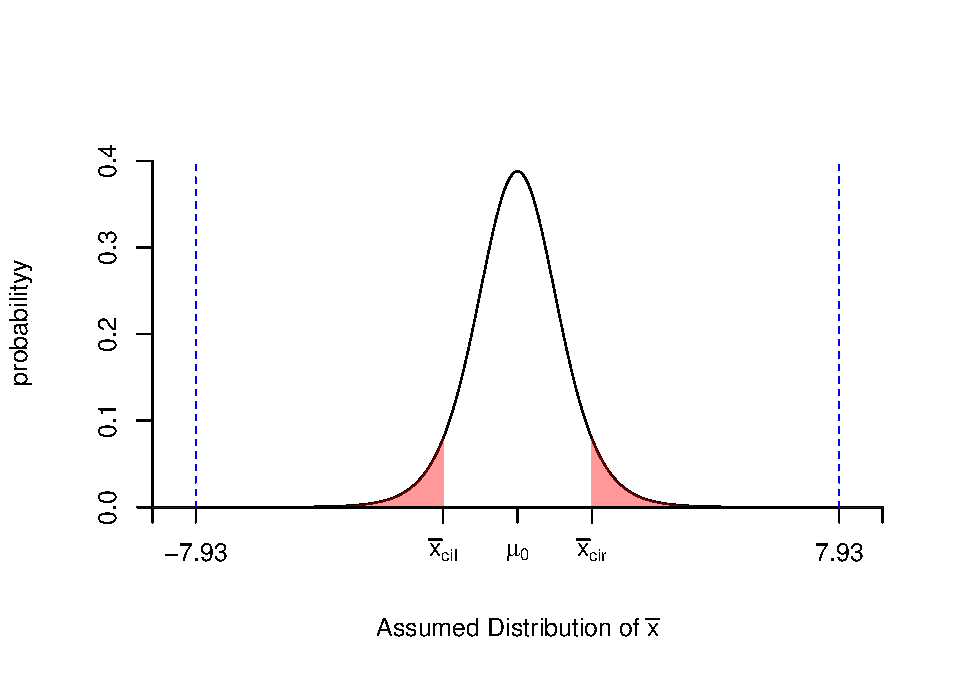
\includegraphics[width=0.49\linewidth,height=0.49\textheight]{figs/piredttest} 

}

\caption{两种方法对饮料中的脂肪含量检测的配对t检验}\label{fig:piredttest}
\end{figure}

\hypertarget{ux4e24ux79cdux72ecux7acbux6837ux672ctux68c0ux9a8c}{%
\subsubsection{两种独立样本t检验}\label{ux4e24ux79cdux72ecux7acbux6837ux672ctux68c0ux9a8c}}

两种独立样本\emph{t}检验又称为成组\emph{t}检验((Two sample/gourp \emph{t}-test),适用于完全随机设计两样本均数比较,
通常是比较两样本所代表的总体的均数是否不同。两组完全随机设计是将受试对象完全随机分配到两个不同处理组。

当两样本含量较小(\(n_1\leq60,或(和)n_2\leq60\)),且各自的总体符合正态分布(\protect\hyperlink{ux6b63ux6001ux68c0ux9a8c}{正态分布检验})时,再根据两组
数据的方差是否一样(\textbf{方差齐性},方差齐性检验)来采用不同t检验方法。

\hypertarget{ux603bux4f53ux65b9ux5deeux76f8ux7b49ux7684tux68c0ux9a8c}{%
\paragraph{\texorpdfstring{总体方差相等的\emph{t}检验}{总体方差相等的t检验}}\label{ux603bux4f53ux65b9ux5deeux76f8ux7b49ux7684tux68c0ux9a8c}}

\begin{Shaded}
\begin{Highlighting}[]
\KeywordTok{library}\NormalTok{(}\StringTok{"memisc"}\NormalTok{)}
\CommentTok{#读取数据}
\NormalTok{bfg_sav<-}\KeywordTok{spss.system.file}\NormalTok{(}\StringTok{"ExampleData/SavData4MedSta/Exam03-07.sav"}\NormalTok{)}
\CommentTok{#将数据形式转换为数据框}
\NormalTok{bfg_df<-}\KeywordTok{as.data.frame}\NormalTok{(}\KeywordTok{as.data.set}\NormalTok{(bfg_sav))}
\NormalTok{x <-}\StringTok{ }\NormalTok{bfg_df}\OperatorTok{$}\NormalTok{result[}\KeywordTok{which}\NormalTok{(bfg_df}\OperatorTok{$}\NormalTok{group}\OperatorTok{==}\DecValTok{1}\NormalTok{)]}
\NormalTok{y <-}\StringTok{ }\NormalTok{bfg_df}\OperatorTok{$}\NormalTok{result[}\KeywordTok{which}\NormalTok{(bfg_df}\OperatorTok{$}\NormalTok{group}\OperatorTok{==}\DecValTok{2}\NormalTok{)]}
\CommentTok{#直接使用t.test()进行计算,注意 var.equal=TRUE}
\KeywordTok{t.test}\NormalTok{(x,y,}\DataTypeTok{var.equal=}\OtherTok{TRUE}\NormalTok{)}

\CommentTok{##  Two Sample t-test}
\CommentTok{## }
\CommentTok{## data:  x and y}
\CommentTok{## t = -0.64187, df = 38, p-value = 0.5248}
\CommentTok{## alternative hypothesis: true difference in means is not equal to 0}
\CommentTok{## 95 percent confidence interval:}
\CommentTok{##  -2.326179  1.206179}
\CommentTok{## sample estimates:}
\CommentTok{## mean of x mean of y }
\CommentTok{##     2.065     2.625 }
\end{Highlighting}
\end{Shaded}

计算显示 \(P=0.5248>\alpha=0.05\),因此不拒绝原假设\(H_0\),差异无统计意义;结合案例数据意义,
还不能认为两种方法的预后效果不同。

\hypertarget{tux68c0ux9a8c}{%
\paragraph{\texorpdfstring{\emph{t'}检验}{t'检验}}\label{tux68c0ux9a8c}}

\emph{t'}检验,用于总体方差不相等的\emph{t}检验。当两独立小样本的均数比较,如果方差不相等(方差不齐),可采用数据变换(如两样本几何均数的\emph{t}检验,
就是将原始数据对数转换后进行\emph{t检验})处理,或采用近似\emph{t}检验(Separate variance estimation
\emph{t}-test),即\emph{t'}检验或秩转换的非参数检验,比如常用的 Cochran\&Cox法 和 Satterthwaite法 两种,
还有t.teet()里面使用的Welch法。注意的是,我了解的资料显示,似乎R语言中还没有具体实现Cochran\&Cox法
和 Satterthwaite法的函数实现,需根据公式写代码实现,可以参考下面的代码。另外,Satterthwaite法和Welch法都是在
Cochran\&Cox法的检验统计量\emph{t'}的基础上,进行的自由度矫正,然后得到矫正自由度后对应的\emph{t'}值代替\emph{t}值。

使用《医学统计学》中的 案例3-8 的数据在R中进行总体方差不相等的\emph{t}检验测试。

\begin{Shaded}
\begin{Highlighting}[]
\NormalTok{mean_x <-}\StringTok{ }\FloatTok{1.46}
\NormalTok{mean_y <-}\StringTok{ }\FloatTok{1.13}
\NormalTok{stdev_x <-}\StringTok{ }\FloatTok{1.36}
\NormalTok{stdev_y <-}\StringTok{ }\FloatTok{0.7}
\NormalTok{nx <-}\StringTok{ }\DecValTok{20}
\NormalTok{ny <-}\StringTok{ }\DecValTok{20}

\CommentTok{#Cochran&Cox法的检验统计量*t'*的}
\NormalTok{cochran_test<-}\ControlFlowTok{function}\NormalTok{(mean_x,mean_y,stdev_x,stdev_y,nx,ny) \{}
\NormalTok{  t_vul <-}\StringTok{ }\NormalTok{(mean_x}\OperatorTok{-}\NormalTok{mean_y)}\OperatorTok{/}\KeywordTok{sqrt}\NormalTok{(stdev_x}\OperatorTok{^}\DecValTok{2}\OperatorTok{/}\NormalTok{nx}\OperatorTok{+}\NormalTok{stdev_y}\OperatorTok{^}\DecValTok{2}\OperatorTok{/}\NormalTok{ny)}
  \KeywordTok{return}\NormalTok{(t_vul)}
\NormalTok{\}}

\CommentTok{#计算t'值}
\NormalTok{cochran_t<-}\KeywordTok{cochran_test}\NormalTok{(mean_x,mean_y,stdev_x,stdev_y,nx,ny)}
\CommentTok{## [1] 0.9648463}
\CommentTok{#计算P值}
\KeywordTok{pt}\NormalTok{(cochran_t,}\DataTypeTok{df=}\NormalTok{nx}\DecValTok{-1}\NormalTok{,}\DataTypeTok{lower.tail=}\NormalTok{F)}\OperatorTok{*}\DecValTok{2}
\CommentTok{## 0.3467427}

\CommentTok{#Satterthwaite法来矫正Cochran&Cox法的检验统计量*t'*的自由度}
\NormalTok{sattw_df<-}\ControlFlowTok{function}\NormalTok{(stdev_x,stdev_y,nx,ny)\{}
\NormalTok{  satt_df<-(stdev_x}\OperatorTok{^}\DecValTok{2}\OperatorTok{/}\NormalTok{nx}\OperatorTok{+}\NormalTok{stdev_y}\OperatorTok{^}\DecValTok{2}\OperatorTok{/}\NormalTok{ny)}\OperatorTok{^}\DecValTok{2}\OperatorTok{/}
\StringTok{  }\NormalTok{(((stdev_x}\OperatorTok{^}\DecValTok{2}\OperatorTok{/}\NormalTok{nx)}\OperatorTok{^}\DecValTok{2}\OperatorTok{/}\NormalTok{(nx}\DecValTok{-1}\NormalTok{))}\OperatorTok{+}
\StringTok{  }\NormalTok{((stdev_y}\OperatorTok{^}\DecValTok{2}\OperatorTok{/}\NormalTok{ny)}\OperatorTok{^}\DecValTok{2}\OperatorTok{/}\NormalTok{(ny}\DecValTok{-1}\NormalTok{)))}
  \KeywordTok{return}\NormalTok{(satt_df)}
\NormalTok{\}}
\NormalTok{satt_df<-}\KeywordTok{sattw_df}\NormalTok{(stdev_x,stdev_y,nx,ny)}
\CommentTok{#这里注意的是cochran_t>0,我们要计算cochran_t相关的双侧拒绝域面积,需要指定 lower.tail=F,并加倍}
\KeywordTok{pt}\NormalTok{(cochran_t,satt_df,}\DataTypeTok{lower.tail=}\NormalTok{F)}\OperatorTok{*}\DecValTok{2}
\CommentTok{#[1] 0.3427644}

\CommentTok{#Welch法来矫正Cochran&Cox法的检验统计量*t'*的自由度}
\NormalTok{welch_df<-}\ControlFlowTok{function}\NormalTok{(stdev_x,stdev_y,nx,ny)\{}
\NormalTok{  welch_df<-(stdev_x}\OperatorTok{^}\DecValTok{2}\OperatorTok{/}\NormalTok{nx}\OperatorTok{+}\NormalTok{stdev_y}\OperatorTok{^}\DecValTok{2}\OperatorTok{/}\NormalTok{ny)}\OperatorTok{^}\DecValTok{2}\OperatorTok{/}
\StringTok{  }\NormalTok{(((stdev_x}\OperatorTok{^}\DecValTok{2}\OperatorTok{/}\NormalTok{nx)}\OperatorTok{^}\DecValTok{2}\OperatorTok{/}\NormalTok{(nx}\OperatorTok{+}\DecValTok{1}\NormalTok{))}\OperatorTok{+}
\StringTok{  }\NormalTok{((stdev_y}\OperatorTok{^}\DecValTok{2}\OperatorTok{/}\NormalTok{ny)}\OperatorTok{^}\DecValTok{2}\OperatorTok{/}\NormalTok{(ny}\OperatorTok{+}\DecValTok{1}\NormalTok{)))}\OperatorTok{-}\DecValTok{2}
  \KeywordTok{return}\NormalTok{(welch_df)}
\NormalTok{\}}
\NormalTok{wel_df<-}\KeywordTok{welch_df}\NormalTok{(stdev_x,stdev_y,nx,ny)}
\KeywordTok{pt}\NormalTok{(cochran_t,wel_df,}\DataTypeTok{lower.tail=}\NormalTok{F)}\OperatorTok{*}\DecValTok{2}
\CommentTok{#[1] 0.3424925}
\end{Highlighting}
\end{Shaded}

从上面的计算过程可知,三种\emph{t'}检验显示了都不拒绝原假设\(H_0\),可以认为差异物统计学意义,尚不能认为两种药物
对患者的干预效果不同。但是三种发放给出的效能是不一样的,其中Welch法的最小,Cochran\&Cox法的最大,也就是说
Cochran\&Cox法更为保守。

\hypertarget{ux53c2ux6570ux4f30ux8ba1ux4e0eux5047ux8bbeux68c0ux9a8cux7684ux8054ux7cfb}{%
\paragraph{参数估计与假设检验的联系}\label{ux53c2ux6570ux4f30ux8ba1ux4e0eux5047ux8bbeux68c0ux9a8cux7684ux8054ux7cfb}}

可信区间与假设检验的区别和联系可信区间用于说明量的大小即推断总体参数(如总体均数)的范围,而假设检验用于推断
质的不同即判断两总体参数是否不等。两者既相互联系,又有区别。

一方面,可信区间亦可回答假设检验的问题,算得的可信区间若包含了\(H_0\)则按检验水准a,不拒绝\(H_0\):若不包含\(H_0\),则按检验水准a,拒绝\(H_0\),接受\(H_1\)。

另一方面,可信区间不但能回答差别是否有统计学意义,而且还能提供比假设检验更多的信息,即提示差別有无实际的专业意义。'
Figure 3.8中的 a b c 均有统计学意义(因可信区间未包含\(H_0\))。但其中:a提示有实际的专业意义(因可信区间高于有实际专业意义的值),
值得重视:b提示可能有实际专业意义;c提示无实际专业意义,该图中d、e提示差异均无统计学意义,但其中:
d因可信区间较宽,样本含量过小,抽样误差太大,难于得出结论;e提示以决策的观点,可``接受''\(H_0\),因为即使增加
样本含量,得到差异有统计学意义义,也无实际专业意义。

\begin{figure}

{\centering 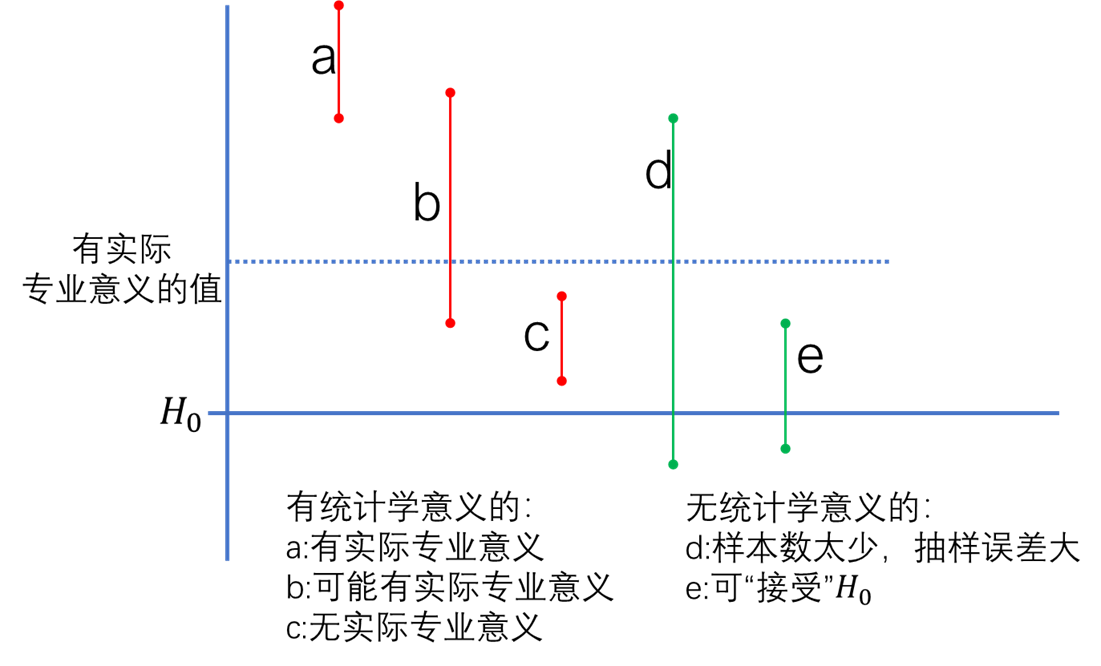
\includegraphics[width=0.49\linewidth,height=0.49\textheight]{image/ieandht} 

}

\caption{参数估计与假设检验的联系}\label{fig:Ieandht}
\end{figure}

\hypertarget{ux4e24ux6837ux672cux65b9ux5deeux9f50ux6027ux68c0ux9a8c}{%
\subsubsection{两样本方差齐性检验}\label{ux4e24ux6837ux672cux65b9ux5deeux9f50ux6027ux68c0ux9a8c}}

前面已经提到,在进行两样本检验尤其是两小样本均数的比较时,要求相应的两总体均服从正态分布且两总体方差相等,即方差齐性:
而配对,检验则要求每对数据差值的总体服从正态分布即可。因此进行两小样本检验时,一般应先对资料进行方差齐性检验Hmogeneity of variance test),
特别是发现两样本方差相差悬殊时,要判断两样本所代表的两总体方差是否不等。若方差齐,采用一般的\emph{t}检验;若方差不齐,
则采用近似\emph{t}检验(如Cochran\&Cox 的检验等)。必要时,也可对资料进行 \protect\hyperlink{ux6b63ux6001ux68c0ux9a8c}{正态性检验(Normality test)},但正态性检
验更多用于采用正态分布法制定参考值范围时。

两总体方差是否不等的判断过去多采用\emph{F}检验(\emph{F}-test),由于该检验理论上要求资料服从正态分布,但很多资料方差不齐时,
往往不服从正态分布。因此,近年来多采用更为稳健,不依赖总体分布具体形式Levene检验(Levene's test,1960)。
Levene检验实质上是将原始观测值\(X_{ij}\)转换为相应的离差\(z_{ij}\)(有多种去可选),
然后再作\href{https://zh.wikipedia.org/zh/\%E6\%96\%B9\%E5\%B7\%AE\%E5\%88\%86\%E6\%9E\%90}{方差分析},
它既可用于对两个总体方差进行齐性检验,也可用于对个总体方差进行齐性检验。这里仅介绍两样本方差比较的\emph{F}检验。

\emph{F}检验与前面介绍到的利用正态分布进行Z检验,利用\emph{t}分布进行\emph{t}检验一样,它是利用\emph{F}分布来进行检验的。
在R中,\emph{F}分布同样拥有与正态分布,\emph{t}分布类似的几个函数,分别是\href{https://stat.ethz.ch/R-manual/R-devel/library/stats/html/Fdist.html}{df(),pf(),qf()和rf()},
不过\emph{F}分布主要收两组样品的自由度共同影响。R中用\emph{F}检验来比较两组样本方差的函数是\href{https://www.rdocumentation.org/packages/stats/versions/3.6.2/topics/var.test}{var.test()}。

注意的是,方差齐性检验中的第一类错误的控制水准一般选择0.1,即\(\alpha=0.1\),而且一般约定取较大的方差作为分子,较小的方差作为分母,
这样计算出来的{[}公式{]},缩小了范围,这样可以方便查表做出结论。

使用《医学统计学》中的 案例3-6 和 案例3-8 的数据在R中进行总体方差齐性检验测试。

\begin{Shaded}
\begin{Highlighting}[]
\CommentTok{##案例3-6 }
\KeywordTok{library}\NormalTok{(}\StringTok{"memisc"}\NormalTok{)}
\CommentTok{#读取数据}
\NormalTok{bfc_sav<-}\KeywordTok{spss.system.file}\NormalTok{(}\StringTok{"ExampleData/SavData4MedSta/Exam03-06.sav"}\NormalTok{)}
\NormalTok{bfc_df<-}\KeywordTok{as.data.frame}\NormalTok{(}\KeywordTok{as.data.set}\NormalTok{(bfc_sav))}
\NormalTok{x <-}\StringTok{ }\NormalTok{bfg_df}\OperatorTok{$}\NormalTok{result[}\KeywordTok{which}\NormalTok{(bfg_df}\OperatorTok{$}\NormalTok{group}\OperatorTok{==}\DecValTok{1}\NormalTok{)]}
\NormalTok{y <-}\StringTok{ }\NormalTok{bfg_df}\OperatorTok{$}\NormalTok{result[}\KeywordTok{which}\NormalTok{(bfg_df}\OperatorTok{$}\NormalTok{group}\OperatorTok{==}\DecValTok{2}\NormalTok{)]}
\KeywordTok{var.test}\NormalTok{(x,y)}
\CommentTok{##  F test to compare two variances}
\CommentTok{## }
\CommentTok{## data:  x and y}
\CommentTok{## F = 1.5984, num df = 19, denom df = 19, p-value = 0.3153}
\CommentTok{## alternative hypothesis: true ratio of variances is not equal to 1}
\CommentTok{## 95 percent confidence interval:}
\CommentTok{##  0.6326505 4.0381795}
\CommentTok{## sample estimates:}
\CommentTok{## ratio of variances }
\CommentTok{##           1.598361 }

\CommentTok{##方法2}
\CommentTok{#用F公式来计算F值}
\NormalTok{f_val1<-}\KeywordTok{var}\NormalTok{(x)}\OperatorTok{/}\KeywordTok{var}\NormalTok{(y)}
\CommentTok{## [1] 1.598361}
\NormalTok{p_val1 <-}\StringTok{ }\KeywordTok{pf}\NormalTok{(f_val1, }\DataTypeTok{df1=}\KeywordTok{length}\NormalTok{(x)}\OperatorTok{-}\DecValTok{1}\NormalTok{, }\DataTypeTok{df2=}\KeywordTok{length}\NormalTok{(y)}\OperatorTok{-}\DecValTok{1}\NormalTok{, }\DataTypeTok{lower.tail=}\OtherTok{FALSE}\NormalTok{)}\OperatorTok{*}\DecValTok{2}
\CommentTok{## [1] 0.3152554}
\CommentTok{#将分子分母调换,需要注意lower.tail=TRUE/FALSE的设定}
\KeywordTok{pf}\NormalTok{(}\KeywordTok{var}\NormalTok{(y)}\OperatorTok{/}\KeywordTok{var}\NormalTok{(x), }\DataTypeTok{df1=}\KeywordTok{length}\NormalTok{(y)}\OperatorTok{-}\DecValTok{1}\NormalTok{, }\DataTypeTok{df2=}\KeywordTok{length}\NormalTok{(x)}\OperatorTok{-}\DecValTok{1}\NormalTok{, }\DataTypeTok{lower.tail=}\OtherTok{TRUE}\NormalTok{)}\OperatorTok{*}\DecValTok{2}

\CommentTok{##案例3-8}
\NormalTok{mean_x <-}\StringTok{ }\FloatTok{1.46}
\NormalTok{mean_y <-}\StringTok{ }\FloatTok{1.13}
\NormalTok{stdev_x <-}\StringTok{ }\FloatTok{1.36}
\NormalTok{stdev_y <-}\StringTok{ }\FloatTok{0.7}
\NormalTok{nx <-}\StringTok{ }\DecValTok{20}
\NormalTok{ny <-}\StringTok{ }\DecValTok{20}
\CommentTok{#根据F分布公式,计算F值}
\NormalTok{f_val<-stdev_x}\OperatorTok{^}\DecValTok{2}\OperatorTok{/}\NormalTok{stdev_y}\OperatorTok{^}\DecValTok{2}
\CommentTok{## [1] 3.774694}
\NormalTok{p_val <-}\StringTok{ }\KeywordTok{pf}\NormalTok{(f_val, }\DataTypeTok{df1=}\NormalTok{nx}\DecValTok{-1}\NormalTok{, }\DataTypeTok{df2=}\NormalTok{ny}\DecValTok{-1}\NormalTok{, }\DataTypeTok{lower.tail=}\OtherTok{FALSE}\NormalTok{)}\OperatorTok{*}\DecValTok{2}
\CommentTok{## [1] 0.005732012}
\end{Highlighting}
\end{Shaded}

根据计算结果,案例3-6的P值 0.3153\textgreater0.1,按照α=0.1的水准,不拒绝\(H_0\),差异不具有统计学意义,两组数据的方差相等,应该采用经典的\emph{t}检验。
案例3-8的P值 0.0057\textless0.1,按照α=0.1的水准,拒绝\(H_0\),差异具有统计学意义,两组数据的方差不相等,应该采用\emph{t'}检验。

\hypertarget{ux53d8ux91cfux8f6cux6362}{%
\subsection{变量转换}\label{ux53d8ux91cfux8f6cux6362}}

在主要的处理以前对数据进行的一些预处理,比如数据清洗,数据整合,数据变换)等。这里主要关注统计背景下的数据转换
(Transformation),也叫变量转换,从更广泛的意义上讲,变量转换是一种更改分布或关系的形状的替换。

实际资料若不满足正态性或(和)方差齐性的假定,尤其是小样本资料时,如用一般的,检验可能会导致偏离真实结果较远。
对于明显偏离上述应用条件的资料,可通过变量变换的方法加以改善。所谓变量变换(Variable transformation)是将原始
数据作某种函数转换,如转换为对数值等。它可使各组方差齐同, 亦可使偏态資料正态化,以满足,检验或其他统计分析方法对
资料的要求。通常情况下,适当的变显变换可同时达到上述两个目的。但变量变换后,在结果解释上不如原始观测变量直观,
比如地震震级是能量释放的数据的对数转换的结果,但是震级每相差1.0级,能量相差大约32倍;
每相差2.0级,能量相差约1000倍!

常用的变量变换有:

\begin{enumerate}
\def\labelenumi{\arabic{enumi}.}
\tightlist
\item
  对数变换(Logarithm)
\item
  平方根变换(Square root)
\item
  平方根反正弦变换(Arcsine, Arcsine-square)
\item
  倒数变换(Reciprocal)
\item
  指数变换(Exponential)
\end{enumerate}

其他的(如立方根等)应根据资料性质选择适当的变量变换方法。

\begin{center}\rule{0.5\linewidth}{0.5pt}\end{center}

关于变量转换的困惑?

转换的主要动机是更易于描述会和挖掘数据信息。 尽管转换的处理看起来不太自然,但这在很大程度上是心理上的反对。
拥有丰富的转换经验后会减少这种感觉,因为转换通常效果很好。 实际上,许多熟悉的测量单位也是转换后的数据,比如分贝,
pH和地震震级的里氏标度都是为对数转换后的数据。但是,在经验丰富的数据分析人员中,转换也引起了争论。
有些人经常使用它们,其他人则少得多。

所有观点都是可以辩驳的,或者至少是可以理解的。

\begin{center}\rule{0.5\linewidth}{0.5pt}\end{center}

常用的变量变换及其适用的数据分布,或者可以参考示例图\ref{fig:Datatransfromsuit}:

\begin{enumerate}
\def\labelenumi{\arabic{enumi}.}
\tightlist
\item
  变换前数据分布,集中前面, 使用倒数变换(Reciprocal);
\item
  变换前数据分布,偏前, 使用对数变换(Logarithm)
\item
  变换前数据分布,偏中前的, 使用平方根变换(Square root)
\item
  变换前数据分布,偏中后, 使用平方变换(Square),或平方根反正弦变换(Arcsine, Arcsine-square)
\item
  变换前数据分布,偏后, 使用指数变换(Exponential)
\item
  变换前,数据接近正态分布, 直接标准化
\end{enumerate}

\begin{figure}

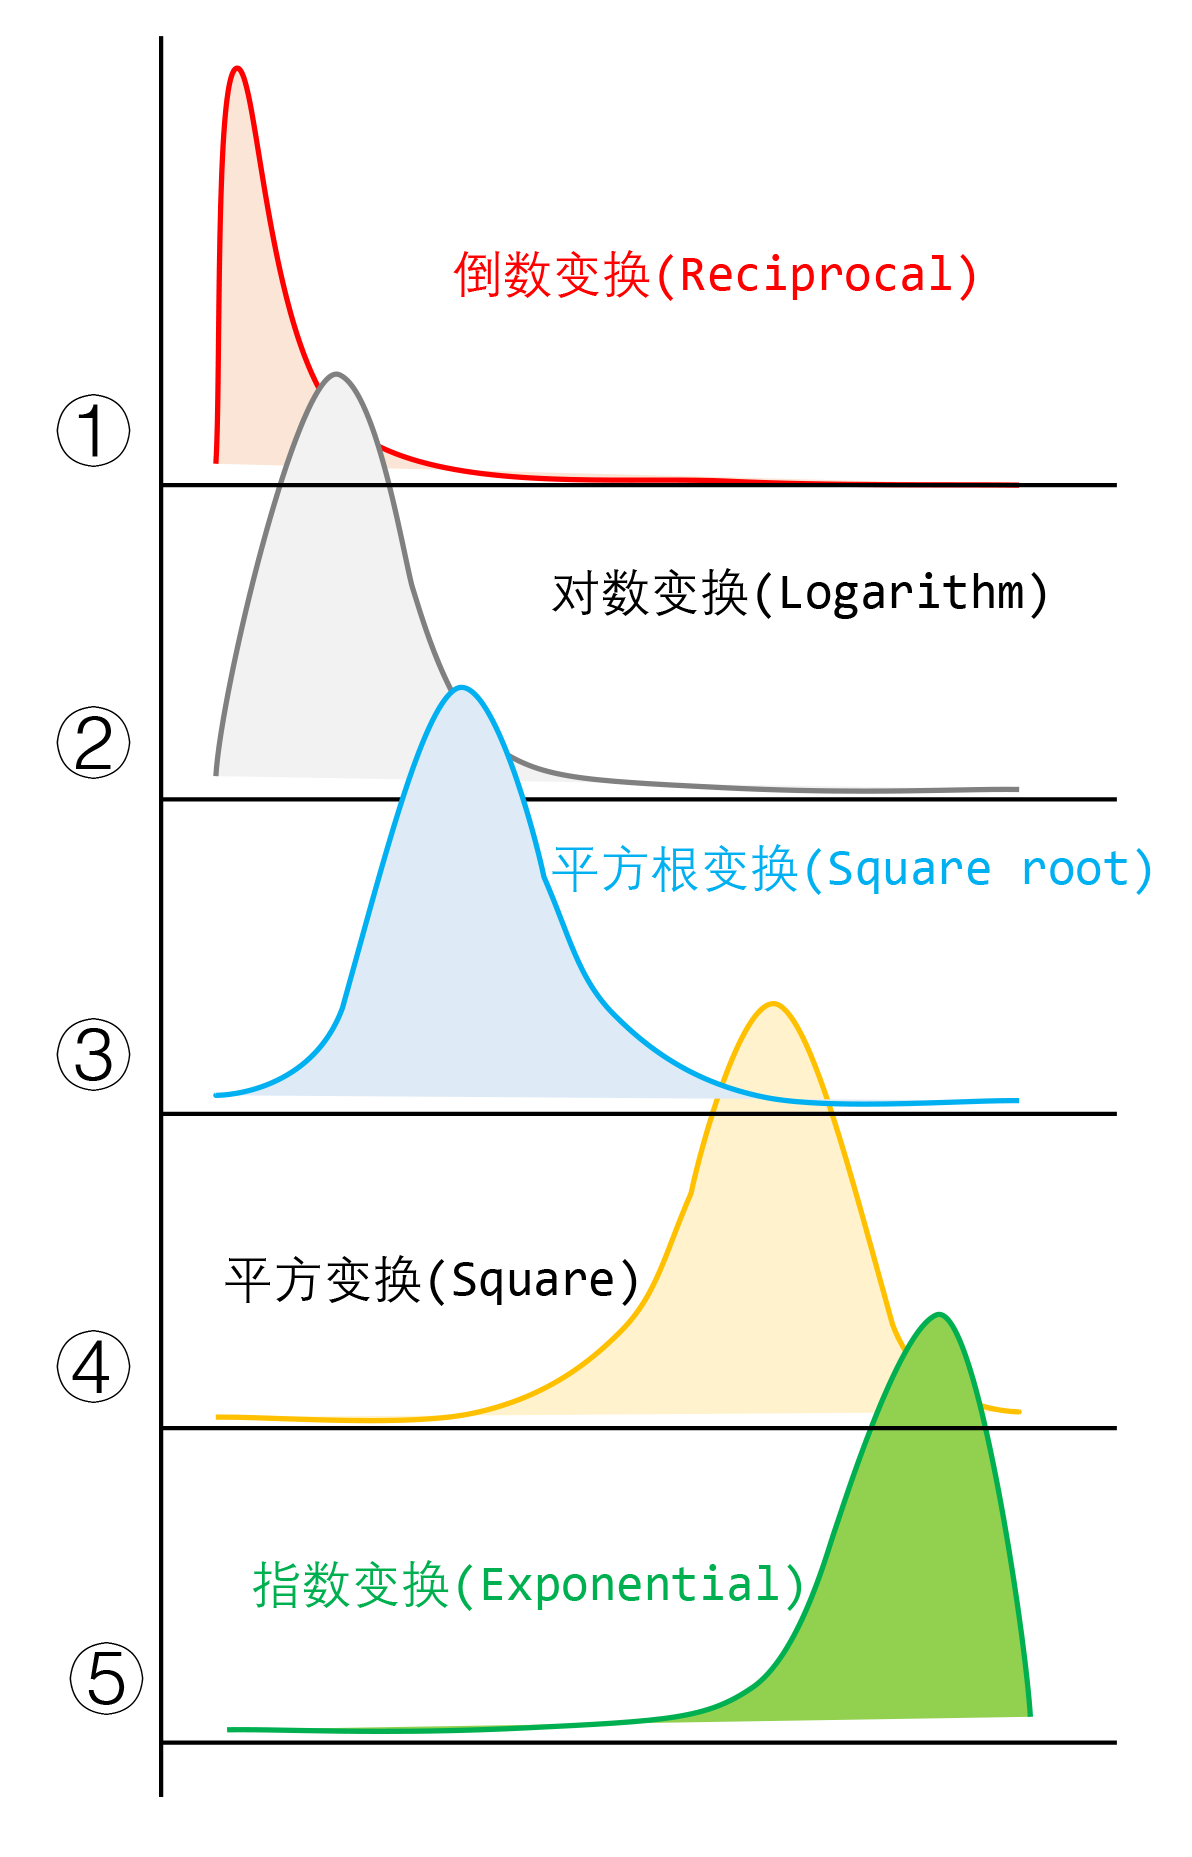
\includegraphics[width=0.5\linewidth,height=0.5\textheight]{image/Datatransfromsuit} 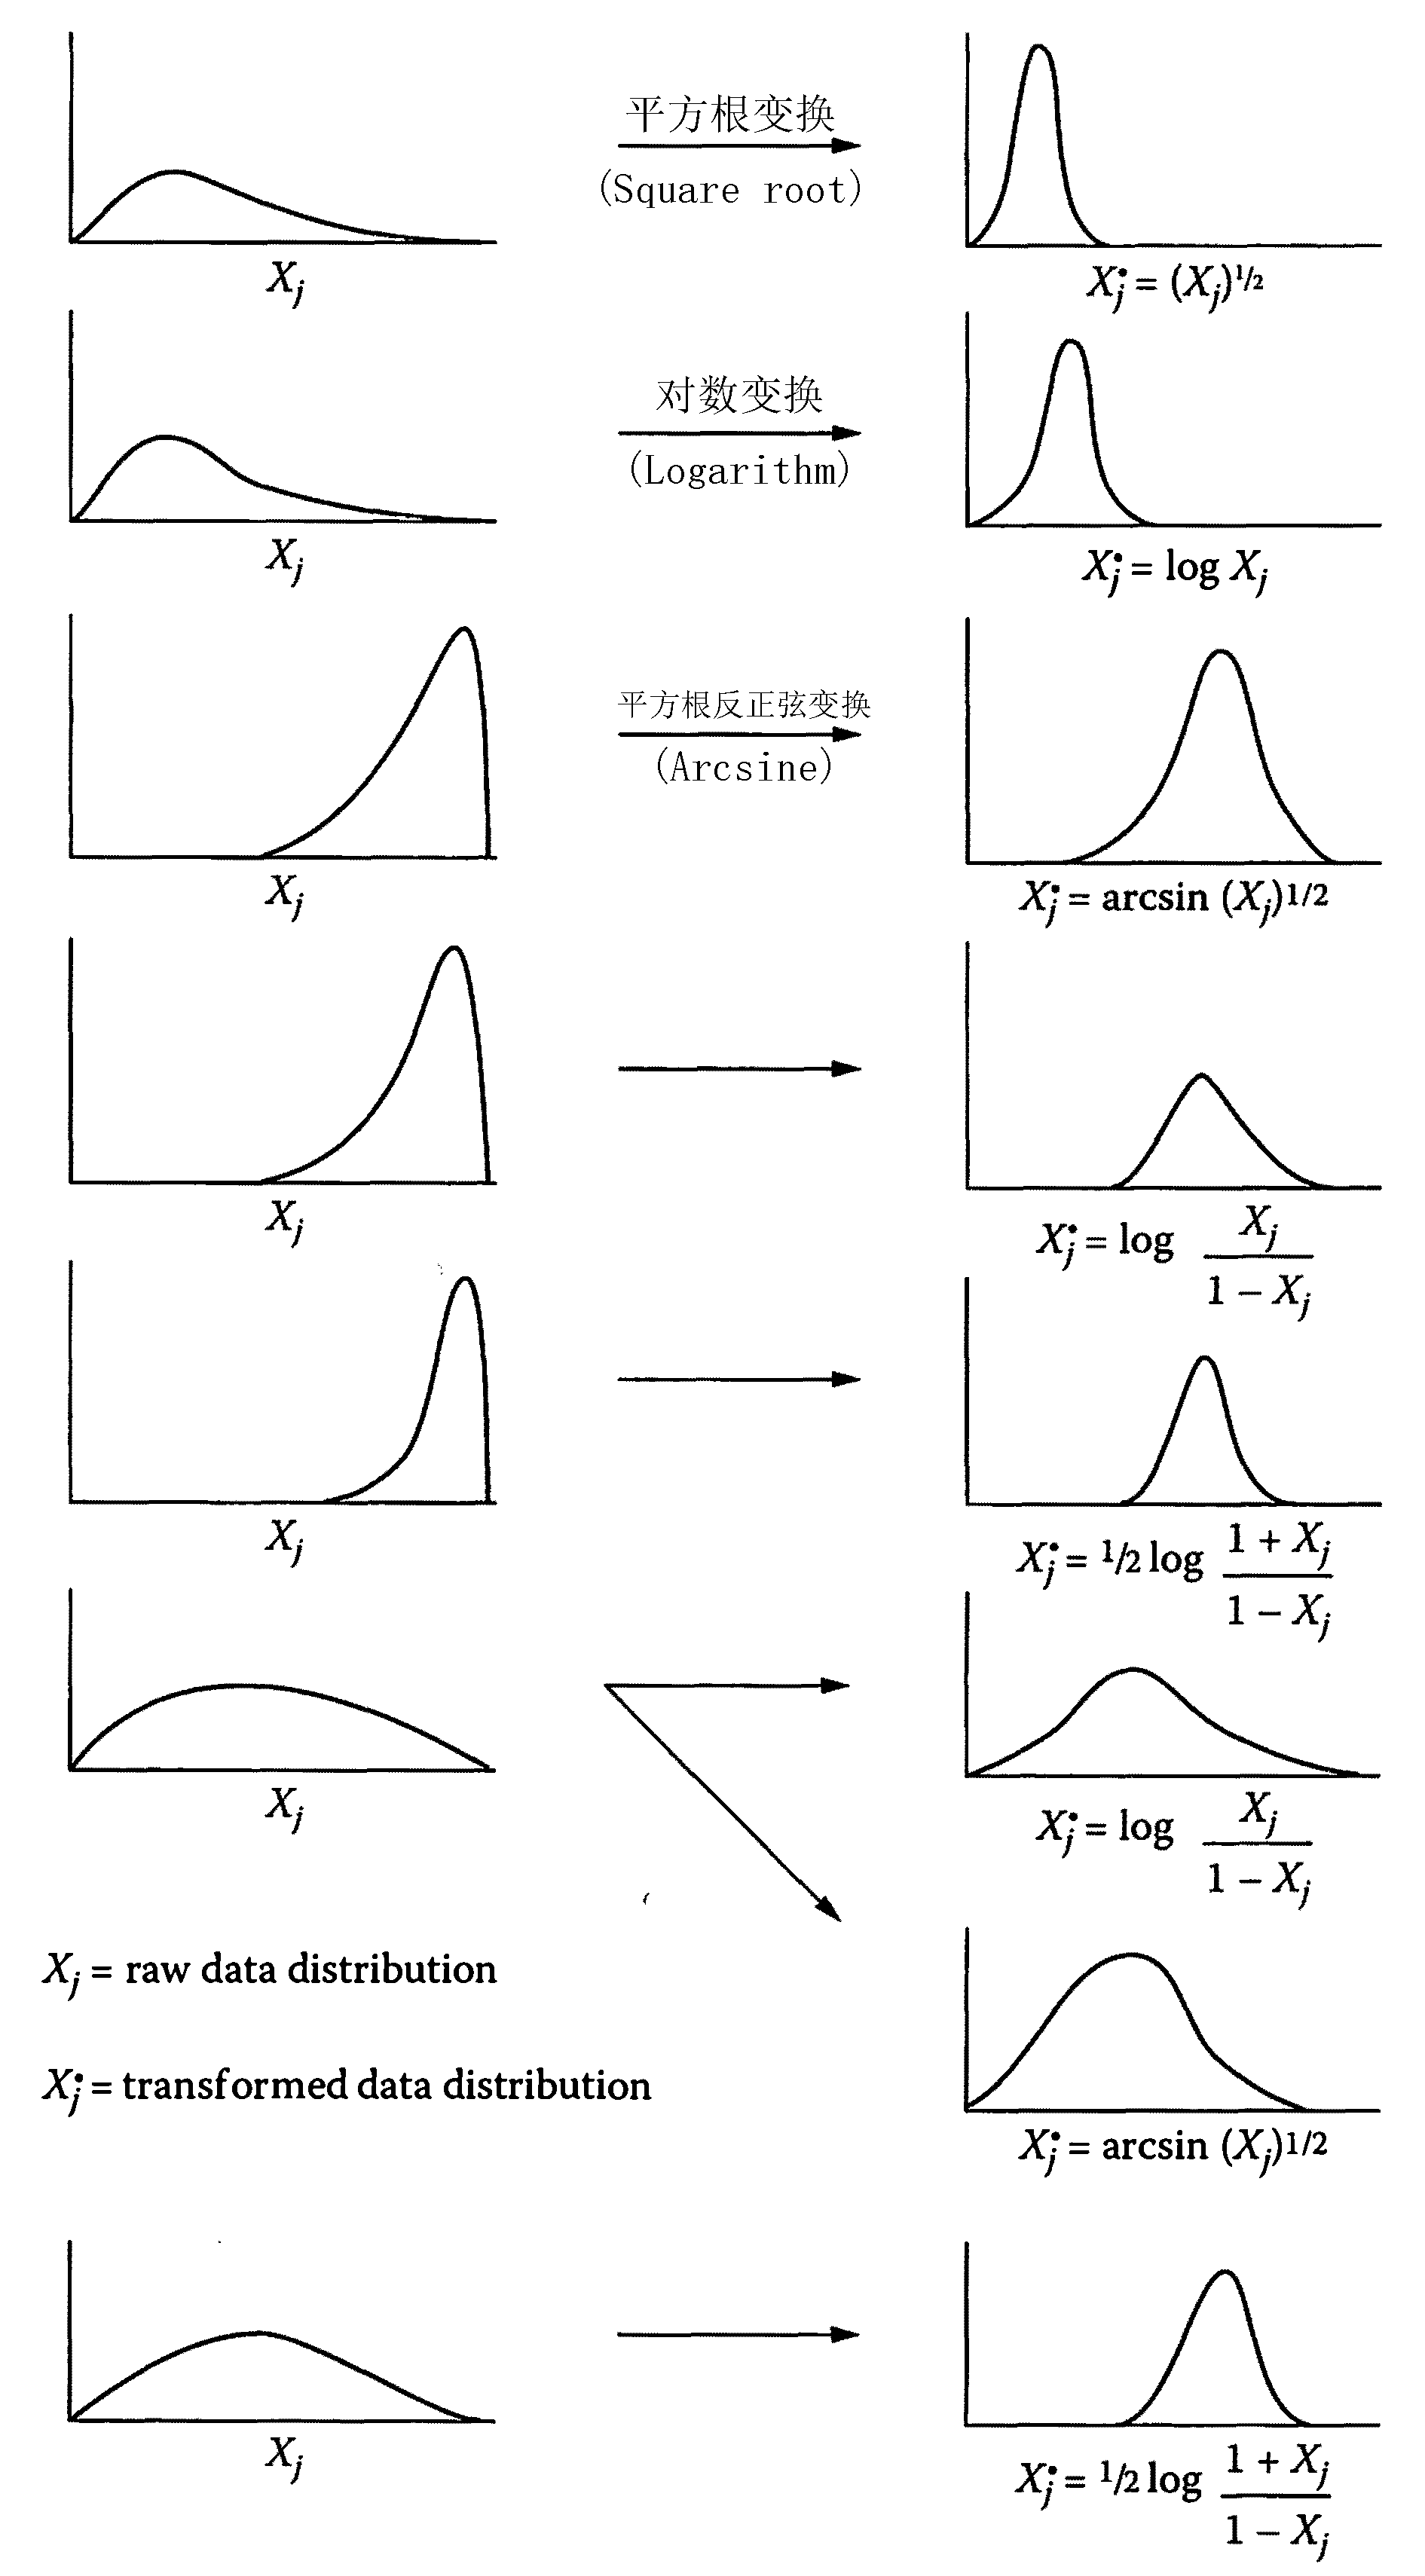
\includegraphics[width=0.5\linewidth,height=0.5\textheight]{image/Distributional transformations} \hfill{}

\caption{不同转换数据大致适应的数据分布情况, 右图来自Stevens J P. Applied multivariate statistics for the social sciences[M]. Routledge, 2012.}\label{fig:Datatransfromsuit}
\end{figure}

下面以介绍最常用的 对数变换做一个比较详细的示例,其他转换的逻辑是相同的,只是具体形式有所差别罢,故不累述。

\hypertarget{ux5bf9ux6570ux53d8ux6362}{%
\subsubsection{对数变换}\label{ux5bf9ux6570ux53d8ux6362}}

对数是指对变量x的作10,或者2,或者自然对数e 为底的对数,对分布形状有很大影响的强变换。
它通常用于减少右偏斜,并且通常适用于测量变量(一般是正态分布的连续型资料),不能应用于零或负值。 对数刻度上的一个单
位表示与所使用的对数的底数相乘,数增长或下降。

对数变换适用于: ①对数正态分布资料,即原始数据的效应是相乘时,如抗体滴度;食品、蔬菜、水果
中农药的残留量;环境中某些有毒有害物质的含量;某些疾病的潜伏期等资料;②各样本标准差与均数成
比例或变异系数是常数或接近某一常数的资料。基本形式有:

\[ X'= \lg X \]

\[X'= \lg(X+K) , (当原始数据较小或有0值时,k=1;K还可以是负数)\]

在R中进行日志记录的基本方法是使用log()函数,格式为log(value,base),
该函数返回以base为底的value的对数。 默认情况下,此函数产生自然对数值(即默认base=e)。以2为底和以10为底的函数分别为log2(),log10()。

下面是单样本数据的对数转换示例:

\begin{Shaded}
\begin{Highlighting}[]
\CommentTok{#install.packages("openintro","e1071","pryr")}
\CommentTok{#使用mammals数据集测试}
\KeywordTok{library}\NormalTok{(openintro)}
\CommentTok{#e1071包中的skewness()计算偏斜度}
\KeywordTok{library}\NormalTok{(e1071)}
\CommentTok{#使用pryr包中的绘图对象保存方案}
\KeywordTok{library}\NormalTok{(pryr)}
\KeywordTok{skewness}\NormalTok{(mammals}\OperatorTok{$}\NormalTok{body_wt)}
\CommentTok{#使用log()对body_wt数据进行转换}
\NormalTok{loged_bd_wt <-}\StringTok{ }\KeywordTok{log}\NormalTok{(mammals}\OperatorTok{$}\NormalTok{body_wt)}
\CommentTok{#skewness()计算偏斜度}
\KeywordTok{skewness}\NormalTok{(loged_bd_wt)}
\CommentTok{##[1] 0.1453599}

\NormalTok{p1.pryr }\OperatorTok\StringTok{ }\NormalTok{\{}
\KeywordTok{hist}\NormalTok{(mammals}\OperatorTok{$}\NormalTok{body_wt,}\DataTypeTok{breaks =} \DecValTok{200}\NormalTok{,}\DataTypeTok{freq=}\OtherTok{FALSE}\NormalTok{,}
 \DataTypeTok{xlim=}\KeywordTok{c}\NormalTok{(}\KeywordTok{min}\NormalTok{(mammals}\OperatorTok{$}\NormalTok{body_wt),}\KeywordTok{max}\NormalTok{(mammals}\OperatorTok{$}\NormalTok{body_wt)),}\DataTypeTok{main=}\StringTok{"Bodt wt. 数据分布"}\NormalTok{)}
\KeywordTok{lines}\NormalTok{(}\KeywordTok{density}\NormalTok{(mammals}\OperatorTok{$}\NormalTok{body_wt), }\DataTypeTok{col=}\StringTok{"red"}\NormalTok{, }\DataTypeTok{lwd=}\DecValTok{1}\NormalTok{)}
\NormalTok{\}}

\NormalTok{p2.pryr }\OperatorTok\StringTok{ }\NormalTok{\{}
  \KeywordTok{hist}\NormalTok{(loged_bd_wt,}\DataTypeTok{breaks =} \DecValTok{200}\NormalTok{,}\DataTypeTok{freq=}\OtherTok{FALSE}\NormalTok{,}
 \DataTypeTok{xlim=}\KeywordTok{c}\NormalTok{(}\KeywordTok{min}\NormalTok{(loged_bd_wt),}\KeywordTok{max}\NormalTok{(loged_bd_wt)),}\DataTypeTok{main=}\StringTok{"经过Log转换后Bodt wt. 数据分布"}\NormalTok{)}
\KeywordTok{lines}\NormalTok{(}\KeywordTok{density}\NormalTok{(loged_bd_wt), }\DataTypeTok{col=}\StringTok{"red"}\NormalTok{, }\DataTypeTok{lwd=}\DecValTok{1}\NormalTok{)}
\NormalTok{\}}

\KeywordTok{split.screen}\NormalTok{(}\KeywordTok{c}\NormalTok{(}\DecValTok{1}\NormalTok{, }\DecValTok{2}\NormalTok{))}
\KeywordTok{screen}\NormalTok{(}\DecValTok{1}\NormalTok{)}
\NormalTok{p1.pryr}
\KeywordTok{screen}\NormalTok{(}\DecValTok{2}\NormalTok{)}
\NormalTok{p2.pryr}
\end{Highlighting}
\end{Shaded}

\begin{figure}

{\centering 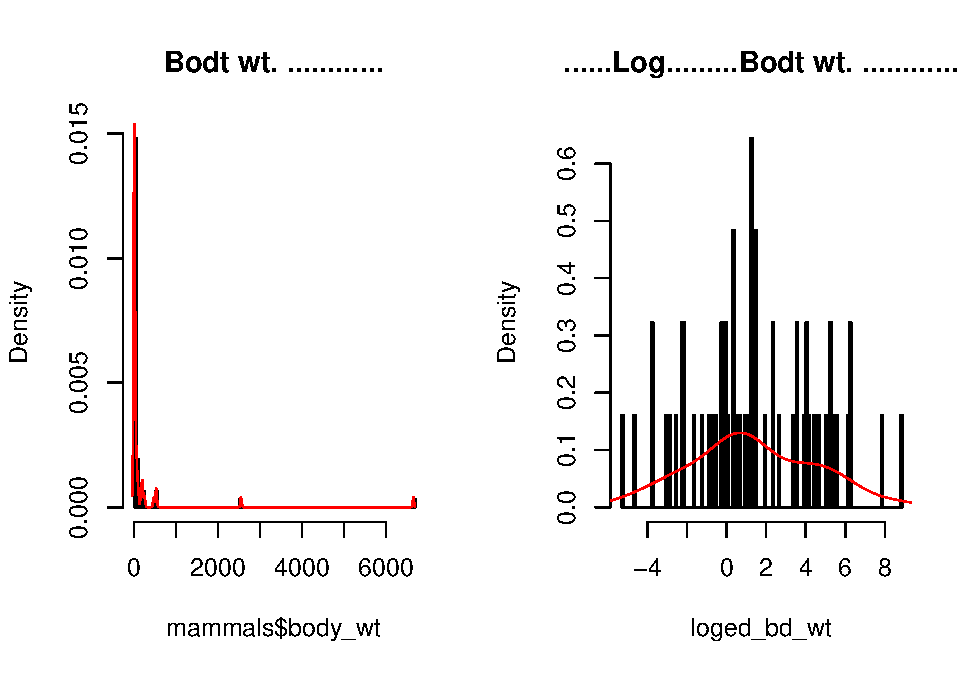
\includegraphics[width=0.9\linewidth]{figs/logtrans1} 

}

\caption{log转换前后的Mammal数据分布}\label{fig:logtrans1}
\end{figure}

下面是两组样本数据的对数转换示例,在mammals\$body\_wt数据上结合mammals\$brain\_wt数据:

\begin{Shaded}
\begin{Highlighting}[]
\CommentTok{#使用log()对brain_wt数据进行转换}
\NormalTok{loged_br_wt <-}\StringTok{ }\KeywordTok{log}\NormalTok{(mammals}\OperatorTok{$}\NormalTok{brain_wt)}
\NormalTok{p3.pryr }\OperatorTok\StringTok{ }\NormalTok{\{}
  \KeywordTok{plot}\NormalTok{(mammals}\OperatorTok{$}\NormalTok{body_wt,mammals}\OperatorTok{$}\NormalTok{brain_wt,}\DataTypeTok{main=}\StringTok{"body_wt vs brain_wt"}\NormalTok{,}\DataTypeTok{col=}\StringTok{"red"}\NormalTok{,}\DataTypeTok{pch=}\DecValTok{16}\NormalTok{)}
\NormalTok{\}}
\NormalTok{p4.pryr }\OperatorTok\StringTok{ }\NormalTok{\{}
  \KeywordTok{plot}\NormalTok{(loged_bd_wt,loged_br_wt,}\DataTypeTok{main=}\StringTok{"body_wt vs brain_wt after both loged"}\NormalTok{,}\DataTypeTok{col=}\StringTok{"red"}\NormalTok{,}\DataTypeTok{pch=}\DecValTok{16}\NormalTok{)}
\NormalTok{\}}
\KeywordTok{split.screen}\NormalTok{(}\KeywordTok{c}\NormalTok{(}\DecValTok{1}\NormalTok{, }\DecValTok{2}\NormalTok{))}
\KeywordTok{screen}\NormalTok{(}\DecValTok{1}\NormalTok{)}
\NormalTok{p3.pryr}
\KeywordTok{screen}\NormalTok{(}\DecValTok{2}\NormalTok{)}
\NormalTok{p4.pryr}
\end{Highlighting}
\end{Shaded}

\textbackslash begin\{figure\}

\{\centering 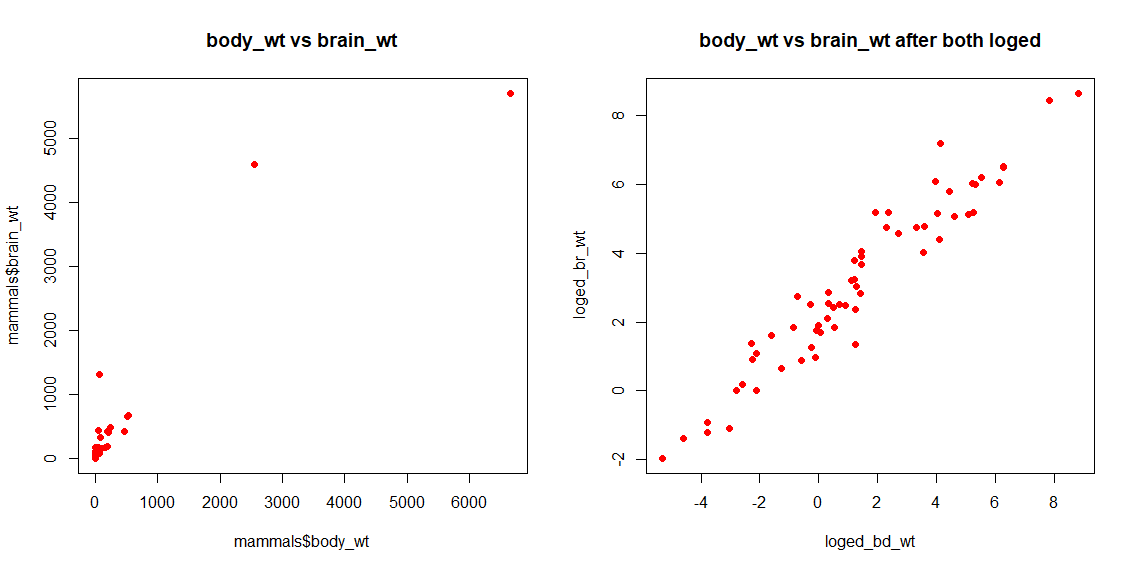
\includegraphics[width=0.99\linewidth,height=0.99\textheight]{image/badywtVSbrainwt}

\}

\textbackslash caption\{log转换前后的body\_wt vs brain\_wt\}\label{fig:bbwtlog}
\textbackslash end\{figure\}

在建立预测模型时,数据转换也可以起到很大效果。我们可以看看用mammals\$body\_wt和mammals\$brain\_wt来构建线性模型时,使用对数转换前后的残差(Residual standard error)变化。
计算结果显示,数据转换前的预测模型的残差是334.7,对数转换后的预测模型的残差是0.6943,相比转换前的要小非常多了。

\begin{Shaded}
\begin{Highlighting}[]
\NormalTok{lm.model <-}\StringTok{ }\KeywordTok{lm}\NormalTok{(mammals}\OperatorTok{$}\NormalTok{brain_wt }\OperatorTok{~}\StringTok{ }\NormalTok{mammals}\OperatorTok{$}\NormalTok{body_wt)}
\NormalTok{lm_log.model <-}\StringTok{ }\KeywordTok{lm}\NormalTok{(loged_br_wt }\OperatorTok{~}\StringTok{ }\NormalTok{loged_bd_wt)}
\KeywordTok{summary}\NormalTok{(lm.model)}
\CommentTok{## Call:}
\CommentTok{## lm(formula = mammals$brain_wt ~ mammals$body_wt)}
\CommentTok{## }
\CommentTok{## Residuals:}
\CommentTok{##     Min      1Q  Median      3Q     Max }
\CommentTok{## -810.07  -88.52  -79.64  -13.02 2050.33 }
\CommentTok{## }
\CommentTok{## Coefficients:}
\CommentTok{##                 Estimate Std. Error t value Pr(>|t|)    }
\CommentTok{## (Intercept)     91.00440   43.55258    2.09   0.0409 *  }
\CommentTok{## mammals$body_wt  0.96650    0.04766   20.28   <2e-16 ***}
\CommentTok{## ---}
\CommentTok{## Signif. codes:  0 ‘***’ 0.001 ‘**’ 0.01 ‘*’ 0.05 ‘.’ 0.1 ‘ ’ 1}
\CommentTok{## }
\CommentTok{## Residual standard error: 334.7 on 60 degrees of freedom}
\CommentTok{## Multiple R-squared:  0.8727, Adjusted R-squared:  0.8705 }
\CommentTok{## F-statistic: 411.2 on 1 and 60 DF,  p-value: < 2.2e-16}
\KeywordTok{summary}\NormalTok{(lm_log.model)}
\CommentTok{##  Call:}
\CommentTok{##  lm(formula = loged_br_wt ~ loged_bd_wt)}
\CommentTok{##  }
\CommentTok{##  Residuals:}
\CommentTok{##       Min       1Q   Median       3Q      Max }
\CommentTok{##  -1.71550 -0.49228 -0.06162  0.43597  1.94829 }
\CommentTok{##  }
\CommentTok{##  Coefficients:}
\CommentTok{##              Estimate Std. Error t value Pr(>|t|)    }
\CommentTok{##  (Intercept)  2.13479    0.09604   22.23   <2e-16 ***}
\CommentTok{##  loged_bd_wt  0.75169    0.02846   26.41   <2e-16 ***}
\CommentTok{##  ---}
\CommentTok{##  Signif. codes:  0 ‘***’ 0.001 ‘**’ 0.01 ‘*’ 0.05 ‘.’ 0.1 ‘ ’ 1}
\CommentTok{##  }
\CommentTok{##  Residual standard error: 0.6943 on 60 degrees of freedom}
\CommentTok{##  Multiple R-squared:  0.9208,    Adjusted R-squared:  0.9195 }
\CommentTok{##  F-statistic: 697.4 on 1 and 60 DF,  p-value: < 2.2e-16}
\end{Highlighting}
\end{Shaded}

\hypertarget{ux7b2cux56dbux7ae0-ux591aux4e2aux6837ux672cux5747ux6570ux6bd4ux8f83ux7684ux65b9ux5deeux5206ux6790}{%
\section{第四章 多个样本均数比较的方差分析}\label{ux7b2cux56dbux7ae0-ux591aux4e2aux6837ux672cux5747ux6570ux6bd4ux8f83ux7684ux65b9ux5deeux5206ux6790}}

日期: 2020-11-18
作者:wxhyihuan

T检验只能比较两组样本均值,对于多组的样本处理就需要用方差分析(Analysis of variance. ANOVA)。

在进行科学研究时,有时要按实验(对人称为试验)设计将所研究的对象分为多个处理组施加不同的干预(比如治疗某种疾病的方式),施加的干预为处理,
处理因素(Treatment,如用药处理,手术处理,药品剂量等)至少有两个水平(Level,比如药物种类有A,B,C三种,即为3个水平)。这类科研资料的统计分析, 是通过所获得的样本信息来推断各处理组均数
间的差别是否有统计学意义,即处理有无效果。常采用 的统计分析方法为方差分析,由英国统计学家R. A. Fisher 首创,
为纪念 Fisher.以F命名,故方差分析又称\emph{F}检验,也称为 ``变异数分析''。

\emph{F}检验与前面的\emph{t}检验或者Z检验类似,也有自己的概率分布基础,即方差分析是依靠\href{https://zh.wikipedia.org/wiki/F-\%E5\%88\%86\%E5\%B8\%83}{F-分布}为概率分布的依据,
利用离均差平方和(Sum of square of deviations from mean,SS)与自由度(Degree of freedom, df)所计算的组间与组内均方(Mean of square,MS)估计出F值和P值,结合检验水准\(\alpha=0.05\)判断检验结果。
若有统计学意义(\(P值\le0.05\)),则拒绝原假设\(H_0(μ_0=μ_1=μ_2=μ_3=\cdots)\),接受\(H_1\)(\(μ\)不完全相等),即各样本不是来自不完全相同的总体;
反之,若没有统计学意义(\(P值>0.05\)),则不拒绝原假设\(H_0(μ_0=μ_1=μ_2=μ_3=\cdots)\),即还不能确定各样本是来自不完全相同的总体;

\hypertarget{fux5206ux5e03}{%
\subsection{\texorpdfstring{\emph{F}分布}{F分布}}\label{fux5206ux5e03}}

\emph{F}分布定义是设\(X\)、\(Y\)为两个独立的随机变量,\(X\)服从自由度为k1的\href{https://zh.wikipedia.org/zh-cn/\%E5\%8D\%A1\%E6\%96\%B9\%E5\%88\%86\%E4\%BD\%88}{卡方分布},
\(Y\)服从自由度为k2的卡方分布,这两个独立的卡方分布除以各自的自由度后的比率这一统计量的分布,即服从F-分布(F-distribution),
即:
\[F=\frac{U_1/d_1}{U_2/d_2}\]
\(U_1\)和\(U_2\)分别是自由度(Degree of freedom, df)为d1和d2的卡方分布,\(U_1=\sum_{i=0}^nX_i^2\),\(U_2=\sum_{i=0}^nY_i^2\);或者
\[\frac{S_1^2/d_1}{\sigma_1^2}\div\frac{S_2^2/d_2}{\sigma_2^2}\]
\(S_1^2\)为正态分布\(N(0,\sigma_1^2)\)的\(d_1\)个随机变量的平方和,\(S_2^2\)为正态分布\(N(0,\sigma_2^2)\)的\(d_2\)个随机变量的平方和。

F-分布对应的概率密度函数是:
\[\begin{aligned}
f(x,d_1,d_2) &= \frac{\sqrt{\frac{(d_{1}x)^{d_1} d_2^{d_2}}{(d_{1}x+d_2)^{d_1+d2}}}}{xB\left(d_{1}/2,d_{2}/2\right)}\\
&= \frac{1}{B\left(d_{1}/2,d_{2}/2\right)}\left(\frac{d_1}{d_2}\right)^{\frac{d_1}{2}}x^{\frac{d_1}{2}-1}\left(1+\frac{d_1}{d_2}x\right)^{-\frac{d_1+d_2}{2}}
\end{aligned}\]

在R语言中。F-分布也有几个与Z分布,\emph{t}分布基本函数类似的工具函数,分别是\href{https://stat.ethz.ch/R-manual/R-devel/library/stats/html/Fdist.html}{df(),pf(),qf()和rf()}。

\begin{Shaded}
\begin{Highlighting}[]
\NormalTok{f_val =}\StringTok{ }\FloatTok{2.2}
\NormalTok{df1 =}\StringTok{ }\DecValTok{10}
\NormalTok{df2 =}\StringTok{ }\DecValTok{20}
\NormalTok{q_seq <-}\StringTok{ }\KeywordTok{c}\NormalTok{(}\FloatTok{0.25}\NormalTok{, }\FloatTok{0.5}\NormalTok{, }\FloatTok{0.75}\NormalTok{, }\FloatTok{0.999}\NormalTok{)}

\KeywordTok{df}\NormalTok{(f_val, }\DataTypeTok{df1 =}\NormalTok{ df1, }\DataTypeTok{df2 =}\NormalTok{ df2)}
\CommentTok{## [1] 0.007858262}
\KeywordTok{pf}\NormalTok{(f_val, }\DataTypeTok{df =}\NormalTok{ df1, }\DataTypeTok{df2 =}\NormalTok{ df2, }\DataTypeTok{lower.tail =} \OtherTok{TRUE}\NormalTok{)}
\CommentTok{## [1] 0.9944622}
\KeywordTok{qf}\NormalTok{(q_seq, }\DataTypeTok{df1 =}\NormalTok{ df1, }\DataTypeTok{df2 =}\NormalTok{ df2, }\DataTypeTok{lower.tail =} \OtherTok{TRUE}\NormalTok{)}
\CommentTok{## [1] 0.6563936 0.9662639 1.3994874 5.0752462}

\NormalTok{x <-}\StringTok{ }\KeywordTok{rf}\NormalTok{(}\DecValTok{100000}\NormalTok{, }\DataTypeTok{df1 =}\NormalTok{ df1, }\DataTypeTok{df2 =}\NormalTok{ df2)}
\KeywordTok{hist}\NormalTok{(x, }\DataTypeTok{col=}\StringTok{"#A8D6FF"}\NormalTok{,}
     \DataTypeTok{breaks =} \StringTok{'Scott'}\NormalTok{, }\DataTypeTok{freq =} \OtherTok{FALSE}\NormalTok{, }
     \DataTypeTok{xlim =} \KeywordTok{c}\NormalTok{(}\DecValTok{0}\NormalTok{,}\DecValTok{3}\NormalTok{), }\DataTypeTok{ylim =} \KeywordTok{c}\NormalTok{(}\DecValTok{0}\NormalTok{,}\DecValTok{1}\NormalTok{),}
     \DataTypeTok{xlab =} \StringTok{''}\NormalTok{, }\DataTypeTok{main =} \StringTok{'Histogram for a F-distribution with df1=10, df2=20'}\NormalTok{, }\DataTypeTok{cex.main=}\FloatTok{0.9}\NormalTok{)}

\KeywordTok{curve}\NormalTok{(}\KeywordTok{df}\NormalTok{(x, }\DataTypeTok{df1 =}\NormalTok{ df1, }\DataTypeTok{df2 =}\NormalTok{ df2), }\DataTypeTok{from =} \DecValTok{0}\NormalTok{, }\DataTypeTok{to =} \DecValTok{3}\NormalTok{, }\DataTypeTok{n =} \DecValTok{10000}\NormalTok{, }\DataTypeTok{col=} \StringTok{'red'}\NormalTok{, }\DataTypeTok{lwd=}\DecValTok{2}\NormalTok{, }\DataTypeTok{add =}\NormalTok{ T)}
\end{Highlighting}
\end{Shaded}

\begin{figure}

{\centering 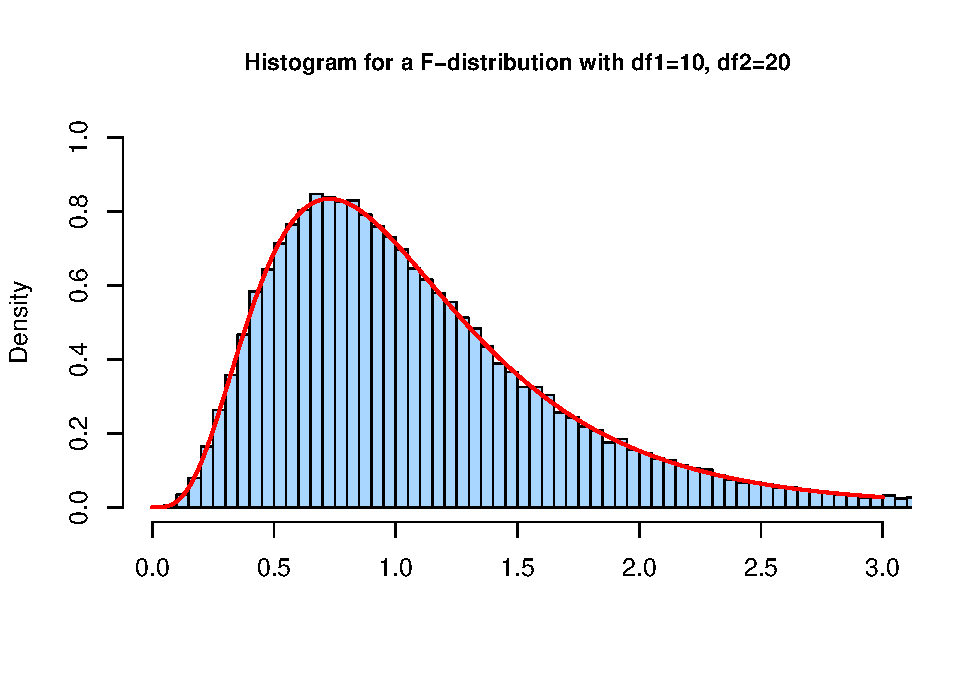
\includegraphics[width=0.49\linewidth]{figs/fdistri} 

}

\caption{F-分布的概率密度曲线测试}\label{fig:fdistri}
\end{figure}

\hypertarget{fux68c0ux9a8cux7684ux5206ux7c7bux539fux7406ux53caux5e94ux7528}{%
\subsection{\texorpdfstring{\emph{F}检验的分类、原理及应用}{F检验的分类、原理及应用}}\label{fux68c0ux9a8cux7684ux5206ux7c7bux539fux7406ux53caux5e94ux7528}}

\hypertarget{ux5206ux7c7b}{%
\subsubsection{分类}\label{ux5206ux7c7b}}

按方差分析的基本运算概念,依照所感兴趣的因子数量而可分三大类:

\begin{enumerate}
\def\labelenumi{\arabic{enumi}.}
\tightlist
\item
  单因子方差分析(One-way ANOVA)
\item
  双因子方差分析(Two-way ANOVA)
\item
  多因子方差分析(Multi-way ANOVA)
\end{enumerate}

如果依照因子的特性不同而有三种型态,分别是:

\begin{enumerate}
\def\labelenumi{\arabic{enumi}.}
\tightlist
\item
  固定效应方差分析(Fixed-effect ANOVA)
\item
  随机效应方差分析(Random-effect ANOVA)
\item
  混合效应方差分析(Mixed-effect ANOVA)
\end{enumerate}

一般的,按照因子数量的分类进行区分使用情况比较常见,这里借用单因素方差分析(One-way ANOVA)介绍方差分析的基本思想

\hypertarget{ux539fux7406}{%
\subsubsection{原理}\label{ux539fux7406}}

ANOVA通过分析方差来推断均值是否和总体有显著性差异(注意:虽然叫做方差分析,但是它的目的是检验每个组的平均数是否相同)。
ANOVA把方差分为处理因素(Treatment effect,真实差异)和误差(Error effect,抽样误差或个体差异)两个来源,两个方差的比值服从F分布,因为方差本身
就是个体和均值差平方和,所以对方差组成的分析能够反映均值的差异。处理效应(Treatment effect)是不同组的均值间的差异,误差(Error effect)是组内
个体间的差异,习惯性地称前者为组间(Between)差异,后者为组内(Wthin)差异。

例如,在工业生产或实验研究中,为了比较药物X,Y,Z对治疗某疾病的疗效,我们将实验对象分成三组,分别记录服用X,Y,Z三种药物的治疗效果,并依次得到三组样本如下:
\[\begin{aligned}
& X_1,X_2,X_3,\cdots,X_{n1};\\
& Y_1,Y_2,Y_3,\cdots,Y_{n2};\\
& Z_1,Z_2,Z_3,\cdots,Z_{n3};
\end{aligned}\]
通过这些实验数据,我们希望回答:①三种药物对治疗该疾病有没有显著差异;②如果有差异,哪种药物治疗效果最好?

这个例子中,药物称为处理因素,X,Y,Z称为该因素的水平。这个实验只涉及单个处理因素------``药物'',我们称之为单因素实验,对应的方差分析处理叫单因子方差分析(One-way ANOVA)。此外,如果比较不同的药物和
剂量对疗效的影响,这就是双因素实验,对应的方差分析叫双因子方差分析(Two-way ANOVA),由此类似可推广到多因素实验和多因子方差分析(Multi-way ANOVA)。

示例中,我们记总均数\(\bar{M}\),各分组(水平)的均数为\(\bar{X}\),\(\bar{Y}\),\(\bar{Z}\),总样本个数\(N=n_1+n_2+n_3\),
分组(水平)个数记为g,本例中g=3。
\[\bar{M}=\frac{\sum_{i=0}^{n1}X_{n1}+\sum_{i=0}^{n2}Y_{n2}+\sum_{i=0}^{n3}Z_{n3}}{n_1+n_2+n_3}\]

把所有分组的混在一起,当成一个样本,总的方差的自由度为\(v_t=N-1\),(\(SS_{tol}\)总变异)公式为:
\[\begin{aligned}
SS_{t} &= \sum_{i=1}^g\sum_{j=1}^{n_i}(X_{ij}-\bar{X})\\
 &= \sum_{i=1}^g\sum_{j=1}^{n_i}X_{ij}^2-(\sum_{i=1}^g\sum_{j=1}^{n_i}X_{ij})^2/N
\end{aligned}\]

组间方差的自由度为\(v_b=g-1\),组间方差\(SS_{b}\)为:
\[\begin{aligned}
SS_{b} &= \sum_{i=1}^gn_i(X_{i}-\bar{X})\\
 &= \sum_{i=1}^g\frac{(\sum_{j=1}^nX_{ij})^2}{n_i}-(\sum_{i=1}^g\sum_{j=1}^{n_i}X_{ij})^2/N
\end{aligned}\]

组内方差的自由度为\(v_w=N-g\),组内方差SS\_\{w\}(有的也记为SS\_\{error\})为:
\[\begin{aligned}
SS_{w} &= \sum_{i=1}^g\sum_{j=1}^{n_i}(X_{ij}-\bar{X_i})^2
\end{aligned}\]

总的方差与组间方差和组内方差的关系:
\[SS_{t}=SS_{b}+SS_{w}\]

总的方差与组间方差和组内方差各自的自由度之间的关系:
\[v_{t}=v_{b}+v_{w}\]

变异程度除与离均差平方和的大小有关外,还与其自由度有关,由于各部分自由度不相等,因此各部分离均差平方和不能直接比较,须将各部分离均差平方和除以相应的自由度,其比值称为均方差,简称均
方(Mean of square,MS)。组间均方和组内均方的计算公式为:
\[\begin{aligned}
MS_{b} &= \frac{SS_b}{v_b}\\
MS_{w} &= \frac{SS_t}{v_t}
\end{aligned}\]

组间均方和组内均方的比值,符合\emph{F}分布,由此可计算F统计量:
\[\begin{aligned}
F &= \frac{MS_b}{MS_w}\\
  &= \frac{\frac{SS_b}{v_b}}{\frac{SS_t}{v_t}}
\end{aligned}\]

如果F值接近于1,即组间均方和组内均方越接近的话,就没有理由拒绝\(H_0\);反之,F值越大,拒绝\(H_0\)的理由越充分。数理统计的理论证明,当\(H_0\)成立时,F统计量服从F分布。
方差分析是单侧F检验,可查出按α水准(一般取α = 0.05)F分布的单尾界值F(α,v1,v2)作为判断统计量F大小的标准。
若根据实验结果计算的F值偏大,如F≥F(α,v1,v2)时,则P\textless0.05,拒绝\(H_0\),接受\(H_1\),说明各样本来自不全相同的
总体,即认为各样本的总体均数不全相等。反之,当F\textless F(α,v1,v2)时,则P\textgreater0.05.不拒绝\(H_0\),还不能下各样本的总体均数
不全相等的结论。

\hypertarget{fux68c0ux9a8cux7684ux539fux7406ux793aux4f8b}{%
\paragraph{\texorpdfstring{\emph{F}检验的原理示例}{F检验的原理示例}}\label{fux68c0ux9a8cux7684ux539fux7406ux793aux4f8b}}

上面提到治疗某疾病研究药物处理因素在三种X,Y,Z三种水平的是否有差异,在假设\(H_0:μ_0=μ_1=μ_2=μ_3\)成立的情况下,
我们大概可以做出类似下面这演的示例图。

\begin{figure}

{\centering 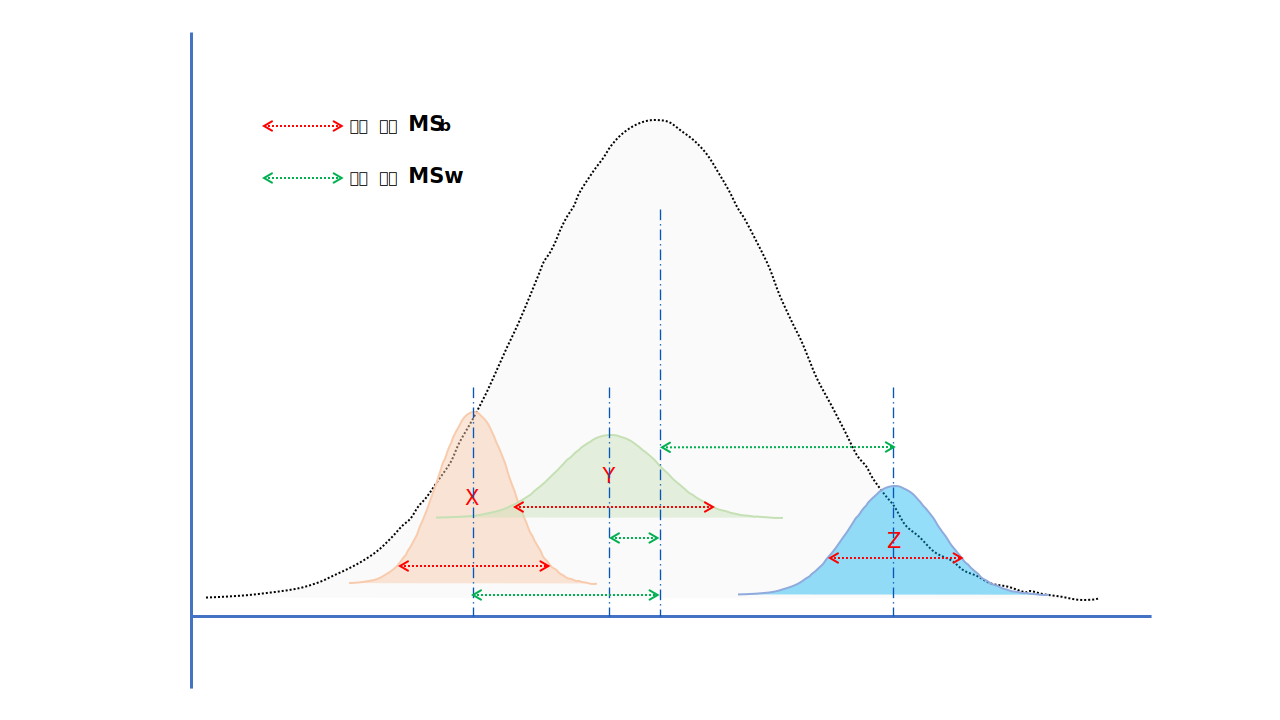
\includegraphics[width=0.7\linewidth]{image/xyzAnovaFig} 

}

\caption{三种药物来自同一总体的假设模拟及MSb,MSw示例}\label{fig:xyzanova1}
\end{figure}

根据F检验的原理,F值是组间均方\(MS_b\)和组内均方\(MS_w\)得比值,由此大概有三种情况:

\textbf{A. \(MS_b≈MS_w\),F≈1}

这个时候MSB和MSE比较近似,可能是每组的平均值很集中,且每组方差很小;或者每组的方差较大,平均值也都离的不太远。
总之,我们无法很好的剥离出某一组的分布。所以,我们同样无法拒绝\(H_0:μ_0=μ_1=μ_2=μ_3\)。

\begin{figure}

{\centering 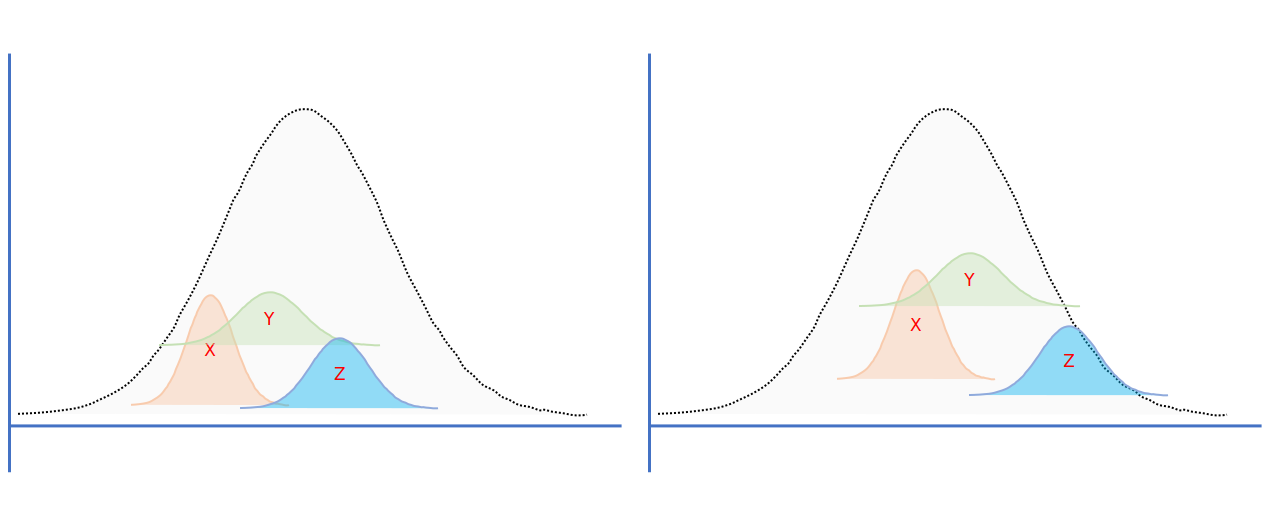
\includegraphics[width=0.7\linewidth]{image/MSbeqMSw} 

}

\caption{三种药物来自同一总体的假设模拟,MSb≈MSw示例}\label{fig:xyzanova2}
\end{figure}

\textbf{B. \(MS_b>>MS_w\),F\textgreater1}

这个情况说明,至少有一个分布相对其他分布较远,且每个分布都非常集中,即每个分组的分布方差差别较小。所以,我们不能得出三个分布都有相同的均值,
于是拒绝\(H_0:μ_0=μ_1=μ_2=μ_3\)。

\begin{figure}

{\centering 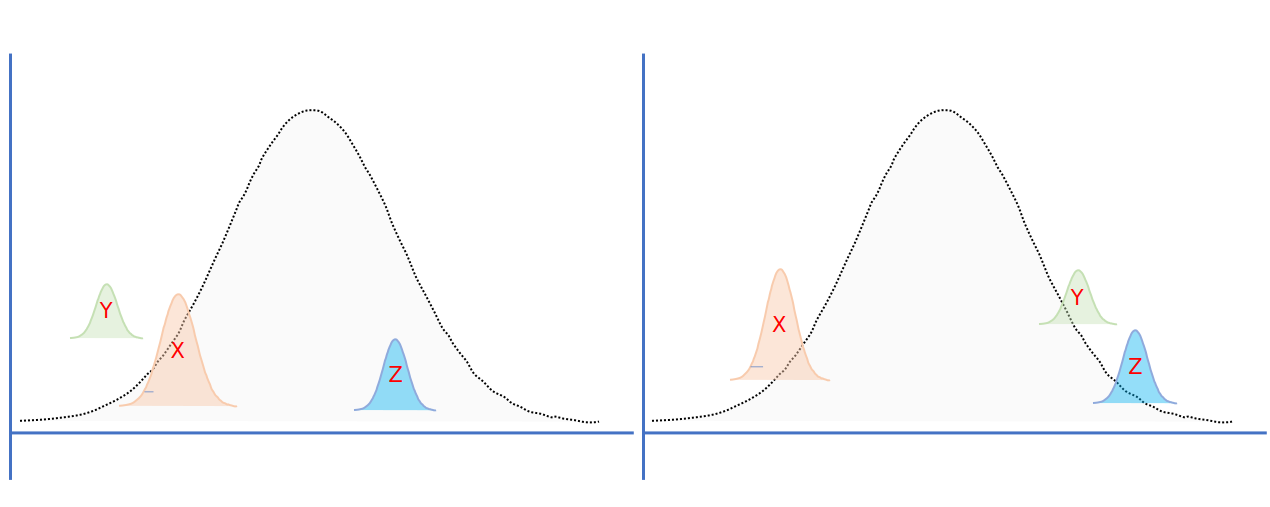
\includegraphics[width=0.7\linewidth]{image/MSbgtMSw} 

}

\caption{MSb>>MSw示例}\label{fig:xyzanova3}
\end{figure}

\textbf{C. \(MS_b<<MS_w\),F\textless1}

这个情况有两种可能,当然也可以是这两种可能的混合。一是每组的平均值都相对集中,二是每组的方差很大,导致我们无法把每组分开。所以我们无法拒绝\(H_0:μ_0=μ_1=μ_2=μ_3\)。
两个极端的例子:

\begin{figure}

{\centering 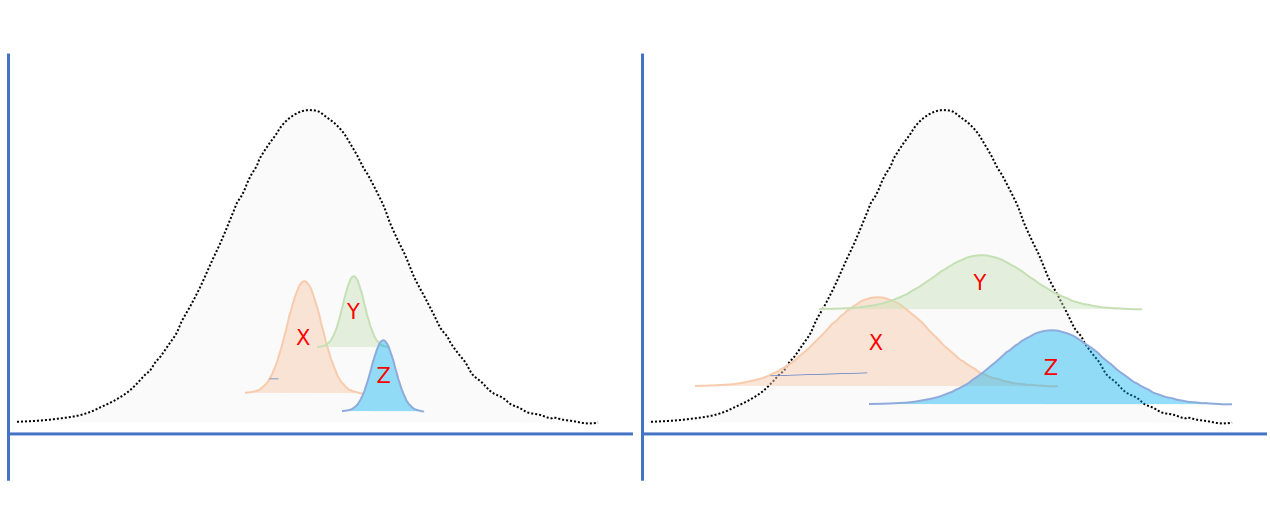
\includegraphics[width=0.7\linewidth]{image/MSbltMSw} 

}

\caption{MSb<<MSw示例}\label{fig:xyzanova4}
\end{figure}

\hypertarget{fux68c0ux9a8cux7684ux524dux63d0ux548cux5e94ux7528}{%
\paragraph{\texorpdfstring{\emph{F}检验的前提和应用}{F检验的前提和应用}}\label{fux68c0ux9a8cux7684ux524dux63d0ux548cux5e94ux7528}}

\hypertarget{ux524dux63d0}{%
\subparagraph{前提}\label{ux524dux63d0}}

F-检验是建立在一些假设基础上的,如果你的实验不能满足F-检验的假设,那你需要考虑别的分析方法或者改变实验设计。F-检验有主要有以下3个假设:

\begin{enumerate}
\def\labelenumi{\arabic{enumi}.}
\tightlist
\item
  方差的齐性,可以理解为每组样本背后的总体(也叫族群)都有相同的方差
\item
  族群遵循正态分布
\item
  每一次抽样都是独立的,比如每个病人只能提供一个数据。对于一些一个样本需要提供多个数据的情况,有其他相应的F检验方法。
\end{enumerate}

\hypertarget{ux5e94ux7528}{%
\subparagraph{应用}\label{ux5e94ux7528}}

F检验的主要有如下几种:

\begin{enumerate}
\def\labelenumi{\arabic{enumi}.}
\tightlist
\item
  \protect\hyperlink{ux4e24ux6837ux672cux65b9ux5deeux9f50ux6027ux68c0ux9a8c}{方差齐性检验(F-test of equality of variances)}
\item
  \protect\hyperlink{ux65b9ux5deeux5206ux6790}{方差分析(Analysis of Variance, ANOVA)}
\item
  线性回归方程整体的显著性检验
\end{enumerate}

\hypertarget{ux5355ux56e0ux5b50ux65b9ux5deeux5206ux6790}{%
\subsubsection{单因子方差分析}\label{ux5355ux56e0ux5b50ux65b9ux5deeux5206ux6790}}

完全随机设计(Completely random design)是采用完全随机化的分组方法,将全部实验对象分配到g个组(水平组),各组按照设计因素(单因子方差分析,One-way ANOVA)
分别接受不同水平的处理,实验结束后比较各组均数之间的差别有无统计学意义,推论因素的效应。

注意的是,当方差不齐的是否,可以使用oneway.test()函数进行F检验,设置var.equal为FALSE,
此时即为Welch检验。

使用《医学统计学》中的 案例4-2 的数据在R中进行完全随机设计资料的方差分析测试。

\begin{Shaded}
\begin{Highlighting}[]
\CommentTok{##案例4-2 }
\KeywordTok{library}\NormalTok{(}\StringTok{"memisc"}\NormalTok{)}
\CommentTok{#读取数据}
\NormalTok{rdl_sav<-}\KeywordTok{spss.system.file}\NormalTok{(}\StringTok{"ExampleData/SavData4MedSta/Exam04-02.sav"}\NormalTok{)}
\NormalTok{rdl_df<-}\KeywordTok{as.data.frame}\NormalTok{(}\KeywordTok{as.data.set}\NormalTok{(rdl_sav))}
\CommentTok{##简洁地显示任意R对象的结构}
\KeywordTok{str}\NormalTok{(rdl_df)}
\CommentTok{## 'data.frame':    120 obs. of  2 variables:}
\CommentTok{##  $ GROUP: num  1 1 1 1 1 1 1 1 1 1 ...}
\CommentTok{##  $ LDL_C: num  3.53 4.59 4.34 2.66 3.59 3.13 3.3 4.04 3.53 3.56 ...}

\CommentTok{##对不规则数组应用指定的函数,快速计算每组的均值,方差,和样本大小}
\KeywordTok{tapply}\NormalTok{(rdl_df}\OperatorTok{$}\NormalTok{LDL_C, rdl_df}\OperatorTok{$}\NormalTok{GROUP, }\DataTypeTok{FUN =}\NormalTok{ mean)}
\CommentTok{##        1        2        3        4 }
\CommentTok{## 3.430333 2.715333 2.698000 1.966333 }

\KeywordTok{tapply}\NormalTok{(rdl_df}\OperatorTok{$}\NormalTok{LDL_C, rdl_df}\OperatorTok{$}\NormalTok{GROUP, }\DataTypeTok{FUN =}\NormalTok{ var)}
\CommentTok{##         1         2         3         4 }
\CommentTok{## 0.5114033 0.4072464 0.2471752 0.5571757 }

\KeywordTok{tapply}\NormalTok{(rdl_df}\OperatorTok{$}\NormalTok{LDL_C, rdl_df}\OperatorTok{$}\NormalTok{GROUP, length)}
\CommentTok{##  1  2  3  4 }
\CommentTok{## 30 30 30 30 }

\CommentTok{#boxplot(rdl_df$LDL_C ~ rdl_df$GROUP,col=c(2:5))}

\CommentTok{## 使用oneway.test()函数进行F检验,注意var.equal 默认是 FALSE,也就是说方差可以不相等(此时即为Welch检验),但是提供的信息相对较少。}
\KeywordTok{oneway.test}\NormalTok{(rdl_df}\OperatorTok{$}\NormalTok{LDL_C }\OperatorTok{~}\StringTok{ }\NormalTok{rdl_df}\OperatorTok{$}\NormalTok{GROUP,}\DataTypeTok{var.equal=}\NormalTok{T)}
\CommentTok{##  One-way analysis of means}
\CommentTok{## }
\CommentTok{## data:  rdl_df$LDL_C and rdl_df$GROUP}
\CommentTok{## F = 24.884, num df = 3, denom df = 116, p-value = 1.674e-12}
\KeywordTok{oneway.test}\NormalTok{(rdl_df}\OperatorTok{$}\NormalTok{LDL_C }\OperatorTok{~}\StringTok{ }\NormalTok{rdl_df}\OperatorTok{$}\NormalTok{GROUP,}\DataTypeTok{var.equal=}\NormalTok{F)}
\CommentTok{##  One-way analysis of means (not assuming equal variances)}
\CommentTok{## }
\CommentTok{## data:  rdl_df$LDL_C and rdl_df$GROUP}
\CommentTok{## F = 19.665, num df = 3.000, denom df = 63.592, p-value =}
\CommentTok{## 3.924e-09}

\CommentTok{#使用aov()函数进行F检验,可以获取完整地参数信息,这里要注意aov()里面提供的group信息}
\CommentTok{#最好不要是数值形式的分组,否则结果容易当作线性回归处理,导致与预期不一致,可以用}
\CommentTok{#as.character()将数字转换为字串形式的再使用}
\NormalTok{aov.out =}\StringTok{ }\KeywordTok{aov}\NormalTok{(rdl_df}\OperatorTok{$}\NormalTok{LDL_C }\OperatorTok{~}\StringTok{ }\KeywordTok{as.character}\NormalTok{(rdl_df}\OperatorTok{$}\NormalTok{GROUP))}
\CommentTok{##                             Df Sum Sq Mean Sq F value   Pr(>F)    }
\CommentTok{## as.character(rdl_df$GROUP)   3  32.16  10.719   24.88 1.67e-12 ***}
\CommentTok{## Residuals                  116  49.97   0.431                     }
\CommentTok{## ---}
\CommentTok{## Signif. codes:  0 ‘***’ 0.001 ‘**’ 0.01 ‘*’ 0.05 ‘.’ 0.1 ‘ ’ 1}
\CommentTok{## > aov.out}
\CommentTok{## Call:}
\CommentTok{##    aov(formula = rdl_df$LDL_C ~ as.character(rdl_df$GROUP))}
\CommentTok{## }
\CommentTok{## Terms:}
\CommentTok{##                 as.character(rdl_df$GROUP) Residuals}
\CommentTok{## Sum of Squares                    32.15603  49.96702}
\CommentTok{## Deg. of Freedom                          3       116}
\CommentTok{## }
\CommentTok{## Residual standard error: 0.6563156}
\CommentTok{## Estimated effects may be unbalanced}
\KeywordTok{summary}\NormalTok{(aov.out)}
\CommentTok{##                             Df Sum Sq Mean Sq F value   Pr(>F)    }
\CommentTok{## as.character(rdl_df$GROUP)   3  32.16  10.719   24.88 1.67e-12 ***}
\CommentTok{## Residuals                  116  49.97   0.431                     }
\CommentTok{## ---}
\CommentTok{## Signif. codes:  0 ‘***’ 0.001 ‘**’ 0.01 ‘*’ 0.05 ‘.’ 0.1 ‘ ’ 1}

\CommentTok{##其他几个查看aov()对象的工具}
\KeywordTok{summary.aov}\NormalTok{(aov.out)}
\KeywordTok{summary.lm}\NormalTok{(aov.out)}
\KeywordTok{TukeyHSD}\NormalTok{(aov.out)}

\KeywordTok{boxplot}\NormalTok{(rdl_df}\OperatorTok{$}\NormalTok{LDL_C }\OperatorTok{~}\StringTok{ }\NormalTok{rdl_df}\OperatorTok{$}\NormalTok{GROUP,}\DataTypeTok{col=}\KeywordTok{c}\NormalTok{(}\DecValTok{2}\OperatorTok{:}\DecValTok{5}\NormalTok{),}\DataTypeTok{ylab=}\StringTok{"rdl value"}\NormalTok{,}\DataTypeTok{xlab=}\StringTok{"Group info"}\NormalTok{)}
\end{Highlighting}
\end{Shaded}

\begin{figure}

{\centering 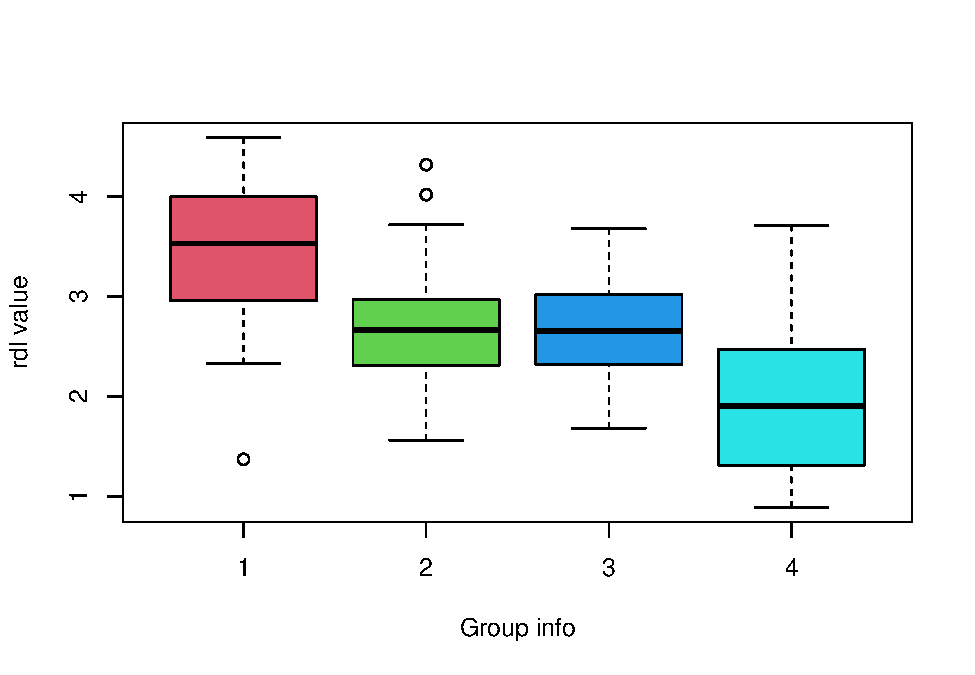
\includegraphics[width=0.6\linewidth]{figs/Cmdftest} 

}

\caption{案例 04-02 120例数据的箱线图预览}\label{fig:Cmdftest}
\end{figure}

\begin{table}

\caption{\label{tab:tab2}案例04-02 F检验结果}
\centering
\begin{tabular}[t]{lcc}
\toprule
  & 组间 & 组内\\
\midrule
自由度 & 3.000 & 116.0000\\
SS & 32.156 & 49.9670\\
MS & 10.719 & 0.4308\\
F值 & 24.884 & \\
P值 & 0.000 & \\
\bottomrule
\end{tabular}
\end{table}

根据计算结果,F值=24.884\textgreater{}\(F_{(0.01,(3,116))}\),P值\textless0.01\textless0.05,按照α=0.05的检验水准,拒绝\(H_0\),接受
\(H_1\),认为4个处理组的总体均数不全相等。

在方差分析的基本操作结束后,我们还可以利用线性回归的工具对方差分析的结果拟合情况进行评估,详细可参考\protect\hyperlink{ux65b9ux5deeux5206ux6790ux7684ux8bcaux65adux56fe}{方差分析的诊断图}。

\hypertarget{ux53ccux56e0ux5b50ux65b9ux5deeux5206ux6790}{%
\subsubsection{双因子方差分析}\label{ux53ccux56e0ux5b50ux65b9ux5deeux5206ux6790}}

随机区组设计(Randomized block design)又称为配伍组设计,是配对设计的扩展。具体做法是:先按影响实验结果的
非处理因素(如性别、体重、年龄、职业、病情、病程等)将实验对象配成区组(Block),再分 别将各区组内的实验对象
随机分配到各处理组或对照组。与完全随机设计相比,随机区组设计的特点是 随机分配的次数要重复多次,每次随机分
配都对同一个区组内的实验对象进行,且各个处理组的实验对象数量相同,区组内均衡。在进行统计分析时,将区组
变异离均差平方和从完全随机设计的组內离均差平和 中分离出来,从而减小组内离均差平方和(误差平方和),提高统
计检验效率。若将区组作为另一处理因素 的不同水平,随机区组设计等同于无重复观察的两因素设计(双因子方差分析,Two-way ANOVA)。

随机区组设计资料在进行统计分析时,需根据数据的分布特征选择方法,对于正态分布且方差齐同的资料,采用双向分类的
方差分析(Two-way classification ANOVA)或配对\protect\hyperlink{ux2atux2aux5cux2520ux68c0ux9a8cux7684ux5206ux7c7bux53caux5e94ux7528}{\emph{t}检验(g=2)};当不满足方差分析或\emph{t}检验条件时,可进行变量变换后采
用双向分类的方差分析或采用\protect\hyperlink{Friedmanux5cux2520Mux68c0ux9a8c}{Friedman M检验}。

双向ANOVA分析是单向ANOVA的扩展,分析两个因素,我们称之为A和B,假如A有i(1\textsubscript{g)个水平(或叫区组),B有j(1}n)个水平(处理因素的水平),
且每个分组的样本数目要一致,则共有\(N=ng\)样本个体,记总均数为\(\bar{X}\),各处理组均数分别是\(\bar{X_i}\),
各区组均数为\(\bar{X_{i}}\),双向ANOVA的实验数据有四个不同的变异:

\textbf{1. 总变异},它反应所有观测值之间的变异,总离均差平方和:\(SS_{total}\)

\textbf{2. 处理组间变异},它反应处理因素的不同水平作用和随机误差产生的变异:\(SS_{treat}\)

\textbf{3. 区组间变异},它反应不同区组作用和随机误差产生的变异:\(SS_{block}\)

\textbf{4. 误差变异},它是完全由随机误差产生的变异:\(SS_{error}\)

对总离均差平方和及自由度的分解关系为:
\[\begin{aligned}
SS_{total} & = SS_{treat}+SS_{block}+SS_{error} \\
v_{total} & = v_{treat}+v_{block}+v_{error}
\end{aligned}\]

其中\(v_{total}=N-1\),\(v_{treat}=g-1\),\(v_{block}=n-1\),
\(v_{error}=v_{treat}v_{block}=(n-1)(g-1)\)。

误差变异的均方差即为;\(MS_{error}=SS_{error}/v_{error}\),

处理组间变异的均方差即为:\(MS_{treat}=SS_{treat}/v_{treat}\),

区组间变异均方差即为:\(MS_{block}=SS_{block}/v_{block}\),

处理组间变异的F值公式:\(F_{treat}=\frac{MS_{treat}}{MS_{error}}\)

区组间变异的F值公式:\(F_{block}=\frac{MS_{block}}{MS_{error}}\)

双向ANOVA能够同时检验3个零假设:

\begin{enumerate}
\def\labelenumi{\arabic{enumi}.}
\item
  单独考虑A因素,总体均值间没有差别,这相当于对A因子进行单向ANOVA
\item
  单独考虑B因素,总体均值间没有差别,这相当于对B因子进行单向ANOVA
\item
  A和B两个因素,没有相互作用,相当于使用二联表进行独立性分析
\end{enumerate}

使用《医学统计学》中的 案例4-4 的数据在R中进行双因子方差分析的测试。

\begin{Shaded}
\begin{Highlighting}[]
\KeywordTok{library}\NormalTok{(}\StringTok{"memisc"}\NormalTok{)}
\NormalTok{sarc_sav<-}\KeywordTok{spss.system.file}\NormalTok{(}\StringTok{"ExampleData/SavData4MedSta/Exam04-04.sav"}\NormalTok{)}
\NormalTok{sarc_df<-}\KeywordTok{as.data.frame}\NormalTok{(}\KeywordTok{as.data.set}\NormalTok{(sarc_sav))}
\KeywordTok{str}\NormalTok{(sarc_df)}
\CommentTok{## 'data.frame':    15 obs. of  3 variables:}
\CommentTok{##  $ GROUP : num  1 2 3 4 5 1 2 3 4 5 ...}
\CommentTok{##  $ TREAT : num  1 1 1 1 1 2 2 2 2 2 ...}
\CommentTok{##  $ WEIGHT: num  0.82 0.73 0.43 0.41 0.68 0.65 0.54 0.34 0.21 0.43 ...}

\NormalTok{sarc_aov.out<-}\KeywordTok{aov}\NormalTok{(sarc_df}\OperatorTok{$}\NormalTok{WEIGHT }\OperatorTok{~}\StringTok{ }\KeywordTok{factor}\NormalTok{(}\KeywordTok{as.character}\NormalTok{(sarc_df}\OperatorTok{$}\NormalTok{TREAT))}\OperatorTok{+}\KeywordTok{factor}\NormalTok{(}\KeywordTok{as.character}\NormalTok{(sarc_df}\OperatorTok{$}\NormalTok{GROUP)))}
\CommentTok{## Call:}
\CommentTok{##    aov(formula = sarc_df$WEIGHT ~ factor(as.character(sarc_df$TREAT)) + }
\CommentTok{##     factor(as.character(sarc_df$GROUP)))}
\CommentTok{## }
\CommentTok{## Terms:}
\CommentTok{##                 factor(as.character(sarc_df$TREAT)) factor(as.character(sarc_df$GROUP)) Residuals}
\CommentTok{## Sum of Squares                              0.22800                             0.22836   0.07640}
\CommentTok{## Deg. of Freedom                                   2                                   4         8}
\CommentTok{## }
\CommentTok{## Residual standard error: 0.0977241}
\CommentTok{## Estimated effects may be unbalanced}
\KeywordTok{summary}\NormalTok{(sarc_aov.out)}
\CommentTok{##                                     Df Sum Sq Mean Sq F value  Pr(>F)   }
\CommentTok{## factor(as.character(sarc_df$TREAT))  2 0.2280 0.11400  11.937 0.00397 **}
\CommentTok{## factor(as.character(sarc_df$GROUP))  4 0.2284 0.05709   5.978 0.01579 * }
\CommentTok{## Residuals                            8 0.0764 0.00955                   }
\CommentTok{## ---}
\CommentTok{## Signif. codes:  0 ‘***’ 0.001 ‘**’ 0.01 ‘*’ 0.05 ‘.’ 0.1 ‘ ’ 1}

\CommentTok{##其他几个查看aov()对象的工具}
\KeywordTok{summary.aov}\NormalTok{(sarc_aov.out)}
\KeywordTok{summary.lm}\NormalTok{(sarc_aov.out)}
\KeywordTok{TukeyHSD}\NormalTok{(sarc_aov.out)}
\end{Highlighting}
\end{Shaded}

\begin{table}

\caption{\label{tab:tab3}案例04-04 双因子f检验结果}
\centering
\begin{tabular}[t]{lccccc}
\toprule
  & 自由度 & SS & MS & F值 & P值\\
\midrule
处理间 & 2 & 0.2280 & 0.1140 & 11.937 & 0.0040\\
区组间 & 4 & 0.2284 & 0.0571 & 5.978 & 0.0158\\
误差 & 8 & 0.0764 & 0.0096 &  & \\
\bottomrule
\end{tabular}
\end{table}

根据计算结果,对于处理组间F值为11.937,对应P值是0.004\textless0.01\textless α=0.05,因此拒绝处理组间\(H_0: μ_1=μ_2=μ_3\)的原假设,接受\(H_1\),即认为
药物的肿瘤生长有统计学意义。同理,区组间的F值为5.978,对应的P值是0.0158\textless α=0.05,因此拒绝区组间的\(H_0: μ_1=μ_2=μ_3\)的原假设,
接受\(H_1\),即体重对肿瘤生长的影响有统计学意义。

现在有一个问题,是方差分析的结果可以推断多组样本的总体之间的均值是否都相等,如果不都相等,我怎么知道是具体是怎么不相等的呢?
详细请看\protect\hyperlink{ux591aux4e2aux6837ux672cux5747ux6570ux8bb2ux7684ux591aux91cdux6bd4ux8f83}{多重比较}。

\hypertarget{ux62c9ux4e01ux65b9ux8bbeux8ba1ux8d44ux6599ux7684ux65b9ux5deeux5206ux6790}{%
\subsubsection{拉丁方设计资料的方差分析}\label{ux62c9ux4e01ux65b9ux8bbeux8ba1ux8d44ux6599ux7684ux65b9ux5deeux5206ux6790}}

完全随机设计只涉及一个处理因素;随机区组设计涉及一个处理因素、一个区组因素(或称为配伍因素);
倘若实验研究涉及一个处理因素和两个控制因素,每个因素的类别数或水平数相等,此时可采用拉丁方
设计(Latin square design)来安排实验,将两个控制因素分别安排在拉丁方设计的行和列上。拉丁方
设计是在随机区组设计的基础上发展的,它可多安排一个已知的对实验结果有影响的非处理 因素,增加
了均衡性,减少了误差,提高了效率。

拉丁方设计资料采用三向分类的方差分析(Three-way classification ANOVA),总变异可分解为处理
组变异、行区组变异、列区组变异和误差4部分,比如对于一个g*g的拉丁方实验设计,用i,j,k分别代表捏区组水平,
行区组水平和处理因素的水平,它们和对应的自由度分别是:

\textbf{1. 总变异},它反应所有观测值之间的变异,总离均差平方和:\(SS_{total}\)

\textbf{2. 处理组间变异},它反应处理因素的不同水平作用和随机误差产生的变异:\(SS_{treat}\)

\textbf{3. 列区组间变异},它反应不同列区组作用和随机误差产生的变异:\(SS_{column}\)

\textbf{4. 行区组间变异},它反应不同行区组作用和随机误差产生的变异:\(SS_{row}\)

\textbf{5. 误差变异},它是完全由随机误差产生的变异:\(SS_{error}\)

对总离均差平方和及自由度的分解关系为:
\[\begin{aligned}
SS_{total} &= SS_{treat}+SS_{column}+SS_{row}+SS_{error}\\
v_{total} &= v_{treat}+v_{column}+v_{row}+v_{error}
\end{aligned}\]

其中\(v_{total}=N-1=g^2-1\),\(v_{treat}=g-1=\)v\_\{column\}=v\_\{column\}=g-1\$,
\(v_{error}=(g-2)(g-1)\)。

误差变异的均方差即为;\(MS_{error}=SS_{error}/v_{error}\),

处理组间变异的均方差即为:\(MS_{treat}=SS_{treat}/v_{treat}\),

列区组间变异均方差即为:\(MS_{column}=SS_{column}/v_{column}\),

行区组间变异均方差即为:\(MS_{row}=SS_{row}/v_{row}\),

处理组间变异的F值公式:\(F_{treat}=\frac{MS_{treat}}{MS_{error}}\)

列区组间变异的F值公式:\(F_{column}=\frac{MS_{column}}{MS_{error}}\)

行区组间变异的F值公式:\(F_{row}=\frac{MS_{row}}{MS_{error}}\)

拉丁方设计资料采用三向分类的ANOVA,由于比较复杂,在分析之前应该理清楚处理组,列区组。行区组的
对应的因素,并理清它们各自的原假设与备择假设,总的来说能够同时检验3个零假设:

\begin{enumerate}
\def\labelenumi{\arabic{enumi}.}
\item
  处理组之间的总体均数都相等
\item
  列区组之间的总体均数都相等
\item
  行区组之间的总体均数都相等
\end{enumerate}

使用《医学统计学》中的 案例4-5 的数据在R中进行拉丁方实验设计资料的方差分析测试。

\begin{Shaded}
\begin{Highlighting}[]
\KeywordTok{library}\NormalTok{(}\StringTok{"memisc"}\NormalTok{)}
\NormalTok{hsv_sav<-}\KeywordTok{spss.system.file}\NormalTok{(}\StringTok{"ExampleData/SavData4MedSta/Exam04-05.sav"}\NormalTok{)}
\NormalTok{hsv_df<-}\KeywordTok{as.data.frame}\NormalTok{(}\KeywordTok{as.data.set}\NormalTok{(hsv_sav))}
\KeywordTok{str}\NormalTok{(hsv_df)}
\CommentTok{## 'data.frame':    36 obs. of  4 variables:}
\CommentTok{##  $ 行区组  : num  1 1 1 1 1 1 2 2 2 2 ...}
\CommentTok{##   ..- attr(*, "label")= chr "<RMC1`:E"}
\CommentTok{##  $ 列区组  : num  1 2 3 4 5 6 1 2 3 4 ...}
\CommentTok{##  $ 处理组  : num  3 2 5 4 1 6 2 1 4 3 ...}
\CommentTok{##   ..- attr(*, "label")= chr "2;M,R)No"}
\CommentTok{##  $ 实验结果: num  87 75 81 75 84 66 73 81 87 85 ...}
\CommentTok{##修改一下列名称}
\KeywordTok{colnames}\NormalTok{(hsv_df)<-}\KeywordTok{c}\NormalTok{(}\StringTok{"rg"}\NormalTok{,}\StringTok{"lg"}\NormalTok{,}\StringTok{"tg"}\NormalTok{,}\StringTok{"test_val"}\NormalTok{)}
\NormalTok{hsv_aov.out <-}\KeywordTok{aov}\NormalTok{(hsv_df}\OperatorTok{$}\NormalTok{test_val }\OperatorTok{~}\StringTok{ }\KeywordTok{factor}\NormalTok{(}\KeywordTok{as.character}\NormalTok{(hsv_df}\OperatorTok{$}\NormalTok{tg))}\OperatorTok{+}\KeywordTok{factor}\NormalTok{(}\KeywordTok{as.character}\NormalTok{(hsv_df}\OperatorTok{$}\NormalTok{rg))}\OperatorTok{+}\KeywordTok{factor}\NormalTok{(}\KeywordTok{as.character}\NormalTok{(hsv_df}\OperatorTok{$}\NormalTok{lg)))}
\KeywordTok{summary}\NormalTok{(hsv_aov.out)}
\CommentTok{##                                 Df Sum Sq Mean Sq F value Pr(>F)  }
\CommentTok{## factor(as.character(hsv_df$tg))  5    667   133.4    3.79  0.014 *}
\CommentTok{## factor(as.character(hsv_df$rg))  5    250    50.1    1.42  0.258  }
\CommentTok{## factor(as.character(hsv_df$lg))  5     65    13.1    0.37  0.862  }
\CommentTok{## Residuals                       20    703    35.2                 }
\CommentTok{## ---}
\CommentTok{## Signif. codes:  0 ‘***’ 0.001 ‘**’ 0.01 ‘*’ 0.05 ‘.’ 0.1 ‘ ’ 1}
\KeywordTok{summary.aov}\NormalTok{(hsv_aov.out)}
\KeywordTok{summary.lm}\NormalTok{(hsv_aov.out)}
\KeywordTok{TukeyHSD}\NormalTok{(hsv_aov.out)}
\end{Highlighting}
\end{Shaded}

\begin{table}

\caption{\label{tab:tab4}案例04-05 拉丁方设计资料采用三向分类的f检验结果}
\centering
\begin{tabular}[t]{lccccc}
\toprule
  & 自由度 & SS & MS & F值 & P值\\
\midrule
处理间 & 5 & 667.139 & 133.428 & 3.7940 & 0.0140\\
家兔间 & 5 & 250.472 & 50.094 & 1.4244 & 0.2584\\
部位间 & 5 & 65.337 & 13.067 & 0.3716 & 0.8621\\
误差 & 20 & 703.358 & 35.168 &  & \\
\bottomrule
\end{tabular}
\end{table}

根据计算结果,对于处理组间F值为3.79402,对应P值是0.014\textless α=0.05,因此拒绝处理组间\(H_0\)的原假设,接受\(H_1\),即认为
6种药物的对疱疹大小的生长影响有统计学意义。同理,家兔间的F值为1.42444,对应的P值是0.258401\textgreater α=0.05,因此暂时不能拒绝家兔间的\(H_0\)的原假设,
即还不能认为疱疹的大小的总体均数不全相等。对于部位间的F值为0.37157,对应的P值是0.862102\textgreater α=0.05,因此暂时不能拒绝部位间的\(H_0\)的原假设,
即还不能认为6个部位的疱疹大小的总体均数不全相等。

\hypertarget{ux4e24ux9636ux6bb5ux4ea4ux53c9ux8bbeux8ba1ux8d44ux6599ux7684ux65b9ux5deeux5206ux6790}{%
\subsubsection{两阶段交叉设计资料的方差分析}\label{ux4e24ux9636ux6bb5ux4ea4ux53c9ux8bbeux8ba1ux8d44ux6599ux7684ux65b9ux5deeux5206ux6790}}

在医学研究中,欲将A、B两种处理先后施加于同一批实验对象,随机地使半数实验对象先接受A后 接受B,而另一半实验对象
则正好相反,即先接受B再接受A。由于两种处理在全部实验过程中交叉进 行,这种设计称为交叉设计(Crossover design)。
在交叉设计中,A、B两种处理先后以同等的机会出现在两 个实验阶段中,故又称为两阶段交叉设计。当然也可以有多个实验
阶段,但本节仅介绍两阶段的交叉设 计。虽然交叉实验的处理是单因素,但影响实验结果的因素还有非人为控制的实验对
象的个体差异和实 验阶段这两个因素。因此,该设计不仅平衡了处理顺序的影响,而且能把处理方法间的差别、时间先后之
间的差别和实验对象之间的差别分开来分析。但是该设计有一个较为严格的限制条件:前一个实验阶段的处理效应不能持续
作用到下一个实验阶段。为此,有必要在两个阶段之间设一个洗脱(Wash-out)阶段, 以消除残留效应(Carry-over effect)
的影响。在医学研究中交叉设计多用于止痛、镇静、降压等药物或治疗方法间疗效的比较。

使用《医学统计学》中的 案例4-5 的数据在R中进行两阶段交叉设计资料的方差分析测试。

\begin{Shaded}
\begin{Highlighting}[]
\KeywordTok{library}\NormalTok{(}\StringTok{"memisc"}\NormalTok{)}
\NormalTok{gmp_sav<-}\KeywordTok{spss.system.file}\NormalTok{(}\StringTok{"ExampleData/SavData4MedSta/Exam04-06.sav"}\NormalTok{)}
\NormalTok{gmp_df<-}\KeywordTok{as.data.frame}\NormalTok{(}\KeywordTok{as.data.set}\NormalTok{(gmp_sav))}
\KeywordTok{str}\NormalTok{(gmp_df)}
\CommentTok{## 'data.frame':    20 obs. of  4 variables:}
\CommentTok{##  $ PERSON: num  1 2 3 4 5 6 7 8 9 10 ...}
\CommentTok{##   ..- attr(*, "label")= chr "J\textbackslash{}\textbackslash{}JTU_1`:E"}
\CommentTok{##  $ TREAT : num  1 2 1 1 2 2 1 2 1 2 ...}
\CommentTok{##   ..- attr(*, "label")= chr "IAK8R:"}
\CommentTok{##  $ PHASE : num  1 1 1 1 1 1 1 1 1 1 ...}
\CommentTok{##   ..- attr(*, "label")= chr "=W6N"}
\CommentTok{##  $ X     : num  760 860 568 780 960 940 635 440 528 800 ...}
\CommentTok{##   ..- attr(*, "label")= chr "Q*=,3H-cGMP"}
\NormalTok{gmp_aov.out <-}\KeywordTok{aov}\NormalTok{(gmp_df}\OperatorTok{$}\NormalTok{X }\OperatorTok{~}\StringTok{ }\KeywordTok{factor}\NormalTok{(}\KeywordTok{as.character}\NormalTok{(gmp_df}\OperatorTok{$}\NormalTok{PERSON))}\OperatorTok{+}\KeywordTok{factor}\NormalTok{(}\KeywordTok{as.character}\NormalTok{(gmp_df}\OperatorTok{$}\NormalTok{TREAT))}\OperatorTok{+}\KeywordTok{factor}\NormalTok{(}\KeywordTok{as.character}\NormalTok{(gmp_df}\OperatorTok{$}\NormalTok{PHASE)))}
\CommentTok{## summary(gmp_aov.out)}
\CommentTok{##                                     Df Sum Sq Mean Sq F value  Pr(>F)    }
\CommentTok{## factor(as.character(gmp_df$PERSON))  9 551111   61235 1240.19 1.3e-11 ***}
\CommentTok{## factor(as.character(gmp_df$TREAT))   1    198     198    4.02   0.080 .  }
\CommentTok{## factor(as.character(gmp_df$PHASE))   1    490     490    9.93   0.014 *  }
\CommentTok{## Residuals                            8    395      49                    }
\CommentTok{## ---}
\CommentTok{## Signif. codes:  0 ‘***’ 0.001 ‘**’ 0.01 ‘*’ 0.05 ‘.’ 0.1 ‘ ’ 1}
\KeywordTok{summary.aov}\NormalTok{(gmp_aov.out)}
\KeywordTok{summary.lm}\NormalTok{(gmp_aov.out)}
\KeywordTok{TukeyHSD}\NormalTok{(gmp_aov.out)}
\end{Highlighting}
\end{Shaded}

\begin{table}

\caption{\label{tab:tab5}案例04-05 两阶段交叉设计资料的f检验结果}
\centering
\begin{tabular}[t]{lccccc}
\toprule
  & 自由度 & SS & MS & F值 & P值\\
\midrule
处理间 & 1 & 198.45 & 198.450 & 4.0192 & 0.0799\\
阶段间 & 1 & 490.05 & 490.050 & 9.9251 & 0.0136\\
受试者间 & 9 & 551111.45 & 61234.606 & 1240.1945 & 0.0000\\
误差 & 8 & 395.00 & 49.375 &  & \\
\bottomrule
\end{tabular}
\end{table}

根据计算结果,还不能认为A和B两种闪烁液的测定结果有差别;可认为测定阶段对测定结果有影响:可认为各受试者的H-cGMP
值不同。交叉试验主要关心处理间的差别,I、II阶段和受试者间通常是已知的控制因素。

\hypertarget{ux65b9ux5deeux5206ux6790ux7684ux8bcaux65adux56fe}{%
\subsection{方差分析的诊断图}\label{ux65b9ux5deeux5206ux6790ux7684ux8bcaux65adux56fe}}

当我们进行方差分析后,统计软件会输出一堆数字,我们在推断结果是显著的(或不显著的),
你可能认为你已经完成了分析,但我们通常还应该检查方差分析是否适合数据。可以怎么做呢?

这里要补充一点说明线性回归和方差分析的关系。从数学的观点,线性回归和方差分析是相同的:
两者将数据的总方差拆分不同的``子方差'',并用检验(F检验)来验证这些``子方差''的相等性。线性
回归和方差分析稍有区别的是,在这两种技术中因变量是连续的,但在ANOVA分析中,自变量可以是专有的分
类变量,而在回归中,可以使用分类和连续自变量。因此,方差分析可以被认为是线性回归的一个案例,其中
所有的预测因子都是分类变量。关于线性回归和方差分析,以后有时间在做更详细的比较说明吧。

所以,我们可以用检查线性回归的模型中用到一些方法来辅助查看方差分析结果。R中线性回归分析的内置诊断图
(Diagnostic Plots,除了内置的基本R函数之外,还有许多其他方法可以探索数据和诊断线性模型)它非常容易运行:
只需在运行分析之后对lm对象或者aov对象使用plot()。然后R将依次向您展示四个残差(估计值与真实值之差)相关的诊断图:

\begin{enumerate}
\def\labelenumi{\arabic{enumi}.}
\tightlist
\item
  Residuals vs Fitted
\item
  Normal Q-Q
\item
  Scale-Location
\item
  Residuals vs Leverage
\end{enumerate}

下面是用单因子方差分析结果做示例的代码和说明。

\begin{Shaded}
\begin{Highlighting}[]
\CommentTok{##用aov()的残差诊断图检验方差分析结果}
\KeywordTok{par}\NormalTok{(}\DataTypeTok{mfrow=}\KeywordTok{c}\NormalTok{(}\DecValTok{2}\NormalTok{,}\DecValTok{2}\NormalTok{))}
\KeywordTok{plot}\NormalTok{(aov.out)}
\end{Highlighting}
\end{Shaded}

\begin{figure}

{\centering 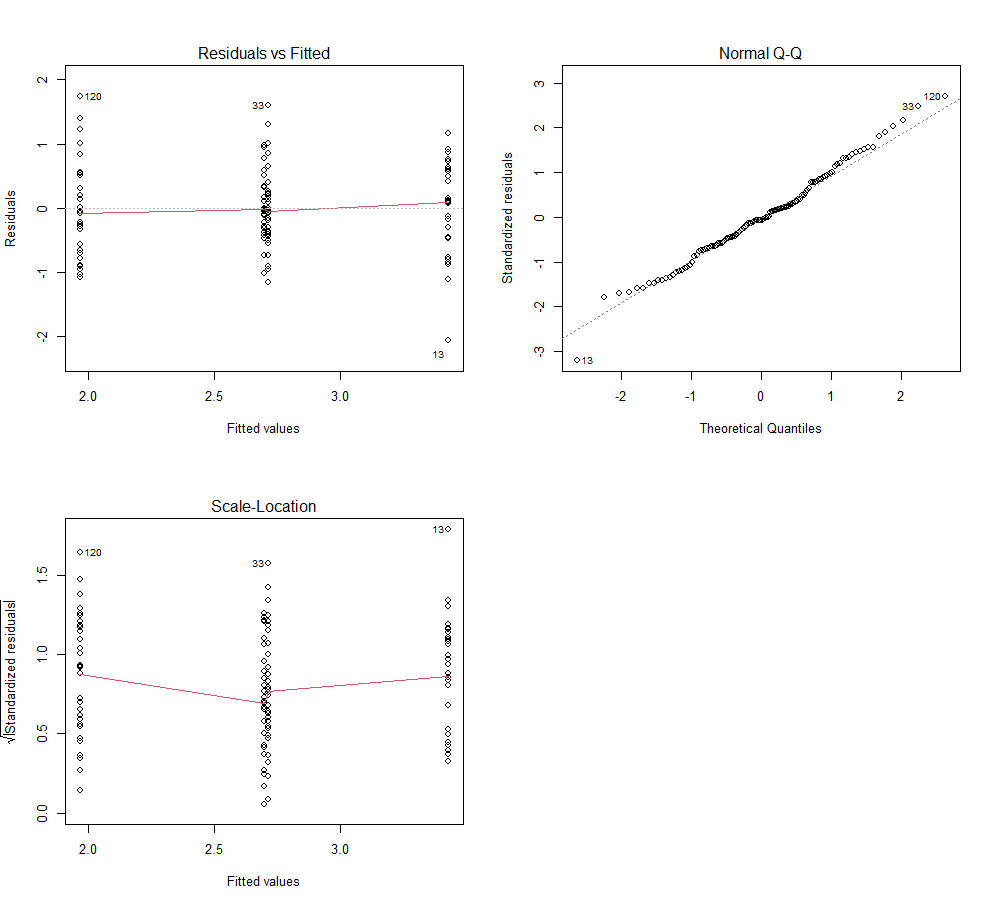
\includegraphics[width=0.6\linewidth]{image/diagnosticplots} 

}

\caption{aov()的残差诊断图}\label{fig:diagnosticplots1}
\end{figure}

\textbf{1. Residuals vs Fitted}

此图就是残差与真实值之间的关系图。在理想线性模型中有五大假设。其中之一便是残差应该是一个正态分布,与估计值无关。
在线性回归当中,如果残差还和估计值有关(即不是一次函数关系,非线性关系),那就说明模型仍然有值得去改进的地方。
对于方差分析,如果残差还和估计值有关,通常说明样本数据均值不同,或者方差不齐等问题。

\textbf{2. Normal Q-Q}

此图是验证残差的正态分布性,即残差是否沿直线良好或严重偏离? 如果残差在不是虚线上很好地对齐,则是不是正态分布,
表明样本数据可能不符合方差分析的假设前提。

\textbf{3. Scale-Location}

Spread-Location plot,测试残差是否随着拟合值的增加而增加,显示残差是否在预测变量的范围内平均分布。
这样可以检查方差齐性(Homoscedasticity,均方差)的假设。如果您看到一条具有相等(随机)分布点的(近似)水平直线,表明各组
之间方差齐性。

\textbf{4. Residuals vs Leverage}

本案例中的数据数据比较乖巧,没有特别极端的数据,因此没有画出来。
方差分析结果绘制Residuals vs Leverage图类似\ref{fig:diagnosticplots2},可以直观的告诉我们哪一组分组数据拟合的最好。

线性回归分析绘制的Residuals vs Leverage图可以帮助我们找到有影响力的案例(例如受试者)。在线性回归分析中,并非所有的离群值(Outliers)
都有影响。即使数据具有极端值,它们也可能不会对确定回归线产生影响。这意味着,如果我们在分析中包括或排除它们,
结果也不会有太大不同。在大多数情况下,它们都是遵循趋势的,它们并不重要,他们没有影响力。
另一方面,有些案例可能非常有影响力,即使它们看起来在合理的价值范围内,它们可能是与回归线相反的极端情况,
如果我们将它们排除在分析之外,结果可能会发生改变。或者说,在大多数情况下,它们并不认同这种趋势。

\begin{figure}

{\centering 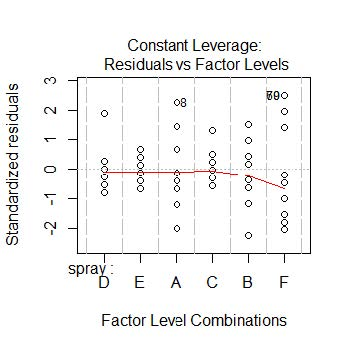
\includegraphics[width=0.6\linewidth]{image/diagnosticplots2} 

}

\caption{aov()的残差诊断图Leverage}\label{fig:diagnosticplots2}
\end{figure}

\hypertarget{ux591aux4e2aux6837ux672cux5747ux6570ux95f4ux7684ux591aux91cdux6bd4ux8f83}{%
\subsection{多个样本均数间的多重比较}\label{ux591aux4e2aux6837ux672cux5747ux6570ux95f4ux7684ux591aux91cdux6bd4ux8f83}}

当方差分析的结果为拒绝\(H_0\),接受\(H_1\)时,只说明g个总体均数不全相等。若想进一步了解哪两个总体均数不等,
须进行多个样本均数间的两两比较或称多重比较(Multiple comparison)。这种进一步阐明在ANOVA测试中起重要作
用的群体差异的方法,叫做事后测试(Post hoc tests)。如用案例4-2 的两样本均数比较的检验进行
多重比较,将会加大犯I型错误(把总体均数间本无差别判为有差别)的概。若用\emph{t}检验作6次比较,且每次比较的检验
水准选为α=0.05,则每次比较不犯I类错误的概率为(1-0.05),6次均不犯I类错误的概率为(1-0.05),这时,
总的检验水准变为1-(1-0.05)=026,比0.05大多了。因此,样本均数间的多重比较不能用两样本均数比较的检验。

事后测试分析测试非常重要,因为尽管ANOVA提供了很多信息,但它并未提供有关特定研究组之间差异的详细信息,也无法提供有关复杂比较的信息。
这些事后测试的进一步分析可能会为研究人员提供该研究的最重要发现。可供我们选择的事后测试统计方法更有10多种,
但是目前还没有一种在任何条件下都适用、效果好的方法。因此,选择与数据相匹配的测试方法,进行组间比较有关的信
息种类以及必要的分析就非常重要。方法选择不当的后果通常与第Ⅰ类错误有关,但也可能涉及未能发现组之间的重要差异。
进一步了解可以阅读:

\begin{enumerate}
\def\labelenumi{\arabic{enumi}.}
\tightlist
\item
  \href{https://www.biochemia-medica.com/en/journal/21/3/10.11613/BM.2011.029/fullArticle}{McHugh ML. 2011. Multiple comparison analysis testing in ANOVA}。
\item
  \href{https://cran.r-project.org/web/packages/agricolae/vignettes/tutorial.pdf}{agricolae tutorial (Version 1.3-3)}
\item
  \href{http://www.ievbras.ru/ecostat/Kiril/R/Biblio_N/R_Eng/Bretz2011.pdf}{Multiple Comparisons Using R}
\item
  \href{https://stat.ethz.ch/R-manual/R-devel/library/stats/html/p.adjust.html}{Adjust P-values for Multiple Comparisons}
\item
  知乎上的\href{https://zhuanlan.zhihu.com/p/44880434}{方差分析之多重比较}。
\end{enumerate}

不同多重比较(Multiple comparison)的比较与他们在R语言中的实现方法,可以参考下面的图表,具体的函数使用和参数设置请查看相应的帮助文档。

\begin{figure}

{\centering 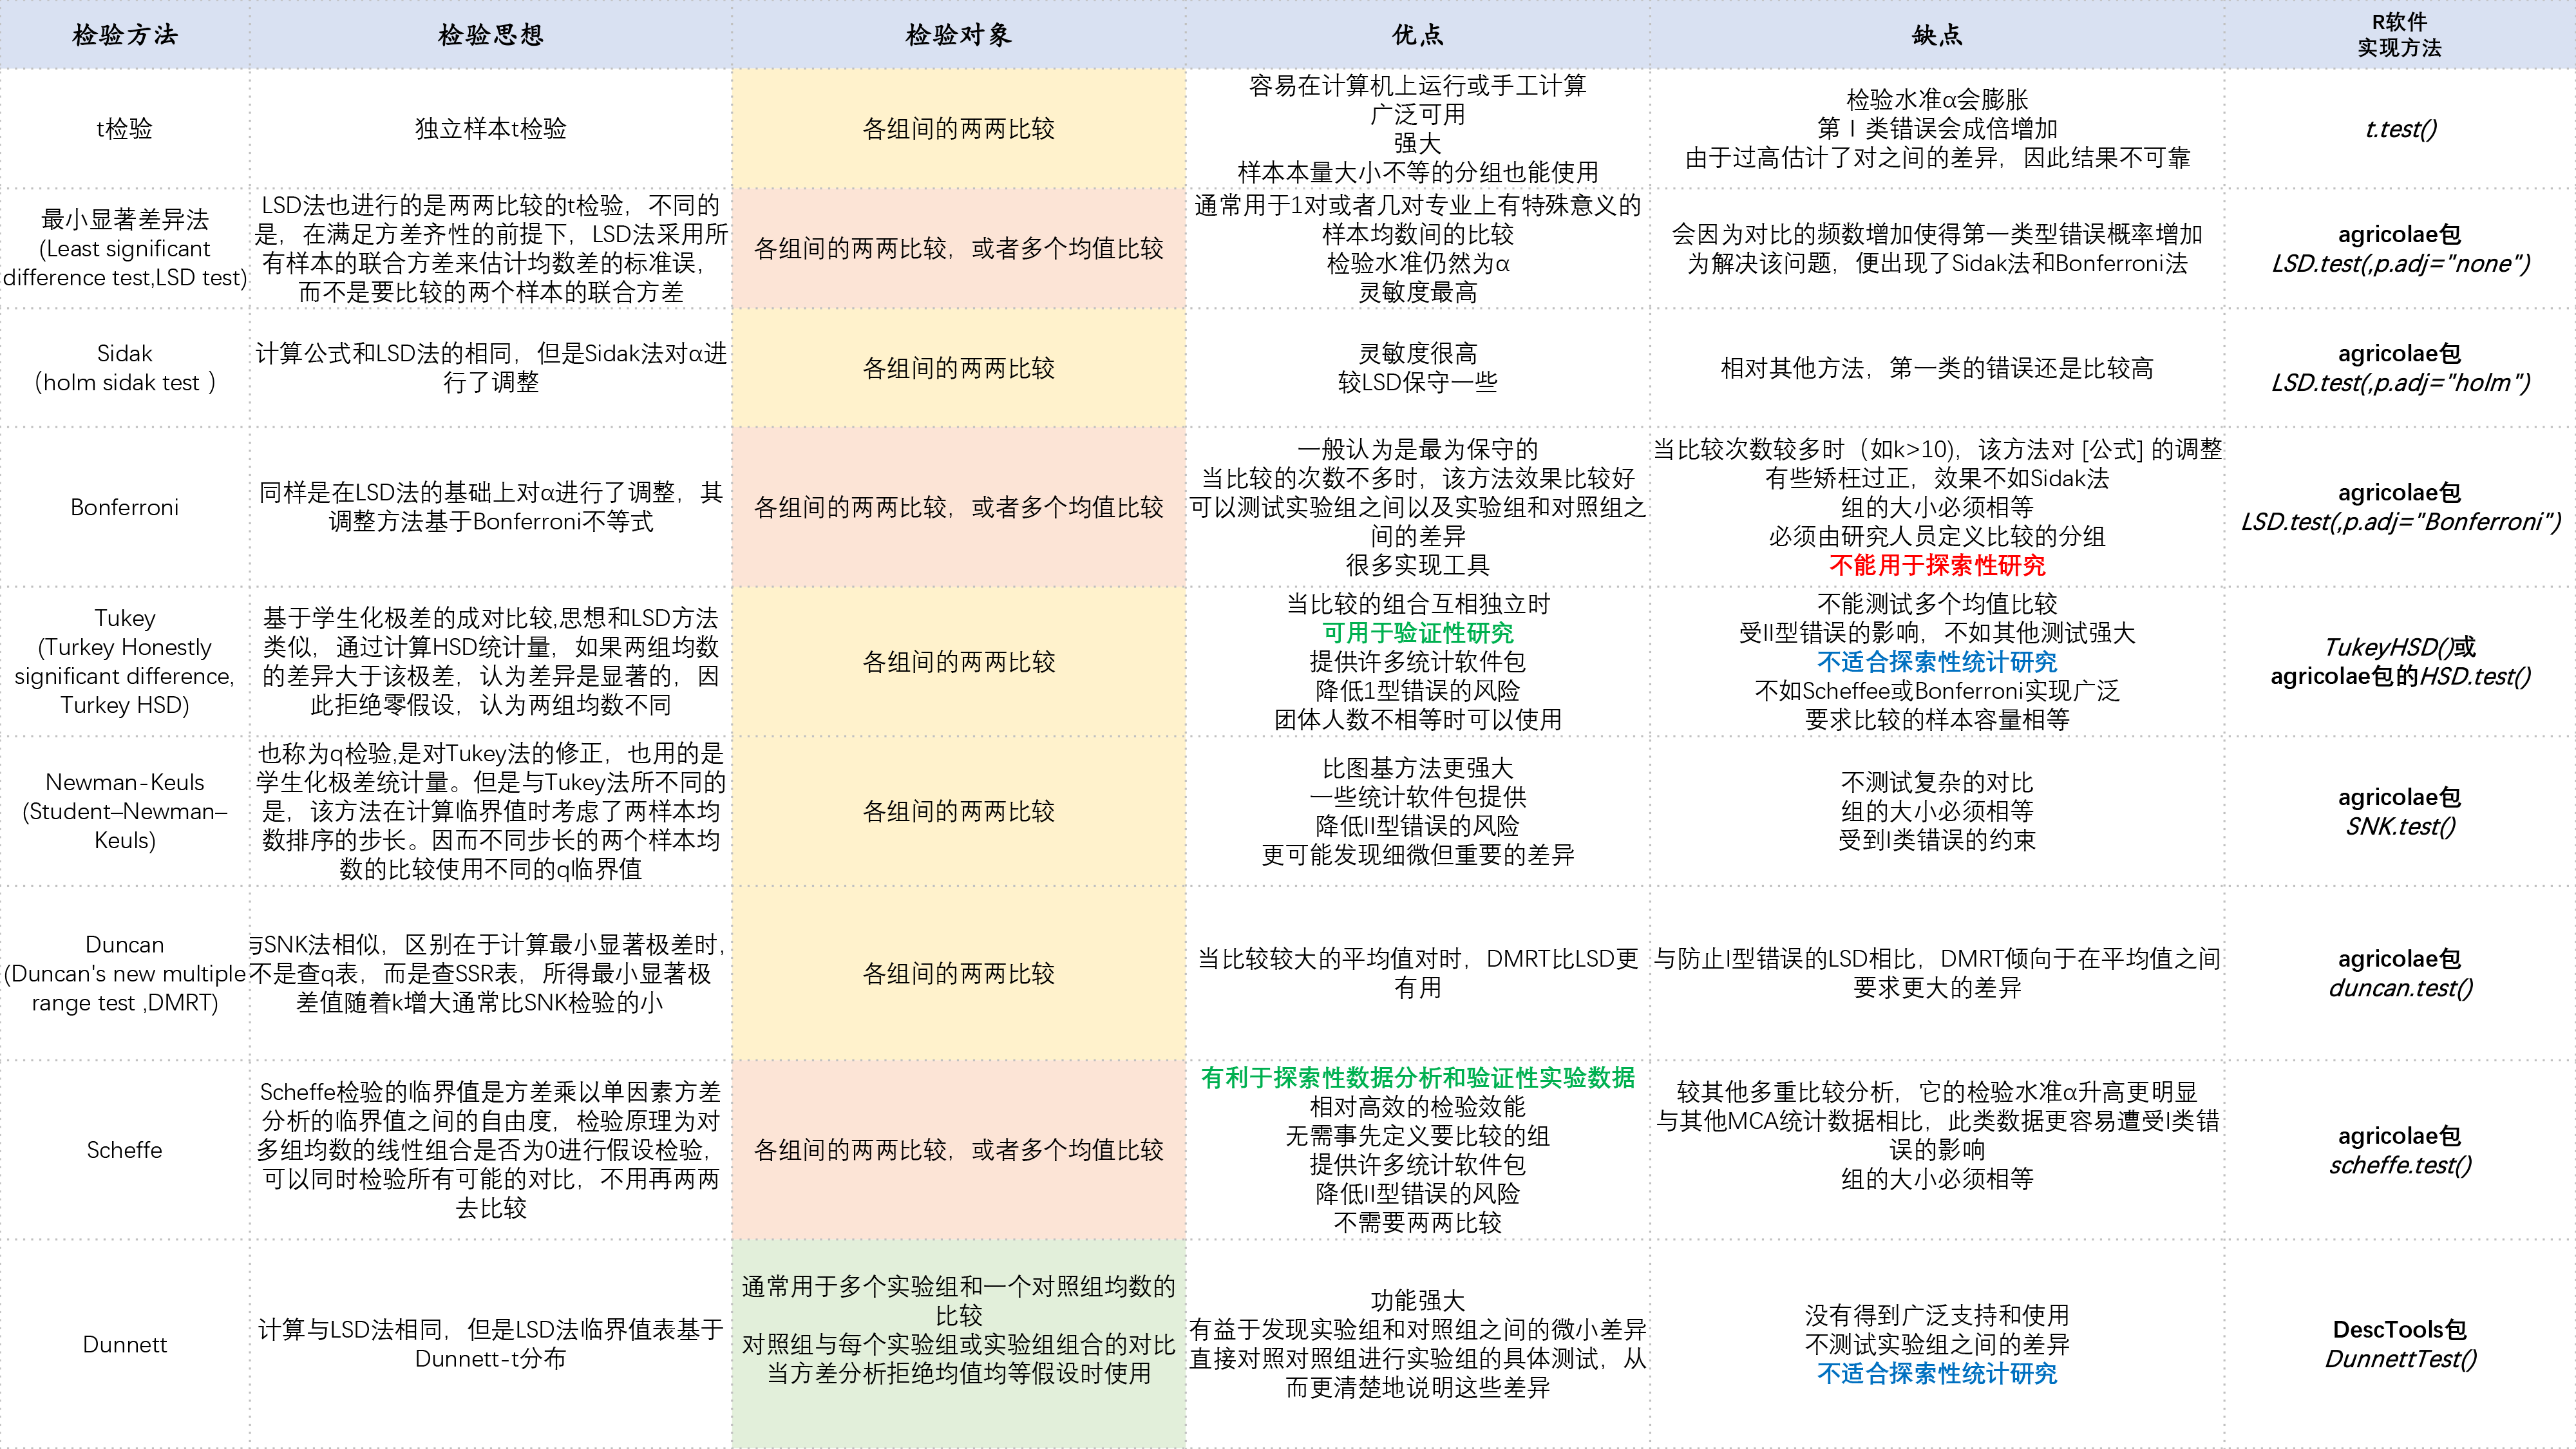
\includegraphics[width=0.95\linewidth]{image/PostHocMethodandR} 

}

\caption{多重比较(Multiple comparison)统计方法的比较}\label{fig:PostHocMethod}
\end{figure}

多重比较(Multiple comparison)在R中几个示例方法,LSD.test(),scheffe.test(),SNK.test(),HSD.test()和TukeyHSD(),DunnettTest(),代码如下:

\begin{Shaded}
\begin{Highlighting}[]
\CommentTok{##案例4-2 }
\CommentTok{#install.packages("pacman")}
\CommentTok{#install.packages("DescTools")}
\CommentTok{#批量加载包}
\NormalTok{pacman}\OperatorTok{::}\KeywordTok{p_load}\NormalTok{(memisc,agricolae,DescTools)}
\CommentTok{#读取数据}
\NormalTok{rdl_sav<-}\KeywordTok{spss.system.file}\NormalTok{(}\StringTok{"ExampleData/SavData4MedSta/Exam04-02.sav"}\NormalTok{)}
\NormalTok{rdl_df<-}\KeywordTok{as.data.frame}\NormalTok{(}\KeywordTok{as.data.set}\NormalTok{(rdl_sav))}
\NormalTok{aov.out =}\StringTok{ }\KeywordTok{aov}\NormalTok{(rdl_df}\OperatorTok{$}\NormalTok{LDL_C }\OperatorTok{~}\StringTok{ }\KeywordTok{as.character}\NormalTok{(rdl_df}\OperatorTok{$}\NormalTok{GROUP))}

\CommentTok{##p.adj=c("none","holm","hommel", "hochberg", "bonferroni", "BH", "BY", "fdr")}
\KeywordTok{LSD.test}\NormalTok{(aov.out,}\StringTok{"as.character(rdl_df$GROUP)"}\NormalTok{, }\DataTypeTok{p.adj=}\StringTok{"bonferroni"}\NormalTok{,}\DataTypeTok{console =}\NormalTok{ T)}
\KeywordTok{plot}\NormalTok{(}\KeywordTok{LSD.test}\NormalTok{(aov.out,}\StringTok{"as.character(rdl_df$GROUP)"}\NormalTok{, }\DataTypeTok{p.adj=}\StringTok{"bonferroni"}\NormalTok{,}\DataTypeTok{console =}\NormalTok{ F))}
\CommentTok{## Study: aov.out ~ "as.character(rdl_df$GROUP)"}
\CommentTok{## }
\CommentTok{## LSD t Test for rdl_df$LDL_C }
\CommentTok{## P value adjustment method: bonferroni }
\CommentTok{## }
\CommentTok{## Mean Square Error:  0.4307502 }
\CommentTok{## }
\CommentTok{## as.character(rdl_df$GROUP),  means and individual ( 95 %) CI}
\CommentTok{## }
\CommentTok{##   rdl_df.LDL_C       std  r      LCL      UCL  Min  Max}
\CommentTok{## 1     3.430333 0.7151247 30 3.193002 3.667664 1.37 4.59}
\CommentTok{## 2     2.715333 0.6381586 30 2.478002 2.952664 1.56 4.32}
\CommentTok{## 3     2.698000 0.4971671 30 2.460669 2.935331 1.68 3.68}
\CommentTok{## 4     1.966333 0.7464421 30 1.729002 2.203664 0.89 3.71}
\CommentTok{## }
\CommentTok{## Alpha: 0.05 ; DF Error: 116}
\CommentTok{## Critical Value of t: 2.684257 }
\CommentTok{## }
\CommentTok{## Minimum Significant Difference: 0.454874 }
\CommentTok{## }
\CommentTok{## Treatments with the same letter are not significantly different.}
\CommentTok{## }
\CommentTok{##   rdl_df$LDL_C groups}
\CommentTok{## 1     3.430333      a}
\CommentTok{## 2     2.715333      b}
\CommentTok{## 3     2.698000      b}
\CommentTok{## 4     1.966333      c}

\CommentTok{#scheffe方法}
\KeywordTok{scheffe.test}\NormalTok{(aov.out,}\StringTok{"as.character(rdl_df$GROUP)"}\NormalTok{,}\DataTypeTok{console =}\NormalTok{ T)}
\CommentTok{## Study: aov.out ~ "as.character(rdl_df$GROUP)"}
\CommentTok{## }
\CommentTok{## Scheffe Test for rdl_df$LDL_C }
\CommentTok{## }
\CommentTok{## Mean Square Error  : 0.4307502 }
\CommentTok{## }
\CommentTok{## as.character(rdl_df$GROUP),  means}
\CommentTok{## }
\CommentTok{##   rdl_df.LDL_C       std  r  Min  Max}
\CommentTok{## 1     3.430333 0.7151247 30 1.37 4.59}
\CommentTok{## 2     2.715333 0.6381586 30 1.56 4.32}
\CommentTok{## 3     2.698000 0.4971671 30 1.68 3.68}
\CommentTok{## 4     1.966333 0.7464421 30 0.89 3.71}
\CommentTok{## }
\CommentTok{## Alpha: 0.05 ; DF Error: 116 }
\CommentTok{## Critical Value of F: 2.682809 }
\CommentTok{## }
\CommentTok{## Minimum Significant Difference: 0.4807537 }
\CommentTok{## }
\CommentTok{## Means with the same letter are not significantly different.}
\CommentTok{## }
\CommentTok{##   rdl_df$LDL_C groups}
\CommentTok{## 1     3.430333      a}
\CommentTok{## 2     2.715333      b}
\CommentTok{## 3     2.698000      b}
\CommentTok{## 4     1.966333      c}

\CommentTok{#SNK方法}
\KeywordTok{SNK.test}\NormalTok{(aov.out,}\StringTok{"as.character(rdl_df$GROUP)"}\NormalTok{,}\DataTypeTok{console =}\NormalTok{ T)}
\CommentTok{## Study: aov.out ~ "as.character(rdl_df$GROUP)"}
\CommentTok{## }
\CommentTok{## Student Newman Keuls Test}
\CommentTok{## for rdl_df$LDL_C }
\CommentTok{## }
\CommentTok{## Mean Square Error:  0.4307502 }
\CommentTok{## }
\CommentTok{## as.character(rdl_df$GROUP),  means}
\CommentTok{## }
\CommentTok{##   rdl_df.LDL_C       std  r  Min  Max}
\CommentTok{## 1     3.430333 0.7151247 30 1.37 4.59}
\CommentTok{## 2     2.715333 0.6381586 30 1.56 4.32}
\CommentTok{## 3     2.698000 0.4971671 30 1.68 3.68}
\CommentTok{## 4     1.966333 0.7464421 30 0.89 3.71}
\CommentTok{## }
\CommentTok{## Alpha: 0.05 ; DF Error: 116 }
\CommentTok{## }
\CommentTok{## Critical Range}
\CommentTok{##         2         3         4 }
\CommentTok{## 0.3356368 0.4023275 0.4417253 }
\CommentTok{## }
\CommentTok{## Means with the same letter are not significantly different.}
\CommentTok{## }
\CommentTok{##   rdl_df$LDL_C groups}
\CommentTok{## 1     3.430333      a}
\CommentTok{## 2     2.715333      b}
\CommentTok{## 3     2.698000      b}
\CommentTok{## 4     1.966333      c}

\CommentTok{#Tukey方法}
\KeywordTok{HSD.test}\NormalTok{(aov.out,}\StringTok{"as.character(rdl_df$GROUP)"}\NormalTok{,}\DataTypeTok{console =}\NormalTok{ T)}
\CommentTok{## Study: aov.out ~ "as.character(rdl_df$GROUP)"}
\CommentTok{## }
\CommentTok{## HSD Test for rdl_df$LDL_C }
\CommentTok{## }
\CommentTok{## Mean Square Error:  0.4307502 }
\CommentTok{## }
\CommentTok{## as.character(rdl_df$GROUP),  means}
\CommentTok{## }
\CommentTok{##   rdl_df.LDL_C       std  r  Min  Max}
\CommentTok{## 1     3.430333 0.7151247 30 1.37 4.59}
\CommentTok{## 2     2.715333 0.6381586 30 1.56 4.32}
\CommentTok{## 3     2.698000 0.4971671 30 1.68 3.68}
\CommentTok{## 4     1.966333 0.7464421 30 0.89 3.71}
\CommentTok{## }
\CommentTok{## Alpha: 0.05 ; DF Error: 116 }
\CommentTok{## Critical Value of Studentized Range: 3.686381 }
\CommentTok{## }
\CommentTok{## Minimun Significant Difference: 0.4417253 }
\CommentTok{## }
\CommentTok{## Treatments with the same letter are not significantly different.}
\CommentTok{## }
\CommentTok{##   rdl_df$LDL_C groups}
\CommentTok{## 1     3.430333      a}
\CommentTok{## 2     2.715333      b}
\CommentTok{## 3     2.698000      b}
\CommentTok{## 4     1.966333      c}

\KeywordTok{TukeyHSD}\NormalTok{(aov.out)}
\CommentTok{##   Tukey multiple comparisons of means}
\CommentTok{##     95% family-wise confidence level}
\CommentTok{## }
\CommentTok{## Fit: aov(formula = rdl_df$LDL_C ~ as.character(rdl_df$GROUP))}
\CommentTok{## }
\CommentTok{## $`as.character(rdl_df$GROUP)`}
\CommentTok{##            diff        lwr        upr     p adj}
\CommentTok{## 2-1 -0.71500000 -1.1567253 -0.2732747 0.0002825}
\CommentTok{## 3-1 -0.73233333 -1.1740587 -0.2906080 0.0001909}
\CommentTok{## 4-1 -1.46400000 -1.9057253 -1.0222747 0.0000000}
\CommentTok{## 3-2 -0.01733333 -0.4590587  0.4243920 0.9996147}
\CommentTok{## 4-2 -0.74900000 -1.1907253 -0.3072747 0.0001302}
\CommentTok{## 4-3 -0.73166667 -1.1733920 -0.2899413 0.0001938}

\CommentTok{#Dunnett,加载DescTools包}
\KeywordTok{DunnettTest}\NormalTok{(rdl_df}\OperatorTok{$}\NormalTok{LDL_C, rdl_df}\OperatorTok{$}\NormalTok{GROUP)}
\CommentTok{##   Dunnett's test for comparing several treatments with a control :  }
\CommentTok{##     95% family-wise confidence level}
\CommentTok{## }
\CommentTok{## $`1`}
\CommentTok{##           diff    lwr.ci     upr.ci    pval    }
\CommentTok{## 2-1 -0.7150000 -1.118364 -0.3116361 0.00015 ***}
\CommentTok{## 3-1 -0.7323333 -1.135697 -0.3289694 9.6e-05 ***}
\CommentTok{## 4-1 -1.4640000 -1.867364 -1.0606361 8.5e-14 ***}
\CommentTok{## }
\CommentTok{## ---}
\CommentTok{## Signif. codes:  0 '***' 0.001 '**' 0.01 '*' 0.05 '.' 0.1 ' ' 1}
\end{Highlighting}
\end{Shaded}

\hypertarget{ux591aux6837ux672cux65b9ux5deeux9f50ux6027ux68c0ux9a8c}{%
\subsection{多样本方差齐性检验}\label{ux591aux6837ux672cux65b9ux5deeux9f50ux6027ux68c0ux9a8c}}

在进行方差分析时要求所对比的各组即各样本的总体方差必须是相等的,这一般需要在作方差分析之前,先对资料的方差齐性进行检验,
特别是在样本方差相差悬殊时,应注意这个问题。对两总体方差进行\protect\hyperlink{ux4e24ux6837ux672cux65b9ux5deeux9f50ux6027ux68c0ux9a8c}{齐性检验}的方法前已介绍。本节介绍多样本(也适用于两样本)方差比较的
Bartlett's 检验和Levene's 检验。

\hypertarget{bartletts-ux68c0ux9a8c}{%
\subsubsection{Bartlett's 检验}\label{bartletts-ux68c0ux9a8c}}

该检验以Maurice Stevenson Bartlett命名的,是基于其抽样分布近似为具有(k-1)自由度的卡方分布的统计量,其中k是随机样本的数量,
其大小可能有所不同,并且每个样本均来自独立的正态分布。 巴特利特的检验对偏离常态很敏感,如果样本来自非正态分布,
那么Bartlett的检验可能就比较差。Levene检验和Brown-Forsythe检验是Bartlett检验的替代方法,对偏离正态性较不敏感。

其统计量和计算公式可以参考《医学统计学》你,或者 \href{https://en.wikipedia.org/wiki/Bartlett\%27s_test}{Wikipedia}。

在R语言中的实现,可以参考下面的代码,以案例4-2数据做测试。根据计算结果,P值=0.1564\textgreater0.1,方差齐性检验的通常按照α=-。1
设置,因此不拒绝\(H_0\),即不拒绝各组之间的方向都相等。

\begin{Shaded}
\begin{Highlighting}[]
\KeywordTok{bartlett.test}\NormalTok{(rdl_df}\OperatorTok{$}\NormalTok{LDL_C,rdl_df}\OperatorTok{$}\NormalTok{GROUP)}
\CommentTok{## }
\CommentTok{##  Bartlett test of homogeneity of variances}
\CommentTok{## }
\CommentTok{## data:  rdl_df$LDL_C and rdl_df$GROUP}
\CommentTok{## Bartlett's K-squared = 5.2192, df = 3, p-value = 0.1564}
\end{Highlighting}
\end{Shaded}

\hypertarget{levenes-ux68c0ux9a8c}{%
\subsubsection{Levene's 检验}\label{levenes-ux68c0ux9a8c}}

Levene's 检验是Bartlett's 检验的替代方法,对样本整体数据不必要是正态分布,对偏离正态性较不敏感。与Levene's 检验相似的
还有Brown--Forsythe检验,两者的区别是用来计算各组的中心取得参数不一样,Brown--Forsythe采用的是中位数(median),Levene's是均值(mean)。

其统计量和计算公式可以参考《医学统计学》你,或者 \href{https://en.wikipedia.org/wiki/Levene\%27s_test}{Wikipedia}。

在R语言中的实现,可以参考下面的代码,以案例4-2数据做测试。根据计算结果,P值=0.1564\textgreater0.1,方差齐性检验的通常按照α=-。1
设置,因此不拒绝\(H_0\),即不拒绝各组之间的方向都相等。

\begin{Shaded}
\begin{Highlighting}[]
\CommentTok{#DescTools包中的LeveneTest()}
\KeywordTok{library}\NormalTok{(DescTools)}
\CommentTok{#Levene's是均值(mean),center = "mean"}
\KeywordTok{LeveneTest}\NormalTok{(rdl_df}\OperatorTok{$}\NormalTok{LDL_C,rdl_df}\OperatorTok{$}\NormalTok{GROUP,}\DataTypeTok{center =} \StringTok{"mean"}\NormalTok{)}
\CommentTok{## }
\CommentTok{## Levene's Test for Homogeneity of Variance (center = "mean")}
\CommentTok{##        Df F value Pr(>F)}
\CommentTok{## group   3  1.6224  0.188}
\CommentTok{##       116    }

\CommentTok{#Brown–Forsythe 是中位数(median),center = "median"}
\KeywordTok{LeveneTest}\NormalTok{(rdl_df}\OperatorTok{$}\NormalTok{LDL_C,rdl_df}\OperatorTok{$}\NormalTok{GROUP,}\DataTypeTok{center =} \StringTok{"median"}\NormalTok{)}
\CommentTok{## }
\CommentTok{## Levene's Test for Homogeneity of Variance (center = "median")}
\CommentTok{##        Df F value Pr(>F)}
\CommentTok{## group   3   1.493 0.2201}
\CommentTok{##       116  }
\end{Highlighting}
\end{Shaded}

\hypertarget{ux7b2cux4e94ux7ae0-ux8ba1ux6570ux8d44ux6599ux7684ux7edfux8ba1ux63cfux8ff0}{%
\section{第五章 计数资料的统计描述}\label{ux7b2cux4e94ux7ae0-ux8ba1ux6570ux8d44ux6599ux7684ux7edfux8ba1ux63cfux8ff0}}

日期: 2020-11-22
作者:wxhyihuan

本章节主要时计数资料相关的概念和统计基础,概念的细节比较多,是后面进行离散变量的统计的基础!可以结合树上的案例,更好的理解和引用概念,此处不累述。

计数资料(Enumeration data,Categorical data),又称定性资料或无序分类资料,是相对于计量资料(Measurement data,又称连续型变量资料,
是指由数值变量的测量值组成的资料)的一个统计概念,是指先将观察单位按其性质或类别分组,然后清点各组观察单位个数所得的资料。
其特点是对每组观察单位主要研究其数量的多少,属非连续性资料。

计数资料常见的数据形式是绝对数,如某病的出院人数、治愈人数等,但绝对数通常不具有可比性,如甲、乙两个医院某病出院人数不同时,
比较两医院该病的死亡人数没有意义,因此需要在绝对数的基础上计算相对数。常用的相对数指标有比、比例和率三种:

\begin{enumerate}
\def\labelenumi{\arabic{enumi}.}
\tightlist
\item
  当比例与时间有关系时称为率(Rate),或称强度相对数;
\item
  当比的分子是分母的一部分时,称为比例(Proportion),或称结构相对数;
\item
  两个有关指标之比称为比(Ratio),或称相对比;
\end{enumerate}

\hypertarget{ux5e38ux7528ux76f8ux5bf9ux6570}{%
\subsection{常用相对数}\label{ux5e38ux7528ux76f8ux5bf9ux6570}}

\hypertarget{ux5f3aux5ea6ux76f8ux5bf9ux6570}{%
\subsubsection{强度相对数}\label{ux5f3aux5ea6ux76f8ux5bf9ux6570}}

强度相对数也称强度相对指标或强度指标,是指同一时期内两个性质不同而又有一定联系的总量指标之比。它可以反映社会经济现象的强度、密度和普遍程度。
其计算公式为:
\[强度相对数(率)=\frac{某时期内发生某现象的观察单位数}{同时期内可能发生某现象的观察单位总数}\times比例基数\]

比例基数主要是调整通过百分/千分/万分等基数,是计算结果能保留适当有效位数,便于阅读。另外就是要注意,不要忽略公式中时间的范畴,所赋予计算结果是
特定观察时期内的,在结果解释时,这个周期(比如年,月,周,天,时)的含义体现。

\hypertarget{ux7ed3ux6784ux76f8ux5bf9ux6570}{%
\subsubsection{结构相对数}\label{ux7ed3ux6784ux76f8ux5bf9ux6570}}

结构相对数又称比重指标或结构相对指标,是在分组情况下,总体内部各组的数值与总体数值相比计算得到的相对数。它反映总体内部的构成情况,
表明总体中各部分所占比重的大小、一般用百分数表示,计算公式为:
\[结构相对数(比例)=\frac{某一构成部分的观察单位数}{同一事物各组成部分的观察单位总数}\times100\%\]

显然,全体内各组结构相对数的总和应为100\%。注意的是,各部分之间是互相影响,某部分的比例既受到自身观察数量变化的影响,
也受到其他部分的观察数量的变化影响。

\hypertarget{ux76f8ux5bf9ux6bd4}{%
\subsubsection{相对比}\label{ux76f8ux5bf9ux6bd4}}

表示两个有关事物指标之比,常以百分数和倍数表示,用以说明一个指标是另一个指标的百分之几或几倍,其计算公式为:
\[相对比(比)=\frac{指标甲}{指标乙}(\times100\%)\]

指标甲乙可以是绝对数,相对数或平均数。

\hypertarget{ux5e94ux7528ux76f8ux5bf9ux6570ux7684ux6ce8ux610fux70b9}{%
\subsubsection{应用相对数的注意点}\label{ux5e94ux7528ux76f8ux5bf9ux6570ux7684ux6ce8ux610fux70b9}}

\begin{enumerate}
\def\labelenumi{\arabic{enumi}.}
\tightlist
\item
  比例不能代替率,即结构相对数不能代替强度相对数
\item
  计算相对数应该有足够的数量
\item
  正确计算合计率 对分组资料计算合计表(或称平均率)时,不能简单的由各组率相加或平均而得,要用合计的有关实际数字进行计算
\item
  注意资料的可比性在比较相对数时,除了要对比的因素(如不同的药物),其余的影响因素应尽可能相同或相近。在临床研究和动物实验时,应遵循随机抽样原则进行分组。下列因素可能影响对比组之间的可比性:
\end{enumerate}

\begin{itemize}
\item
  观察对象是否同质,研究方法是否相同,观察时间是否相等,以及地区、周围环境、风俗习惯和经 济条件是否一致或相近等。
\item
  观察对象内部结构是否相同,若两组资料的年龄、性别等构成不同,可以分别进行同年龄别、同性 别的小组率比较或对总率(合计率)进行\protect\hyperlink{ux7387ux7684ux6807ux51c6ux5316}{标准化}后再作比较。
\end{itemize}

\begin{enumerate}
\def\labelenumi{\arabic{enumi}.}
\setcounter{enumi}{4}
\item
  对比不同时期资料应注意客观条件是否相同,例如,疾病报告制度完善和资料完整的地区或年份,发病率可以``升高'';居民因医疗普及,就诊机会增加,或诊断技术提高,也会引起发病率升高''。因此在分析讨论时,应根据各方面情形全面考虑,慎重对待。
\item
  样本率(或构成比)的抽样误差不能仅凭数字表面相差大小下结论,而应进行样本率(或构成比)差别的假设检验。
\end{enumerate}

\hypertarget{ux7387ux7684ux6807ux51c6ux5316}{%
\subsection{率的标准化}\label{ux7387ux7684ux6807ux51c6ux5316}}

当比较的两组资料,其内部各小组率明显不同,且各小组观察例数的构成比,诸如年龄、性别、工龄、病情轻重、病程长短等也明显不同时,
直接比较两个合计率是不合理的。因为其内部构成不同,往往影响 合计率大小。

因此,一种为在两个以上总率(总均数)进行对比时,消除内部构成不同的影响,采用统一的内部构成,分别计算标准化率(Standardized rate)后再做对比的方法,即为标准化方法(Standardization method),是2014年公布的全科医学与社区卫生名词。标准化法的基本思想是:采用某影响因素的统一标准构成以消除构成不同对合计率的影响,
使通过标准化后的合计率具有可比性。注意的是,它与数据的标准化(Normalization)的概念不同,数据的标准化是将数据按比例缩放,使之落入一个小的特定区间。

\hypertarget{ux6807ux51c6ux5316ux7387ux7684ux8ba1ux7b97}{%
\subsubsection{标准化率的计算}\label{ux6807ux51c6ux5316ux7387ux7684ux8ba1ux7b97}}

标准化法计算的关键是选择统一的标准构成。常用的标准化方法有直接标准化法和间接标准化法,简称直接法和间接法。根据已有资料的条件,采用不同的方法计算标准化率。如对死亡率的年龄构成标准化,若已知年龄别死亡率,可采用直接法;若只 有总死亡数和年龄别人口数而缺乏年龄别死亡率时,或各年龄组人口数较小,年龄别死亡率不稳定时,宜用间接法。

\(N_i\)表示标准年龄别人口数,\(p_i\)为实际年龄别死亡率,N为标准人口众数,选择标准构成的方法通常有三种:

\begin{enumerate}
\def\labelenumi{\arabic{enumi}.}
\item
  两组资料中任选组资料的人口数(或人口构成)作为两者的``共同标准''。这种方法适用于直接法。标准化率的计算公式:
  \[p'=\frac{\sum N_ip_i}{N}\]
\item
  两组资料各部分人口之和组成的人口数(或人口构成)作为两者的``共同标准''。这种方法适用于直接法。标准化率的计算公式:
  \[p'=\sum\left(\frac{N_i}{N}\right)p_i\]
\item
  另外选用一个通用的或便于比较的标准作为两者的``共同标准'',如采用全国、全省或全地区的数据作为标准,这种方法适用于直接法和间接法。标准化率的计算公式:
  \[p'=P\left(\frac{r}{\sum n_iP_i}\right)=P\times SMR\]
\end{enumerate}

\(SMR=r/\sum n_iP_i\)为标准化死亡比(Standardized mortalitu ratio,SMR)。\href{https://baike.baidu.com/item/\%E6\%A0\%87\%E5\%87\%86\%E5\%8C\%96\%E6\%AD\%BB\%E4\%BA\%A1\%E6\%AF\%94}{标准化死亡比}是被标化组实际死亡数与预期死亡数之比,用SMR表示。若SMR\textgreater1,表示被标化人群的死亡率高于标准组;反之,若SMR\textless1,表示被标化人群的死亡率低于标准组。标准化死亡比可反映某一人群与标准人群的人口死亡的相对水平。

\hypertarget{ux52a8ux6001ux6570ux5217ux53caux5176ux6307ux6807ux5206ux6790}{%
\subsection{动态数列及其指标分析}\label{ux52a8ux6001ux6570ux5217ux53caux5176ux6307ux6807ux5206ux6790}}

动态数列(Dynamic series)是一系列按时间顺序排列起来的统计指标(可以为绝对数,相对数或平均 数),用以观察和比较该事物在时间上的变化和发展趋势。常用的动态数列分析指标有:绝对增长量、发展速度与增长速度、平均发展速度与平均增长速度。

\hypertarget{ux7eddux5bf9ux589eux957fux91cf}{%
\subsubsection{绝对增长量}\label{ux7eddux5bf9ux589eux957fux91cf}}

绝对增长量是只事物在一定时间增长的绝对值,可分为:

\begin{itemize}
\tightlist
\item
  累计增长量,即特定时间段内的终末指标值与起始指标值之差;
\item
  逐年增长量,即以年为周期, 今年的指标值与去年的指标值之差。
\end{itemize}

\hypertarget{ux53d1ux5c55ux901fux5ea6ux4e0eux589eux957fux901fux5ea6}{%
\subsubsection{发展速度与增长速度}\label{ux53d1ux5c55ux901fux5ea6ux4e0eux589eux957fux901fux5ea6}}

发展速度与增长速度均为相对比,说明事物在一定时期的速度变化。发展速度表示报告期指标的水 平相当于基期水平的百分之多少或若干倍,根据基期的确定,对发展速度可以计算:

\begin{itemize}
\tightlist
\item
  定基比:即报告期指标与基期指标之比;
\item
  环比:即报告期指标与其前一期指标之比。
\end{itemize}

\hypertarget{ux5e73ux5747ux53d1ux5c55ux901fux5ea6ux4e0eux5e73ux5747ux589eux957fux901fux5ea6}{%
\subsubsection{平均发展速度与平均增长速度}\label{ux5e73ux5747ux53d1ux5c55ux901fux5ea6ux4e0eux5e73ux5747ux589eux957fux901fux5ea6}}

平均发展速度是各环比发展速度的几何均数,说明某事物在一个较长时期中逐期(如逐年)平均发展 的程度。平均增长速度是各环比增长速度的平均数,说明某事物在一个较长时期中逐期平均增长的程度。以\(a_0\)表示基期指标; \(a_n\)为第n期指标,则其计算公式为:

\[\begin{aligned}
平均发展速度 & = \sqrt[n]{a_n/a_0}\\ \\
平均增长速度 & =  平均发展速度 - 1 \\ \\
& = \sqrt[n]{a_n/a_0} -1
\end{aligned}\]

\hypertarget{ux7b2cux516dux7ae0-ux8ba1ux6570ux8d44ux6599ux7684ux7edfux8ba1ux63cfux8ff0}{%
\section{第六章 计数资料的统计描述}\label{ux7b2cux516dux7ae0-ux8ba1ux6570ux8d44ux6599ux7684ux7edfux8ba1ux63cfux8ff0}}

日期: 2020-11-24
作者:wxhyihuan

随机变量有连续型和离散型之分,相应的概率分布就可分为连续型分布(如 u分布、t分布和F分布)和离散型分布,常用的离散型分布有 二项分布、泊松分布,负二项分布,多项分布。

\hypertarget{ux4e8cux9879ux5206ux5e03}{%
\subsection{二项分布}\label{ux4e8cux9879ux5206ux5e03}}

二项分布(Binomial distribution)是\(n\)个独立的 成功/失败(或阴/阳,或是/非) 试验中``成功''的次数\(X\)(即取值{[}0\textasciitilde n{]}之间)的离散概率分布,其中每次试验的``成功''概率为\(p\),记为B(n,p)。这样的\textbf{单次}成功/失败试验又称为伯努利试验,即当\(n = 1\)时,二项分布就是\href{https://zh.wikipedia.org/wiki/\%E4\%BC\%AF\%E5\%8A\%AA\%E5\%88\%A9\%E5\%88\%86\%E5\%B8\%83}{伯努利分布,0-1分布}。二项分布是显著性差异的二项试验的基础。一般地,如果随机变量\(X\)(即取值{[}0\textasciitilde n{]}之间)服从参数为\(n\)和\(p\)的二项分布时,那么\(n\)次试验中正好得到\(x\)次成功的\href{https://zh.wikipedia.org/wiki/\%E6\%A6\%82\%E7\%8E\%87\%E8\%B4\%A8\%E9\%87\%8F\%E5\%87\%BD\%E6\%95\%B0}{概率质量函数}即为:
\[\begin{aligned}
 f(x,n,p)=P(x,n,p) & = \binom{x}{n}p^x(1-p)^{n-x} \\
 & = \frac{n!}{x!(n-x)!}p^x(1-p)^{n-x}, x\in[0,n]
 \end{aligned}\]
P(x)就是\href{https://zh.wikipedia.org/wiki/\%E4\%BA\%8C\%E9\%A1\%B9\%E5\%BC\%8F\%E5\%AE\%9A\%E7\%90\%86}{二项式}\([p+(1-p)]^n\)展开式的通项,\(n!/x!(n-x)!\)为二项系数,且\(\sum_{x=0}^nP(x)=1\)。

\textbf{注意}

对二项分布的资料进行抽样时,如果是有返回(放回)随机抽去n个个体,则依旧是刚才的\(P(x)\)分布函数;如果时无返回(不放回)的随机抽样,自由当n远小于总体个数N(如n \textless{} N/10)时,也可做近似\(P(x)\)分布函数处理。

\textbf{适用的条件}

\begin{enumerate}
\def\labelenumi{\arabic{enumi}.}
\tightlist
\item
  每次实验结果只有发生和不发生两种情形(如成功/失败),且每次实验中,成功/失败事件发生的概率都相同
\item
  重复实验是相互独立
\end{enumerate}

\hypertarget{ux4e8cux9879ux5206ux5e03ux7684ux6027ux8d28}{%
\subsubsection{二项分布的性质}\label{ux4e8cux9879ux5206ux5e03ux7684ux6027ux8d28}}

\hypertarget{ux5747ux6570ux4e0eux6807ux51c6ux5dee}{%
\paragraph{均数与标准差}\label{ux5747ux6570ux4e0eux6807ux51c6ux5dee}}

\textbf{1.``成功''次数的性质}

\textbf{X的总体均数标准差}

在n次独立重复实验中,出现``成功''次数X的总体均数,方差和标准差分别是,
X的总体均数:
\[μ=np\]
X的总方差:
\[σ^2=np(1-p)\]
X的总标准差:
\[σ=\sqrt{np(1-p)}\]

\textbf{率p的总体均数标准差}
在n次独立重复实验中,出现``成功''次数的率p(p=0/n,1/n,2/n\ldots,n/n{]})的总体均数,方差和标准差分别是,
``成功''次数的率p的总体均数:
\[μ_p=p\]

``成功''次数的率p的总方差:
\[σ^2=\frac{p(1-p)}{n}=Var_p\]

``成功''次数的率p的总标准差:
\[σ=\sqrt{\frac{p(1-p)}{n}}=S_p\]

一般的,总体的p往往不知道,因此用样本资料计算样本的``成功''率\(p=X/n\),来计算\(Var_p和S_p\)。

\hypertarget{ux4e8cux9879ux5206ux5e03ux7684ux56feux50cf}{%
\paragraph{二项分布的图像}\label{ux4e8cux9879ux5206ux5e03ux7684ux56feux50cf}}

二项分布的图像偏态主要由p和n决定:

\begin{enumerate}
\def\labelenumi{\arabic{enumi}.}
\tightlist
\item
  当p=0.5时,分布呈对称分布
\item
  当p≠0.5时,图形呈偏态,随着n增大,分布呈逐渐趋向于对称
\item
  当p不太靠近0或1,n-\textgreater∞时,分布呈近似于正态分布
\end{enumerate}

\hypertarget{ux4e0eux5176ux4ed6ux5206ux5e03ux7684ux5173ux7cfb}{%
\paragraph{与其他分布的关系}\label{ux4e0eux5176ux4ed6ux5206ux5e03ux7684ux5173ux7cfb}}

\begin{enumerate}
\def\labelenumi{\arabic{enumi}.}
\tightlist
\item
  伯努利分布是二项分布在n=1时的特殊情况。X\textasciitilde{} B(1,p)与X\textasciitilde{} Bern(p)的意思是相同的。相反,任何二项分布B(n,p)都是n次独立伯努利试验的和,每次试验成功的概率为p。
\item
  泊松近似 当试验的次数n-\textgreater∞,而乘积np固定时,二项分布收敛于\href{https://zh.wikipedia.org/zh-hans/\%E6\%B3\%8A\%E6\%9D\%BE\%E5\%88\%86\%E4\%BD\%88}{泊松分布}。因此参数为λ=np的泊松分布可以作为二项分布B(n,p)的近似,近似成立的前提要求n足够大,而p足够小,np不是很小。
\item
  正态近似 如果n足够大,那么分布的偏度就比较小。在这种情况下,如果使用适当的连续性校正,那么B(n,p)的一个很好的近似是正态分布:N(np,np(1-p))。当n越大(至少20)且p不接近0或1时近似效果更好。不同的经验法则可以用来决定n是否足够大,以及p是否距离0或1足够远,其中一个常用的规则是np和n(1 −p)都必须大于5。
\end{enumerate}

\hypertarget{ux4e8cux9879ux5206ux5e03ux7684ux5e94ux7528}{%
\subsubsection{二项分布的应用}\label{ux4e8cux9879ux5206ux5e03ux7684ux5e94ux7528}}

利用二项分布及其正态近似性,可进行总体率的区间估计和差异推断,也可用于研究非遗传性疾病的家族集聚性和做群检验。对于二分类事物的构成问题,对其中一类的构成比进行统计推断,其方法则类似总体率。

\hypertarget{ux603bux4f53ux7387ux7684ux4f30ux8ba1}{%
\paragraph{总体率的估计}\label{ux603bux4f53ux7387ux7684ux4f30ux8ba1}}

\hypertarget{ux7cbeux786eux6cd5ux76f4ux63a5ux6cd5}{%
\subparagraph{精确法/直接法}\label{ux7cbeux786eux6cd5ux76f4ux63a5ux6cd5}}

对于n≤50的小样本资料,用查表法可以获取百分率的可信区间,即了得到其总体的1-α(α一般取0.05,或0.01)的可信区间。

R语言中的二项分布相关的函数与之前介绍的连续性分布(u分布,t分布和f分布)类似,主要有
\href{https://stat.ethz.ch/R-manual/R-devel/library/stats/html/Binomial.html}{dbinom(),pbinom(),qbinom()和rbinom()}。
用于进行参数估计和假设检验的函数主要有\href{https://stat.ethz.ch/R-manual/R-devel/library/stats/html/binom.test.html}{binom.test()}。

使用《医学统计学》中的 案例6-2 的数据在R中进行二项分布的精确法/查表法分析测试。

\begin{Shaded}
\begin{Highlighting}[]
\NormalTok{n <-}\StringTok{ }\DecValTok{13}
\NormalTok{x <-}\StringTok{ }\DecValTok{6}
\NormalTok{ratio <-}\StringTok{ }\NormalTok{x}\OperatorTok{/}\NormalTok{n}
\KeywordTok{binom.test}\NormalTok{(x, n, }\DataTypeTok{p =} \FloatTok{0.5}\NormalTok{)}
\KeywordTok{binom.test}\NormalTok{(x, n, }\DataTypeTok{p =} \FloatTok{0.5}\NormalTok{, }\DataTypeTok{alternative =} \StringTok{"two.sided"}\NormalTok{, }\DataTypeTok{conf.level =} \FloatTok{0.95}\NormalTok{)}
\CommentTok{##  Exact binomial test}
\CommentTok{## }
\CommentTok{## data:  x and n}
\CommentTok{## number of successes = 6, number of trials = 13, p-value = 1}
\CommentTok{## alternative hypothesis: true probability of success is not equal to 0.5}
\CommentTok{## 95 percent confidence interval:}
\CommentTok{##  0.1922324 0.7486545}
\CommentTok{## sample estimates:}
\CommentTok{## probability of success }
\CommentTok{##              0.4615385 }

\CommentTok{#使用Hmisc包中的binconf()函数}
\CommentTok{#install.packages("Hmisc")}
\KeywordTok{library}\NormalTok{(Hmisc)}
\KeywordTok{binconf}\NormalTok{(x, n, }\DataTypeTok{alpha=}\FloatTok{0.05}\NormalTok{, }\DataTypeTok{method=}\StringTok{"all"}\NormalTok{)}
\CommentTok{##             PointEst     Lower     Upper}
\CommentTok{## Exact      0.4615385 0.1922324 0.7486545}
\CommentTok{## Wilson     0.4615385 0.2320607 0.7085620}
\CommentTok{## Asymptotic 0.4615385 0.1905457 0.7325312}
\end{Highlighting}
\end{Shaded}

\hypertarget{ux6b63ux6001ux8fd1ux4f3cux6cd5}{%
\subparagraph{正态近似法}\label{ux6b63ux6001ux8fd1ux4f3cux6cd5}}

如果n足够大,那么二项分布的偏度就比较小。在这种情况下,如果使用适当的连续性校正,
那么B(n,p)的一个很好的近似是正态分布:N(np,np(1-p)),对应的样本率p也近似正态分布:
N(p,p(1-p)/n)。当n越大(至少20)且p不接近0或1时近似效果更好。
不同的经验法则可以用来决定n是否足够大,以及p是否距离0或1足够远,
其中一个常用的规则是np和n(1 −p)都必须大于5时,可利用样本率p的分布近似正态分布来估计总体的1-α(α=0.05或0.01)的可信区间:
\[(p-u_{a/2}S_p,p+u_{a/2}S_p) ,\]
\(S_p\)为样本资料计算样本的``成功''率\(S_p=\sqrt{{p(1-p)}/{n}},p=X/N\),α=0.05时,\(u_{a/2}=1.96\);α=0.01时,\(u_{a/2}=2.58\)

使用《医学统计学》中的 案例6-3 的数据在R中进行二项分布的正态近似法分析测试。

\begin{Shaded}
\begin{Highlighting}[]
\CommentTok{##用正态分布近似计算}
\NormalTok{n1 <-}\StringTok{ }\DecValTok{100}
\NormalTok{x1 <-}\StringTok{ }\DecValTok{55}
\NormalTok{p1 <-}\StringTok{ }\NormalTok{x1}\OperatorTok{/}\NormalTok{n1}
\NormalTok{S_p1=}\KeywordTok{sqrt}\NormalTok{(p1}\OperatorTok{*}\NormalTok{(}\DecValTok{1}\OperatorTok{-}\NormalTok{p1)}\OperatorTok{/}\NormalTok{n1)}
\NormalTok{p1 }\OperatorTok{+}\StringTok{ }\KeywordTok{c}\NormalTok{(}\OperatorTok{-}\DecValTok{1}\NormalTok{, }\DecValTok{1}\NormalTok{)}\OperatorTok{*}\KeywordTok{qnorm}\NormalTok{(}\FloatTok{0.975}\NormalTok{)}\OperatorTok{*}\NormalTok{S_p1}
\CommentTok{## [1] 0.452493 0.647507}

\CommentTok{##用精确法计算}
\KeywordTok{binom.test}\NormalTok{(x1, n1, }\FloatTok{0.5}\NormalTok{, }\DataTypeTok{alternative=}\StringTok{"two.sided"}\NormalTok{, }\DataTypeTok{conf.level=}\FloatTok{0.95}\NormalTok{)}
\CommentTok{##  Exact binomial test}
\CommentTok{## }
\CommentTok{## data:  x1 and n1}
\CommentTok{## number of successes = 55, number of trials = 100, p-value = 0.3682}
\CommentTok{## alternative hypothesis: true probability of success is not equal to 0.5}
\CommentTok{## 95 percent confidence interval:}
\CommentTok{##  0.4472802 0.6496798}
\CommentTok{## sample estimates:}
\CommentTok{## probability of success }
\CommentTok{##                   0.55 }

\CommentTok{#使用Hmisc包中的binconf()函数}
\KeywordTok{binconf}\NormalTok{(x1, n1, }\DataTypeTok{alpha=}\FloatTok{0.05}\NormalTok{, }\DataTypeTok{method=}\StringTok{"all"}\NormalTok{)}
\CommentTok{##            PointEst     Lower     Upper}
\CommentTok{## Exact          0.55 0.4472802 0.6496798}
\CommentTok{## Wilson         0.55 0.4524460 0.6438546}
\CommentTok{## Asymptotic     0.55 0.4524930 0.6475070}
\end{Highlighting}
\end{Shaded}

\hypertarget{ux6837ux672cux7387ux4e0eux603bux4f53ux7387ux7684ux6bd4ux8f83}{%
\paragraph{样本率与总体率的比较}\label{ux6837ux672cux7387ux4e0eux603bux4f53ux7387ux7684ux6bd4ux8f83}}

\hypertarget{ux76f4ux63a5ux6cd5}{%
\subparagraph{直接法}\label{ux76f4ux63a5ux6cd5}}

使用直接法时,需要注意是单侧检验还是双侧检验。一般的有:

\begin{enumerate}
\def\labelenumi{\arabic{enumi}.}
\tightlist
\item
  单侧检验的情况:

  \begin{itemize}
  \tightlist
  \item
    若是回答``差/低''的问题计算的``成功''\textbf{至多}是k次的概率,即是\(P(X≤k)\);
  \item
    若是回答``优/高''的问题计算的的``成功''\textbf{至少}是k次的概率,即\(P(X≥k)\)的率。
  \end{itemize}
\item
  双侧检验的情况:
  主要是回答``有无差别'',及备择假设是\(p≠p_0\)是否成立,因此计算的是实际样本``成功''k次出现的概率,与更背离原假设的事件出现的概率和。
\end{enumerate}

使用《医学统计学》中的 案例6-4的数据在R中进行二项分布的样本率与总体率的比较的直接法分析测试。

\begin{Shaded}
\begin{Highlighting}[]
\CommentTok{#比较的是至少9次,或者零一对象最多8次的概率,所以:}
\NormalTok{p_}\DecValTok{8}\NormalTok{<-}\KeywordTok{pbinom}\NormalTok{(}\DecValTok{8}\NormalTok{,}\DecValTok{10}\NormalTok{,}\FloatTok{0.55}\NormalTok{)}
\DecValTok{1} \OperatorTok{-}\StringTok{ }\NormalTok{p_}\DecValTok{8}
\CommentTok{#[1] 0.0232571}
\end{Highlighting}
\end{Shaded}

根据计算结果,p(x\textgreater8)=p(x≥9)=0.0232571<0.05,因此拒接原假设\(H_0:p=0.55\),接受\(H_1:p>0.55\)。

使用《医学统计学》中的 案例6-5的数据在R中进行二项分布的样本率与总体率的比较的直接法分析测试。

\begin{Shaded}
\begin{Highlighting}[]
\NormalTok{n2<-}\DecValTok{10}
\NormalTok{x2<-}\DecValTok{9}
\NormalTok{p2<-}\FloatTok{0.6}
\CommentTok{#比较的是至少9次,或者零一对象最多8次的概率,所以:}
\NormalTok{p_}\DecValTok{3}\NormalTok{<-}\KeywordTok{pbinom}\NormalTok{(x2,n2,p2)}
\DecValTok{1} \OperatorTok{-}\StringTok{ }\NormalTok{p_}\DecValTok{3}
\CommentTok{# [1] 0.0232571}
\end{Highlighting}
\end{Shaded}

根据计算结果,p(x\textgreater8)=p(x≥9)=0.0232571<0.05,因此拒接原假设\(H_0:p=0.55\),接受\(H_1:p>0.55\)。

\begin{Shaded}
\begin{Highlighting}[]
\NormalTok{n3<-}\DecValTok{10}
\NormalTok{x3<-}\DecValTok{9}
\NormalTok{p3<-}\FloatTok{0.6}
\CommentTok{#计算的是出现9次的概率:}
\NormalTok{p4<-}\KeywordTok{dbinom}\NormalTok{(x3,n3,p3)}
\CommentTok{# [1] 0.04031078}
\CommentTok{#计算出现更背离原假设的事件及概率,即:}
\NormalTok{p4_}\DecValTok{1}\NormalTok{<-}\KeywordTok{sum}\NormalTok{(}\KeywordTok{dbinom}\NormalTok{(}\DecValTok{0}\OperatorTok{:}\NormalTok{n3,n3,p3)[}\KeywordTok{which}\NormalTok{(}\KeywordTok{dbinom}\NormalTok{(}\DecValTok{0}\OperatorTok{:}\NormalTok{n3,n3,p3)}\OperatorTok{<}\KeywordTok{dbinom}\NormalTok{(x3,n3,p3))])}
\CommentTok{# [1] 0.01834117}
\CommentTok{#双侧检验的p值为:}
\NormalTok{p4}\OperatorTok{+}\NormalTok{p4_}\DecValTok{1}
\CommentTok{# [1] 0.05865196}

\CommentTok{#或者直接用which()函数一并计算}
\KeywordTok{sum}\NormalTok{(}\KeywordTok{dbinom}\NormalTok{(}\DecValTok{0}\OperatorTok{:}\NormalTok{n3,n3,p3)[}\KeywordTok{which}\NormalTok{(}\KeywordTok{dbinom}\NormalTok{(}\DecValTok{0}\OperatorTok{:}\NormalTok{n3,n3,p3)}\OperatorTok{<=}\KeywordTok{dbinom}\NormalTok{(x3,n3,p3))])}
\CommentTok{# [1] 0.05865196}
\end{Highlighting}
\end{Shaded}

根据计算结果,p(x)=0.05865196>0.05,因此不拒接原假设\(H_0:p=0.6\),尚不能认为两种处理的效果不同。

\hypertarget{ux6b63ux6001ux8fd1ux4f3cux6cd5-1}{%
\subparagraph{正态近似法}\label{ux6b63ux6001ux8fd1ux4f3cux6cd5-1}}

当n较大、p和1-p均不太小,如np和n(1-p)均大于5时,利用样本率的分布近似正态分布的原理,
可作样本所在的总体率p与已知总体率\(p_0\)的比较。检验统计量u值的计算公式为:
\[u=\frac{p-p_0}{\sqrt{p_0(1-p_0)/n}}\]

使用《医学统计学》中的 案例6-6的数据在R中进行二项分布的样本率与总体率的比较的正态近似法分析测试。

\begin{Shaded}
\begin{Highlighting}[]
\NormalTok{n4<-}\DecValTok{180}
\NormalTok{x4<-}\DecValTok{117}
\NormalTok{p4<-x4}\OperatorTok{/}\NormalTok{n4}
\NormalTok{p4_}\DecValTok{0}\NormalTok{<-}\FloatTok{0.45}

\NormalTok{u<-(p4}\OperatorTok{-}\NormalTok{p4_}\DecValTok{0}\NormalTok{)}\OperatorTok{/}\KeywordTok{sqrt}\NormalTok{( p4_}\DecValTok{0}\OperatorTok{*}\NormalTok{(}\DecValTok{1}\OperatorTok{-}\NormalTok{p4_}\DecValTok{0}\NormalTok{)}\OperatorTok{/}\NormalTok{n4)}
\CommentTok{# [1] 5.393599}
\CommentTok{#根据正态分布的该v累计分布函数计算出p值}
\KeywordTok{pnorm}\NormalTok{(u,}\DataTypeTok{lower.tail =}\NormalTok{ F)}\OperatorTok{*}\DecValTok{2}
\CommentTok{# [1] 6.906029e-08}

\CommentTok{#整理成函数的形式}
\NormalTok{binom_comp_uAsym<-}\ControlFlowTok{function}\NormalTok{(n1,x1,p0)\{}
\NormalTok{  p1<-x1}\OperatorTok{/}\NormalTok{n1}
\NormalTok{  p_val<-}\KeywordTok{pnorm}\NormalTok{((p1}\OperatorTok{-}\NormalTok{p0)}\OperatorTok{/}\KeywordTok{sqrt}\NormalTok{( p0}\OperatorTok{*}\NormalTok{(}\DecValTok{1}\OperatorTok{-}\NormalTok{p0)}\OperatorTok{/}\NormalTok{n1),}\DataTypeTok{lower.tail =}\NormalTok{ F)}\OperatorTok{*}\DecValTok{2}
  \KeywordTok{return}\NormalTok{( p_val)}
\NormalTok{\}}

\KeywordTok{binom_comp_uAsym}\NormalTok{(n4,x4,p4_}\DecValTok{0}\NormalTok{)}
\CommentTok{# [1] 6.906029e-08}
\end{Highlighting}
\end{Shaded}

根据计算结果,p(x)=6.906029e-08<0.01<0.05,因此拒接原假设\(H_0:p=0.45\),接受\(H_1\),两种处理的效果不同,新的比旧的好。

\hypertarget{ux4e24ux6837ux672cux7387ux7684ux6bd4ux8f83ux6b63ux6001ux8fd1ux4f3c}{%
\paragraph{两样本率的比较(正态近似)}\label{ux4e24ux6837ux672cux7387ux7684ux6bd4ux8f83ux6b63ux6001ux8fd1ux4f3c}}

当n1与n2均较大,p1、p2、1-p1和1-p2均不太小,如n1p1、n1(1-p1)、n2p2、n2(1-p2)均大于5时,可利用样本率的分布
近似正态分布且独立两正态变量之差也服从正态分布的性质,采用近似正态法对两总体率进行统计检验,u的计算公式为:
\[\begin{aligned}
u &= \frac{p_1-p_2}{S_{p_1-p_2}}\\
S_{p_1-p_2} &= \sqrt{\frac{X_1+X_2}{n_1+n_2}(1-\frac{X_1+X_2}{n_1+n_2})(\frac{1}{n_1}+\frac{1}{n_2})}
\end{aligned}\]

使用《医学统计学》中的 案例6-7的数据在R中进行二项分布的样本率与总体率的比较的正态近似法分析测试。

\begin{Shaded}
\begin{Highlighting}[]
\NormalTok{n5<-}\DecValTok{120}
\NormalTok{n6<-}\DecValTok{110}
\NormalTok{x5<-}\DecValTok{36}
\NormalTok{x6<-}\DecValTok{22}

\NormalTok{p5<-x5}\OperatorTok{/}\NormalTok{n5}
\NormalTok{p6<-x6}\OperatorTok{/}\NormalTok{n6}

\NormalTok{S_}\DecValTok{5}\NormalTok{_}\DecValTok{6}\NormalTok{<-}\KeywordTok{sqrt}\NormalTok{((x5}\OperatorTok{+}\NormalTok{x6)}\OperatorTok{/}\NormalTok{(n5}\OperatorTok{+}\NormalTok{n6)}\OperatorTok{*}\NormalTok{(}\DecValTok{1}\OperatorTok{-}\NormalTok{(x5}\OperatorTok{+}\NormalTok{x6)}\OperatorTok{/}\NormalTok{(n5}\OperatorTok{+}\NormalTok{n6))}\OperatorTok{*}\NormalTok{(}\DecValTok{1}\OperatorTok{/}\NormalTok{n5}\OperatorTok{+}\DecValTok{1}\OperatorTok{/}\NormalTok{n6))}
\NormalTok{u<-(p5}\OperatorTok{-}\NormalTok{p6)}\OperatorTok{/}\NormalTok{S_}\DecValTok{5}\NormalTok{_}\DecValTok{6}
\KeywordTok{pnorm}\NormalTok{(u,}\DataTypeTok{lower.tail =}\NormalTok{ F)}\OperatorTok{*}\DecValTok{2}
\CommentTok{# [1] 0.08107076}

\CommentTok{#整理成函数的形式}
\NormalTok{binom_twosamplecomp_uAsym<-}\ControlFlowTok{function}\NormalTok{(n1,x1,n2,x2)\{}
\NormalTok{  p1<-x1}\OperatorTok{/}\NormalTok{n1}
\NormalTok{  p2<-x2}\OperatorTok{/}\NormalTok{n2}
\NormalTok{  S_val<-}\KeywordTok{sqrt}\NormalTok{((x1}\OperatorTok{+}\NormalTok{x2)}\OperatorTok{/}\NormalTok{(n1}\OperatorTok{+}\NormalTok{n2)}\OperatorTok{*}\NormalTok{(}\DecValTok{1}\OperatorTok{-}\NormalTok{(x1}\OperatorTok{+}\NormalTok{x2)}\OperatorTok{/}\NormalTok{(n1}\OperatorTok{+}\NormalTok{n2))}\OperatorTok{*}\NormalTok{(}\DecValTok{1}\OperatorTok{/}\NormalTok{n1}\OperatorTok{+}\DecValTok{1}\OperatorTok{/}\NormalTok{n2))}
\NormalTok{  p_val<-}\KeywordTok{pnorm}\NormalTok{((p1}\OperatorTok{-}\NormalTok{p2)}\OperatorTok{/}\NormalTok{S_val,}\DataTypeTok{lower.tail =}\NormalTok{ F)}\OperatorTok{*}\DecValTok{2}
  \KeywordTok{return}\NormalTok{( p_val)}
\NormalTok{\}}
\KeywordTok{binom_twosamplecomp_uAsym}\NormalTok{(n5,x5,n6,x6)}
\CommentTok{# [1] 0.08107076}
\end{Highlighting}
\end{Shaded}

根据计算结果,p值=0.08107076>0.05>0.01,因此不拒接原假设\(H_0\),尚不能认为两种处理的效果不同。

\hypertarget{ux975eux9057ux4f20ux75beux75c5ux7684ux5bb6ux65cfux805aux96c6ux6027}{%
\paragraph{非遗传疾病的家族聚集性}\label{ux975eux9057ux4f20ux75beux75c5ux7684ux5bb6ux65cfux805aux96c6ux6027}}

非遗传性疾病的家族集聚性(Clustering in familes),系指该疾病的发生在家族成员间是否有传染性,如果没有传染性,则家族成员间的患病是独立的,该疾病无家族集聚性。
否则,家族成员间的患病是非独立的,该疾病存在家族集聚性。

当这种遗传性疾病无家族集聚性时,以家族为样本,在n个成员中,出现X个成员患病的概率分布可认为服从二项分布; 否则,使不服从二项分布。
实际资料与二项分布进行\protect\hyperlink{ux62dfux5408ux4f18ux5ea6ux68c0ux9a8c}{拟合优度(Goodness of fit)的卡方检验}得出p值。

\hypertarget{ux7fa4ux68c0ux9a8c}{%
\paragraph{群检验}\label{ux7fa4ux68c0ux9a8c}}

为了解决检验大批标本的阳性率问题,把N个标本分为n个群,每个群m个标本,即N=n*m。检验每个群是否为阳性群(一旦检测到阳性就停止检测当前群),只有阴性群才需要检测所有标本,可以大大减少检测数目。
记每个标本阳性率为p,则\((1-p)^m\)为m个标本均为阴性的概率,\(1-(1-p)^m\)为一个群为阳性群的概率。
通过阳性群率计算阳性率:假设受检的n个群中,X个群为阳性群,则X/n可作为一个群为阳性群概率的估计值,则有:

\[(1-p)^m=\frac{X}{n}\]

从而估计出:

\[p=1-\sqrt[m]{1-X/n}\]

使用《医学统计学》中的 案例6-9的数据在R中进行二项分布的群检验分析测试。

\begin{Shaded}
\begin{Highlighting}[]
\NormalTok{N<-}\DecValTok{6000}
\NormalTok{n<-}\DecValTok{300}
\NormalTok{m<-}\DecValTok{20}
\NormalTok{X<-}\DecValTok{270}
\DecValTok{1}\OperatorTok{-}\NormalTok{(}\DecValTok{1}\OperatorTok{-}\NormalTok{X}\OperatorTok{/}\NormalTok{n)}\OperatorTok{^}\NormalTok{(}\DecValTok{1}\OperatorTok{/}\NormalTok{m)}
\CommentTok{# [1] 0.1087491}

\CommentTok{#整理成函数的形式}
\NormalTok{binom_commtest<-}\ControlFlowTok{function}\NormalTok{(N,n,m,X)\{}
  \KeywordTok{return}\NormalTok{( }\DecValTok{1}\OperatorTok{-}\NormalTok{(}\DecValTok{1}\OperatorTok{-}\NormalTok{X}\OperatorTok{/}\NormalTok{n)}\OperatorTok{^}\NormalTok{(}\DecValTok{1}\OperatorTok{/}\NormalTok{m))}
\NormalTok{\}}
\KeywordTok{binom_commtest}\NormalTok{(N,n,m,X)}
\CommentTok{# [1] 0.1087491}
\end{Highlighting}
\end{Shaded}

根据计算结果,该地区的钉螺血吸虫的感染率的估计值为10.87\%。

\hypertarget{ux6ccaux677eux5206ux5e03}{%
\subsection{泊松分布}\label{ux6ccaux677eux5206ux5e03}}

泊松分布,也叫Poisson分布,是二项分布的一种\textbf{极端}(即n很大,p很凶啊)情况,已发展为描述小概率事件发生规律的一种重要分布,适合于描述单位时间内随机事件发生的次数的概率分布。如某一服务设施在一定时间内受到的服务请求的次数,电话交换机接到呼叫的次数、汽车站台的候客人数、机器出现的故障数、DNA序列的变异数、放射性原子核的衰变数、发病率低的非传染性疾病发病或人数分布等、单位时间或面积、空间某罕见事物的分布等。如果随机变量X服从总体均数为\(\lambda\)的泊松分布,X取值为0,1,2,···的对应概率质量函数为:
\[P(X)=\frac{e^{-\lambda}\lambda^X}{X!}, X=0,1,2,\dots\]
其中,\(\lambda\)为总体均数,e=2.71828为自然常数,有\(\sum{P(X)}=1\)。

\textbf{适用的条件}
1. 普通性 在充分小的观测单位上X的取值最多为1。简单而言,就是在试验次数n足够大时,每次试验可看作是一个``充分小的观测单位'',且每次试验只会发生两种互斥的可能结果之一(阳性或阴性),这样阳性数X的取值最多为1。
2. 独立增量性 在某个观测单位上的取值与前面各观测单位上的取值无关。简而言之,就是前 面的试验结果不影响下一次的试验结果,各次试验具有独立性。
3. 平稳性 X的取值只与观测单位的大小有关,而与观测单位的位置无关。简单而言,就是每一次 试验阳性事件发生的概率都应相同,为x=/n,这样阳性数 的取值只与重复试验的次数有关,为合计的阳性数,可看作是大量独立试验的总结果。

\hypertarget{ux6ccaux677eux5206ux5e03ux7684ux6027ux8d28}{%
\subsubsection{泊松分布的性质}\label{ux6ccaux677eux5206ux5e03ux7684ux6027ux8d28}}

\hypertarget{ux5747ux6570ux4e0eux6807ux51c6ux5dee-1}{%
\paragraph{均数与标准差}\label{ux5747ux6570ux4e0eux6807ux51c6ux5dee-1}}

\begin{enumerate}
\def\labelenumi{\arabic{enumi}.}
\tightlist
\item
  总体均数\(\lambda\)与总体方差\(\sigma^2\)相等
\item
  n很大p很小,且\(np=\lambda\)为常数时,二项分布近似Poisson分布
\end{enumerate}

\hypertarget{ux6ccaux677eux5206ux5e03ux7684ux56feux50cf}{%
\paragraph{泊松分布的图像}\label{ux6ccaux677eux5206ux5e03ux7684ux56feux50cf}}

\begin{enumerate}
\def\labelenumi{\arabic{enumi}.}
\tightlist
\item
  Poisson分布的图形是右偏分布,均值越大时,其对称性越好
\item
  当\(\lambda≤1\)时,随X取值越大,P(X)取值反而越小;当\(\lambda>1\)时,随X取值越大,P(X)取值先正达后变小;
\item
  当\(\lambda\)为整数时,则在\(X=\lambda\)和\(X=\lambda-1\)处有最大概率值
\item
  \(\lambda\)越大,Poisson分布渐近正态分布,\(\lambda>=20\)时可近似为正态分布
\item
  Possion分布具有可加性(和正态分布类似),但不具有可乘性(可由X取值和均数,方差看出)
\end{enumerate}

\hypertarget{ux6ccaux677eux5206ux5e03ux7684ux5e94ux7528}{%
\subsubsection{泊松分布的应用}\label{ux6ccaux677eux5206ux5e03ux7684ux5e94ux7528}}

利用泊松分布及其正态近似性,可进行总体率的区间估计和差异推断。

\hypertarget{ux603bux4f53ux5747ux6570ux7684ux533aux95f4ux4f30ux8ba1}{%
\paragraph{总体均数的区间估计}\label{ux603bux4f53ux5747ux6570ux7684ux533aux95f4ux4f30ux8ba1}}

利用服从泊松分布的样本资料,可进行总体均属的1-α可信区间,α取值为0.05或0.01。

\hypertarget{ux76f4ux63a5ux6cd5-1}{%
\subparagraph{直接法}\label{ux76f4ux63a5ux6cd5-1}}

对于n≤50的服从泊松分布的小样本资料,用查泊松分布表可以获取百分率的可信区间,即了得到其总体的1-α的可信区间。

R语言中的泊松分布相关的函数与之前介绍的分布(如二项分布,t分布和f分布)类似,主要有
\href{https://www.rdocumentation.org/packages/stats/versions/3.3/topics/Poisson}{dpois(),ppois(),qpois()和rpois()}。
用于进行参数估计和假设检验的函数主要有\href{https://www.rdocumentation.org/packages/stats/versions/3.3/topics/poisson.test}{poisson.test()}。

使用《医学统计学》中的 案例6-10 的数据在R中进行二项分布的精确法/查表法分析测试。

\begin{Shaded}
\begin{Highlighting}[]
\NormalTok{n <-}\StringTok{ }\DecValTok{1}
\NormalTok{x <-}\StringTok{ }\DecValTok{21}
\KeywordTok{poisson.test}\NormalTok{(x, n,}\DataTypeTok{conf.level=}\FloatTok{0.95}\NormalTok{)}
\CommentTok{##  Exact Poisson test}
\CommentTok{## }
\CommentTok{## data:  21 time base: 1}
\CommentTok{## number of events = 21, time base = 1, p-value = 1}
\CommentTok{## alternative hypothesis: true event rate is not equal to 21}
\CommentTok{## 95 percent confidence interval:}
\CommentTok{##  12.99933 32.10073}
\CommentTok{## sample estimates:}
\CommentTok{## event rate }
\CommentTok{##         21 }
\KeywordTok{poisson.test}\NormalTok{(x, n,}\DataTypeTok{conf.level=}\FloatTok{0.99}\NormalTok{)}
\CommentTok{##  Exact Poisson test}
\CommentTok{## }
\CommentTok{## data:  21 time base: 1}
\CommentTok{## number of events = 21, time base = 1, p-value = 1}
\CommentTok{## alternative hypothesis: true event rate is not equal to 21}
\CommentTok{## 99 percent confidence interval:}
\CommentTok{##  11.06923 35.94628}
\CommentTok{## sample estimates:}
\CommentTok{## event rate }
\CommentTok{##         21 }

\CommentTok{#使用exactci包中的poisson.exact()方法,可以使用plot参数绘制出区间图}
\CommentTok{#install.packages("exactci")}
\KeywordTok{library}\NormalTok{(}\StringTok{"exactci"}\NormalTok{)}
\KeywordTok{poisson.exact}\NormalTok{(}\DecValTok{21}\NormalTok{, }\DataTypeTok{plot=}\NormalTok{T, }\DataTypeTok{conf.level=}\FloatTok{0.95}\NormalTok{)}
\KeywordTok{poisson.exact}\NormalTok{(}\DecValTok{21}\NormalTok{, }\DataTypeTok{plot=}\NormalTok{T, }\DataTypeTok{conf.level=}\FloatTok{0.99}\NormalTok{)}
\end{Highlighting}
\end{Shaded}

根据计算结果,95\%和99\%的可信区间分别是(12.99933,32.10073)和(11.06923,35.94628)。

\hypertarget{ux6b63ux6001ux8fd1ux4f3cux6cd5-2}{%
\subparagraph{正态近似法}\label{ux6b63ux6001ux8fd1ux4f3cux6cd5-2}}

对于n>50的服从泊松分布的样本资料,可以采用正态近似法获取百分率的可信区间,即了得到其总体的1-α的可信区间。
\[(X-u_{\alpha/2}\sqrt{X},X+u_{\alpha/2}\sqrt{X})\]

使用《医学统计学》中的 案例6-11 的数据在R中进行泊松分布的正态近似法分析测试。

\begin{Shaded}
\begin{Highlighting}[]
\NormalTok{x<-}\DecValTok{68}
\NormalTok{alpha1<-}\FloatTok{0.05}
\NormalTok{alpha2<-}\FloatTok{0.01}

\NormalTok{posi_uAsym<-}\ControlFlowTok{function}\NormalTok{(X,alpha) \{}
\NormalTok{  Low<-X}\OperatorTok{-}\KeywordTok{qnorm}\NormalTok{(alpha}\OperatorTok{/}\DecValTok{2}\NormalTok{)}\OperatorTok{*}\KeywordTok{sqrt}\NormalTok{(X)}
\NormalTok{  Up<-X}\OperatorTok{+}\KeywordTok{qnorm}\NormalTok{(alpha}\OperatorTok{/}\DecValTok{2}\NormalTok{)}\OperatorTok{*}\KeywordTok{sqrt}\NormalTok{(X)}
  \KeywordTok{return}\NormalTok{(}\KeywordTok{list}\NormalTok{(Low,Up))}
\NormalTok{\}}

\KeywordTok{posi_uAsym}\NormalTok{(x,alpha1)}
\CommentTok{# 84.16228}
\CommentTok{# 51.83772}
\KeywordTok{posi_uAsym}\NormalTok{(x,alpha2)}
\CommentTok{# 89.24083}
\CommentTok{# 46.75917}
\end{Highlighting}
\end{Shaded}

\hypertarget{ux6837ux672cux5747ux6570ux4e0eux603bux4f53ux5747ux6570ux7684ux6bd4ux8f83}{%
\paragraph{样本均数与总体均数的比较}\label{ux6837ux672cux5747ux6570ux4e0eux603bux4f53ux5747ux6570ux7684ux6bd4ux8f83}}

\hypertarget{ux76f4ux63a5ux6cd5-2}{%
\subparagraph{直接法}\label{ux76f4ux63a5ux6cd5-2}}

当总体均数\(\lambda\)\textless20\(时,可采用直接计算概率的方式对样本均数与已知总体均数间的差别进行有无 统计学意义的比较。如用于发病率很低的非传染性疾病,则是对以样本计数X为代表的总体率p与已知的总 体率\)p\_0\$,是否有差别进行推断。

使用《医学统计学》中的 案例6-12 的数据在R中进行样本均数与总体均数的泊松分布-直接法分析测试。

\begin{Shaded}
\begin{Highlighting}[]
\NormalTok{p0<-}\FloatTok{0.008}
\NormalTok{n<-}\DecValTok{120}
\NormalTok{X<-}\DecValTok{4}
\NormalTok{lambda<-n}\OperatorTok{*}\NormalTok{p0}

\CommentTok{#计算不小于4的泊松分布概率和}
\KeywordTok{ppois}\NormalTok{(X}\DecValTok{-1}\NormalTok{, }\DataTypeTok{lambda=}\NormalTok{lambda,}\DataTypeTok{lower.tail =}\NormalTok{ F)}
\CommentTok{#或者}
\DecValTok{1}\OperatorTok{-}\KeywordTok{sum}\NormalTok{(}\KeywordTok{dpois}\NormalTok{(}\DecValTok{0}\OperatorTok{:}\NormalTok{(X}\DecValTok{-1}\NormalTok{), }\DataTypeTok{lambda=}\NormalTok{lambda))}
\CommentTok{# [1] 0.01663305}
\end{Highlighting}
\end{Shaded}

根据计算结果,p值为0.0166\textless0.05,按照α=0.05的检验水准,拒绝原假设\(H_0\),接受\(H_1\),即认为母亲吸烟会增大小孩的先天心脏病危险。

\hypertarget{ux6b63ux6001ux8fd1ux4f3cux6cd5-3}{%
\subparagraph{正态近似法}\label{ux6b63ux6001ux8fd1ux4f3cux6cd5-3}}

当总体均数\(\lambda\)≥20\$时,可采用正态近似法的方式对样本均数与已知总体均数间的差别进行有无
统计学意义的比较,检验统计量u值的计算公式为:
\[u=\frac{X-\lambda}{\sqrt{\lambda}}\]

使用《医学统计学》中的 案例6-13的数据在R中进行样本率与总体率的比较的泊松分布-正态近似法分析测试。

\begin{Shaded}
\begin{Highlighting}[]
\NormalTok{p0<-}\FloatTok{0.003}
\NormalTok{n=}\DecValTok{25000}
\NormalTok{X<-}\DecValTok{123}

\NormalTok{posi_comp_uAsym<-}\ControlFlowTok{function}\NormalTok{(n,X,p0) \{}
\NormalTok{  u_val<-(X}\OperatorTok{-}\NormalTok{n}\OperatorTok{*}\NormalTok{p0)}\OperatorTok{/}\KeywordTok{sqrt}\NormalTok{(n}\OperatorTok{*}\NormalTok{p0)}
  \CommentTok{#print (u_val)}
\NormalTok{  p_val<-}\KeywordTok{pnorm}\NormalTok{(u_val,}\DataTypeTok{lower.tail =}\NormalTok{ F)}\OperatorTok{*}\DecValTok{2}
  \KeywordTok{return}\NormalTok{(p_val)}
\NormalTok{\}}

\KeywordTok{posi_comp_uAsym}\NormalTok{(n,X,p0)}
\CommentTok{# [1] 2.980768e-08}
\end{Highlighting}
\end{Shaded}

根据计算结果,p值为2.980768e-08\textless0.05,按照α=0.05的检验水准,拒绝原假设\(H_0\),接受\(H_1\)。

\hypertarget{ux4e24ux6837ux672cux5747ux6570ux7684ux6bd4ux8f83ux6b63ux6001ux8fd1ux4f3c}{%
\paragraph{两样本均数的比较(正态近似)}\label{ux4e24ux6837ux672cux5747ux6570ux7684ux6bd4ux8f83ux6b63ux6001ux8fd1ux4f3c}}

对服从 Poisson 分布的样本,其样本计数可看作是样本均数。两个样本均数的比较,目的在于推断两样
本所代表的两总体均数是否有差别。设两个样本计数分别为\(X_1\)和\(X_2\),可利用正态近似法进行比较,有下面两种情况:

\textbf{两个样本的观察单位数相等,即\(n_1=n_2\)}
当\(X_1+X_2≥20\)时:
\[u=\frac{X_1-X_2}{\sqrt{X_1+X_2}}\]
当\(5<X_1+X_2<20\)时:
\[u=\frac{|X_1-X_2|-1}{\sqrt{X_1+X_2}}\]

\textbf{两个样本的观察单位数不相等,即\(n_1≠n_2\)}:
当\(X_1+X_2≥20\)时:
\[u=\frac{\bar{X_1}-\bar{X_2}}{\sqrt{X_1/n_1^2+X_2/n_2^2}}\]
当\(5<X_1+X_2<20\)时:
\[u=\frac{|\bar{X_1}-\bar{X_2}|-1}{\sqrt{X_1/n_1^2+X_2/n_2^2}}\]
其中的\(\bar{X_1}\)和\bar\{X\_2\}分别是\(X_1/n_1\)和\(X_2/n_2\)。

使用《医学统计学》中的 案例6-14,6-15的数据在R中进行两样本均数的比较的泊松分布-正态近似法分析测试。

\begin{Shaded}
\begin{Highlighting}[]
\NormalTok{n1<-}\DecValTok{1}
\NormalTok{n2<-}\DecValTok{1}
\NormalTok{x1<-}\DecValTok{4}
\NormalTok{x2<-}\DecValTok{7}

\NormalTok{posi_twosamplecom_uAsym <-}\ControlFlowTok{function}\NormalTok{(n1,n2,x1,x2)\{}
\NormalTok{  u_val<-}\OtherTok{NULL}
  \ControlFlowTok{if}\NormalTok{(n1}\OperatorTok{==}\NormalTok{n2)\{}
    \ControlFlowTok{if}\NormalTok{((x1}\OperatorTok{+}\NormalTok{x2)}\OperatorTok{>=}\DecValTok{20}\NormalTok{)}
\NormalTok{      u_val<-(x1}\OperatorTok{-}\NormalTok{x2)}\OperatorTok{/}\KeywordTok{sqrt}\NormalTok{(x1}\OperatorTok{+}\NormalTok{x2)}
    \ControlFlowTok{else} \ControlFlowTok{if}\NormalTok{ (}\DecValTok{5}\OperatorTok{<}\NormalTok{(x1}\OperatorTok{+}\NormalTok{x2) }\OperatorTok{&&}\StringTok{ }\NormalTok{(x1}\OperatorTok{+}\NormalTok{x2)}\OperatorTok{<}\DecValTok{20}\NormalTok{) }
\NormalTok{      u_val<-(}\KeywordTok{abs}\NormalTok{(x1}\OperatorTok{-}\NormalTok{x2)}\OperatorTok{-}\DecValTok{1}\NormalTok{)}\OperatorTok{/}\KeywordTok{sqrt}\NormalTok{(x1}\OperatorTok{+}\NormalTok{x2)}
\NormalTok{  \}}\ControlFlowTok{else}\NormalTok{\{}
\NormalTok{    x1m<-x1}\OperatorTok{/}\NormalTok{n1}
\NormalTok{    x2m<-x2}\OperatorTok{/}\NormalTok{n2}
     \ControlFlowTok{if}\NormalTok{((x1}\OperatorTok{+}\NormalTok{x2)}\OperatorTok{>=}\DecValTok{20}\NormalTok{)}
\NormalTok{      u_val<-(x1m}\OperatorTok{-}\NormalTok{x2m)}\OperatorTok{/}\KeywordTok{sqrt}\NormalTok{(x1}\OperatorTok{/}\NormalTok{n1}\OperatorTok{^}\DecValTok{2}\OperatorTok{+}\NormalTok{x2}\OperatorTok{/}\NormalTok{n2}\OperatorTok{^}\DecValTok{2}\NormalTok{)}
    \ControlFlowTok{else} \ControlFlowTok{if}\NormalTok{ (}\DecValTok{5}\OperatorTok{<}\NormalTok{(x1}\OperatorTok{+}\NormalTok{x2) }\OperatorTok{&&}\StringTok{ }\NormalTok{(x1}\OperatorTok{+}\NormalTok{x2)}\OperatorTok{<}\DecValTok{20}\NormalTok{) }
\NormalTok{      u_val<-(}\KeywordTok{abs}\NormalTok{(x1m}\OperatorTok{-}\NormalTok{x2m)}\OperatorTok{-}\DecValTok{1}\NormalTok{)}\OperatorTok{/}\KeywordTok{sqrt}\NormalTok{(x1}\OperatorTok{/}\NormalTok{n1}\OperatorTok{^}\DecValTok{2}\OperatorTok{+}\NormalTok{x2}\OperatorTok{/}\NormalTok{n2}\OperatorTok{^}\DecValTok{2}\NormalTok{)}
\NormalTok{  \}}
  \CommentTok{#print(u_val)}
  \KeywordTok{return}\NormalTok{(}\KeywordTok{pnorm}\NormalTok{(u_val,}\DataTypeTok{lower.tail =}\NormalTok{ F)}\OperatorTok{*}\DecValTok{2}\NormalTok{)}
\NormalTok{\}}
\CommentTok{#案例6-14}
\KeywordTok{posi_twosamplecom_uAsym}\NormalTok{(n1,n2,x1,x2)}
\CommentTok{# [1] 0.5464936}

\CommentTok{#案例6-15}
\KeywordTok{posi_twosamplecom_uAsym}\NormalTok{(}\DecValTok{4}\NormalTok{,}\DecValTok{3}\NormalTok{,}\DecValTok{32}\NormalTok{,}\DecValTok{12}\NormalTok{)}
\CommentTok{# [1] 0.02845974}
\end{Highlighting}
\end{Shaded}

根据计算结果,案例6-14的p值为0.5464936\textgreater0.05,按照α=0.05的检验水准,不拒绝原假设\(H_0\)。

根据计算结果,案例6-15的p值为0.02845974\textless0.05,按照α=0.05的检验水准,拒绝原假设\(H_0\),接受\(H_1H_1\)。

\hypertarget{ux8d1fux4e8cux9879ux5206ux5e03}{%
\subsection{负二项分布}\label{ux8d1fux4e8cux9879ux5206ux5e03}}

负二项分布是统计学上一种描述在一系列独立同分布的伯努利试验中,
``成功''(或``失败'')次数到达指定次数(记为r)时``失败''(或``成功'')的次数(记为k)的离散概率分布。
根据参数r是否为整数,负二项分布有两种,当r为整数时,也称为帕斯卡分布(Pascal distribution);
当r为延申到非整数时,也称为波利亚分布(Polya distribution)。
这里仅考虑r为整数时,也就是帕斯卡分布的情况,其定义有下面两种形式:

\begin{enumerate}
\def\labelenumi{\arabic{enumi}.}
\tightlist
\item
  在一系列伯努利试验中,失败次数到达指定次数时,成功次数的离散概率分布
\item
  在一系列伯努利试验中,成功次数到达指定次数(指定值,记为r)时,失败次数(观察变量,记为k)的离散概率分布
\end{enumerate}

这两种定义只是将``成功''和``失败''对调,其本质上没差别。一般的,为方便与之前的分布概念保持一直,便于理解,
都采用第二种形式。记r是成功的次数,为固定值;k是失败的次数,为自变量;p是伯努利试验成功的概率,失败概率则为1-p;因此下面将以第二种形式为例。
其概率质量函数为:
\[\begin{aligned}
f(k,r,p)=P(k,r,p)=p(x=k) & = \binom{k+r-1}{r-1}p^r(1-p)^k\\
& = \frac{(k+r-1)!}{k!(r-1)!}p^r(1-p)^k ,k=0,1,2,\dots\\
& = (-1)^k\binom{-r}{k}p^r(1-p)^k
\end{aligned}\]
该表达式可以写成带负值参数\((-1)^k\)的二项系数的形式,解释了``负二项''名称的来源。

\textbf{注意}
有些资料对负二项分布的定义可能与这里的资料略有不同。最常见的变化是随机变量X计算不同的东西。
这些变化可以在这里的\href{https://en.wikipedia.org/wiki/Negative_binomial_distribution\#Alternative_formulations}{表格}中看到。

\hypertarget{ux8d1fux4e8cux9879ux5206ux5e03ux7684ux6027ux8d28}{%
\subsubsection{负二项分布的性质}\label{ux8d1fux4e8cux9879ux5206ux5e03ux7684ux6027ux8d28}}

\hypertarget{ux5747ux6570ux4e0eux6807ux51c6ux5dee-2}{%
\paragraph{均数与标准差}\label{ux5747ux6570ux4e0eux6807ux51c6ux5dee-2}}

负二项分布的概率分布依赖参数p和r,其总体的均值和方差,标准差为:

X的总体均数:
\[μ=r\frac{1-p}{p}\]
X的方差:
\[σ^2=r\frac{1-p}{p^2}=\frac{μ}{p}=μ+μ^2/r\]
X的标准差:
\[σ=\frac{\sqrt{r(1-p)}}{p}\]

\hypertarget{ux8d1fux4e8cux9879ux5206ux5e03ux7684ux56feux50cf}{%
\paragraph{负二项分布的图像}\label{ux8d1fux4e8cux9879ux5206ux5e03ux7684ux56feux50cf}}

\begin{enumerate}
\def\labelenumi{\arabic{enumi}.}
\tightlist
\item
  负二项分布的图像偏态主要由p和n决定:
\item
  负二项分布 与 二项分布 的区别在于:``二项分布''是固定试验总次数N的独立试验中,成功次数k的分布;而``负二项分布''是所有到r次成功时即终止的独立试验中,失败次数k的分布。
\item
  正态近似 如果n足够大,那么分布的偏度就比较小
\end{enumerate}

\hypertarget{ux4e0eux5176ux4ed6ux5206ux5e03ux7684ux5173ux7cfb-1}{%
\paragraph{与其他分布的关系}\label{ux4e0eux5176ux4ed6ux5206ux5e03ux7684ux5173ux7cfb-1}}

\begin{enumerate}
\def\labelenumi{\arabic{enumi}.}
\tightlist
\item
  负二项分布 与 二项分布 的区别在于:``二项分布''是固定试验总次数N的独立试验中,成功次数k的分布;而``负二项分布''是所有到r次成功时即终止的独立试验中,失败次数k的分布。
\item
  当r=1时,负二项分布退化为\href{https://zh.wikipedia.org/zh-cn/\%E5\%B9\%BE\%E4\%BD\%95\%E5\%88\%86\%E4\%BD\%88}{几何分布}
\end{enumerate}

\hypertarget{ux8d1fux4e8cux9879ux5206ux5e03ux7684ux53c2ux6570ux4f30ux8ba1}{%
\subsubsection{负二项分布的参数估计}\label{ux8d1fux4e8cux9879ux5206ux5e03ux7684ux53c2ux6570ux4f30ux8ba1}}

负二项分布有两个参数即u和r。r值越大,分布的方差与均数的比值就越接近 1;
而r值越小,分布的方差与均数的比值就越大。为此,可以用r值的大小来衡量
分布的离散程度即聚集 趋向的程度,常称为聚集指数(Cluster index)。

负二项分布的参数一般可用样本均数\(\bar{k}\)作为其估计值,即\(u=\bar{k}\),
但参数r的估计就复杂一些。关于r的估计方法常用的有矩法、零频数法和最大似然法等。

\textbf{矩法}
用样本的均数\(\bar{k}\)和方差\(S^2\)分别作为负二项分布的均数μ和方差\(\sigma^2\)的估计值,
可以利用公式:
\[\bar{r}=\frac{\bar{k}^2}{S^2-\bar{k}}, \bar{k}=\sum{fk}/N, S^2=(\sum{fk^2}-(\sum{fk})^2/N)/(N-1)\]
式子中的\(f\)为样本观察到的``失败''数k所对应的频数,N为观察但总数。

使用《医学统计学》中的 案例6-16 的数据在R中进行矩法估计聚集指数r(Cluster index)分析测试。

\begin{Shaded}
\begin{Highlighting}[]
\NormalTok{arr1<-}\KeywordTok{array}\NormalTok{(}\DataTypeTok{dim=}\KeywordTok{c}\NormalTok{(}\DecValTok{2}\NormalTok{,}\DecValTok{7}\NormalTok{))}
\NormalTok{arr1[}\DecValTok{1}\NormalTok{,]<-}\DecValTok{0}\OperatorTok{:}\DecValTok{6}
\NormalTok{arr1[}\DecValTok{2}\NormalTok{,]<-}\KeywordTok{c}\NormalTok{(}\DecValTok{30}\NormalTok{,}\DecValTok{14}\NormalTok{,}\DecValTok{8}\NormalTok{,}\DecValTok{4}\NormalTok{,}\DecValTok{2}\NormalTok{,}\DecValTok{0}\NormalTok{,}\DecValTok{2}\NormalTok{)}

\NormalTok{negbino_jufa_restim<-}\ControlFlowTok{function}\NormalTok{(k_val,freq)\{}
\NormalTok{  N<-}\KeywordTok{sum}\NormalTok{(freq)}
\NormalTok{  sum_fk<-}\KeywordTok{sum}\NormalTok{(k_val }\OperatorTok{*}\StringTok{ }\NormalTok{freq)}
\NormalTok{  sum_fkk<-}\KeywordTok{sum}\NormalTok{(k_val}\OperatorTok{^}\DecValTok{2} \OperatorTok{*}\StringTok{ }\NormalTok{freq)}
\NormalTok{  mean_val<-sum_fk}\OperatorTok{/}\NormalTok{N}
\NormalTok{  var_val<-(sum_fkk}\OperatorTok{-}\NormalTok{sum_fk}\OperatorTok{^}\DecValTok{2}\OperatorTok{/}\NormalTok{N)}\OperatorTok{/}\NormalTok{(N}\DecValTok{-1}\NormalTok{)}
  \CommentTok{#print(paste(N, mean_val ,var_val, sep = "   "))}
\NormalTok{  r_estim<-mean_val}\OperatorTok{^}\DecValTok{2}\OperatorTok{/}\NormalTok{(var_val}\OperatorTok{-}\NormalTok{mean_val)}
  \KeywordTok{return}\NormalTok{(r_estim)}
\NormalTok{\}}

\KeywordTok{negbino_jufa_restim}\NormalTok{(arr1[}\DecValTok{1}\NormalTok{,],arr1[}\DecValTok{2}\NormalTok{,])}
\CommentTok{# [1] 1.033333}
\end{Highlighting}
\end{Shaded}

\textbf{零频数法}

零频法(Zero frequency method)是利用样本计数k=0时,所对应的频数\(f_0\)占观察单位总数的比例,即
\(f_0/N\)来估计r值,即求解满足下面的方程的r值:
\[r\lg(1+\bar{k}/r)=\lg(N/f_0)\]
\emph{使用此方法要注意满足适当的条件。}
- \(\frac{f_0}{N}>\frac{1}{3}\)
- 当\(\bar{r}<10\)时,还必须有充分的\(f_0\)项,以满足不等式:\((\bar{r}_0.17)(\frac{f_0}{N}-0.32)>0.20\)
- 往往需要使用线性内插法(Linear interpolation method)才能求得r的估计值。

\textbf{最大似然法}

最大似然法(Maximum likelihood method)是满足下面是指的z=0的r值:
\[z=\sum_{k=0}^m\frac{A_k}{r+k}-N\ln(1+\bar{k}/r)\]
公式中\(m=k_max\),即样本计数k所取得的最大值;\(A_k=\sum_{i=k+1}^mf_i\),即样本中所有计数发育k的频数之和。

需要使用线性内插法(Linear interpolation method)才能求得r的估计值,该方法的估计更为精确,但是计算很复杂。

\hypertarget{ux8d1fux4e8cux9879ux5206ux5e03ux7684ux5e94ux7528}{%
\subsubsection{负二项分布的应用}\label{ux8d1fux4e8cux9879ux5206ux5e03ux7684ux5e94ux7528}}

R语言中的二项分布相关的函数与之前介绍的连续性分布(u分布,t分布和f分布)类似,主要有
\href{https://stat.ethz.ch/R-manual/R-devel/library/stats/html/NegBinomial.html}{dnbinom(),pnbinom(),qnbinom()和rnbinom()}。

\hypertarget{ux62dfux5408ux4f18ux5ea6ux68c0ux9a8c}{%
\paragraph{拟合优度检验}\label{ux62dfux5408ux4f18ux5ea6ux68c0ux9a8c}}

是通过理论频数和实际频数的比较,对样本分布拟合负二项分布的适合情况进行检验。类似二项分布。此方法需要先进行r值估计,然后计算出
不同样本频数的理论概率和理论频数,因此比较麻烦。目前在R语言中在那时没找到相应的包和函数可以比较好作者部分处理,后期看能否自己开发相应的工具代码吧。

具体案例和内容请先参考《医学统计学》P92页的内容。

\hypertarget{ux4e24ux6837ux672cux5747ux6570ux6bd4ux8f83}{%
\paragraph{两样本均数比较}\label{ux4e24ux6837ux672cux5747ux6570ux6bd4ux8f83}}

对服从负二项分布的两个样本均数的比较,以推断其所代表的两个总体有无差别。先将两个样本的原始观察数据按公式:
\[Y_i=\ln(k_i+0.5r_c)\]
进行转换,然后再对所得到两组转换数据做\protect\hyperlink{ux5355ux6837ux672ctux68c0ux9a8c}{\emph{T}检验}。公式中,\(k_i\)为每一组独立试验的样本计数,
\(r_c\)代表两样本的负二项分布的参数\(r_1\)和\(r_2\)的合并至,采用矩法估计的公式为:
\[r_c=\frac{\bar{k1}^2(S_1^2-\bar{k1})+\bar{k2}^2(S_2^2-\bar{k2})}{(S_1^2-\bar{k1})^2+(S_2^2-\bar{k2})^2}\]
公式中,\(\bar{k1},S_1\)分别是第一个样本计数的均数和方差;\(\bar{k2},S_2\)分别是第二个样本计数的均数和方差。

\hypertarget{ux7b2cux4e03ux7ae0-chi2ux68c0ux9a8c}{%
\section{\texorpdfstring{第七章 \(\chi^2\)检验}{第七章 \textbackslash chi\^{}2检验}}\label{ux7b2cux4e03ux7ae0-chi2ux68c0ux9a8c}}

日期: 2020-11-28
作者:wxhyihuan

在十九世纪,统计分析方法主要被用于生物数据分析。当时主流意见认为正态分布普遍适用于此类数据,例如乔治·比德尔·艾里以及梅里曼教授,
而卡尔·皮尔森在他1900年的论文中就针对了他们的研究数据作出了指正。

直到十九世纪末期,皮尔森指出了部分数据具有明显的偏态,正态分布并不是普遍适用。为了更好地对这些观察数据进行建模,皮尔森在1893年
至1916年发表的系列文章中提出了一个包含正态分布以及众多偏态分布的连续概率分布族------皮尔森分布族。同时,他指出数据统计分析的步
骤应该是在从皮尔森分布族中选取合适的分布来进行建模后,使用拟合优度检验技术来评价模型和实验数据
间的\href{https://en.wikipedia.org/wiki/Goodness_of_fit}{拟合优度(Goodness of fit)}。

两个样本率的比较可用前章介绍的\protect\hyperlink{ux4e24ux6837ux672cux7387ux7684ux6bd4ux8f83ux28ux6b63ux6001ux8fd1ux4f3cux29}{u检验},但实际工作中往往更多地应
用\href{https://zh.wikipedia.org/wiki/\%E5\%8D\%A1\%E6\%96\%B9\%E6\%A3\%80\%E9\%AA\%8C}{卡方检验(Chi-square test)}。
卡方检验是以\href{https://zh.wikipedia.org/wiki/\%E5\%8D\%A1\%E6\%96\%B9\%E5\%88\%86\%E4\%BD\%88}{卡方分布}为理论依据,用途颇广的
假设检验方法。它在计数资料中的应用主要包括推断两个总体率或构成比之间有无差别、多个总体率或构成比之间有无差别、
多个样本率间的多重比较、两个分类变量之间有无关联性、多维列联表的分析和频数分布拟合优度的检验。

\hypertarget{ux5361ux65b9ux5206ux5e03}{%
\subsection{卡方分布}\label{ux5361ux65b9ux5206ux5e03}}

若n个相互独立的随机变量Z₁,Z₂,\ldots,Zv ,均服从标准正态分布,则这n个服从标准正态分布的随机变量的平方和
构成一新的随机变量X,其分布规律称为卡方分布(Chi-square distribution),记作:
\[X=\sum_{i=1}^vZ_i^2\]
对应卡方分布被称为服从自由度为n的卡方分布,记作:\(X \sim X^2(v)\)。

卡方分布(Chi-square distribution)是一种连续型分布,它只有一个参数,即自由度v。按卡方分布的密度函数f(X)可给出自由度v= 1, 2,3,\ldots 的族/分布曲线,
且分布的形状依赖于自由度v的大小:

\begin{enumerate}
\def\labelenumi{\arabic{enumi}.}
\tightlist
\item
  当自由度v≤2 时,曲线呈L形;
\item
  随着v的增加,曲线逐渐趋于对称;
\item
  当自由度V趋近无穷时,卡方分布趋近正态分布。
\end{enumerate}

\begin{figure}

{\centering 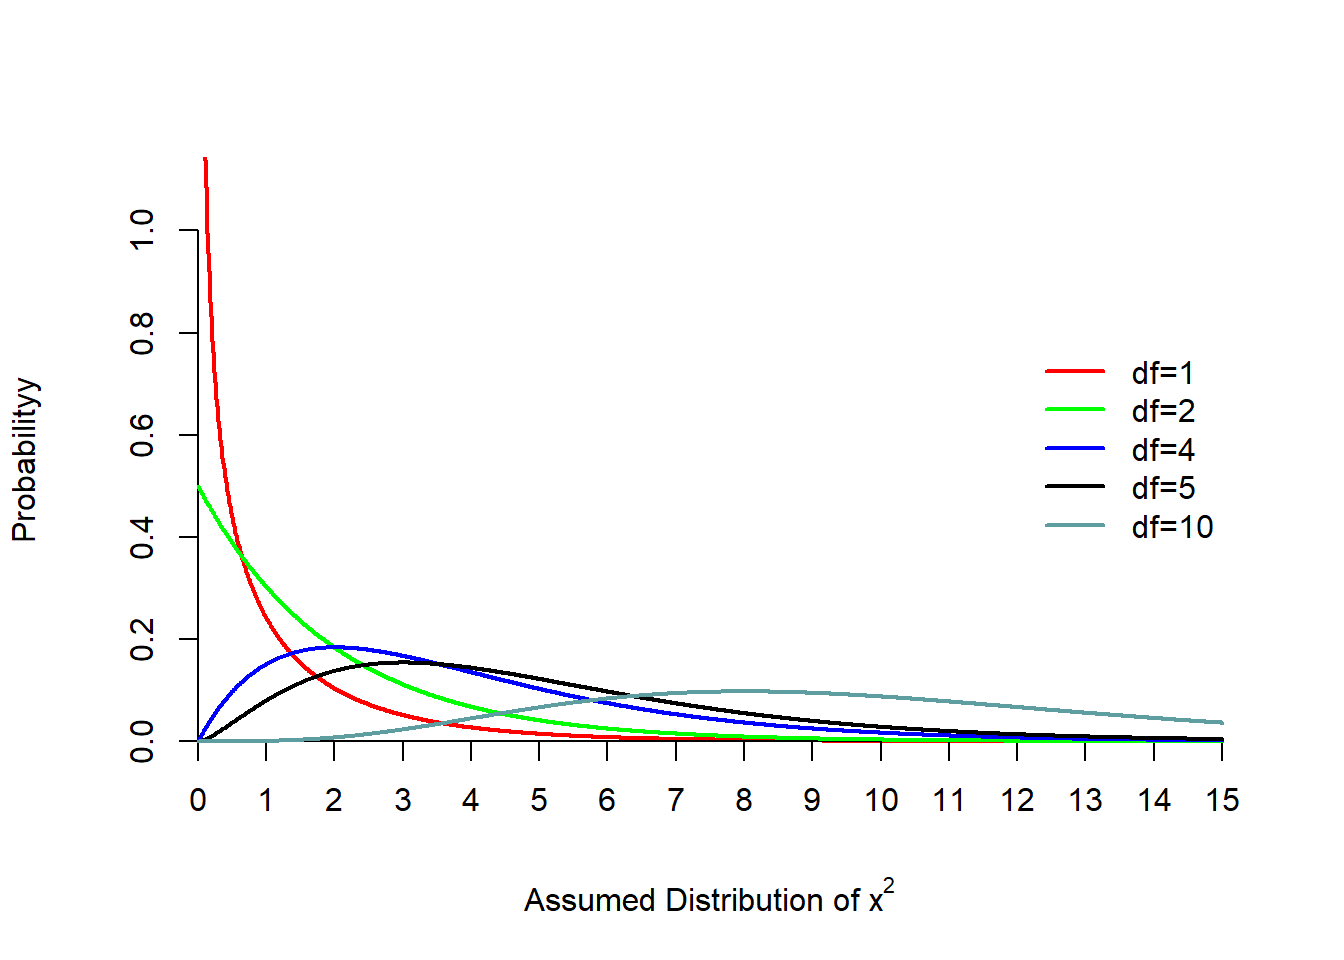
\includegraphics[width=0.55\linewidth]{figs/chisquaredfig} 

}

\caption{不同自由度情况下的卡方分布概率密度曲线图}\label{fig:chisquaredfig}
\end{figure}

\hypertarget{ux6982ux7387ux5bc6ux5ea6ux51fdux6570}{%
\subsubsection{概率密度函数}\label{ux6982ux7387ux5bc6ux5ea6ux51fdux6570}}

卡方分布的概率密度函数为:
\[f(x,v)=\frac{x^{v/2-1}e^{-x/2}}{2^{v/2}\Gamma(v/2)}\]
注意的是,当x≤0时,\(f(x,v)=0\);\(\Gamma\)代表Gamma函数,因此卡方分布也是一种特别的Gamma函数。

卡方分布的均值和方差分别为v,和2v,及自由度和自由度的2倍。

卡方分布的一个基本性质就是可加性,即独立卡方变量之和同样服从卡方分布。如两个独立的卡方分布,\(X_1 \sim X^2(v_1)\)与\(X_2 \sim X^2(v_2)\),那么有
\((X_1+X_2) \sim X^2(v_1+v_2)\)

在R语言中。卡方分布也有几个与Z分布,t分布基本函数类似的工具函数,分别是\href{https://www.rdocumentation.org/packages/stats/versions/3.6.2/topics/Chisquare}{dchisq(),pchisq(),qchisq()和rchisq()},
对应的检验函数主要是\href{https://www.rdocumentation.org/packages/stats/versions/3.6.2/topics/chisq.test}{chisq.test()}。

\hypertarget{ux5361ux65b9ux68c0ux9a8c}{%
\subsection{卡方检验}\label{ux5361ux65b9ux68c0ux9a8c}}

卡方检验(Chi-Squared Test)是一种统计量的分布在零假设成立时近似服从卡方分布的假设检验。在没有其他的限定条件或说明时,
卡方检验一般指代的是\textbf{皮尔森卡方检验}。在卡方检验的一般运用中,研究人员将观察量的值划分成若干互斥的分类,
且使用一套理论(或零假设)尝试去说明观察量的值落入不同分类的概率分布的模型。
而卡方检验的目的就在于去衡量这个假设对观察结果所反映的程度。卡方检验就是统计样本的实际观测值与理论推断值之间的偏离程度,
实际观测值与理论推断值之间的偏离程度就决定卡方值的大小,如果卡方值越大,二者偏差程度越大;
反之,二者偏差越小;若两个值完全相等时,卡方值就为0,表明理论值完全符合。

卡方检验分为\textbf{卡方独立性检验}和\textbf{拟合优度的卡方检验}。

\hypertarget{ux5361ux65b9ux72ecux7acbux6027ux68c0ux9a8cux7684ux57faux672cux601dux60f3}{%
\subsubsection{卡方独立性检验的基本思想}\label{ux5361ux65b9ux72ecux7acbux6027ux68c0ux9a8cux7684ux57faux672cux601dux60f3}}

这里使用《医学统计学》中的 案例07-01 的数据,介绍\(\chi^2\)检验的基本思想,详细见\protect\hyperlink{ux56dbux683cux8d44ux6599ux8868ux7684ux5361ux65b9ux68c0ux9a8c}{四格资料表的卡方检验}。

\hypertarget{ux56dbux683cux8d44ux6599ux8868ux7684ux5361ux65b9ux68c0ux9a8c}{%
\subsubsection{四格资料表的卡方检验}\label{ux56dbux683cux8d44ux6599ux8868ux7684ux5361ux65b9ux68c0ux9a8c}}

《医学统计学》中的 案例07-01 的数据,即四格资料表的比较为例,介绍\(\chi^2\)检验的基本思想。

\begin{table}

\caption{\label{tab:chisqtab}案例07-01 四格资料表}
\centering
\begin{tabular}[t]{ccccc}
\toprule
组别 & 有效 & 无效 & 合计 & 有效率\%\\
\midrule
试验组 & 99(90.48)a & 5(13.52)b & 104(a+b) & 95.20(a/(a+b))\\
对照组 & 75(83.52)c & 21(12.48)d & 96(c+d) & 78.13(c/(c+d)))\\
合计 & 174(a+c) & 26(b+d) & 200(n) & 87.00((a+c)/n)\\
\bottomrule
\end{tabular}
\end{table}

案例07-01 的四格资料表有a=99,b=5,c=75和d=21四个基本数据,其余数据都是根据它们计算出来的。现在想知道处理组与对照组两组样本代表总体有无差别,
即为两样本率比较的资料,既可以使用二项分布里面的\protect\hyperlink{ux4e24ux6837ux672cux7387ux7684ux6bd4ux8f83ux28ux6b63ux6001ux8fd1ux4f3cux29}{\textbf{u检验}},也可以利用卡方检验。
我们设计的原假设\(H_0:\) 处理组与对照组是来自同一总体,即\(P_{treatment}=P_{control}\)。

\textbf{u检验方法}

下面是用u检验的代码,根据计算结果,P值=0.0003362066\textless0.01\textless0.05,所以根据u检验结果,表明拒绝\(H_0\),接受备择假设\(H_1\),
即可以认为两种处理有显著性差异。

\begin{Shaded}
\begin{Highlighting}[]
\NormalTok{n5<-}\DecValTok{104}
\NormalTok{n6<-}\DecValTok{96}
\NormalTok{x5<-}\DecValTok{99}
\NormalTok{x6<-}\DecValTok{75}
\KeywordTok{binom_twosamplecomp_uAsym}\NormalTok{(n5,x5,n6,x6)}
\CommentTok{# [1] 0.0006442179}
\NormalTok{binom_twosamplecomp_uAsym<-}\ControlFlowTok{function}\NormalTok{(n1,x1,n2,x2)\{}
\NormalTok{     p1<-x1}\OperatorTok{/}\NormalTok{n1}
\NormalTok{     p2<-x2}\OperatorTok{/}\NormalTok{n2}
\NormalTok{     S_val<-}\KeywordTok{sqrt}\NormalTok{((x1}\OperatorTok{+}\NormalTok{x2)}\OperatorTok{/}\NormalTok{(n1}\OperatorTok{+}\NormalTok{n2)}\OperatorTok{*}\NormalTok{(}\DecValTok{1}\OperatorTok{-}\NormalTok{(x1}\OperatorTok{+}\NormalTok{x2)}\OperatorTok{/}\NormalTok{(n1}\OperatorTok{+}\NormalTok{n2))}\OperatorTok{*}\NormalTok{(}\DecValTok{1}\OperatorTok{/}\NormalTok{n1}\OperatorTok{+}\DecValTok{1}\OperatorTok{/}\NormalTok{n2))}
\NormalTok{     p_val<-}\KeywordTok{pnorm}\NormalTok{((p1}\OperatorTok{-}\NormalTok{p2)}\OperatorTok{/}\NormalTok{S_val,}\DataTypeTok{lower.tail =}\NormalTok{ F)}\OperatorTok{*}\DecValTok{2}
     \KeywordTok{return}\NormalTok{( p_val)}
\NormalTok{\}}

\end{Highlighting}
\end{Shaded}

\textbf{卡方检验方法}

卡方检验设计的原假设用u检验的一样,即\(H_0:\) 处理组与对照组是来自同一总体,\(P_{treatment}=P_{control}\)。

卡方检验的统计量计算的是\(\chi^2\),其计算公式和对应的卡方分布自由度计算方法为:
\[\chi^2=\sum{\frac{(A-T)^2}{T}} \\
v=(行数-1)(列数-1)\]
此公式也叫做皮尔森卡方检验(Pearson \(\chi^2\)),其中的A代表实际观察频数(Actual frequency),
即上面表格中的abcd四个值;T代表的\(H_0\)成立时的理论频数(Theoretical frequency),即假设处理组和对照组是来自同一总体,
且总体的有效率的P值根据观察值计算得到为\(p_0=174/200=87%
\)和\(q=1-p_0\),然后用p,q与处理组和对照组的样本数
分别计算有效,无效的理论频数,计算公式可以换算为:
\[T_{rc}=\frac{n_r*n_c}{n}\]
其中,\(T_{rc}\)为第r行第c列的理论频数,\(n_{r}\)和\(n_{c}\)分别是相应第r行的合计样本数,
和第c列的合计样本数;n为的行列的总样本数。

对于四格表资料的\(\chi^2\)检验的卡方值,也可以使用下面专用公式计算:
\[\chi^2=\frac{(ad-bc)^2n}{(a+b)(c+d)(a+c)(b+d)}\]

下面是采用卡方检验的代码,根据计算结果,P值=0.0003362066\textless0.01\textless0.05, 表明拒绝\(H_0\),接受备择假设\(H_1\),
即可以认为两种处理有显著性差异,同u检验的结论一致。

\begin{Shaded}
\begin{Highlighting}[]
\NormalTok{a<-}\DecValTok{99}
\NormalTok{b<-}\DecValTok{5}
\NormalTok{c<-}\DecValTok{75}
\NormalTok{d<-}\DecValTok{21}

\NormalTok{actual_matrix <-}\StringTok{ }\KeywordTok{matrix}\NormalTok{(}\DataTypeTok{data =} \KeywordTok{c}\NormalTok{(a,b,c,d), }\DataTypeTok{nrow =} \DecValTok{2}\NormalTok{, }\DataTypeTok{ncol =} \DecValTok{2}\NormalTok{,}\DataTypeTok{byrow =}\NormalTok{ T)}

\NormalTok{chisquare_fourfoldtable_test<-}\ControlFlowTok{function}\NormalTok{(actual_matrix)\{}
\NormalTok{     n<-}\KeywordTok{sum}\NormalTok{(actual_matrix)}
\NormalTok{     df<-(}\KeywordTok{dim}\NormalTok{(actual_matrix)[}\DecValTok{1}\NormalTok{]}\OperatorTok{-}\DecValTok{1}\NormalTok{)}\OperatorTok{*}\NormalTok{(}\KeywordTok{dim}\NormalTok{(actual_matrix)[}\DecValTok{2}\NormalTok{]}\OperatorTok{-}\DecValTok{1}\NormalTok{)}
\NormalTok{     chi_val<-}\DecValTok{0}
\NormalTok{     newmatrix<-}\KeywordTok{matrix}\NormalTok{(}\DataTypeTok{nrow =} \KeywordTok{dim}\NormalTok{(actual_matrix)[}\DecValTok{1}\NormalTok{],}\DataTypeTok{ncol =} \KeywordTok{dim}\NormalTok{(actual_matrix)[}\DecValTok{2}\NormalTok{])}
     \ControlFlowTok{for}\NormalTok{(i }\ControlFlowTok{in} \DecValTok{1}\OperatorTok{:}\KeywordTok{dim}\NormalTok{(actual_matrix)[}\DecValTok{1}\NormalTok{])\{}
          \ControlFlowTok{for}\NormalTok{(j }\ControlFlowTok{in} \DecValTok{1}\OperatorTok{:}\KeywordTok{dim}\NormalTok{(actual_matrix)[}\DecValTok{2}\NormalTok{])\{}
\NormalTok{          newmatrix[i,j]=(}\KeywordTok{sum}\NormalTok{(actual_matrix[i,])}\OperatorTok{*}\KeywordTok{sum}\NormalTok{(actual_matrix[,j]))}\OperatorTok{/}\NormalTok{n}
\NormalTok{          chi_val=chi_val}\OperatorTok{+}\NormalTok{(actual_matrix[i,j]}\OperatorTok{-}\NormalTok{newmatrix[i,j])}\OperatorTok{^}\DecValTok{2}\OperatorTok{/}\NormalTok{newmatrix[i,j]}
\NormalTok{          \}}
\NormalTok{     \}}
     \CommentTok{#print(chi_val)}
     \CommentTok{# [1] 12.85707}
\NormalTok{    p_val<-}\KeywordTok{pchisq}\NormalTok{(chi_val,df,,}\DataTypeTok{lower.tail =}\NormalTok{ F)}
     \KeywordTok{return}\NormalTok{ (p_val)}
\NormalTok{\}}
\KeywordTok{chisquare_fourfoldtable_test}\NormalTok{(actual_matrix)}
\CommentTok{# [1] 0.0003362066}

\CommentTok{###四格资料卡方检验的专用公式函数}
\NormalTok{chisquare_fourfoldtable_test1<-}\ControlFlowTok{function}\NormalTok{(actual_matrix)\{}
\NormalTok{     n<-}\KeywordTok{sum}\NormalTok{(actual_matrix)}
\NormalTok{     df<-(}\KeywordTok{dim}\NormalTok{(actual_matrix)[}\DecValTok{1}\NormalTok{]}\OperatorTok{-}\DecValTok{1}\NormalTok{)}\OperatorTok{*}\NormalTok{(}\KeywordTok{dim}\NormalTok{(actual_matrix)[}\DecValTok{2}\NormalTok{]}\OperatorTok{-}\DecValTok{1}\NormalTok{)}
\NormalTok{     chi_val<-(actual_matrix[}\DecValTok{1}\NormalTok{,}\DecValTok{1}\NormalTok{]}\OperatorTok{*}\NormalTok{actual_matrix[}\DecValTok{2}\NormalTok{,}\DecValTok{2}\NormalTok{]}\OperatorTok{-}\NormalTok{actual_matrix[}\DecValTok{1}\NormalTok{,}\DecValTok{2}\NormalTok{]}\OperatorTok{*}\NormalTok{actual_matrix[}\DecValTok{2}\NormalTok{,}\DecValTok{1}\NormalTok{])}\OperatorTok{^}\DecValTok{2}\OperatorTok{*}\NormalTok{n}\OperatorTok{/}\NormalTok{((actual_matrix[}\DecValTok{1}\NormalTok{,}\DecValTok{1}\NormalTok{]}\OperatorTok{+}\NormalTok{actual_matrix[}\DecValTok{1}\NormalTok{,}\DecValTok{2}\NormalTok{])}\OperatorTok{*}\NormalTok{(actual_matrix[}\DecValTok{2}\NormalTok{,}\DecValTok{1}\NormalTok{]}\OperatorTok{+}\NormalTok{actual_matrix[}\DecValTok{2}\NormalTok{,}\DecValTok{2}\NormalTok{])}\OperatorTok{*}\NormalTok{(actual_matrix[}\DecValTok{1}\NormalTok{,}\DecValTok{1}\NormalTok{]}\OperatorTok{+}\NormalTok{actual_matrix[}\DecValTok{2}\NormalTok{,}\DecValTok{1}\NormalTok{])}\OperatorTok{*}\NormalTok{(actual_matrix[}\DecValTok{1}\NormalTok{,}\DecValTok{2}\NormalTok{]}\OperatorTok{+}\NormalTok{actual_matrix[}\DecValTok{2}\NormalTok{,}\DecValTok{2}\NormalTok{]))}
     \CommentTok{#print(chi_val)}
     \CommentTok{# [1] 12.85707}
\NormalTok{     p_val<-}\KeywordTok{pchisq}\NormalTok{(chi_val,df,,}\DataTypeTok{lower.tail =}\NormalTok{ F)}
     \KeywordTok{return}\NormalTok{ (p_val)}
\NormalTok{\}}
\KeywordTok{chisquare_fourfoldtable_test1}\NormalTok{(actual_matrix)}

\CommentTok{##或者可以使用chisq.test()函数}
\NormalTok{chitest<-}\KeywordTok{chisq.test}\NormalTok{(actual_matrix,}\DataTypeTok{correct =}\NormalTok{ F)}
\NormalTok{chitest}\OperatorTok{$}\NormalTok{p.value}
\CommentTok{# [1] 0.0003362066}
\end{Highlighting}
\end{Shaded}

\hypertarget{ux56dbux683cux8d44ux6599ux8868ux7684ux5361ux65b9ux68c0ux9a8cux7684ux6821ux6b63ux516cux5f0f}{%
\paragraph{四格资料表的卡方检验的校正公式}\label{ux56dbux683cux8d44ux6599ux8868ux7684ux5361ux65b9ux68c0ux9a8cux7684ux6821ux6b63ux516cux5f0f}}

计数资料中的实际频数A为分类资料,是非连续的,由此使用卡方检验的统计量计算的\(\chi^2\)值也是非连续的,
当自由度v特别小,尤其是四格表这样只有1的时候,计算出的卡方值会偏小,导致p值偏大,导致第一类错误的概率增大。
为此,美国统计学家F. Yates在1934年提出了一个计算卡方值的连续性校正公式:
\[\chi^2=\sum\frac{(|A-T|-0.5)^2}{T}\]
或者修正后的专用公式计算为:
\[\chi^2=\frac{(|ad-bc|-n/2)^2n}{(a+b)(c+d)(a+c)(b+d)}\]

在实际工作中,对四格表资料使用卡方检验的规定是:

\begin{enumerate}
\def\labelenumi{\arabic{enumi}.}
\tightlist
\item
  当n≥40且T≥5时,用\(\chi^2\)检验的基本公式或专用公式计算;当P值≈α时,改用四格资料的卡方检验的\protect\hyperlink{Fisherux786eux5207ux6982ux7387ux6cd5}{Fisher确切概率法};
\item
  当n≥40且5\textgreater T≥1时,用\(\chi^2\)检验的校正公式或校正后的专用公式计算;或改用四格资料的卡方检验的\protect\hyperlink{Fisherux786eux5207ux6982ux7387ux6cd5}{Fisher确切概率法};
\item
  当n\textless40或1\textgreater T时,用卡方检验的\protect\hyperlink{Fisherux786eux5207ux6982ux7387ux6cd5}{Fisher确切概率法};
\end{enumerate}

使用《医学统计学》中的 案例07-02 的数据,即两样本率比较的\(\chi^2\)检验为例,

\begin{table}

\caption{\label{tab:chisqtab1}案例07-02 四格资料表}
\centering
\begin{tabular}[t]{ccccc}
\toprule
组别 & 有效 & 无效 & 合计 & 有效率\%\\
\midrule
胞磷胆碱组 & 46 & 18 & 64 & 88.46\\
神经节苷脂组 & 6 & 8 & 14 & 69.23\\
合计 & 52 & 26 & 78 & 82.05\\
\bottomrule
\end{tabular}
\end{table}

在R总的实现代码可以参考下面,采用了经典的计算方法和校正后的计算方法做对比。经典的计算结果显示\(\chi^2\)值为4.352679,
对应的P值为0.03695079\textless0.05;校正后的计算结果显示\(\chi^2\)值为3.1448,对应的P值为0.07616886\textgreater0.05,两者结果相反。

\begin{Shaded}
\begin{Highlighting}[]
\NormalTok{a<-}\DecValTok{46}
\NormalTok{b<-}\DecValTok{6}
\NormalTok{c<-}\DecValTok{18}
\NormalTok{d<-}\DecValTok{8}

\NormalTok{actual_matrix <-}\StringTok{ }\KeywordTok{matrix}\NormalTok{(}\DataTypeTok{data =} \KeywordTok{c}\NormalTok{(a,b,c,d), }\DataTypeTok{nrow =} \DecValTok{2}\NormalTok{, }\DataTypeTok{ncol =} \DecValTok{2}\NormalTok{,}\DataTypeTok{byrow =}\NormalTok{ T)}

\NormalTok{chisquare_fourfoldtable_test<-}\ControlFlowTok{function}\NormalTok{(actual_matrix)\{}
\NormalTok{     n<-}\KeywordTok{sum}\NormalTok{(actual_matrix)}
\NormalTok{     df<-(}\KeywordTok{dim}\NormalTok{(actual_matrix)[}\DecValTok{1}\NormalTok{]}\OperatorTok{-}\DecValTok{1}\NormalTok{)}\OperatorTok{*}\NormalTok{(}\KeywordTok{dim}\NormalTok{(actual_matrix)[}\DecValTok{2}\NormalTok{]}\OperatorTok{-}\DecValTok{1}\NormalTok{)}
\NormalTok{     chi_val<-}\DecValTok{0}
\NormalTok{     theoretical_matrix<-}\KeywordTok{matrix}\NormalTok{(}\DataTypeTok{nrow =} \KeywordTok{dim}\NormalTok{(actual_matrix)[}\DecValTok{1}\NormalTok{],}\DataTypeTok{ncol =} \KeywordTok{dim}\NormalTok{(actual_matrix)[}\DecValTok{2}\NormalTok{])}
     \ControlFlowTok{for}\NormalTok{(i }\ControlFlowTok{in} \DecValTok{1}\OperatorTok{:}\KeywordTok{dim}\NormalTok{(actual_matrix)[}\DecValTok{1}\NormalTok{])\{}
          \ControlFlowTok{for}\NormalTok{(j }\ControlFlowTok{in} \DecValTok{1}\OperatorTok{:}\KeywordTok{dim}\NormalTok{(actual_matrix)[}\DecValTok{2}\NormalTok{])\{}
\NormalTok{          theoretical_matrix[i,j]=(}\KeywordTok{sum}\NormalTok{(actual_matrix[i,])}\OperatorTok{*}\KeywordTok{sum}\NormalTok{(actual_matrix[,j]))}\OperatorTok{/}\NormalTok{n}
          \CommentTok{#chi_val=chi_val+(actual_matrix[i,j]-theoretical_matrix[i,j])^2/newmatrix[i,j]}
\NormalTok{          \}}
\NormalTok{     \}}
     \ControlFlowTok{if}\NormalTok{(}\KeywordTok{length}\NormalTok{(}\KeywordTok{which}\NormalTok{(theoretical_matrix}\OperatorTok{<}\DecValTok{1}\NormalTok{))}\OperatorTok{>=}\DecValTok{1} \OperatorTok{||}\StringTok{ }\NormalTok{n}\OperatorTok{<}\DecValTok{40}\NormalTok{)\{}
          \KeywordTok{print}\NormalTok{(}\StringTok{"Fisher 确切检验"}\NormalTok{)}
\NormalTok{          fisher_out<-}\KeywordTok{fisher.test}\NormalTok{(actual_matrix)}
          \KeywordTok{return}\NormalTok{(fisher_out}\OperatorTok{$}\NormalTok{p.value)}
\NormalTok{     \}}\ControlFlowTok{else} \ControlFlowTok{if}\NormalTok{(}\KeywordTok{length}\NormalTok{(}\KeywordTok{which}\NormalTok{(theoretical_matrix}\OperatorTok{<=}\DecValTok{5}\NormalTok{))}\OperatorTok{>=}\DecValTok{1} \OperatorTok{&&}\StringTok{ }\NormalTok{n}\OperatorTok{>=}\DecValTok{40}\NormalTok{)\{}
          \KeywordTok{print}\NormalTok{(}\StringTok{"校正后的卡方检验"}\NormalTok{)}
\NormalTok{          chi_val<-chi_val}\OperatorTok{+}\KeywordTok{chisquare_fourfoldtable_updated}\NormalTok{(actual_matrix,n)}
\NormalTok{     \}}\ControlFlowTok{else} \ControlFlowTok{if}\NormalTok{(}\KeywordTok{length}\NormalTok{(}\KeywordTok{which}\NormalTok{(theoretical_matrix}\OperatorTok{<}\DecValTok{5}\NormalTok{))}\OperatorTok{==}\DecValTok{0} \OperatorTok{&&}\StringTok{ }\NormalTok{n}\OperatorTok{>=}\DecValTok{40}\NormalTok{)\{}
          \KeywordTok{print}\NormalTok{(}\StringTok{"经典的卡方检验"}\NormalTok{)}
\NormalTok{          chi_val<-chi_val}\OperatorTok{+}\KeywordTok{chisquare_fourfoldtable_classical}\NormalTok{(actual_matrix,n)}
\NormalTok{     \}}
\NormalTok{     p_val<-}\KeywordTok{pchisq}\NormalTok{(chi_val,df,}\DataTypeTok{lower.tail=}\NormalTok{F)}
     \KeywordTok{cat}\NormalTok{(}\KeywordTok{paste}\NormalTok{(}\StringTok{"chi_val"}\NormalTok{,chi_val,}\StringTok{"}\CharTok{\textbackslash{}n}\StringTok{p_val"}\NormalTok{,p_val,}\DataTypeTok{sep=}\StringTok{"}\CharTok{\textbackslash{}t}\StringTok{"}\NormalTok{))}
     \KeywordTok{return}\NormalTok{ (p_val)}
\NormalTok{\}}

\NormalTok{chisquare_fourfoldtable_classical<-}\ControlFlowTok{function}\NormalTok{(actual_matrix,n)\{}
\NormalTok{     n<-}\KeywordTok{sum}\NormalTok{(actual_matrix)}
\NormalTok{     df<-(}\KeywordTok{dim}\NormalTok{(actual_matrix)[}\DecValTok{1}\NormalTok{]}\OperatorTok{-}\DecValTok{1}\NormalTok{)}\OperatorTok{*}\NormalTok{(}\KeywordTok{dim}\NormalTok{(actual_matrix)[}\DecValTok{2}\NormalTok{]}\OperatorTok{-}\DecValTok{1}\NormalTok{)}
\NormalTok{     chi_val<-(actual_matrix[}\DecValTok{1}\NormalTok{,}\DecValTok{1}\NormalTok{]}\OperatorTok{*}\NormalTok{actual_matrix[}\DecValTok{2}\NormalTok{,}\DecValTok{2}\NormalTok{]}\OperatorTok{-}\NormalTok{actual_matrix[}\DecValTok{1}\NormalTok{,}\DecValTok{2}\NormalTok{]}\OperatorTok{*}\NormalTok{actual_matrix[}\DecValTok{2}\NormalTok{,}\DecValTok{1}\NormalTok{])}\OperatorTok{^}\DecValTok{2}\OperatorTok{*}\NormalTok{n}\OperatorTok{/}\NormalTok{((actual_matrix[}\DecValTok{1}\NormalTok{,}\DecValTok{1}\NormalTok{]}\OperatorTok{+}\NormalTok{actual_matrix[}\DecValTok{1}\NormalTok{,}\DecValTok{2}\NormalTok{])}\OperatorTok{*}\NormalTok{(actual_matrix[}\DecValTok{2}\NormalTok{,}\DecValTok{1}\NormalTok{]}\OperatorTok{+}\NormalTok{actual_matrix[}\DecValTok{2}\NormalTok{,}\DecValTok{2}\NormalTok{])}\OperatorTok{*}\NormalTok{(actual_matrix[}\DecValTok{1}\NormalTok{,}\DecValTok{1}\NormalTok{]}\OperatorTok{+}\NormalTok{actual_matrix[}\DecValTok{2}\NormalTok{,}\DecValTok{1}\NormalTok{])}\OperatorTok{*}\NormalTok{(actual_matrix[}\DecValTok{1}\NormalTok{,}\DecValTok{2}\NormalTok{]}\OperatorTok{+}\NormalTok{actual_matrix[}\DecValTok{2}\NormalTok{,}\DecValTok{2}\NormalTok{]))}
     \CommentTok{#p_val<-dchisq(chi_val,df)}
     \KeywordTok{return}\NormalTok{ (chi_val)}
\NormalTok{\}}

\NormalTok{chisquare_fourfoldtable_updated<-}\ControlFlowTok{function}\NormalTok{(actual_matrix,n)\{}
\NormalTok{     n<-}\KeywordTok{sum}\NormalTok{(actual_matrix)}
\NormalTok{     df<-(}\KeywordTok{dim}\NormalTok{(actual_matrix)[}\DecValTok{1}\NormalTok{]}\OperatorTok{-}\DecValTok{1}\NormalTok{)}\OperatorTok{*}\NormalTok{(}\KeywordTok{dim}\NormalTok{(actual_matrix)[}\DecValTok{2}\NormalTok{]}\OperatorTok{-}\DecValTok{1}\NormalTok{)}
\NormalTok{     chi_val<-((}\KeywordTok{abs}\NormalTok{((actual_matrix[}\DecValTok{1}\NormalTok{,}\DecValTok{1}\NormalTok{]}\OperatorTok{*}\NormalTok{actual_matrix[}\DecValTok{2}\NormalTok{,}\DecValTok{2}\NormalTok{]}\OperatorTok{-}\NormalTok{actual_matrix[}\DecValTok{1}\NormalTok{,}\DecValTok{2}\NormalTok{]}\OperatorTok{*}\NormalTok{actual_matrix[}\DecValTok{2}\NormalTok{,}\DecValTok{1}\NormalTok{]))}\OperatorTok{-}\NormalTok{n}\OperatorTok{/}\DecValTok{2}\NormalTok{)}\OperatorTok{^}\DecValTok{2}\NormalTok{)}\OperatorTok{*}\NormalTok{n}\OperatorTok{/}
\StringTok{     }\NormalTok{((actual_matrix[}\DecValTok{1}\NormalTok{,}\DecValTok{1}\NormalTok{]}\OperatorTok{+}\NormalTok{actual_matrix[}\DecValTok{1}\NormalTok{,}\DecValTok{2}\NormalTok{])}\OperatorTok{*}\NormalTok{(actual_matrix[}\DecValTok{2}\NormalTok{,}\DecValTok{1}\NormalTok{]}\OperatorTok{+}\NormalTok{actual_matrix[}\DecValTok{2}\NormalTok{,}\DecValTok{2}\NormalTok{])}\OperatorTok{*}\NormalTok{(actual_matrix[}\DecValTok{1}\NormalTok{,}\DecValTok{1}\NormalTok{]}\OperatorTok{+}\NormalTok{actual_matrix[}\DecValTok{2}\NormalTok{,}\DecValTok{1}\NormalTok{])}\OperatorTok{*}\NormalTok{(actual_matrix[}\DecValTok{1}\NormalTok{,}\DecValTok{2}\NormalTok{]}\OperatorTok{+}\NormalTok{actual_matrix[}\DecValTok{2}\NormalTok{,}\DecValTok{2}\NormalTok{]))}
     \CommentTok{#p_val<-dchisq(chi_val,df)}
     \KeywordTok{return}\NormalTok{ (chi_val)}
\NormalTok{\}}

\CommentTok{##print("校正后的卡方检验")}
\KeywordTok{chisquare_fourfoldtable_test}\NormalTok{(actual_matrix)}
\CommentTok{# [1] 0.07616886}

\CommentTok{##print("经典的卡方检验")}
\KeywordTok{chisquare_fourfoldtable_classical}\NormalTok{(actual_matrix)}
\CommentTok{# [1] 4.352679}
\KeywordTok{pchisq}\NormalTok{(}\KeywordTok{chisquare_fourfoldtable_classical}\NormalTok{(actual_matrix),}\DecValTok{1}\NormalTok{,}\DataTypeTok{lower.tail =}\NormalTok{ F)}
\CommentTok{# [1] 0.03695079}
\end{Highlighting}
\end{Shaded}

\hypertarget{ux914dux5bf9ux7684ux56dbux683cux8d44ux6599ux8868ux7684ux5361ux65b9ux68c0ux9a8c}{%
\subsubsection{配对的四格资料表的卡方检验}\label{ux914dux5bf9ux7684ux56dbux683cux8d44ux6599ux8868ux7684ux5361ux65b9ux68c0ux9a8c}}

计数资料的配对设计常用于两种检验方法、培养方法、诊断方法的比较。其特点是对样本中各观察单位分别用两种方法处理,
然后观察两种处理方法的某两分类变量的计数结果。观察结果有四种情况:

\begin{enumerate}
\def\labelenumi{\arabic{enumi}.}
\tightlist
\item
  两种检测方法皆为阳性数(a);
\item
  两种检测方法皆为阴性数(d);
\item
  免疫荧光法为阳性,乳胶凝集法为阴性数(b);
\item
  乳胶凝集法为阳性,免疫荧光法为阴性数(c)。
\end{enumerate}

可整理成下表的形式,以《医学统计学》中的 案例07-07 的数据为例。

\begin{table}

\caption{\label{tab:chisqtab2}案例07-07 配对四格资料表}
\centering
\begin{tabular}[t]{cccc}
\toprule
\multicolumn{1}{c}{ } & \multicolumn{2}{c}{乳胶凝集法} & \multicolumn{1}{c}{ } \\
\cmidrule(l{3pt}r{3pt}){2-3}
免疫荧光法 & 阳性 & 阴性 & 合计\\
\midrule
阳性 & 11(a) & 2(c) & 13(a+c)\\
阴性 & 12(b) & 33(d) & 45(b+d)\\
合计 & 23(a+b) & 35(c+d) & 58(n)\\
\bottomrule
\end{tabular}
\end{table}

其中,a、d为两法观察结果一致的两种情况,b、c为两法观察结果不一致的两种情况。当两种处理方法无差别时,根据\href{https://www.statisticssolutions.com/mcnemar-marginal-homogeneity-sign-wilcoxon-tests/}{边际同质性}的零假设规定,
每个结果两个边缘概率是相同的,\(p_a + p_b = p_a + p_c\) 并且 \(p_c + p_d = p_b + p_d\),即两总体率相等\(p_b=p_c\),由于在抽样研究中,抽样误差是不可避免的,样本中的b和c往往不等
(b≠c,即两样本率不等:\(p_b=p_c\))。为此,需进行\href{https://en.wikipedia.org/wiki/McNemar\%27s_test}{麦克尼马尔假设检验(McNemar's test)},其检验统计量为:

\textbf{当 (b+c)≥40 时}:
\[\chi^2=\frac{(b-c)^2}{b+c}, v=1\]
\textbf{或者当 (b+c)\textless40 时}:
\[\chi^2=\frac{(|b-c|-1)^2}{b+c}, v=1\]
值得注意的时,麦克尼马尔假设检验一般用于样本含量不太大的资料,因为它只考虑了两种处理不一致的情况(b,c),
而没有考虑样本含量n和两种处理结果一致的情况(a,d),所以行n很大,且a,d的数值也很大时,b,c相对较小,
检验结果的实际意义就不明确了。

使用《医学统计学》中的 案例07-07 的数据,做麦克尼马尔假设检验的R实现。

\begin{Shaded}
\begin{Highlighting}[]
\NormalTok{a<-}\DecValTok{11}
\NormalTok{b<-}\DecValTok{12}
\NormalTok{c<-}\DecValTok{2}
\NormalTok{d<-}\DecValTok{33}
\NormalTok{actual_matrix <-}\StringTok{ }\KeywordTok{matrix}\NormalTok{(}\DataTypeTok{data =} \KeywordTok{c}\NormalTok{(a,b,c,d), }\DataTypeTok{nrow =} \DecValTok{2}\NormalTok{, }\DataTypeTok{ncol =} \DecValTok{2}\NormalTok{,}\DataTypeTok{byrow =}\NormalTok{ T)}

\NormalTok{chisquare_pairedfourfoldtable_test<-}\ControlFlowTok{function}\NormalTok{(actual_matrix)\{}
\NormalTok{     n<-}\KeywordTok{sum}\NormalTok{(actual_matrix)}
\NormalTok{     df<-(}\KeywordTok{dim}\NormalTok{(actual_matrix)[}\DecValTok{1}\NormalTok{]}\OperatorTok{-}\DecValTok{1}\NormalTok{)}\OperatorTok{*}\NormalTok{(}\KeywordTok{dim}\NormalTok{(actual_matrix)[}\DecValTok{2}\NormalTok{]}\OperatorTok{-}\DecValTok{1}\NormalTok{)}
     \CommentTok{#chi_val<-0}
\NormalTok{     un_same<-actual_matrix[}\DecValTok{1}\NormalTok{,}\DecValTok{2}\NormalTok{]}\OperatorTok{+}\NormalTok{actual_matrix[}\DecValTok{2}\NormalTok{,}\DecValTok{1}\NormalTok{]}
     \ControlFlowTok{if}\NormalTok{(un_same }\OperatorTok{>=}\StringTok{ }\DecValTok{40}\NormalTok{)\{}
          \KeywordTok{print}\NormalTok{(}\StringTok{"chisquare_pairedfourfoldtable_classical"}\NormalTok{)}
\NormalTok{          chi_val<-}\KeywordTok{chisquare_pairedfourfoldtable_classical}\NormalTok{(actual_matrix,n)}
\NormalTok{     \}}\ControlFlowTok{else} \ControlFlowTok{if}\NormalTok{(un_same }\OperatorTok{<}\StringTok{ }\DecValTok{40}\NormalTok{)\{}
          \KeywordTok{print}\NormalTok{(}\StringTok{"chisquare_fourfoldtable_updated"}\NormalTok{)}
\NormalTok{          chi_val<-}\KeywordTok{chisquare_pairedfourfoldtable_updated}\NormalTok{(actual_matrix,n)}
\NormalTok{     \}}
\NormalTok{     p_val<-}\KeywordTok{pchisq}\NormalTok{(chi_val,df,}\DataTypeTok{lower.tail=}\NormalTok{F)}
     \CommentTok{#cat(paste("chi_val",chi_val,"\textbackslash{}n p_val ",p_val,sep="\textbackslash{}t"))}
     \KeywordTok{return}\NormalTok{ (p_val)}
\NormalTok{\}}

\NormalTok{chisquare_pairedfourfoldtable_classical<-}\ControlFlowTok{function}\NormalTok{(actual_matrix,n)\{}
\NormalTok{     n<-}\KeywordTok{sum}\NormalTok{(actual_matrix)}
\NormalTok{     df<-(}\KeywordTok{dim}\NormalTok{(actual_matrix)[}\DecValTok{1}\NormalTok{]}\OperatorTok{-}\DecValTok{1}\NormalTok{)}\OperatorTok{*}\NormalTok{(}\KeywordTok{dim}\NormalTok{(actual_matrix)[}\DecValTok{2}\NormalTok{]}\OperatorTok{-}\DecValTok{1}\NormalTok{)}
\NormalTok{     chi_val<-(actual_matrix[}\DecValTok{1}\NormalTok{,}\DecValTok{2}\NormalTok{]}\OperatorTok{-}\NormalTok{actual_matrix[}\DecValTok{2}\NormalTok{,}\DecValTok{1}\NormalTok{])}\OperatorTok{^}\DecValTok{2}\OperatorTok{/}\NormalTok{(actual_matrix[}\DecValTok{1}\NormalTok{,}\DecValTok{2}\NormalTok{]}\OperatorTok{+}\NormalTok{actual_matrix[}\DecValTok{2}\NormalTok{,}\DecValTok{1}\NormalTok{])}
     \CommentTok{#p_val<-dchisq(chi_val,df)}
     \KeywordTok{return}\NormalTok{ (chi_val)}
\NormalTok{\}}

\NormalTok{chisquare_pairedfourfoldtable_updated<-}\ControlFlowTok{function}\NormalTok{(actual_matrix,n)\{}
\NormalTok{     n<-}\KeywordTok{sum}\NormalTok{(actual_matrix)}
\NormalTok{     df<-(}\KeywordTok{dim}\NormalTok{(actual_matrix)[}\DecValTok{1}\NormalTok{]}\OperatorTok{-}\DecValTok{1}\NormalTok{)}\OperatorTok{*}\NormalTok{(}\KeywordTok{dim}\NormalTok{(actual_matrix)[}\DecValTok{2}\NormalTok{]}\OperatorTok{-}\DecValTok{1}\NormalTok{)}
\NormalTok{     chi_val<-((}\KeywordTok{abs}\NormalTok{(actual_matrix[}\DecValTok{1}\NormalTok{,}\DecValTok{2}\NormalTok{]}\OperatorTok{-}\NormalTok{actual_matrix[}\DecValTok{2}\NormalTok{,}\DecValTok{1}\NormalTok{])}\OperatorTok{-}\DecValTok{1}\NormalTok{)}\OperatorTok{^}\DecValTok{2}\NormalTok{)}\OperatorTok{/}\NormalTok{(actual_matrix[}\DecValTok{1}\NormalTok{,}\DecValTok{2}\NormalTok{]}\OperatorTok{+}\NormalTok{actual_matrix[}\DecValTok{2}\NormalTok{,}\DecValTok{1}\NormalTok{])}
          \CommentTok{#p_val<-dchisq(chi_val,df)}
     \KeywordTok{return}\NormalTok{ (chi_val)}
\NormalTok{\}}
\KeywordTok{chisquare_pairedfourfoldtable_test}\NormalTok{(actual_matrix)}
\CommentTok{#[1] 0.01615693}

\CommentTok{#或者使用函数mcnemar.test()}
\KeywordTok{mcnemar.test}\NormalTok{(actual_matrix)}
\CommentTok{##      McNemar's Chi-squared test with continuity correction}
\CommentTok{##  }
\CommentTok{##  data:  actual_matrix}
\CommentTok{##  McNemar's chi-squared = 5.7857, df = 1, p-value = 0.01616}
\end{Highlighting}
\end{Shaded}

根据计算结果,P值=0.01615693\textless0.05,按α=0.05的检验水准,拒绝\(H_0\),接受\(H_1\),
即可认为两种方法的检验效率不一样。

\hypertarget{ux56dbux683cux8d44ux6599ux8868ux7684fisherux786eux5207ux6982ux7387ux6cd5}{%
\subsubsection{四格资料表的Fisher确切概率法}\label{ux56dbux683cux8d44ux6599ux8868ux7684fisherux786eux5207ux6982ux7387ux6cd5}}

四格表的Fisher确切概率法,即\href{https://en.wikipedia.org/wiki/Fisher\%27s_exact_test}{Fisher精确检验(Fisher's exact test)}又称四格表概率的直接计算,
常用于四格表资料的假设检验的补充,即通常对四格表中出现n\textless40或T\textless1,或用经典计算卡方值后的 P值≈α的情况,需改用Fisher确切概率法计算。
其基本思想是: 在四格表的\textbf{周边合计}不变的条件下,直接计算表内四个实际频数(a,b,c,d)的所有组合的概率\(P_i\),并且有\(\sum{P_i}\)=1。
各组合的概率服从\href{https://zh.wikipedia.org/zh-hans/\%E8\%B6\%85\%E5\%87\%A0\%E4\%BD\%95\%E5\%88\%86\%E5\%B8\%83}{超几何分布},
按检验假设取单侧或双侧的\textbf{累计概率P},即可按所取检验水准作出推断结论。

使用《医学统计学》中的 案例07-04 的数据,做四格表的Fisher确切概率法的R实现。

\begin{table}

\caption{\label{tab:chisqtab3}案例07-04 Fisher确切概率法四格资料表}
\centering
\begin{tabular}[t]{ccccc}
\toprule
组别 & 阳性 & 阴性 & 合计 & 感染率(\%)\\
\midrule
预防注射组 & 4 | a & 18 | b & 22 | a+b & 18.18\\
非预防组 & 5 | c & 6 | d & 11 | c+d & 45.45\\
合计 & 9 | a+c & 24 | b+d & 33 | n & 27.27\\
\bottomrule
\end{tabular}
\end{table}

\textbf{第一步:计算实际频数(a,b,c,d)的所有组合的概率\(P_i\)}

在四格表的周边合计不变的条件下,实际频数(a,b,c,d)的所有组合的的可能性共有``周边合计最小数+1''个,如案例07-04的实际频数
组合情况有min(a+c,a+b,c+d,b+d)+1=9+1=10种,详细见下图:

\begin{figure}

{\centering 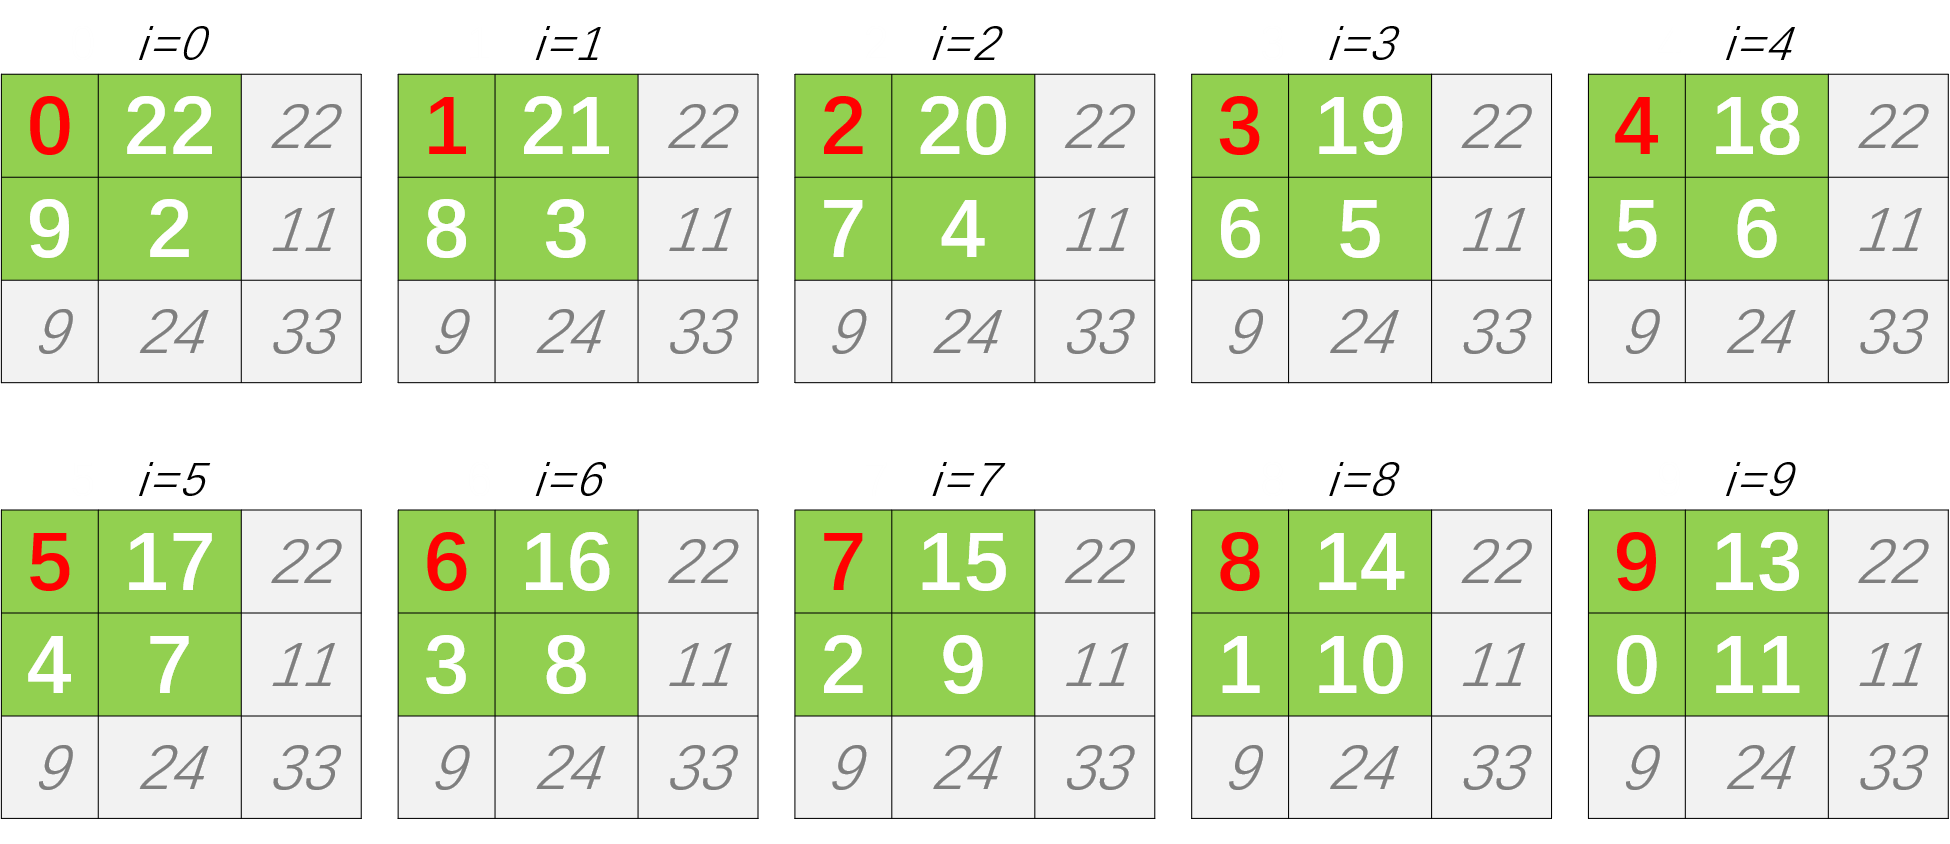
\includegraphics[width=0.7\linewidth]{image/Fisherchitest} 

}

\caption{案例 07-04的实际频数组合情况}\label{fig:Fisherchitest}
\end{figure}

各组合的概率\(P_i\)服从超几何分布,\(P_i\)的计算公式为:
\[P_i=\frac{(a+c)!(a+b)!(c+d)!(b+d)!}{a!b!c!d!n!}\]

\textbf{第二步:计算累积概率的P值}

一般的规定,\(P_i\)(i=1,2,3,\ldots)对应a从小到大的概率,那么各种组合下累计概率的计算,分单、双侧检验两种情况:

\begin{enumerate}
\def\labelenumi{\arabic{enumi}.}
\tightlist
\item
  单侧检验:现有样本的实际观察频率(记作\(P_a\))的左侧为左侧概率(记作\(P_l\)),备择假设\(H_1\)为 \(p_1 > p_2\);
  现有样本的实际观察频率(记作\(P_a\))的右侧为右侧概率(记作\(P_r\)),备择假设\(H_1\)为 \(p_1 < p_2\);
\item
  双侧检验: 若遇到a+b=c+d或a+c=b+d时,四格表各组序列呈对称分布,此时只计算\(P_i≤P_a\)的单侧概率,然后乘以2即算的双侧的累积概率值。
\end{enumerate}

注意的是,Fisher精确检验依赖的时\href{https://zh.wikipedia.org/zh-hans/\%E8\%B6\%85\%E5\%87\%A0\%E4\%BD\%95\%E5\%88\%86\%E5\%B8\%83}{超几何分布(Hypergeometric distribution)},
R语言中与超几何分布相关的主要函数有\href{https://stat.ethz.ch/R-manual/R-devel/library/stats/html/Hypergeometric.html}{dhyper(),phyper(),qhyper()和rhyper()}。

\begin{center}\rule{0.5\linewidth}{0.5pt}\end{center}

超几何分布:从一个有限的总体中进行不放回抽样,设其中包含有n个黑球(阳性/成功),m个白球(阴性/失败),若从中不放回地随机抽取k个(\(k\in[0,m+n]\)),
其中含有的不白球的个数为x(x=1,2,3,\ldots,k),则X的个数对应的概率即是服从超几何分布,记为X\textasciitilde h(k, n, m)。
案例07-04的数据可以视作:从一个总体为33的数据中进行不放回抽样,设其中包含有24个黑球(阳性/成功),9个白球(阴性/失败),若从中不放回地随机抽取22个(\(k\in[0,m+n]\)),
其中含有的白球的个数为x=1:9(m=9 \textless{} k=22),则X的个数对应的概率即是服从超几何分布,记为X\textasciitilde h(22, 24, 9)。

\begin{center}\rule{0.5\linewidth}{0.5pt}\end{center}

假设预防组和非预防组的来自同一总体,即\(H_0:p_1=p_2=9/33\),\(H_1:p_1≠p_2\),
同二项分布的应用中类似,主要是回答``有无差别'',及备择假设是\(p≠p_0\)是否成立,因此计算的是实际样本``成功''x次(实际频数,A=a)出现的概率,
与更背离原假设的事件出现的概率和。

\begin{Shaded}
\begin{Highlighting}[]
\NormalTok{a<-}\DecValTok{4}\NormalTok{;b<-}\DecValTok{18}\NormalTok{;}
\NormalTok{c<-}\DecValTok{5}\NormalTok{;d<-}\DecValTok{6}\NormalTok{;}
\NormalTok{actual_matrix <-}\StringTok{ }\KeywordTok{matrix}\NormalTok{(}\DataTypeTok{data =} \KeywordTok{c}\NormalTok{(a,b,c,d), }\DataTypeTok{nrow =} \DecValTok{2}\NormalTok{, }\DataTypeTok{ncol =} \DecValTok{2}\NormalTok{,}\DataTypeTok{byrow =}\NormalTok{ T)}

\NormalTok{m<-a}\OperatorTok{+}\NormalTok{c;n<-b}\OperatorTok{+}\NormalTok{d;k<-a}\OperatorTok{+}\NormalTok{b;}

\CommentTok{##使用dhyper()计算不同x值得p值}
\KeywordTok{dhyper}\NormalTok{(}\DataTypeTok{x=}\DecValTok{0}\OperatorTok{:}\DecValTok{9}\NormalTok{, }\DataTypeTok{m=}\NormalTok{m, }\DataTypeTok{n=}\NormalTok{n, }\DataTypeTok{k=}\NormalTok{k)}
\KeywordTok{dhyper}\NormalTok{(}\DataTypeTok{x=}\NormalTok{a, }\DataTypeTok{m=}\NormalTok{m, }\DataTypeTok{n=}\NormalTok{n, }\DataTypeTok{k=}\NormalTok{k)}
\CommentTok{#0.08762728}

\CommentTok{#计算出现4次各情况的累计概率值}
\NormalTok{p4<-}\KeywordTok{dhyper}\NormalTok{(}\DataTypeTok{x=}\NormalTok{a, }\DataTypeTok{m=}\NormalTok{m, }\DataTypeTok{n=}\NormalTok{n, }\DataTypeTok{k=}\NormalTok{k)}
\CommentTok{#0.08762728}
\CommentTok{#计算出现更背离原假设的事件及概率,即:}
\NormalTok{p4_}\DecValTok{1}\NormalTok{<-}\KeywordTok{sum}\NormalTok{(}\KeywordTok{dhyper}\NormalTok{(}\DecValTok{0}\OperatorTok{:}\NormalTok{m, }\DataTypeTok{m=}\NormalTok{m, }\DataTypeTok{n=}\NormalTok{n, }\DataTypeTok{k=}\NormalTok{k)[}\KeywordTok{which}\NormalTok{(}\KeywordTok{dhyper}\NormalTok{(}\DecValTok{0}\OperatorTok{:}\NormalTok{m, }\DataTypeTok{m=}\NormalTok{m, }\DataTypeTok{n=}\NormalTok{n, }\DataTypeTok{k=}\NormalTok{k)}\OperatorTok{<}\KeywordTok{dhyper}\NormalTok{(}\DataTypeTok{x=}\NormalTok{a, }\DataTypeTok{m=}\NormalTok{m, }\DataTypeTok{n=}\NormalTok{n, }\DataTypeTok{k=}\NormalTok{k))])}
\CommentTok{# [1] 0.03341747}
\CommentTok{#双侧检验的p值为:}
\NormalTok{p4}\OperatorTok{+}\NormalTok{p4_}\DecValTok{1}
\CommentTok{# [1] 0.1210448}

\CommentTok{#或者直接用which()函数一并计算}
\KeywordTok{sum}\NormalTok{(}\KeywordTok{dhyper}\NormalTok{(}\DecValTok{0}\OperatorTok{:}\NormalTok{m, }\DataTypeTok{m=}\NormalTok{m, }\DataTypeTok{n=}\NormalTok{n, }\DataTypeTok{k=}\NormalTok{k)[}\KeywordTok{which}\NormalTok{(}\KeywordTok{dhyper}\NormalTok{(}\DecValTok{0}\OperatorTok{:}\NormalTok{m, }\DataTypeTok{m=}\NormalTok{m, }\DataTypeTok{n=}\NormalTok{n, }\DataTypeTok{k=}\NormalTok{k)}\OperatorTok{<=}\KeywordTok{dhyper}\NormalTok{(}\DataTypeTok{x=}\NormalTok{a, }\DataTypeTok{m=}\NormalTok{m, }\DataTypeTok{n=}\NormalTok{n, }\DataTypeTok{k=}\NormalTok{k))])}
\CommentTok{# [1] 0.1210448}

\CommentTok{#或者使用fisher.test()}
\KeywordTok{fisher.test}\NormalTok{(actual_matrix,}\DataTypeTok{alternative =} \StringTok{"two.sided"}\NormalTok{)}
\CommentTok{##      Fisher's Exact Test for Count Data}
\CommentTok{##  }
\CommentTok{##  data:  actual_matrix}
\CommentTok{##  p-value = 0.121}
\CommentTok{##  alternative hypothesis: true odds ratio is not equal to 1}
\CommentTok{##  95 percent confidence interval:}
\CommentTok{##   0.03974151 1.76726409}
\CommentTok{##  sample estimates:}
\CommentTok{##  odds ratio }
\CommentTok{##   0.2791061 }
\end{Highlighting}
\end{Shaded}

根据计算结果,p值=0.1210448\textgreater0.05,不拒绝\(H_0: p_1=p_1\),即还不能认为两种处理得感染率不同。

使用《医学统计学》中的 案例07-05 的数据,做四格表的Fisher确切概率法的R实现。

\begin{Shaded}
\begin{Highlighting}[]
\NormalTok{a<-}\DecValTok{6}\NormalTok{;b<-}\DecValTok{4}\NormalTok{;}
\NormalTok{c<-}\DecValTok{1}\NormalTok{;d<-}\DecValTok{9}\NormalTok{;}
\NormalTok{actual_matrix <-}\StringTok{ }\KeywordTok{matrix}\NormalTok{(}\DataTypeTok{data =} \KeywordTok{c}\NormalTok{(a,b,c,d), }\DataTypeTok{nrow =} \DecValTok{2}\NormalTok{, }\DataTypeTok{ncol =} \DecValTok{2}\NormalTok{,}\DataTypeTok{byrow =}\NormalTok{ T)}

\NormalTok{m<-a}\OperatorTok{+}\NormalTok{c;n<-b}\OperatorTok{+}\NormalTok{d;k<-a}\OperatorTok{+}\NormalTok{b;}
\KeywordTok{sum}\NormalTok{(}\KeywordTok{dhyper}\NormalTok{(}\DecValTok{0}\OperatorTok{:}\NormalTok{m, }\DataTypeTok{m=}\NormalTok{m, }\DataTypeTok{n=}\NormalTok{n, }\DataTypeTok{k=}\NormalTok{k)[}\KeywordTok{which}\NormalTok{(}\KeywordTok{dhyper}\NormalTok{(}\DecValTok{0}\OperatorTok{:}\NormalTok{m, }\DataTypeTok{m=}\NormalTok{m, }\DataTypeTok{n=}\NormalTok{n, }\DataTypeTok{k=}\NormalTok{k)}\OperatorTok{<=}\KeywordTok{dhyper}\NormalTok{(}\DataTypeTok{x=}\NormalTok{a, }\DataTypeTok{m=}\NormalTok{m, }\DataTypeTok{n=}\NormalTok{n, }\DataTypeTok{k=}\NormalTok{k))])}
\CommentTok{# [1] 0.05727554}

\CommentTok{#或者使用fisher.test()}
\KeywordTok{fisher.test}\NormalTok{(actual_matrix,}\DataTypeTok{alternative =} \StringTok{"two.sided"}\NormalTok{)}
\CommentTok{##      Fisher's Exact Test for Count Data}
\CommentTok{##  }
\CommentTok{##  data:  actual_matrix}
\CommentTok{##  p-value = 0.05728}
\CommentTok{##  alternative hypothesis: true odds ratio is not equal to 1}
\CommentTok{##  95 percent confidence interval:}
\CommentTok{##     0.9487882 684.4235629}
\CommentTok{##  sample estimates:}
\CommentTok{##  odds ratio }
\CommentTok{##     11.6367 }
\end{Highlighting}
\end{Shaded}

根据计算结果,p值=0.05727554\textgreater0.05,不拒绝\(H_0: p_1=p_1\),记即还不能认为两种肿瘤中\(P_{53}\)基因的表达率不同。

注意的是,如果专业上有理由肿瘤A中的\(P_{53}\)基因的表达率高于肿瘤B中,那么这里应该进行单侧检验,\(H_1: p_1>p_2\),
计算P值应该是\(P_r\),反之可以计算\(P_l\)。

\hypertarget{ux884cux5217ux8d44ux6599ux8868ux7684ux5361ux65b9ux68c0ux9a8c}{%
\subsection{行列资料表的卡方检验}\label{ux884cux5217ux8d44ux6599ux8868ux7684ux5361ux65b9ux68c0ux9a8c}}

行x列表资料的卡方检验用于多个样本率的比较、两个或多个构成比的比较以及双向无序分类资料的 关联性检验。
其基本数据有以下3种情况:

\begin{enumerate}
\def\labelenumi{\arabic{enumi}.}
\item
  多个样本率比较时,有R行2列,称为Rx2表;
\item
  两个样本 的构成比比较时,有2行C列,称2xC表;
\item
  多个样本的构成比比较以及双向无序分类资料关联性检验时,有R行C列,称为RxC表。
\end{enumerate}

以上3种情况可统称为行×列表资料。行x列表资料的检验仍用 Pearsony \(\chi^2\)公式 计算检验统计量值。
因该式需先计算理论频数 \(T_{rc}\),化简后得行×列表资料检验的专用公式和自由度为:
\[\chi^2=n(\sum\frac{A^2}{n_{r}n_{c}}-1),v=(行数-1)(列数-1)\]

其中的A代表实际观察频数(Actual frequency),n\_\{r\}\(和\)n\_\{c\}\$分别是相应第r行的合计样本数和第c列的合计样本数。

\hypertarget{ux591aux4e2aux6837ux672cux7387ux7684ux6bd4ux8f83r-times-2ux8868}{%
\subsubsection{\texorpdfstring{多个样本率的比较(\(R \times 2\)表)}{多个样本率的比较(R \textbackslash times 2表)}}\label{ux591aux4e2aux6837ux672cux7387ux7684ux6bd4ux8f83r-times-2ux8868}}

使用《医学统计学》中的 案例07-06 的数据,做多个样本率的比较的卡方检验和R实现。

\begin{table}

\caption{\label{tab:chisqtab4}案例07-06 3x2 表资料的多个样本率的比较测试数据}
\centering
\begin{tabular}[t]{ccccc}
\toprule
疗法 & 有效 & 无效 & 合计 & 有效率(\%)\\
\midrule
物理疗法组 & 199 & 7 & 206 & 96.60\\
药物疗法组 & 164 & 18 & 182 & 90.11\\
外用膏药组 & 118 & 26 & 144 & 81.94\\
合计 & 481 & 51 & 532 & 90.41\\
\bottomrule
\end{tabular}
\end{table}

设置的原假设\(H_0: p_1=p_2=p_3\),即三种疗法的治疗的有效率是一样的;相应的备择假设\$H\_1:\$3种治疗方法的有效率不都一样。

\begin{Shaded}
\begin{Highlighting}[]
\NormalTok{actual_matrix <-}\StringTok{ }\KeywordTok{matrix}\NormalTok{(}\DataTypeTok{data =} \KeywordTok{as.numeric}\NormalTok{( }\KeywordTok{c}\NormalTok{(}\StringTok{"199"}\NormalTok{,}\StringTok{"164"}\NormalTok{,}\StringTok{"118"}\NormalTok{,}\StringTok{"7"}\NormalTok{,}\StringTok{"18"}\NormalTok{,}\StringTok{"26"}\NormalTok{)), }
\DataTypeTok{nrow =} \DecValTok{3}\NormalTok{, }\DataTypeTok{ncol =} \DecValTok{2}\NormalTok{,}\DataTypeTok{byrow =}\NormalTok{ F)}

\NormalTok{chisquare_rctable_multiratio_test<-}\ControlFlowTok{function}\NormalTok{(actual_matrix)\{}
\NormalTok{     n=}\KeywordTok{sum}\NormalTok{(actual_matrix)}
\NormalTok{     df<-(}\KeywordTok{dim}\NormalTok{(actual_matrix)[}\DecValTok{1}\NormalTok{]}\OperatorTok{-}\DecValTok{1}\NormalTok{)}\OperatorTok{*}\NormalTok{(}\KeywordTok{dim}\NormalTok{(actual_matrix)[}\DecValTok{2}\NormalTok{]}\OperatorTok{-}\DecValTok{1}\NormalTok{)}
\NormalTok{     chi_val<-n}\OperatorTok{*}\NormalTok{(}\OperatorTok{-}\DecValTok{1}\NormalTok{)}
     \ControlFlowTok{for}\NormalTok{(i }\ControlFlowTok{in} \DecValTok{1}\OperatorTok{:}\KeywordTok{dim}\NormalTok{(actual_matrix)[}\DecValTok{1}\NormalTok{])\{}
          \ControlFlowTok{for}\NormalTok{(j }\ControlFlowTok{in} \DecValTok{1}\OperatorTok{:}\KeywordTok{dim}\NormalTok{(actual_matrix)[}\DecValTok{2}\NormalTok{])\{}
\NormalTok{               chi_val<-chi_val}\OperatorTok{+}\NormalTok{n}\OperatorTok{*}\NormalTok{(actual_matrix[i,j]}\OperatorTok{^}\DecValTok{2}\OperatorTok{/}\NormalTok{(}\KeywordTok{sum}\NormalTok{(actual_matrix[i,])}\OperatorTok{*}\KeywordTok{sum}\NormalTok{(actual_matrix[,j])))}
\NormalTok{          \}}
\NormalTok{     \}}
     \CommentTok{#cat("chi_val: ",chi_val)}
\NormalTok{     p_val<-}\KeywordTok{pchisq}\NormalTok{(chi_val,df,}\DataTypeTok{lower.tail=}\NormalTok{F)}\OperatorTok{*}\DecValTok{2} 
     \KeywordTok{return}\NormalTok{(p_val)}
\NormalTok{\}}
\KeywordTok{chisquare_rctable_multiratio_test}\NormalTok{(actual_matrix)}
\CommentTok{# [1] 5.404583e-05}
\end{Highlighting}
\end{Shaded}

根据计算结果,p值=5.404583e-05\textless0.001\textless0.01\textless0.05,即拒绝原假设\(H_0\),接受\(H_1\),认为三种治疗方法的有效率不都一样。
注意,这里同方差分析类似,我们后面还会进一步讨论这种情况的多组比较,即探讨三种疗法具体谁比较好,谁比较差。

\hypertarget{ux6837ux672cux6784ux6210ux6bd4ux7684ux6bd4ux8f832-times-cux8868}{%
\subsubsection{\texorpdfstring{样本构成比的比较(\(2 \times C\)表)}{样本构成比的比较(2 \textbackslash times C表)}}\label{ux6837ux672cux6784ux6210ux6bd4ux7684ux6bd4ux8f832-times-cux8868}}

\begin{table}

\caption{\label{tab:chisqtab5}案例07-07 2x3 表资料的多个样本率的比较测试数据}
\centering
\begin{tabular}[t]{ccccc}
\toprule
组别 & DD & ID & II & 合计\\
\midrule
DN组 & 42 & 48 & 21 & 111\\
无DN组 & 30 & 72 & 36 & 138\\
合计 & 72 & 120 & 57 & 249\\
\bottomrule
\end{tabular}
\end{table}

设置的原假设\(H_0:\) 即在某疾病的两组亚型涉及的基因A的基因型的总体构成比是一样的;相应的备择假设\(H_1:\)某疾病的两组亚型涉及的基因A的基因型的总体构成比不都一样。

\begin{Shaded}
\begin{Highlighting}[]
\NormalTok{actual_matrix <-}\StringTok{ }\KeywordTok{matrix}\NormalTok{(}\DataTypeTok{data =} \KeywordTok{as.numeric}\NormalTok{( }\KeywordTok{c}\NormalTok{(}\StringTok{"42"}\NormalTok{,}\StringTok{"30"}\NormalTok{,}\StringTok{"48"}\NormalTok{,}\StringTok{"72"}\NormalTok{,}\StringTok{"21"}\NormalTok{,}\StringTok{"36"}\NormalTok{)), }
\DataTypeTok{nrow =} \DecValTok{2}\NormalTok{, }\DataTypeTok{ncol =} \DecValTok{3}\NormalTok{,}\DataTypeTok{byrow =}\NormalTok{ F)}

\NormalTok{chisquare_rctable_multiratio_test<-}\ControlFlowTok{function}\NormalTok{(actual_matrix)\{}
\NormalTok{     n=}\KeywordTok{sum}\NormalTok{(actual_matrix)}
\NormalTok{     df<-(}\KeywordTok{dim}\NormalTok{(actual_matrix)[}\DecValTok{1}\NormalTok{]}\OperatorTok{-}\DecValTok{1}\NormalTok{)}\OperatorTok{*}\NormalTok{(}\KeywordTok{dim}\NormalTok{(actual_matrix)[}\DecValTok{2}\NormalTok{]}\OperatorTok{-}\DecValTok{1}\NormalTok{)}
\NormalTok{     chi_val<-n}\OperatorTok{*}\NormalTok{(}\OperatorTok{-}\DecValTok{1}\NormalTok{)}
     \ControlFlowTok{for}\NormalTok{(i }\ControlFlowTok{in} \DecValTok{1}\OperatorTok{:}\KeywordTok{dim}\NormalTok{(actual_matrix)[}\DecValTok{1}\NormalTok{])\{}
          \ControlFlowTok{for}\NormalTok{(j }\ControlFlowTok{in} \DecValTok{1}\OperatorTok{:}\KeywordTok{dim}\NormalTok{(actual_matrix)[}\DecValTok{2}\NormalTok{])\{}
\NormalTok{               chi_val<-chi_val}\OperatorTok{+}\NormalTok{n}\OperatorTok{*}\NormalTok{(actual_matrix[i,j]}\OperatorTok{^}\DecValTok{2}\OperatorTok{/}\NormalTok{(}\KeywordTok{sum}\NormalTok{(actual_matrix[i,])}\OperatorTok{*}\KeywordTok{sum}\NormalTok{(actual_matrix[,j])))}
\NormalTok{          \}}
\NormalTok{     \}}
     \CommentTok{#cat("chi_val: ",chi_val)}
\NormalTok{     p_val<-}\KeywordTok{pchisq}\NormalTok{(chi_val,df,}\DataTypeTok{lower.tail=}\NormalTok{F)}\OperatorTok{*}\DecValTok{2} 
     \KeywordTok{return}\NormalTok{(p_val)}
\NormalTok{\}}
\KeywordTok{chisquare_rctable_multiratio_test}\NormalTok{(actual_matrix)}
\CommentTok{# [1] 0.01913288}
\end{Highlighting}
\end{Shaded}

根据计算结果,p值=0.01913288\textless0.05,即拒绝原假设\(H_0\),接受\(H_1\),认为两组亚型涉及的基因A的基因型的
总体构成比不都一样。

\hypertarget{ux53ccux5411ux65e0ux5e8fux5206ux7ec4ux8d44ux6599ux7684ux5173ux8054ux6027ux68c0ux9a8c}{%
\subsubsection{双向无序分组资料的关联性检验}\label{ux53ccux5411ux65e0ux5e8fux5206ux7ec4ux8d44ux6599ux7684ux5173ux8054ux6027ux68c0ux9a8c}}

对于两个分类变量皆为 \textbf{无序分类变量} 的行x列表资料料,又称为双向无序RxC表资料。若是一个样本的双向无序
RxC表资料,常常分析两个分类变量之间有无关系?关系的密切程度如何? 此时可用行x列表资料\(\chi^2\)检验来推断两
个分类变量之间有无关系(或关联); 在有关系的前提下,若须进一步分析关系的密切程度时,可计算 Pearson 列联系数C,
其计算公式为:
\[C=\sqrt{\frac{\chi^2}{n+\chi^2}}\]

式中\(\chi^2\)为行×列表资料的\(\chi^2\)值,n为样本含量。列联系数C取值范围在0\textasciitilde1之间,愈接近于0,关系愈不密切;愈接近于1,关系愈密切。

\begin{table}

\caption{\label{tab:chisqtab6}案例07-08 rxc 表资料的双向无序分组资料的关联性检验测试数据}
\centering
\begin{tabular}[t]{ccccc}
\toprule
\multicolumn{1}{c}{ } & \multicolumn{3}{c}{MN血型} & \multicolumn{1}{c}{ } \\
\cmidrule(l{3pt}r{3pt}){2-4}
ABO血型 & M & N & MN & 合计\\
\midrule
O & 431 & 490 & 902 & 1823\\
A & 388 & 410 & 800 & 1598\\
B & 495 & 587 & 950 & 2032\\
AB & 137 & 179 & 32 & 348\\
合计 & 1451 & 1666 & 2684 & 5801\\
\bottomrule
\end{tabular}
\end{table}

设置的原假设\(H_0:\) 两种血型系统之间没有关联;相应的备择假设\(H_1:\)两种血型系统之间有关联。

\begin{Shaded}
\begin{Highlighting}[]

\NormalTok{actual_matrix <-}\StringTok{ }\KeywordTok{matrix}\NormalTok{(}\DataTypeTok{data =} \KeywordTok{as.numeric}\NormalTok{( }\KeywordTok{c}\NormalTok{(}\StringTok{"431"}\NormalTok{,}\StringTok{"388"}\NormalTok{,}\StringTok{"495"}\NormalTok{,}\StringTok{"137"}\NormalTok{,}\StringTok{"490"}\NormalTok{,}\StringTok{"410"}\NormalTok{,}\StringTok{"587"}\NormalTok{,}\StringTok{"179"}\NormalTok{,}\StringTok{"902"}\NormalTok{,}\StringTok{"800"}\NormalTok{,}\StringTok{"950"}\NormalTok{,}\StringTok{"32"}\NormalTok{)), }
\DataTypeTok{nrow =} \DecValTok{4}\NormalTok{, }\DataTypeTok{ncol =} \DecValTok{3}\NormalTok{,}\DataTypeTok{byrow =}\NormalTok{ F)}

\NormalTok{chisquare_rctable_multiratio_test<-}\ControlFlowTok{function}\NormalTok{(actual_matrix)\{}
\NormalTok{     n=}\KeywordTok{sum}\NormalTok{(actual_matrix)}
\NormalTok{     df<-(}\KeywordTok{dim}\NormalTok{(actual_matrix)[}\DecValTok{1}\NormalTok{]}\OperatorTok{-}\DecValTok{1}\NormalTok{)}\OperatorTok{*}\NormalTok{(}\KeywordTok{dim}\NormalTok{(actual_matrix)[}\DecValTok{2}\NormalTok{]}\OperatorTok{-}\DecValTok{1}\NormalTok{)}
\NormalTok{     chi_val<-}\KeywordTok{chisquare_chivaler}\NormalTok{(actual_matrix)}
     \KeywordTok{cat}\NormalTok{(}\StringTok{"chi_val: "}\NormalTok{,chi_val,}\StringTok{"}\CharTok{\textbackslash{}n}\StringTok{ df: "}\NormalTok{,df)}
\NormalTok{     p_val<-}\KeywordTok{pchisq}\NormalTok{(chi_val,df,}\DataTypeTok{lower.tail=}\NormalTok{F)}\OperatorTok{*}\DecValTok{2} 
     \KeywordTok{return}\NormalTok{(p_val)}
\NormalTok{\}}

\NormalTok{chisquare_rctable_pearsonC<-}\ControlFlowTok{function}\NormalTok{(actual_matrix)\{}
\NormalTok{     n=}\KeywordTok{sum}\NormalTok{(actual_matrix)}
\NormalTok{     chi_val<-}\KeywordTok{chisquare_chivaler}\NormalTok{(actual_matrix)}
\NormalTok{     pearsonC<-}\KeywordTok{sqrt}\NormalTok{(chi_val}\OperatorTok{/}\NormalTok{(n}\OperatorTok{+}\NormalTok{chi_val))}
     \KeywordTok{return}\NormalTok{(pearsonC)}
\NormalTok{\}}

\NormalTok{chisquare_chivaler<-}\ControlFlowTok{function}\NormalTok{(actual_matrix)\{}
\NormalTok{     n=}\KeywordTok{sum}\NormalTok{(actual_matrix)}
\NormalTok{     chi_val<-n}\OperatorTok{*}\NormalTok{(}\OperatorTok{-}\DecValTok{1}\NormalTok{)}
     \ControlFlowTok{for}\NormalTok{(i }\ControlFlowTok{in} \DecValTok{1}\OperatorTok{:}\KeywordTok{dim}\NormalTok{(actual_matrix)[}\DecValTok{1}\NormalTok{])\{}
          \ControlFlowTok{for}\NormalTok{(j }\ControlFlowTok{in} \DecValTok{1}\OperatorTok{:}\KeywordTok{dim}\NormalTok{(actual_matrix)[}\DecValTok{2}\NormalTok{])\{}
\NormalTok{               chi_val<-chi_val}\OperatorTok{+}\NormalTok{n}\OperatorTok{*}\NormalTok{(actual_matrix[i,j]}\OperatorTok{^}\DecValTok{2}\OperatorTok{/}\NormalTok{(}\KeywordTok{sum}\NormalTok{(actual_matrix[i,])}\OperatorTok{*}\KeywordTok{sum}\NormalTok{(actual_matrix[,j])))}
\NormalTok{          \}}
\NormalTok{     \}}
     \KeywordTok{return}\NormalTok{(chi_val)}
\NormalTok{\}}

\KeywordTok{chisquare_rctable_multiratio_test}\NormalTok{(actual_matrix)}
\CommentTok{# [1] 5.971112e-43}
\KeywordTok{chisquare_rctable_pearsonC}\NormalTok{(actual_matrix)}
\CommentTok{# [1] 0.1882638}

\CommentTok{##或者可以用chisq.test()计算,但是p值函数使用的最小p值有关,}
\CommentTok{##默认情况返回的P值与上面的计算不一致}
\KeywordTok{chisq.test}\NormalTok{(actual_matrix)}
\CommentTok{##      Pearson's Chi-squared test}
\CommentTok{##  }
\CommentTok{##  data:  actual_matrix}
\CommentTok{##  X-squared = 213.16, df = 6, p-value < 2.2e-16}

\CommentTok{##列联系数也可以用DescTools包中的ContCoef()计算}
\NormalTok{DescTools}\OperatorTok{::}\KeywordTok{ContCoef}\NormalTok{(actual_matrix)}
\CommentTok{# [1] 0.1882638}
\end{Highlighting}
\end{Shaded}

根据计算结果,p值=5.971112e-43\textless0.01\textless0.05,因此拒绝原假设\(H_0\)。接受\(H_1\),即认为两种血型系统之间有关联。
其关联程度按照列联系数C=0.1882638,数值较小,虽然有统计学意义,但是关系不大,关于统计显著与专业意义的关系
可以\protect\hyperlink{ux53c2ux6570ux4f30ux8ba1ux4e0eux5047ux8bbeux68c0ux9a8cux7684ux8054ux7cfb}{参考参数估计与假设检验}的联系的内容。

\begin{center}\rule{0.5\linewidth}{0.5pt}\end{center}

分类变量可分为无序变量和有序变量两大类:

\begin{enumerate}
\def\labelenumi{\arabic{enumi}.}
\tightlist
\item
  无序分类变量,指所分类别zhi或属性之间无程度和dao顺序的差别。无序分类又可分为:

  \begin{itemize}
  \tightlist
  \item
    二项分类,如性别(男、女),药物反应(阴性,阳性)等;
  \item
    多项分类,如血型(O、A、B、AB),职业(工、农、商、学、兵)等。
    对于无序分类变量的分析,应先按类别分组,清点各组的观察单位数,编制分类变量的频数表,所得资料为无序分类资料,
    亦称计数资料。
  \end{itemize}
\item
  有序分类变量,指各类别之间有程度的差别。
  如尿糖化验结果按-、±、+、++、+++分类;疗效按治愈、显效、好转、无效分类。
  对于有序分类变量,应先按等级顺序分组,清点各组的观察单位个数,编制有序变量的频数表,所得资料称为等级资料。
\end{enumerate}

\begin{center}\rule{0.5\linewidth}{0.5pt}\end{center}

\hypertarget{ux53ccux5411ux6709ux5e8fux5206ux7ec4ux8d44ux6599ux7684ux7ebfux6027ux8d8bux52bfux68c0ux9a8c}{%
\subsubsection{双向有序分组资料的线性趋势检验}\label{ux53ccux5411ux6709ux5e8fux5206ux7ec4ux8d44ux6599ux7684ux7ebfux6027ux8d8bux52bfux68c0ux9a8c}}

对双向有序属性不同的RxC表资料,除可推断两个分类变量是否存在相关关系外,还可通过分解推断其相关是否为线性相关。
其基本思想是:首先计算RxC表资料的值,然后将总的值分解成\emph{线性回归分量}与\emph{偏离线性回归分量}。若两分量均有统计学意义,
说明两个分类变量存在相关关系,但关系不是简单的直线关系;若线性回归分量有统计学意义,偏离线性回归分量无统计学意义时,
说明两个分类变量存在直线相关关系。

计算过程如大致下:
1. 按照先前介绍的 行×列表资料检验的专用公式 \(\chi_{tol}^2=n(\sum\frac{A^2}{n_{r}n_{c}}-1)\)计算中的\(\chi^2\)值,自由度为\(v_{tol}=(行数-1)\times(列数-1)\)。
2. 计算线性回归分量\(\chi_{reg}^2\) 先给两个有序变量分别赋值(如X变量有-,+,++,其对应赋值1,2,3,···;Y变量有治愈、显效、好转、无效+对应赋值1,2,3,4···),再计算线性回归的\(\chi_{reg}^2\)恒量:
\[\chi_{reg}^2=\frac{b^2}{S_b^2}, v_{reg}=1,v_{reg}=1\]
其中b为回归系数,\(S_b^2\)为b的方差,\(b=l_{xy}/l_{xx}\),\(S_b^2=l_{yy}/(n*l_{xx})\),\(l_{xx},l_{yy}\)分别是
变量X,Y的离差平方和;\(l_{xy}\)是变量X,Y的离均差积和,f为样本观察频率即:
\[l_{xx}=\sum fx^2-\frac{(\sum fx)^2}{\sum f}\]
\[l_{yy}=\sum fy^2-\frac{(\sum fy)^2}{\sum f}\]
\[l_{xy}=\sum f(xy)-\frac{(\sum fx)(\sum fy)}{\sum f}\]
3. 计算偏离线性回归分量\(\chi_{wide}^2\),公式为:
\[\chi_{wide}^2=\chi_{tol}^2-\chi_{reg}^2,v_{wide}=v_{tol}-v_{reg}\]

使用《医学统计学》中的 案例07-09 的数据,做双向有序分组资料的线性趋势检验的R实现。

\begin{table}

\caption{\label{tab:chisqtab7}案例07-09 rxc 双向有序分组资料的线性趋势检验测试数据}
\centering
\begin{tabular}[t]{cccccc}
\toprule
\multicolumn{1}{c}{ } & \multicolumn{4}{c}{冠状动脉硬化等级(Y)} & \multicolumn{1}{c}{ } \\
\cmidrule(l{3pt}r{3pt}){2-5}
年龄(岁)X & \textbackslash{}- & \textbackslash{}+ & ++ & +++ & 合计\\
\midrule
20\textasciitilde{} & 70 & 22 & 4 & 2 & 98\\
30\textasciitilde{} & 27 & 24 & 9 & 3 & 62\\
40\textasciitilde{} & 16 & 23 & 13 & 7 & 59\\
≤50 & 9 & 20 & 15 & 14 & 58\\
合计 & 122 & 89 & 41 & 26 & 278\\
\bottomrule
\end{tabular}
\end{table}

设置的原假设\(H_0:\) 年龄与动脉硬化等级之间没有线性关系;相应的备择假设\(H_1:\)年龄与动脉硬化等级之间有线性关系。

\begin{Shaded}
\begin{Highlighting}[]
\NormalTok{actual_matrix <-}\StringTok{ }\KeywordTok{matrix}\NormalTok{(}\DataTypeTok{data =} \KeywordTok{as.numeric}\NormalTok{( }\KeywordTok{c}\NormalTok{(}\StringTok{"70"}\NormalTok{,}\StringTok{"27"}\NormalTok{,}\StringTok{"16"}\NormalTok{,}\StringTok{"9"}\NormalTok{,}\StringTok{"22"}\NormalTok{,}\StringTok{"24"}\NormalTok{,}\StringTok{"23"}\NormalTok{,}\StringTok{"20"}\NormalTok{,}\StringTok{"4"}\NormalTok{,}\StringTok{"9"}\NormalTok{,}\StringTok{"13"}\NormalTok{,}\StringTok{"15"}\NormalTok{,}\StringTok{"2"}\NormalTok{,}\StringTok{"3"}\NormalTok{,}\StringTok{"7"}\NormalTok{,}\StringTok{"14"}\NormalTok{)), }
\DataTypeTok{nrow =} \DecValTok{4}\NormalTok{, }\DataTypeTok{ncol =} \DecValTok{4}\NormalTok{,}\DataTypeTok{byrow =}\NormalTok{ F)}

\CommentTok{#计算总的卡方}
\NormalTok{chisquare_chivaler<-}\ControlFlowTok{function}\NormalTok{(actual_matrix)\{}
\NormalTok{     n=}\KeywordTok{sum}\NormalTok{(actual_matrix)}
\NormalTok{     chi_val<-n}\OperatorTok{*}\NormalTok{(}\OperatorTok{-}\DecValTok{1}\NormalTok{)}
     \ControlFlowTok{for}\NormalTok{(i }\ControlFlowTok{in} \DecValTok{1}\OperatorTok{:}\KeywordTok{dim}\NormalTok{(actual_matrix)[}\DecValTok{1}\NormalTok{])\{}
          \ControlFlowTok{for}\NormalTok{(j }\ControlFlowTok{in} \DecValTok{1}\OperatorTok{:}\KeywordTok{dim}\NormalTok{(actual_matrix)[}\DecValTok{2}\NormalTok{])\{}
\NormalTok{               chi_val<-chi_val}\OperatorTok{+}\NormalTok{n}\OperatorTok{*}\NormalTok{(actual_matrix[i,j]}\OperatorTok{^}\DecValTok{2}\OperatorTok{/}\NormalTok{(}\KeywordTok{sum}\NormalTok{(actual_matrix[i,])}\OperatorTok{*}\KeywordTok{sum}\NormalTok{(actual_matrix[,j])))}
\NormalTok{          \}}
\NormalTok{     \}}
     \KeywordTok{return}\NormalTok{(chi_val)}
\NormalTok{\}}

\CommentTok{#计算线性回归分量对应的卡方}
\NormalTok{chisquare_chivaler_4reg<-}\ControlFlowTok{function}\NormalTok{(actual_matrix)\{}
\NormalTok{     n=}\KeywordTok{sum}\NormalTok{(actual_matrix)}
\NormalTok{     actual_matrix_squ<-actual_matrix}\OperatorTok{^}\DecValTok{2}
\NormalTok{     fsum=n}
\NormalTok{     fXsum<-}\KeywordTok{sum}\NormalTok{(}\KeywordTok{apply}\NormalTok{(actual_matrix, }\DecValTok{1}\NormalTok{, sum)}\OperatorTok{*}\NormalTok{(}\DecValTok{1}\OperatorTok{:}\KeywordTok{dim}\NormalTok{(actual_matrix)[}\DecValTok{1}\NormalTok{]))}
\NormalTok{     fXXsum<-}\KeywordTok{sum}\NormalTok{(}\KeywordTok{apply}\NormalTok{(actual_matrix, }\DecValTok{1}\NormalTok{, sum)}\OperatorTok{*}\NormalTok{(}\DecValTok{1}\OperatorTok{:}\KeywordTok{dim}\NormalTok{(actual_matrix)[}\DecValTok{1}\NormalTok{])}\OperatorTok{^}\DecValTok{2}\NormalTok{)}
\NormalTok{     fYsum<-}\KeywordTok{sum}\NormalTok{(}\KeywordTok{apply}\NormalTok{(actual_matrix, }\DecValTok{2}\NormalTok{, sum)}\OperatorTok{*}\NormalTok{(}\DecValTok{1}\OperatorTok{:}\KeywordTok{dim}\NormalTok{(actual_matrix)[}\DecValTok{2}\NormalTok{]))}
\NormalTok{     fYYsum<-}\KeywordTok{sum}\NormalTok{(}\KeywordTok{apply}\NormalTok{(actual_matrix, }\DecValTok{2}\NormalTok{, sum)}\OperatorTok{*}\NormalTok{(}\DecValTok{1}\OperatorTok{:}\KeywordTok{dim}\NormalTok{(actual_matrix)[}\DecValTok{2}\NormalTok{])}\OperatorTok{^}\DecValTok{2}\NormalTok{)}
\NormalTok{     fXYsum<-}\DecValTok{0}
     \ControlFlowTok{for}\NormalTok{(x }\ControlFlowTok{in} \DecValTok{1}\OperatorTok{:}\KeywordTok{dim}\NormalTok{(actual_matrix)[}\DecValTok{1}\NormalTok{])\{}
          \ControlFlowTok{for}\NormalTok{(y }\ControlFlowTok{in} \DecValTok{1}\OperatorTok{:}\KeywordTok{dim}\NormalTok{(actual_matrix)[}\DecValTok{2}\NormalTok{])\{}
\NormalTok{               fXYsum<-fXYsum}\OperatorTok{+}\NormalTok{actual_matrix[x,y]}\OperatorTok{*}\NormalTok{x}\OperatorTok{*}\NormalTok{y}
\NormalTok{          \}}
\NormalTok{     \}}
     \CommentTok{#cat("fsum=",fsum,"fXsum=",fXsum,"fXXsum=",fXXsum,"fYsum=",fYsum,"fYYsum=",fYYsum,"fXYsum=",fXYsum)}
\NormalTok{     l_xx<-fXXsum}\OperatorTok{-}\NormalTok{fXsum}\OperatorTok{^}\DecValTok{2}\OperatorTok{/}\NormalTok{fsum}
\NormalTok{     l_yy<-fYYsum}\OperatorTok{-}\NormalTok{fYsum}\OperatorTok{^}\DecValTok{2}\OperatorTok{/}\NormalTok{fsum}
\NormalTok{     l_xy<-fXYsum}\OperatorTok{-}\NormalTok{fXsum}\OperatorTok{*}\NormalTok{fYsum}\OperatorTok{/}\NormalTok{fsum}
\NormalTok{     b<-l_xy}\OperatorTok{/}\NormalTok{l_xx}
\NormalTok{     SS_b<-l_yy}\OperatorTok{/}\NormalTok{(l_xx}\OperatorTok{*}\NormalTok{fsum)}
\NormalTok{     chi_val<-b}\OperatorTok{^}\DecValTok{2}\OperatorTok{/}\NormalTok{SS_b}
     \CommentTok{#cat("b=",b,"SS_b=",SS_b)}
     \KeywordTok{return}\NormalTok{(chi_val)}
\NormalTok{\}}

\NormalTok{chi_tol<-}\KeywordTok{chisquare_chivaler}\NormalTok{(actual_matrix)}
\CommentTok{# [1] 71.43249}
\NormalTok{chi_reg<-}\KeywordTok{chisquare_chivaler_4reg}\NormalTok{(actual_matrix)}
\CommentTok{# [1] 63.61832}
\NormalTok{chi_wide<-chi_tol}\OperatorTok{-}\NormalTok{chi_reg}
\CommentTok{# [1] 7.814174}
\KeywordTok{pchisq}\NormalTok{(chi_tol,(}\DecValTok{4-1}\NormalTok{)}\OperatorTok{*}\NormalTok{(}\DecValTok{4-1}\NormalTok{),}\DataTypeTok{lower.tail=}\NormalTok{F)}
\CommentTok{# [1] 7.969604e-12}
\KeywordTok{pchisq}\NormalTok{(chi_reg,}\DecValTok{1}\NormalTok{,}\DataTypeTok{lower.tail=}\NormalTok{F)}
\CommentTok{# [1] 1.510182e-15}
\KeywordTok{pchisq}\NormalTok{(chi_wide,(}\DecValTok{4-1}\NormalTok{)}\OperatorTok{*}\NormalTok{(}\DecValTok{4-1}\NormalTok{)}\OperatorTok{-}\DecValTok{1}\NormalTok{,}\DataTypeTok{lower.tail=}\NormalTok{F)}
\CommentTok{# [1] 0.4518296}

\CommentTok{##或者可以用chisq.test()计算总的卡方和p值}
\KeywordTok{chisq.test}\NormalTok{(actual_matrix)}
\end{Highlighting}
\end{Shaded}

\begin{table}

\caption{\label{tab:chisqtab8}双向有序分组资料的线性趋势检验测试结果}
\centering
\begin{tabular}[t]{cccc}
\toprule
变异来源 & \$\textbackslash{}chi\textasciicircum{}2\$ & 自由度 & P值\\
\midrule
总变异 & 71.43249 & 9 & 7.969604e-12\\
线性回归分量 & 63.61832 & 1 & 1.510182e-15\\
偏离线性回归分量 & 7.814174 & 8 & 0.4518296\\
\bottomrule
\end{tabular}
\end{table}

根据计算结果,线性回归分量的卡方P值=1.510182e-15\textless0.005\textless0.05,具有统计学意义;偏离线性回归分量的卡方P值=0.4518296\textgreater0.05,pchisq
不具有同继续意义,因此可以认为年龄与冠状动脉硬化之间存在线性相关的关系,结合资料表说明时随年龄增加动脉硬化风险升高。

\hypertarget{ux5361ux65b9ux68c0ux9a8cux7684ux6ce8ux610fux4e8bux9879ux4e0eux9009ux62e9ux601dux8def}{%
\subsubsection{卡方检验的注意事项与选择思路}\label{ux5361ux65b9ux68c0ux9a8cux7684ux6ce8ux610fux4e8bux9879ux4e0eux9009ux62e9ux601dux8def}}

\hypertarget{ux6ce8ux610fux4e8bux9879}{%
\paragraph{注意事项}\label{ux6ce8ux610fux4e8bux9879}}

\begin{enumerate}
\def\labelenumi{\arabic{enumi}.}
\item
  一般认为,行×列表资料中各格的理论频数不应小于1,并且1\textless7\textless5的格子数不宜超过格子总数 的1/5。若出现上述情况,可通过以下方法尝试解决:

  \begin{itemize}
  \tightlist
  \item
    最好是增加样本含量,使理论频数增大;
  \item
    根据专业知识,考虑能否删去理论频数太小的行或列,能否将理论频数太小的行或列与性质相近的邻行或邻列合并;
  \item
    改用双向无序R×C表资料的 Fisher 确切概率法。
  \end{itemize}
\item
  多个样本率比较,若所得统计推断为拒绝日,接受\(H_0\)时,只能认为各总休率之间总的来说有差別,
  但不能说明任两个总体率之间均有差别。要进一步推断哪两两总体字之间有差别,需进一步做\protect\hyperlink{ux591aux4e2aux6837ux672cux7387ux7684ux591aux91cdux6bd4ux8f83}{多个样本率的多重比较}。
\item
  医学期刊中常见这样的情况:不管RxC表资料中的两个分类变量是有序还是无序,均用\(\chi^2\)检验分析。这种做法是不妥的。对于有序的R×C表资料不宜用\(\chi^2\)检验,
  因为行×列表资料的\(\chi^2\)检验与分类变量的顺序无关,当有序变量的R×C表资料中的分类顺序固定不变时,无论将任何两行(或两列)频数互换,所得值皆不变,
  其结论相同,这显然是不妥的。因此在实际应用中,对于RxC表资料要根据其分类类型和研究目的选用恰当的检验方法。
\end{enumerate}

\hypertarget{ux9009ux62e9ux601dux8def}{%
\paragraph{选择思路}\label{ux9009ux62e9ux601dux8def}}

RxC表资料可以分为双向无序、单向有序、双向有序属性相同和双向有序属性不同4类。

\begin{enumerate}
\def\labelenumi{\arabic{enumi}.}
\item
  双向无序RxC表资料
  RxC表资料中两个分类变量皆为无序分类变量。对于该类资料,

  \begin{itemize}
  \tightlist
  \item
    若研究目的为多个样本率(或构成比)的比较,可用\protect\hyperlink{ux591aux4e2aux6837ux672cux7387ux7684ux6bd4ux8f83}{RxC表资料的\(\chi^2\)检验};
  \item
    若研究目的为分析两个分类变量之间有无关联性以及关系的密切程度时,可用RxC表资料的\(\chi^2\)检验以及\protect\hyperlink{ux53ccux5411ux65e0ux5e8fux5206ux7ec4ux8d44ux6599ux7684ux5173ux8054ux6027ux68c0ux9a8c}{Pearson 列联系数进行分析}。
  \end{itemize}
\item
  单向有序RxC表资料
  对于该类资料,有两种形式,

  \begin{itemize}
  \tightlist
  \item
    若RxC表资料中的分组变量(如年龄)是有序的,而指标变量(如传染病的类型)是无序的。其研究目的通常是分析不同年龄组各种传染病的构成情况,
    此种\protect\hyperlink{ux884cux5217ux8d44ux6599ux8868ux7684ux5361ux65b9ux68c0ux9a8c}{单向有序RxC表资料可用行x列表资料的\(\chi^2\)检验}进行分析。
  \item
    若RxC表资料中的分组变量 (如疗法)为无序的,而指标变量(如疗效按等级分组)是有序的。其研究目的为比较不同疗法的疗效,此种向有序RXC表资
    料宜用\protect\hyperlink{ux79e9ux8f6cux6362ux7684ux975eux53c2ux6570ux68c0ux9a8c}{秩转换的非参数检验}进行分析。
  \end{itemize}
\item
  双向有序属性相同的RxC表资料
  RxC表资料中的个分类变量皆为有序且属性相同。实际上是配对四格表资料的扩展,即水平数≥3 的配伍资料,
  如用两种检测方法同时对同一批样品的测定结果。其研究目的通常是分析两种检测方法的一致性,
  此时宜用一致性检验或称\href{https://en.wikipedia.org/wiki/Cohen\%27s_kappa}{Kappa 检验};也可用特殊模型分析方法。
\item
  双向有序属性不同的RxC表资料
  RxC表资料中两个分类变量皆为有序的,但属性不同。对于该类资料,

  \begin{itemize}
  \tightlist
  \item
    若研究目的为分析不同年龄组患者疗效之间有无差别时,可把它视为单向有序 RxC表资料,选用\protect\hyperlink{ux79e9ux8f6cux6362ux7684ux975eux53c2ux6570ux68c0ux9a8c}{秩转换的非参数检验};
  \item
    若研究目的为分析两个有序分类变量间是否存在相关关系,宜用\protect\hyperlink{ux7b49ux7ea7ux76f8ux5173ux5206ux6790}{等级相关分析};
  \item
    若研究目的为分析两个有序分类变量间是否存在线性变化趋势,可用前述的\protect\hyperlink{ux53ccux5411ux6709ux5e8fux5206ux7ec4ux8d44ux6599ux7684ux7ebfux6027ux8d8bux52bfux68c0ux9a8c}{双向有序分组资料的线性趋势检验}(Test for linear trend)。
  \end{itemize}
\end{enumerate}

\hypertarget{ux591aux4e2aux6837ux672cux7387ux7684ux591aux91cdux6bd4ux8f83}{%
\subsubsection{多个样本率的多重比较}\label{ux591aux4e2aux6837ux672cux7387ux7684ux591aux91cdux6bd4ux8f83}}

当多个样本率比较的RxC表资料\(\chi^2\)检验,推断结论为拒绝\(H_0\),接受\(H_1\)时,只能认为各总体率之间总的来说有差别,
但不能说明任两个总体率之间有差别。要进一步推断哪两两总体率有差别,即事后分析/析因分析(Post-hoc analysis)。
若直接用四格表资料的检验进行多重比较,将会加大犯第一类错误的概率。因此,样本率间的多重比较不能直接用四格表资料的检验。
多个样本率间的多重比较的方法有\(\chi^2\)分割法(Partitions of method)、 Scheffe'可信区间法和SNK法。
《医学统计学》中本节仅介绍一种基于\(\chi^2\)分割法(Partitions of method)的多个样本率间多重比较的方法。

\hypertarget{ux5361ux65b9ux5206ux5272ux6cd5}{%
\paragraph{卡方分割法}\label{ux5361ux65b9ux5206ux5272ux6cd5}}

多个样本率比较的资料可整理成2 × k表资料,经行×列表资料\(\chi^2\)检验的结论为拒绝\(H_0\),接受\(H_1\)时,若不经任何处理,
而直接用分割法把2 × k表\(\chi^2\)分成多个独立的四格表/进行两两比较,必须重新规定检验水准α',其目的是为保证检验假设中
第一类错误 α 的概率不变。因分析目的不同,k个样本率两两比较的次数不同,故重新规定的检验水准α'的估计方法亦不同。
通常有两种情况:

\begin{enumerate}
\def\labelenumi{\arabic{enumi}.}
\tightlist
\item
  多个实验组间的两两比较
  分析目的是k个实验组间,任两个率均进行比较情况;对于这种情况的检验水准α'用以下公式校验:
  \[\alpha'=\frac{\alpha}{k(k-1)/2+1}\]
\item
  实验组与同一个对照组的比较
  分析目的是k个实验组与同一个对照组的比较,不同实验组之间不需要比较;对于这种情况的检验水准α'用以下公式校验:
  \[\alpha'=\frac{\alpha}{2(k-1)}\]
\end{enumerate}

使用《医学统计学》中的 案例07-06 的数据,做多个样本率的的卡方分割法多重比较。

\begin{Shaded}
\begin{Highlighting}[]
\NormalTok{actual_matrix <-}\StringTok{ }\KeywordTok{matrix}\NormalTok{(}\DataTypeTok{data =} \KeywordTok{as.numeric}\NormalTok{( }\KeywordTok{c}\NormalTok{(}\StringTok{"199"}\NormalTok{,}\StringTok{"164"}\NormalTok{,}\StringTok{"118"}\NormalTok{,}\StringTok{"7"}\NormalTok{,}\StringTok{"18"}\NormalTok{,}\StringTok{"26"}\NormalTok{)), }\DataTypeTok{nrow =} \DecValTok{3}\NormalTok{, }\DataTypeTok{ncol =} \DecValTok{2}\NormalTok{,}\DataTypeTok{byrow =}\NormalTok{ F)}
\KeywordTok{rownames}\NormalTok{(actual_matrix)<-}\KeywordTok{c}\NormalTok{(}\StringTok{"物理"}\NormalTok{,}\StringTok{"药物"}\NormalTok{,}\StringTok{"膏药"}\NormalTok{)}
\KeywordTok{colnames}\NormalTok{(actual_matrix)<-}\KeywordTok{c}\NormalTok{(}\StringTok{"有效"}\NormalTok{,}\StringTok{"无效"}\NormalTok{)}

\NormalTok{a_adjust_pairwise<-}\ControlFlowTok{function}\NormalTok{(}\DataTypeTok{alpha=}\FloatTok{0.05}\NormalTok{,k)\{}
\NormalTok{     alpha_adj<-alpha}\OperatorTok{/}\NormalTok{(k}\OperatorTok{*}\NormalTok{(k}\DecValTok{-1}\NormalTok{)}\OperatorTok{/}\DecValTok{2}\OperatorTok{+}\DecValTok{1}\NormalTok{)}
     \KeywordTok{return}\NormalTok{(alpha_adj)}
\NormalTok{\}}

\NormalTok{a_adjust_TC<-}\ControlFlowTok{function}\NormalTok{(}\DataTypeTok{alpha=}\FloatTok{0.05}\NormalTok{,k)\{}
\NormalTok{     alpha_adj<-alpha}\OperatorTok{/}\NormalTok{(}\DecValTok{2}\OperatorTok{*}\NormalTok{(k}\DecValTok{-1}\NormalTok{))}
     \KeywordTok{return}\NormalTok{(alpha_adj)}
\NormalTok{\}}

\NormalTok{FUN =}\StringTok{ }\ControlFlowTok{function}\NormalTok{(i,j)\{}
     \KeywordTok{chisq.test}\NormalTok{(}\KeywordTok{matrix}\NormalTok{(}\KeywordTok{c}\NormalTok{(actual_matrix[i,}\DecValTok{1}\NormalTok{], actual_matrix[i,}\DecValTok{2}\NormalTok{],}
\NormalTok{     actual_matrix[j,}\DecValTok{1}\NormalTok{], actual_matrix[j,}\DecValTok{2}\NormalTok{]),}
     \DataTypeTok{nrow=}\DecValTok{2}\NormalTok{,}
     \DataTypeTok{byrow=}\OtherTok{TRUE}\NormalTok{),}\DataTypeTok{correct=}\NormalTok{F)}\OperatorTok{$}\NormalTok{p.value}
\NormalTok{     \}}
\NormalTok{comp<-}\KeywordTok{pairwise.table}\NormalTok{(FUN,}\KeywordTok{rownames}\NormalTok{(actual_matrix),}\DataTypeTok{p.adjust.method=}\StringTok{"none"}\NormalTok{)}
\CommentTok{##               物理       药物}
\CommentTok{##  药物 9.343461e-03         NA}
\CommentTok{##  膏药 3.880885e-06 0.03213982}
\NormalTok{comp}\OperatorTok{<}\KeywordTok{a_adjust_pairwise}\NormalTok{(}\DataTypeTok{alpha =} \FloatTok{0.05}\NormalTok{,}\DataTypeTok{k=}\DecValTok{3}\NormalTok{)}
\CommentTok{##       物理  药物}
\CommentTok{##  药物 TRUE    NA}
\CommentTok{##  膏药 TRUE FALSE}
\NormalTok{comp}\OperatorTok{<}\KeywordTok{a_adjust_TC}\NormalTok{(}\DataTypeTok{alpha =} \FloatTok{0.05}\NormalTok{,}\DataTypeTok{k=}\DecValTok{3}\NormalTok{)}
\CommentTok{##       物理  药物}
\CommentTok{##  药物 TRUE    NA}
\CommentTok{##  膏药 TRUE FALSE}

\CommentTok{##查看不同处理组的残差}
\KeywordTok{chisq.test}\NormalTok{(actual_matrix,}\DataTypeTok{correct =}\NormalTok{ F)}\OperatorTok{$}\NormalTok{residuals}
\CommentTok{##              有效       无效}
\CommentTok{##  物理  0.93410527 -2.8686877}
\CommentTok{##  药物 -0.04308075  0.1323033}
\CommentTok{##  膏药 -1.06881180  3.2823787}
\end{Highlighting}
\end{Shaded}

按照计算结果,实验组间的两两比较的目的下,物理疗法与药物组的 P值\textless α',物理疗法与膏药组的 P值\textless α',表明拒绝它们的原假设\(H_0\),接受\(H_1\);
而药物组与膏药组的 P值\textgreater α',因此不拒绝它的原假设\(H_0\)。根据实验数据和卡方检验的残差,我们可以判断物理疗法的有
效率显著优于其他两组,还不能认为药物与膏药之间的有效率有显著差异。

按照计算结果,实验组(物理疗法与膏药组)与同一个对照组(药物组)比较的目的下,物理疗法与药物组的 P值\textless α',药物组与膏药组的 P值\textgreater α',
因此不拒绝它的原假设\(H_0\)。根据实验数据和卡方检验的残差,我们可以判断物理疗法的有效率显著优于药物组,还不能认为药物与膏
药之间的有效率有显著差异。

与方差分析类似,多个样本率的多重比较的事后分析/析因分析也有很多种方法,这里补充介绍一下R中
\textbf{rcompanion包中的pairwiseNominalIndependence()函数}。
矫正α值的方法非常多,适用条件也不尽相同,可以参考多个样本均数间的多重比较(\#多个样本均数间的多重比较)。

\begin{Shaded}
\begin{Highlighting}[]
\NormalTok{actual_matrix <-}\StringTok{ }\KeywordTok{matrix}\NormalTok{(}\DataTypeTok{data =} \KeywordTok{as.numeric}\NormalTok{( }\KeywordTok{c}\NormalTok{(}\StringTok{"199"}\NormalTok{,}\StringTok{"164"}\NormalTok{,}\StringTok{"118"}\NormalTok{,}\StringTok{"7"}\NormalTok{,}\StringTok{"18"}\NormalTok{,}\StringTok{"26"}\NormalTok{)), }\DataTypeTok{nrow =} \DecValTok{3}\NormalTok{, }\DataTypeTok{ncol =} \DecValTok{2}\NormalTok{,}\DataTypeTok{byrow =}\NormalTok{ F)}
\KeywordTok{rownames}\NormalTok{(actual_matrix)<-}\KeywordTok{c}\NormalTok{(}\StringTok{"物理"}\NormalTok{,}\StringTok{"药物"}\NormalTok{,}\StringTok{"膏药"}\NormalTok{)}
\KeywordTok{colnames}\NormalTok{(actual_matrix)<-}\KeywordTok{c}\NormalTok{(}\StringTok{"有效"}\NormalTok{,}\StringTok{"无效"}\NormalTok{)}
\CommentTok{#rownames(actual_matrix)<-c("20","30","40","50")}
\CommentTok{#colnames(actual_matrix)<-c("-","+","++","+++")}

\CommentTok{##使用rcompanion包中的pairwiseNominalIndependence()函数}
\ControlFlowTok{if}\NormalTok{(}\OperatorTok{!}\KeywordTok{require}\NormalTok{(rcompanion))\{}\KeywordTok{install.packages}\NormalTok{(}\StringTok{"rcompanion"}\NormalTok{)\}}
\CommentTok{#method should be one of “holm”, “hochberg”, “hommel”, “bonferroni”, “BH”, “BY”, “fdr”, “none”}
\NormalTok{posthoc<-}\KeywordTok{pairwiseNominalIndependence}\NormalTok{(actual_matrix,}\DataTypeTok{fisher =} \OtherTok{FALSE}\NormalTok{,}\DataTypeTok{gtest  =} \OtherTok{FALSE}\NormalTok{,}\DataTypeTok{chisq  =} \OtherTok{TRUE}\NormalTok{,}\DataTypeTok{method =} \StringTok{"fdr"}\NormalTok{)}
\CommentTok{##     Comparison  p.Chisq p.adj.Chisq}
\CommentTok{##  1 物理 : 药物 1.68e-02    0.025200}
\CommentTok{##  2 物理 : 膏药 9.34e-06    0.000028}
\CommentTok{##  3 药物 : 膏药 4.78e-02    0.047800}

\CommentTok{##使用rpairwise.table()函数工具}
\NormalTok{FUN =}\StringTok{ }\ControlFlowTok{function}\NormalTok{(i,j)\{}
     \KeywordTok{chisq.test}\NormalTok{(}\KeywordTok{matrix}\NormalTok{(}\KeywordTok{c}\NormalTok{(actual_matrix[i,}\DecValTok{1}\NormalTok{], actual_matrix[i,}\DecValTok{2}\NormalTok{],}
\NormalTok{     actual_matrix[j,}\DecValTok{1}\NormalTok{], actual_matrix[j,}\DecValTok{2}\NormalTok{]),}
     \DataTypeTok{nrow=}\DecValTok{2}\NormalTok{,}
     \DataTypeTok{byrow=}\OtherTok{TRUE}\NormalTok{))}\OperatorTok{$}\StringTok{ }\NormalTok{p.value}
\NormalTok{     \}}
\KeywordTok{pairwise.table}\NormalTok{(FUN,}\KeywordTok{rownames}\NormalTok{(actual_matrix),}\DataTypeTok{p.adjust.method=}\StringTok{"fdr"}\NormalTok{)}
\CommentTok{#               物理       药物}
\CommentTok{#  药物 2.513146e-02         NA}
\CommentTok{#  膏药 2.803385e-05 0.04776377}
\end{Highlighting}
\end{Shaded}

\hypertarget{cochran-mantel-haenszelux5361ux65b9ux7edfux8ba1ux91cfux68c0ux9a8c}{%
\subsection{Cochran-Mantel-Haenszel卡方统计量检验}\label{cochran-mantel-haenszelux5361ux65b9ux7edfux8ba1ux91cfux68c0ux9a8c}}

Cochran-Mantel-Haenszel卡方统计量检验,简称CMH检验,是Mantel-Haenszel卡方关联检验
(\(\chi_{MH}^2=(n-1)r^2\), r为行列变量的Pearson相关系数)的扩展,它在2 x 2 表格数据的基础上,
引入了第三个(某一个或几个)分类变量,称之为混杂因素(或分层变量),分层变量的引入使得该检验可以用
于分析分层样本,即实现对三维(高维)数据表的卡方检验。CMH检验在生物统计学领域,常用于疾病对照研究。

该检验的\(H_0\)为任一层的行变量X与列变量Y均不相关,\(H_1\)为至少有一层X与Y存 在统计学关联。当\(H_0\)成立时,
CMH统计量渐近\(\chi^2\)分布。需要注意的是,当各层间行变量与列变量相关的方向不一致时,CMH统计量的检验效能较低。

根据行变量X和列变量Y的类型不同, CMH统计量包括:

\begin{enumerate}
\def\labelenumi{\arabic{enumi}.}
\item
  相关统计量(Correlation statistic):适用于X和Y均为有序分类变量的资料。对一维RxC列联表,CMH统计量即为 \(\chi_{MH}^2\);
  当考虑分层变量时(高维RxC列联表),\(\chi_{CMH}^2\)是校正了分层变量影响后的检验统计量。
  一维和高维RxC列联表相关统计量\(\chi_{CMH}^2\)的自由度均为1。
\item
  方差分析统计量:也称行平均得分统计量(Row mean scores statistic),适用于列变量Y为有序分类 变量的资料。此时,
  可求各行中列变量Y的平均得分,\(H_0\)为所有层的各行Y变量平均得分均相等,且为至 少有一层各行间Y变量平均得分不等。
  对于一维的RxC列联表,该检验等价于对各行Y变量平均得分 的方差分析;若得分用秩计算,则等价于 Kruskal-Wallis 检验。
  对高维RxC列联表,该检验可看作校正了分层变量影响后的方差分析或Kruskal-Wallis 检验。此类 的自由度为(R-1)。
\item
  一般关联统计量(General association statistic):适用于行变量X和列变量Y均为无序分类变量的资料,
  目的是检验X与Y是否存在关联性。对于一维RxC列联表,\(\chi_{CMH}^2\)等于\((n-1/n)\chi_P^2\),
  \(\chi_P^2\)为 Pearson \(\chi^2\)统计量;对于高维RxC列联表,\(\chi_{CMH}^2\)相当于用分层变量校正的
  Pearson \(\chi^2\)统计量。此类 \(\chi_{CMH}^2\)的自由度为(C-1)。
\end{enumerate}

以上各\(\chi_{CMH}^2\)统计量的计算公式较为复杂,可参阅相关参考书。实际应用中的计算过程通常需借助统
计软件来完成。下面仅介绍R语言中的几个工具。

使用《医学统计学》中的 案例07-12 的数据,做CMH检验测试。设置的\(H_0\):各年龄组的心肌梗死的发生均与口服避孕药无关;
\(H_1:\)至少有一个年龄组的心肌梗死的发生与口服避孕药有关。

\begin{table}

\caption{\label{tab:chisqtab9}按年龄分成的心肌梗死于近期使用口服避孕药的病例对照数据}
\centering
\begin{tabular}[t]{ccccc}
\toprule
\multicolumn{1}{c}{\textbf{ }} & \multicolumn{1}{c}{\textbf{ }} & \multicolumn{2}{c}{\textbf{近期使用口服避孕药}} & \multicolumn{1}{c}{\textbf{ }} \\
\cmidrule(l{3pt}r{3pt}){3-4}
\textcolor{black}{\textbf{年龄}} & \textcolor{black}{\textbf{心肌梗死}} & \textcolor{black}{\textbf{是}} & \textcolor{black}{\textbf{否}} & \textcolor{black}{\textbf{合计}}\\
\midrule
 & 病例 & 17 & 47 & 64\\

 & 对照 & 121 & 944 & 1065\\

\multirow{-3}{*}{\centering\arraybackslash \$\textbackslash{}lt40\$岁} & 小计 & 138 & 991 & 1129\\
\cmidrule{1-5}
 & 病例 & 12 & 158 & 170\\
\cline{2-3}

 & 对照 & 14 & 663 & 677\\

\multirow{-3}{*}{\centering\arraybackslash \$\textbackslash{}geq40\$岁} & 小计 & 26 & 821 & 847\\
\cmidrule{1-5}
合计 &  & 164 & 1812 & 1976\\
\bottomrule
\end{tabular}
\end{table}

\begin{Shaded}
\begin{Highlighting}[]

\NormalTok{data_arr<-}\KeywordTok{array}\NormalTok{(}\KeywordTok{as.numeric}\NormalTok{(}\KeywordTok{c}\NormalTok{(}\StringTok{"17"}\NormalTok{,}\StringTok{"12"}\NormalTok{,}\StringTok{"121"}\NormalTok{,}\StringTok{"14"}\NormalTok{,}\StringTok{"47"}\NormalTok{,}\StringTok{"158"}\NormalTok{,}\StringTok{"944"}\NormalTok{,}\StringTok{"663"}\NormalTok{)),}
                   \DataTypeTok{dim =} \KeywordTok{c}\NormalTok{(}\DecValTok{2}\NormalTok{,}\DecValTok{2}\NormalTok{,}\DecValTok{2}\NormalTok{),}
                   \DataTypeTok{dimnames =}
                   \KeywordTok{list}\NormalTok{(}\DataTypeTok{Age =} \KeywordTok{c}\NormalTok{(}\StringTok{"<40"}\NormalTok{, }\StringTok{"≥40"}\NormalTok{ ),}
                        \DataTypeTok{Mi =} \KeywordTok{c}\NormalTok{(}\StringTok{"Case"}\NormalTok{, }\StringTok{"contral"}\NormalTok{),}
                        \DataTypeTok{Pill =} \KeywordTok{c}\NormalTok{(}\StringTok{"Yes"}\NormalTok{, }\StringTok{"No"}\NormalTok{)))}
\NormalTok{data_ftab<-}\KeywordTok{as.table}\NormalTok{(data_arr)}
\KeywordTok{ftable}\NormalTok{(}\KeywordTok{as.table}\NormalTok{(data_arr))}
\CommentTok{##              Pill Yes  No}
\CommentTok{##  Age Mi                  }
\CommentTok{##  <40 Case          17  47}
\CommentTok{##      contral      121 944}
\CommentTok{##  ≥40 Case          12 158}
\CommentTok{##      contral       14 663}

\CommentTok{##使用Breslow-Day Test()或者Woolf-test判断数据是否适合使用CMH卡方检验}
\KeywordTok{library}\NormalTok{(}\StringTok{"DescTools"}\NormalTok{)}
\KeywordTok{BreslowDayTest}\NormalTok{(data_ftab, }\DataTypeTok{correct =}\NormalTok{ T)}
\CommentTok{##      Breslow-Day Test on Homogeneity of Odds Ratios (with Tarone correction)}
\CommentTok{##  }
\CommentTok{##  data:  data_ftab}
\CommentTok{##  X-squared = 0.23387, df = 1, p-value = 0.6287}
\KeywordTok{library}\NormalTok{(vcd)}
\KeywordTok{woolf_test}\NormalTok{(data_ftab)}
\CommentTok{##      Woolf-test on Homogeneity of Odds Ratios (no 3-Way assoc.)}
\CommentTok{##  }
\CommentTok{##  data:  data_ftab}
\CommentTok{##  X-squared = 0.23358, df = 1, p-value = 0.6289}

\CommentTok{#进行CMH卡方检验,使用的是mantelhaen.test()工具}
\KeywordTok{mantelhaen.test}\NormalTok{(data_ftab)}
\CommentTok{##      Mantel-Haenszel chi-squared test with continuity correction}
\CommentTok{##  }
\CommentTok{##  data:  data_ftab}
\CommentTok{##  Mantel-Haenszel X-squared = 107.43, df = 1, p-value < 2.2e-16}
\CommentTok{##  alternative hypothesis: true common odds ratio is not equal to 1}
\CommentTok{##  95 percent confidence interval:}
\CommentTok{##   0.1482944 0.2821464}
\CommentTok{##  sample estimates:}
\CommentTok{##  common odds ratio }
\CommentTok{##            0.20455 }
\end{Highlighting}
\end{Shaded}

根据计算结果,Breslow-Day检验和伍尔夫测试都显示测试数据可以采用CHM检验分析,使用\textbf{mantelhaen.test()}工具计算,P值\textless{} 2.2e-16\textless0.05,
因此拒绝原假设\(H_0\),接受\(H_1\),可认为在控制年龄因素否,心肌梗死与近期服用口服避孕药物相关。

\textbf{注意的是:这里的计算结果与《医学统计学》教材上的结论相同,但是卡方值和P值并不一致,这可能有一些问题还没搞明白。}

进一步的,我们可以用R中rcompanion包中的析因分析工具\textbf{groupwiseCMH()}进一步探讨控制不同因素后组之间的关系。

\begin{Shaded}
\begin{Highlighting}[]
\KeywordTok{library}\NormalTok{(rcompanion)}

\KeywordTok{groupwiseCMH}\NormalTok{(data_ftab,}\DataTypeTok{group=} \DecValTok{2}\NormalTok{,}\DataTypeTok{fisher=} \OtherTok{FALSE}\NormalTok{,}\DataTypeTok{gtest=} \OtherTok{FALSE}\NormalTok{,}\DataTypeTok{chisq=} \OtherTok{TRUE}\NormalTok{,}
              \DataTypeTok{method =} \StringTok{"fdr"}\NormalTok{,}\DataTypeTok{correct =} \StringTok{"none"}\NormalTok{,}\DataTypeTok{digits  =} \DecValTok{3}\NormalTok{)}
\CommentTok{##   Group       Test  p.value    adj.p}
\CommentTok{## 1   Yes Chi.square 1.10e-04 1.10e-04}
\CommentTok{## 2    No Chi.square 6.16e-22 1.23e-21}
\KeywordTok{groupwiseCMH}\NormalTok{(data_ftab,}\DataTypeTok{group=} \DecValTok{2}\NormalTok{,}\DataTypeTok{fisher=} \OtherTok{FALSE}\NormalTok{,}\DataTypeTok{gtest=} \OtherTok{FALSE}\NormalTok{,}\DataTypeTok{chisq=} \OtherTok{TRUE}\NormalTok{,}
              \DataTypeTok{method =} \StringTok{"fdr"}\NormalTok{,}\DataTypeTok{correct =} \StringTok{"none"}\NormalTok{,}\DataTypeTok{digits  =} \DecValTok{3}\NormalTok{)}
\CommentTok{##     Group       Test  p.value    adj.p}
\CommentTok{## 1    Case Chi.square 1.37e-04 1.37e-04}
\CommentTok{## 2 contral Chi.square 2.96e-12 5.92e-12}
\KeywordTok{groupwiseCMH}\NormalTok{(data_ftab,}\DataTypeTok{group=} \DecValTok{1}\NormalTok{,}\DataTypeTok{fisher=} \OtherTok{FALSE}\NormalTok{,}\DataTypeTok{gtest=} \OtherTok{FALSE}\NormalTok{,}\DataTypeTok{chisq=} \OtherTok{TRUE}\NormalTok{,}
              \DataTypeTok{method =} \StringTok{"fdr"}\NormalTok{,}\DataTypeTok{correct =} \StringTok{"none"}\NormalTok{,}\DataTypeTok{digits  =} \DecValTok{3}\NormalTok{)}
\CommentTok{##   Group       Test  p.value   adj.p}
\CommentTok{## 1   <40 Chi.square 0.000651 0.00130}
\CommentTok{## 2   ≥40 Chi.square 0.001780 0.00178}
\end{Highlighting}
\end{Shaded}

\hypertarget{ux9891ux6570ux5206ux5e03ux7684ux62dfux5408ux4f18ux5ea6ux68c0ux9a8c}{%
\subsection{频数分布的拟合优度检验}\label{ux9891ux6570ux5206ux5e03ux7684ux62dfux5408ux4f18ux5ea6ux68c0ux9a8c}}

拟合优度检验(Goodness-of-Fit Tests)用于将名义变量的水平比例与理论比例进行比较。 常见的拟合优度检验是似然比卡方检验(Likelihood ratio Chi-Square,
或似然比检验,Likelihood ratio test),卡方检验和二项式或多项式精确检验。

通常,关于这些观察到的抽样数据有两种情况:

\begin{enumerate}
\def\labelenumi{\arabic{enumi}.}
\item
  观察数据的分布并无预期,对于这种情况:
  如果出现理论频数(预期频数)较低(比如\textless5),则卡方检验和似然比卡方检验的结果可能会不准确。
  对于卡方检验和似然比卡方检验,所有统计上理论频数(预期频数)均应≥5。
  对于理论频数(预期频数)数的小于5的情况,可以精确的测试,这些测试不会因理论频数太小而困扰。
  但是,如果实际观察频数和理论频数都不低,则使用G检验或卡方检验是没问题的,而且卡方检验可能更被人们熟悉。
\item
  观察数据的分布有预期,对于这种情况:
  一般目的是检验数据是否服从某个指定分布,一般使用卡方拟合优度检验。
\end{enumerate}

使用《医学统计学》中的07-13的数据测试不同拟合优度是检验数据。

\begin{table}

\caption{\label{tab:chisqtab10}某克山病去的克山病空间分布抽样数据与经验概率}
\centering
\begin{tabular}[t]{ccc}
\toprule
取样单位内的病例数X & 观察频数 & 经验概率\\
\midrule
0 & 26 & 0.0854\\
1 & 51 & 0.2102\\
2 & 75 & 0.2585\\
3 & 63 & 0.2120\\
4 & 38 & 0.1304\\
5 & 17 & 0.0641\\
6 & 5 & 0.0263\\
7 & 3 & 0.0092\\
\$\textbackslash{}geq8\$ & 1 & 0.0039\\
 & 279(n) & 1\\
\bottomrule
\end{tabular}
\end{table}

\hypertarget{ux89c2ux5bdfux6570ux636eux7684ux65e0ux5206ux5e03ux9884ux671f}{%
\subsubsection{观察数据的无分布预期}\label{ux89c2ux5bdfux6570ux636eux7684ux65e0ux5206ux5e03ux9884ux671f}}

\textbf{卡方拟合优度检验}

\begin{Shaded}
\begin{Highlighting}[]
\NormalTok{gof_tib<-}\StringTok{ }\KeywordTok{tibble}\NormalTok{(}
  \StringTok{'sample'}\NormalTok{ =}\StringTok{ }\KeywordTok{c}\NormalTok{(}\KeywordTok{seq}\NormalTok{(}\DecValTok{0}\NormalTok{, }\DecValTok{7}\NormalTok{, }\DecValTok{1}\NormalTok{),}\StringTok{"≥8"}\NormalTok{ ), }
  \StringTok{'observed'}\NormalTok{ =}\StringTok{ }\KeywordTok{c}\NormalTok{(}\StringTok{"26"}\NormalTok{,}\StringTok{"51"}\NormalTok{,}\StringTok{"75"}\NormalTok{,}\StringTok{"63"}\NormalTok{,}\StringTok{"38"}\NormalTok{,}\StringTok{"17"}\NormalTok{,}\StringTok{"5"}\NormalTok{,}\StringTok{"3"}\NormalTok{,}\StringTok{"1"}\NormalTok{ ), }
  \StringTok{'theoreticalP'}\NormalTok{ =}\StringTok{ }\KeywordTok{c}\NormalTok{(}\StringTok{"0.0854"}\NormalTok{,}\StringTok{"0.2102"}\NormalTok{,}\StringTok{"0.2585"}\NormalTok{,}\StringTok{"0.2120"}\NormalTok{,}\StringTok{"0.1304"}\NormalTok{,}\StringTok{"0.0641"}\NormalTok{,}\StringTok{"0.0263"}\NormalTok{,}\StringTok{"0.0092"}\NormalTok{,}\StringTok{"0.0039"}\NormalTok{), }
\NormalTok{  )}
\NormalTok{observed<-}\KeywordTok{as.numeric}\NormalTok{(gof_tib}\OperatorTok{$}\NormalTok{observed)}
\NormalTok{theoreticalP<-}\KeywordTok{as.numeric}\NormalTok{(gof_tib}\OperatorTok{$}\NormalTok{theoreticalP)}

\NormalTok{csqtest_gof<-}\KeywordTok{chisq.test}\NormalTok{(observed, }\DataTypeTok{p =}\NormalTok{ theoreticalP)}
\NormalTok{csqtest_gof}\OperatorTok{$}\NormalTok{expected}
\CommentTok{# [1] 23.8266 58.6458 72.1215 59.1480 36.3816 17.8839  7.3377  2.5668  1.0881}
\KeywordTok{str}\NormalTok{(csqtest_gof)}
\CommentTok{## List of 9}
\CommentTok{##   $ statistic: Named num 2.5}
\CommentTok{##    ..- attr(*, "names")= chr "X-squared"}
\CommentTok{##   $ parameter: Named num 8}
\CommentTok{##    ..- attr(*, "names")= chr "df"}
\CommentTok{##   $ p.value  : num 0.962}
\CommentTok{##   $ method   : chr "Chi-squared test for given probabilities"}
\CommentTok{##   $ data.name: chr "observed"}
\CommentTok{##   $ observed : num [1:9] 26 51 75 63 38 17 5 3 1}
\CommentTok{##   $ expected : num [1:9] 23.8 58.6 72.1 59.1 36.4 ...}
\CommentTok{##   $ residuals: num [1:9] 0.445 -0.998 0.339 0.501 0.268 ...}
\CommentTok{##   $ stdres   : num [1:9] 0.466 -1.123 0.394 0.564 0.288 ...}
\CommentTok{##   - attr(*, "class")= chr "htest"}
\end{Highlighting}
\end{Shaded}

\textbf{似然比拟合优度检验}

\begin{Shaded}
\begin{Highlighting}[]

\ControlFlowTok{if}\NormalTok{(}\OperatorTok{!}\KeywordTok{require}\NormalTok{(DescTools))\{}\KeywordTok{install.packages}\NormalTok{(}\StringTok{"DescTools"}\NormalTok{)\}}
\NormalTok{gtest_gof<-}\KeywordTok{GTest}\NormalTok{(observed, }\DataTypeTok{p =}\NormalTok{ theoreticalP, }\DataTypeTok{correct=}\StringTok{"none"}\NormalTok{)}
\NormalTok{gtest_gof}\OperatorTok{$}\NormalTok{expected}
\CommentTok{#  [1] 23.8266 58.6458 72.1215 59.1480 36.3816 17.8839  7.3377  2.5668  1.0881}
\KeywordTok{str}\NormalTok{(gtest_gof)}
\end{Highlighting}
\end{Shaded}

\textbf{二项式或多项式精确检验}

二项式或多项式精确检验是通过检查样本数据的形态来验证总体数据是否符合二项或多项分布,其零假设是样本来自
的总体与预设的二项或多项分布没有显著差异。二项或多项分布检验,常用于小样本数据的精确检验方法,
而对大样本数据则主要采用近似检验方法(如卡方检验或似然比检验)。

\begin{Shaded}
\begin{Highlighting}[]
\NormalTok{gof_tib<-}\StringTok{ }\KeywordTok{tibble}\NormalTok{(}
  \StringTok{'sample'}\NormalTok{ =}\StringTok{ }\KeywordTok{c}\NormalTok{(}\KeywordTok{seq}\NormalTok{(}\DecValTok{0}\NormalTok{, }\DecValTok{7}\NormalTok{, }\DecValTok{1}\NormalTok{),}\StringTok{"≥8"}\NormalTok{ ), }
  \StringTok{'observed'}\NormalTok{ =}\StringTok{ }\KeywordTok{c}\NormalTok{(}\StringTok{"26"}\NormalTok{,}\StringTok{"51"}\NormalTok{,}\StringTok{"75"}\NormalTok{,}\StringTok{"63"}\NormalTok{,}\StringTok{"38"}\NormalTok{,}\StringTok{"17"}\NormalTok{,}\StringTok{"5"}\NormalTok{,}\StringTok{"3"}\NormalTok{,}\StringTok{"1"}\NormalTok{ ), }
  \StringTok{'theoreticalP'}\NormalTok{ =}\StringTok{ }\KeywordTok{c}\NormalTok{(}\StringTok{"0.0854"}\NormalTok{,}\StringTok{"0.2102"}\NormalTok{,}\StringTok{"0.2585"}\NormalTok{,}\StringTok{"0.2120"}\NormalTok{,}\StringTok{"0.1304"}\NormalTok{,}\StringTok{"0.0641"}\NormalTok{,}\StringTok{"0.0263"}\NormalTok{,}\StringTok{"0.0092"}\NormalTok{,}\StringTok{"0.0039"}\NormalTok{), }
\NormalTok{  )}
\NormalTok{observed<-}\KeywordTok{as.numeric}\NormalTok{(gof_tib}\OperatorTok{$}\NormalTok{observed)}
\NormalTok{theoreticalP<-}\KeywordTok{as.numeric}\NormalTok{(gof_tib}\OperatorTok{$}\NormalTok{theoreticalP)}

\ControlFlowTok{if}\NormalTok{(}\OperatorTok{!}\KeywordTok{require}\NormalTok{(EMT))\{}\KeywordTok{install.packages}\NormalTok{(}\StringTok{"EMT"}\NormalTok{)\}}
\NormalTok{mtest_gof<-}\KeywordTok{multinomial.test}\NormalTok{(observed, }\DataTypeTok{p =}\NormalTok{ theoreticalP,}\DataTypeTok{MonteCarlo =} \OtherTok{TRUE}\NormalTok{)}
\CommentTok{##   }\AlertTok{WARNING}\CommentTok{: Number of simulated withdrawels is lower than the number of possible outcomes. }
\CommentTok{##                  This might yield unreliable results!}
\CommentTok{##  }
\CommentTok{##  }
\CommentTok{##   Monte Carlo Multinomial Test, distance measure: f}
\CommentTok{##  }
\CommentTok{##         Events    fObs    p.value}
\CommentTok{##   1.034643e+15       0          0}
\end{Highlighting}
\end{Shaded}

\hypertarget{ux89c2ux5bdfux6570ux636eux7684ux6709ux9884ux671fux5206ux5e03}{%
\subsubsection{观察数据的有预期分布}\label{ux89c2ux5bdfux6570ux636eux7684ux6709ux9884ux671fux5206ux5e03}}

\textbf{泊松分布的拟合优化检验}
使用《医学统计学》中的07-13的数据测试检验数据是否服从某个指定分布。设置\(H_0:\)抽样数据符合泊松分布,
并根据抽样计算出均值和方差和\(\lambda\),并计算相应观察值对应的理论概率。

\begin{Shaded}
\begin{Highlighting}[]
\NormalTok{gof_tib<-}\StringTok{ }\KeywordTok{tibble}\NormalTok{(}
  \StringTok{'sample'}\NormalTok{ =}\StringTok{ }\KeywordTok{c}\NormalTok{(}\KeywordTok{seq}\NormalTok{(}\DecValTok{0}\NormalTok{, }\DecValTok{7}\NormalTok{, }\DecValTok{1}\NormalTok{),}\StringTok{"≥8"}\NormalTok{ ), }
  \StringTok{'observed'}\NormalTok{ =}\StringTok{ }\KeywordTok{c}\NormalTok{(}\StringTok{"26"}\NormalTok{,}\StringTok{"51"}\NormalTok{,}\StringTok{"75"}\NormalTok{,}\StringTok{"63"}\NormalTok{,}\StringTok{"38"}\NormalTok{,}\StringTok{"17"}\NormalTok{,}\StringTok{"5"}\NormalTok{,}\StringTok{"3"}\NormalTok{,}\StringTok{"1"}\NormalTok{ ), }
  \StringTok{'theoreticalP'}\NormalTok{ =}\StringTok{ }\KeywordTok{c}\NormalTok{(}\StringTok{"0.0854"}\NormalTok{,}\StringTok{"0.2102"}\NormalTok{,}\StringTok{"0.2585"}\NormalTok{,}\StringTok{"0.2120"}\NormalTok{,}\StringTok{"0.1304"}\NormalTok{,}\StringTok{"0.0641"}\NormalTok{,}\StringTok{"0.0263"}\NormalTok{,}\StringTok{"0.0092"}\NormalTok{,}\StringTok{"0.0039"}\NormalTok{), }
\NormalTok{  )}
\NormalTok{observed<-}\KeywordTok{as.numeric}\NormalTok{(gof_tib}\OperatorTok{$}\NormalTok{observed)}
\NormalTok{theoreticalP<-}\KeywordTok{as.numeric}\NormalTok{(gof_tib}\OperatorTok{$}\NormalTok{theoreticalP)}
\NormalTok{observed_mg<-}\KeywordTok{c}\NormalTok{(observed[}\KeywordTok{which}\NormalTok{(observed}\OperatorTok{>}\DecValTok{5}\NormalTok{)],}\KeywordTok{sum}\NormalTok{(observed[}\KeywordTok{which}\NormalTok{(observed}\OperatorTok{<=}\DecValTok{5}\NormalTok{)]))}

\NormalTok{theoreticalP_mg<-}\KeywordTok{c}\NormalTok{(theoreticalP[}\KeywordTok{which}\NormalTok{(observed}\OperatorTok{>}\DecValTok{5}\NormalTok{)],}\KeywordTok{sum}\NormalTok{(theoreticalP[}\KeywordTok{which}\NormalTok{(observed}\OperatorTok{<=}\DecValTok{5}\NormalTok{)]))}

\NormalTok{csqtest_gof<-}\KeywordTok{chisq.test}\NormalTok{(observed_mg, }\DataTypeTok{p =}\NormalTok{ theoreticalP_mg)}
\NormalTok{chi_val<-}\KeywordTok{sum}\NormalTok{((observed_mg}\OperatorTok{-}\NormalTok{csqtest_gof}\OperatorTok{$}\NormalTok{expected)}\OperatorTok{^}\DecValTok{2}\OperatorTok{/}\NormalTok{observed_mg)}

\KeywordTok{pchisq}\NormalTok{(chi_val,}\DataTypeTok{df=}\DecValTok{5}\NormalTok{,}\DataTypeTok{lower.tail =}\NormalTok{ F)}
\CommentTok{#[1] 0.8164961}
\end{Highlighting}
\end{Shaded}

根据计算结果P值\textgreater0.1,按照α=0.1的水准不拒绝\(H_0\),即可认为数据符合假设的分布(泊松分布)。

\textbf{二项分布的拟合优化检验}

使用《医学统计学》中的06-08的数据测试不同拟合优度是检验数据是否服从某个二项分布,设置\(H_0:\)抽样数据符合二项分布,
并根据抽样计算的阳性和阴性对应的概率。

\begin{table}

\caption{\label{tab:chisqtab11}患病数据资料与二项分布拟合优度测试数据}
\centering
\begin{tabular}[t]{ccc}
\toprule
X & 观察频数 & 经验概率\\
\midrule
0 & 26 & 0.13265\\
1 & 10 & 0.38235\\
2 & 28 & 0.36735\\
3 & 18 & 0.11765\\
合计 & 82 & \\
\bottomrule
\end{tabular}
\end{table}

\begin{Shaded}
\begin{Highlighting}[]
\NormalTok{gof_tib<-}\StringTok{ }\KeywordTok{tibble}\NormalTok{(}
  \StringTok{'sample'}\NormalTok{ =}\StringTok{ }\KeywordTok{c}\NormalTok{(}\KeywordTok{seq}\NormalTok{(}\DecValTok{0}\NormalTok{, }\DecValTok{3}\NormalTok{, }\DecValTok{1}\NormalTok{),}\StringTok{"合计"}\NormalTok{), }
  \StringTok{'X'}\NormalTok{ =}\StringTok{ }\KeywordTok{as.numeric}\NormalTok{(}\KeywordTok{c}\NormalTok{(}\StringTok{"26"}\NormalTok{,}\StringTok{"10"}\NormalTok{,}\StringTok{"28"}\NormalTok{,}\StringTok{"18"}\NormalTok{,}\StringTok{"82"}\NormalTok{)), }
  \StringTok{'theoreticalP'}\NormalTok{ =}\StringTok{ }\OperatorTok{-}\KeywordTok{as.numeric}\NormalTok{(}\KeywordTok{c}\NormalTok{(}\StringTok{"0.13265"}\NormalTok{,}\StringTok{"0.38235"}\NormalTok{,}\StringTok{"0.36735"}\NormalTok{,}\StringTok{"0.11765"}\NormalTok{,}\StringTok{"1"}\NormalTok{))}
\NormalTok{  )}
\NormalTok{n<-}\DecValTok{3}\OperatorTok{*}\KeywordTok{sum}\NormalTok{(gof_tib}\OperatorTok{$}\NormalTok{X[}\DecValTok{1}\OperatorTok{:}\DecValTok{4}\NormalTok{])}
\NormalTok{neg_no<-}\KeywordTok{sum}\NormalTok{(}\KeywordTok{as.numeric}\NormalTok{(gof_tib}\OperatorTok{$}\NormalTok{sample[}\DecValTok{1}\OperatorTok{:}\DecValTok{4}\NormalTok{])}\OperatorTok{*}\NormalTok{gof_tib}\OperatorTok{$}\NormalTok{X[}\DecValTok{1}\OperatorTok{:}\DecValTok{4}\NormalTok{])}
\NormalTok{p<-neg_no}\OperatorTok{/}\NormalTok{n}
\CommentTok{##这里类似重复抽取四次,n最大值3}
\NormalTok{theoreticalP<-}\KeywordTok{dbinom}\NormalTok{(}\DecValTok{0}\OperatorTok{:}\DecValTok{3}\NormalTok{,}\DecValTok{3}\NormalTok{,p)}
\NormalTok{observed_mg<-}\KeywordTok{sum}\NormalTok{(gof_tib}\OperatorTok{$}\NormalTok{X[}\DecValTok{1}\OperatorTok{:}\DecValTok{4}\NormalTok{])}\OperatorTok{*}\NormalTok{theoreticalP}

\NormalTok{chi_val<-}\KeywordTok{sum}\NormalTok{(((gof_tib}\OperatorTok{$}\NormalTok{X[}\DecValTok{1}\OperatorTok{:}\DecValTok{4}\NormalTok{])}\OperatorTok{-}\NormalTok{observed_mg)}\OperatorTok{^}\DecValTok{2}\OperatorTok{/}\NormalTok{gof_tib}\OperatorTok{$}\NormalTok{X[}\DecValTok{1}\OperatorTok{:}\DecValTok{4}\NormalTok{])}
\KeywordTok{pchisq}\NormalTok{(chi_val,}\DataTypeTok{df=}\DecValTok{2}\NormalTok{,}\DataTypeTok{lower.tail =}\NormalTok{ F)}
\CommentTok{#[1] 1.610495e-13}
\end{Highlighting}
\end{Shaded}

根据计算结果P值\textless0.005\textless0.1,按照α=0.1的水准拒绝\(H_0\),接受\(H_1\),即还不能认为数据符合假设的分布(二项分布),即该疾病具有家族遗传性。

\textbf{注意的是,按照《医学统计学》上的表格,theoreticalP的和是不为1的,因此在计算式没有使用书上提供的高铝数值,计算的卡方检验值(58.91413)也与书上相差有点大。}

\hypertarget{ux7b2cux516bux7ae0-ux79e9ux8f6cux6362ux7684ux975eux53c2ux6570ux68c0ux9a8c}{%
\section{第八章 秩转换的非参数检验}\label{ux7b2cux516bux7ae0-ux79e9ux8f6cux6362ux7684ux975eux53c2ux6570ux68c0ux9a8c}}

非参数检验(Nonparametric test)是相对于参数检验(Parametric test)而言的。如果总体分布为已知的数学形式,
\textbf{对其总体参数作假设检验}称为参数检验。本书前面介绍的计量资料的对正态总体均数作假设检验的1检验和F检验就为
参数检验。但当总体分布不能由已知的数学形式表达、没有总体参数时,也就谈不上参数检验了。若两个或多个正
态总体方差不等,也不能对其总体均数进行1检验或F检验的参数检 验。对于计量资料,不满足参数检验条件的假设
检验方法,一是可尝试变量变换使其满足参数检验条件, 但有时达不到目的;二是用非参数检验。对于等级资料,
常用非参数检验。

非参数检验对总体分布不作严格假定,又称任意分布检验(Distribution-free test),它直接\textbf{对总体分布的位置是否相同作假设检验}。
非参数检验的优点是它不受总体分布的限制,适用范围广。其中\textbf{秩转换(Rank transformation)的非参数检验},
是推断一个总体表达分布位置的\emph{中位数}M(非参数)和已知\(M_0\)、两个或多个总体的分布是否有差别。秩转换的非参数
检验是先将数值变量资料从小到大,或等级资料从弱到强转换成秩后,再计算检验统计量,其特点是假设检验的
结果对总体分布的形状差别不敏感,只对总体分布的位 置差别敏感。

关于参数检验与非参数校验的比较可以参考知乎上的一篇\href{https://zhuanlan.zhihu.com/p/93196547}{《非参数检验思路总结》}。

对于计量资料,若满足正态和方差齐性条件,这时小样本资料选检验或F检验是不妥的,更适合采用秩转换的非参数检验;
对于分布不知是否正态的小样本资料,为保险起见,宜选秩转换的非参数检验;对于一端或两端是不确定数值
(如\textless0.5、5.0 等)的资料,不管是否正态分布,只能选秩转换的非参数 检验。对于等级资料,若选行x列表资料的\(\chi^2\)检验,只
能推断构成比差别,而选秩转换的非参数检验,可推断等级强度差别。如果已知计量资料满足(或近似满足) 检验或F检验条件,当然选检验或F检验, 因为这时若选秩转换的非参数检验,会降低检验效能。

符号秩本身代表一种类型的数据转换,即将实验数据先转化成符号秩。 当一组数据符号秩求和该总和用作检验统计量。 符号秩检验是一种\textbf{具有对称的类似正态的分布,是离散分布的而f非连续分布}。

\begin{center}\rule{0.5\linewidth}{0.5pt}\end{center}

\begin{enumerate}
\def\labelenumi{\arabic{enumi}.}
\tightlist
\item
  什么是 对总体分布的\textbf{位置}是否相同作假设检验?
\end{enumerate}

这里的``位置''应该是是指反应分布特征的位置参数,即均值和中位数,其他的位置参数如众数,四分位等一般难以反映整体,因此用的比较少。
一般均值和中位数代表数据集的中心点。

\begin{enumerate}
\def\labelenumi{\arabic{enumi}.}
\setcounter{enumi}{1}
\tightlist
\item
  为什么是中位数不是均值?又或者为什么不是其他非参数内的参数呢??
\end{enumerate}

首先,这里需要回答一下,什么是参数累和会参数累位置参数?均值这一类位置参数由于在计算时,会受到样本容量n的大小影响,及计算公式中涉及到样本容量这个变化的参数,因此是属于{[}参数{]}类。而中位数,百分位数,
在计算是没有其以来其他参数,直接给予数据本身就可以计算出来,因此是参数类。

其次,在逻辑上我们通常回去寻找数据的中心(这样可以尽量保证统计的稳健性和有效性),最俱代表性的的是中位数。实际上,均值是数据呈对称分布时的中位数;而在数据分布有偏移时,中位数则一般不同于均数,
使用中位数更能代表数据中心,这也是相比众数,4分位等非参数分布参数的优势。

最后,也有路径依赖的原因,因为早期很多数据都被假设是符合正态的,或者是近似符合正太分布的,可能那时候因为计算受限,
这样的假设处理比较方便而且能解决大部分情况。均值计算起来更加方便快捷,百分位数则需要对所有数据排序,然后再计算。

\begin{center}\rule{0.5\linewidth}{0.5pt}\end{center}

R 语言中的主要函数有:
1. Wilcoxon符号秩检验,Wilcoxon Signed Rank Statistic的\href{https://www.rdocumentation.org/packages/stats/versions/3.6.2/topics/SignRank}{dsignrank(),psignrank(),qsignrank(),rsignrank()}
2. Wilcoxon符号秩和检验,Wilcoxon Rank Sum Statistic\href{https://www.rdocumentation.org/link/pwilcox?package=stats\&version=3.6.2}{dwilcox(),pwilcox(),qwilcox()和rwilcox()}
3. 相应的检验函数有\href{https://www.rdocumentation.org/packages/stats/versions/3.6.2/topics/wilcox.test}{wilcox.test()}。

\hypertarget{wilcoxonux7b26ux53f7ux79e9ux68c0ux9a8c}{%
\subsection{Wilcoxon符号秩检验}\label{wilcoxonux7b26ux53f7ux79e9ux68c0ux9a8c}}

Wilcoxon符号秩检验(Wilcoxon singed-rank test)可用于单样本中位数和总体中位数比较,还可用于配对样本差值的中位数和0比较。

\hypertarget{wilcoxonux7b26ux53f7ux79e9ux68c0ux9a8cux7684ux539fux7406ux4e0eux8fc7ux7a0b}{%
\subsubsection{Wilcoxon符号秩检验的原理与过程}\label{wilcoxonux7b26ux53f7ux79e9ux68c0ux9a8cux7684ux539fux7406ux4e0eux8fc7ux7a0b}}

\textbf{单组样本与总体的中位数的Wilcoxon符号秩检验}

为了推断样本说来自的总体中位数M与某个已知的总体的中位数\(M_0\)是否有差别。用样本变量和\(M_0\)的差值,来推断差值的总体位置值和0是否有差别。比如一个样本容量为n的\(X\)变量,观察的值为\(x_1,x_2,x_3,\dots,x_n,\);假设要将\(X\)变量代表的总体与已知位置值\(M_0=m\)的总体进行比较的过程如下:

\begin{enumerate}
\def\labelenumi{\arabic{enumi}.}
\tightlist
\item
  计算X中观察值与m的差值,即\(d_i=x_i-m,Sgn_i=Sgn(d_i),i\in[1,n]\);

  \begin{itemize}
  \tightlist
  \item
    如果\(x_i>m\),对应的对\(d_i>0\),\emph{秩符号}为1,即Sgn\_i=Sgn(d\_i)=1
  \item
    如果\(x_i=m\),对应的对\(d_i=0\),\emph{秩符号}为0,即Sgn\_i=Sgn(d\_i)=0
  \item
    如果\(x_i<m\),对应的对\(d_i<0\),\emph{秩符号}为-1,即Sgn\_i=Sgn(d\_i)=-1
  \end{itemize}
\item
  将样本变换为带符号的秩向量,即对\(|d_i|\)按从小到大进行排序,\(|d_i|\)排序后的秩(即排序值)记作\(R_i\)。这里要注意过滤\(d_i=0\)(秩符号为0)的数据,同时,\textbf{对应的样本量n会发生相应的减少为n'}。
\item
  原始向量值的\emph{有符号秩}为\(R_i*Sgn_i,i\in[1,n]\),
\end{enumerate}

\textbf{配对样本比较的Wilcoxon符号秩检验}

实验样本中配对组之间的差异也代表一个数据向量,这就是为什么使用基于符号秩(Signed Rank Statistic)检验而不是符号秩和检验(Rank Sum Statistic)。

为了推断配对的两个相关样本说来自的两个总体中位数是否有差别。比如两个容量为n的配对样本\(X\text{与}Y\)变量,观察的值为\(x_1,x_2,x_3,\dots,x_n,\)和\(y_1,y_2,y_3,\dots,y_n,\);这里将\(X\text{与}Y\)的差值与0进行检验,判断是否有差别。

\begin{enumerate}
\def\labelenumi{\arabic{enumi}.}
\tightlist
\item
  计算X中观察值与m的差值,即\(d_i=x_i-y_i,Sgn_i=Sgn(d_i),i\in[1,n]\);

  \begin{itemize}
  \tightlist
  \item
    如果\(d_i>0\),\emph{秩符号}为1,即Sgn\_i=Sgn(d\_i)=1
  \item
    如果\(d_i=0\),\emph{秩符号}为0,即Sgn\_i=Sgn(d\_i)=0
  \item
    如果\(d_i<0\),\emph{秩符号}为-1,即Sgn\_i=Sgn(d\_i)=-1
  \end{itemize}
\item
  将样本变换为带符号的秩向量,即对\(|d_i|\)按从小到大进行排序,\(|d_i|\)排序后的秩(即排序值)记作\(R_i\)。这里要注意过滤\(d_i=0\)(秩符号为0)的数据,同时,\textbf{对应的样本量n会发生相应的减少为n'}。
\item
  原始向量值的\emph{有符号秩}为\(R_i*Sgn_i,i\in[1,n]\)。
\end{enumerate}

需要注意的是,有的时候会出现计算的差值绝对值相同,即相同秩(Ties)的情况,这种情况一般是取秩的平均数(ties.method=``average''),有的也可能选择其他方式。

\textbf{Wilcoxon符号秩检验的统计量}

单样本和配对样本的符号秩检验统计量的计算方式一样的,但是不同软件对这个统计量的定义略有差异,主要有两种情况:

\begin{enumerate}
\def\labelenumi{\arabic{enumi}.}
\tightlist
\item
  按照正秩和负秩()两个值分别计算计算的情况如下:
\end{enumerate}

正秩:
\[V_{>0}=\sum_i^{n'}R_i*Sgn_i,Sgn_i>0\]
负秩:
\[V_{<0}=|\sum_i^{n'}R_i*Sgn_i|,Sgn_i<0\]

它具有从V=0的最小值到最大值V=n'(n'+1)/2的对称分布,因此在计算P值时候,计算正秩/负秩的效果是一样的,但仍然需要注意时单侧还是双侧检验的使用环境。

\begin{enumerate}
\def\labelenumi{\arabic{enumi}.}
\setcounter{enumi}{1}
\tightlist
\item
  按照\href{https://en.wikipedia.org/wiki/Wilcoxon_signed-rank_test}{总符号秩}计算的情况如下:
  总秩:
  \[W=\sum_i^{n'}R_i*Sgn_i\]
\end{enumerate}

R语言中自带工具函数针对非独立的样本之间的比较采用的是第一种统计量V;针对独立样品组之间比较时,采用了第二种统计量W。

\hypertarget{ux5355ux7ec4ux6837ux672cux4e0eux603bux4f53ux7684ux4e2dux4f4dux6570ux7684wilcoxonux7b26ux53f7ux79e9ux68c0ux9a8c}{%
\subsubsection{单组样本与总体的中位数的Wilcoxon符号秩检验}\label{ux5355ux7ec4ux6837ux672cux4e0eux603bux4f53ux7684ux4e2dux4f4dux6570ux7684wilcoxonux7b26ux53f7ux79e9ux68c0ux9a8c}}

这里以案例8-2的数据进行测试,设置的原假设\(H_0:\)尿氟含量的总体中位数M=45.30;备择假设\(H_1:\)M\textgreater43.5,是单侧检验;

\begin{Shaded}
\begin{Highlighting}[]
\KeywordTok{library}\NormalTok{(}\StringTok{"memisc"}\NormalTok{)}
\KeywordTok{library}\NormalTok{(}\StringTok{"kableExtra"}\NormalTok{)}
\CommentTok{#读取数据}
\NormalTok{urine<-}\KeywordTok{c}\NormalTok{(}\FloatTok{44.21}\NormalTok{,}\FloatTok{45.30}\NormalTok{,}\FloatTok{46.39}\NormalTok{,}\FloatTok{49.47}\NormalTok{,}\FloatTok{51.05}\NormalTok{,}\FloatTok{53.16}\NormalTok{,}\FloatTok{53.26}\NormalTok{,}\FloatTok{54.37}\NormalTok{,}\FloatTok{57.16}\NormalTok{,}\FloatTok{67.37}\NormalTok{,}\FloatTok{71.05}\NormalTok{,}\FloatTok{87.37}\NormalTok{)}
\NormalTok{m0<-}\FloatTok{45.30}

\NormalTok{diff_val<-urine}\OperatorTok{-}\NormalTok{m0}
\NormalTok{diff_no0<-diff_val[}\KeywordTok{which}\NormalTok{(diff_val }\OperatorTok{!=}\StringTok{ }\DecValTok{0}\NormalTok{)]}
\NormalTok{abs_diff_val<-}\KeywordTok{abs}\NormalTok{(diff_no0)}
\NormalTok{rank_vals<-}\KeywordTok{rank}\NormalTok{(abs_diff_val)}
\NormalTok{sum_plusrank<-}\KeywordTok{sum}\NormalTok{(rank_vals[}\KeywordTok{which}\NormalTok{(diff_no0 }\OperatorTok{>}\StringTok{ }\DecValTok{0}\NormalTok{)])}
\NormalTok{sum_minusrank<-}\KeywordTok{sum}\NormalTok{(rank_vals[}\KeywordTok{which}\NormalTok{(diff_no0 }\OperatorTok{<}\StringTok{ }\DecValTok{0}\NormalTok{)])}
\NormalTok{n_}\DecValTok{1}\NormalTok{<-}\KeywordTok{length}\NormalTok{(diff_no0)}
\KeywordTok{barplot}\NormalTok{(diff_no0,}\DataTypeTok{col=}\StringTok{"dark gray"}\NormalTok{,}\DataTypeTok{xlab=}\StringTok{"Difference in Likert"}\NormalTok{,}\DataTypeTok{ylab=}\StringTok{"Frequency"}\NormalTok{)}
\KeywordTok{psignrank}\NormalTok{(sum_plusrank,n_}\DecValTok{1}\NormalTok{,}\DataTypeTok{low.tail=}\NormalTok{F)}
\CommentTok{# [1] 0.0004882812}
\KeywordTok{wilcox.test}\NormalTok{(serum_df}\OperatorTok{$}\NormalTok{原法,serum_df}\OperatorTok{$}\NormalTok{新法,}\DataTypeTok{mu=}\FloatTok{45.3}\NormalTok{,}\DataTypeTok{paired =}\NormalTok{ T,}\DataTypeTok{alternative =} \KeywordTok{c}\NormalTok{(}\StringTok{"less"}\NormalTok{),}\DataTypeTok{exact=}\NormalTok{T,}\DataTypeTok{correct =}\NormalTok{ F)}
\CommentTok{#   Wilcoxon signed rank exact test}
\CommentTok{#  }
\CommentTok{#  data:  serum_df$原法 and serum_df$新法}
\CommentTok{#  V = 1, p-value = 0.0004883}
\CommentTok{#  alternative hypothesis: true location shift is less than 45.3}

\KeywordTok{wilcox.test}\NormalTok{(serum_df}\OperatorTok{$}\NormalTok{原法,serum_df}\OperatorTok{$}\NormalTok{新法,}\DataTypeTok{mu=}\FloatTok{45.3}\NormalTok{,}\DataTypeTok{paired =}\NormalTok{ T,}\DataTypeTok{alternative =} \KeywordTok{c}\NormalTok{(}\StringTok{"less"}\NormalTok{),}\DataTypeTok{exact=}\NormalTok{F,}\DataTypeTok{correct =}\NormalTok{ T)}
\CommentTok{##      Wilcoxon signed rank test with continuity correction}
\CommentTok{##  }
\CommentTok{##  data:  serum_df$原法 and serum_df$新法}
\CommentTok{##  V = 1, p-value = 0.001632}
\CommentTok{##  alternative hypothesis: true location shift is less than 45.3}
\end{Highlighting}
\end{Shaded}

根据计算结果,p值\textless0.05,因此拒绝原假设\(H_0\),接受\(H_1\),可以认为工人的尿氟比正常人的尿氟含量高。

\hypertarget{ux914dux5bf9ux6837ux672cux5deeux503cux7684ux4e2dux4f4dux6570ux548c0ux6bd4ux8f83}{%
\subsubsection{配对样本差值的中位数和0比较}\label{ux914dux5bf9ux6837ux672cux5deeux503cux7684ux4e2dux4f4dux6570ux548c0ux6bd4ux8f83}}

这里以案例8-1的数据进行测试,设置的原假设\(H_0:\)两组数据的差值中位数等于0;备择假设\(H_1:\)两组数据的差值中位数不等于0,是双侧检验;

\begin{Shaded}
\begin{Highlighting}[]
\KeywordTok{library}\NormalTok{(}\StringTok{"dplyr"}\NormalTok{)}
\KeywordTok{library}\NormalTok{(}\StringTok{"memisc"}\NormalTok{)}
\KeywordTok{library}\NormalTok{(}\StringTok{"kableExtra"}\NormalTok{)}
\CommentTok{#读取数据}
\NormalTok{serum<-}\KeywordTok{spss.system.file}\NormalTok{(}\StringTok{"ExampleData/SavData4MedSta/Exam08-01.sav"}\NormalTok{)}
\NormalTok{serum_df<-}\KeywordTok{as.data.frame}\NormalTok{(}\KeywordTok{as.data.set}\NormalTok{(serum))}

\CommentTok{# 1 计算两种方法的差值}
\NormalTok{diff_val<-serum_df[,}\DecValTok{1}\NormalTok{]}\OperatorTok{-}\NormalTok{serum_df[,}\DecValTok{2}\NormalTok{]}
\CommentTok{# 2 省略diff_val中为0的对子数(网上的一些有的方法可能没有这一步),并计算差值的绝对值}
\NormalTok{diff_no0<-diff_val[}\KeywordTok{which}\NormalTok{(diff_val }\OperatorTok{!=}\StringTok{ }\DecValTok{0}\NormalTok{)]}
\NormalTok{abs_diff_val<-}\KeywordTok{abs}\NormalTok{(diff_no0)}
\CommentTok{# 3 使用rank()函数计算差值绝对值的秩}
\NormalTok{rank_vals<-}\KeywordTok{rank}\NormalTok{(abs_diff_val)}
\CommentTok{# 4 取正秩和或者负秩和}
\NormalTok{sum_plusrank<-}\KeywordTok{sum}\NormalTok{(rank_vals[}\KeywordTok{which}\NormalTok{(diff_no0 }\OperatorTok{>}\StringTok{ }\DecValTok{0}\NormalTok{)])}
\NormalTok{sum_minusrank<-}\KeywordTok{sum}\NormalTok{(rank_vals[}\KeywordTok{which}\NormalTok{(diff_no0 }\OperatorTok{<}\StringTok{ }\DecValTok{0}\NormalTok{)])}
\CommentTok{# 5 确定有效对子数,即差值不为0的对子数, n}
\NormalTok{n_}\DecValTok{1}\NormalTok{<-}\KeywordTok{length}\NormalTok{(diff_no0)}

\CommentTok{#这里可以预先查看一下diff_no0的数据状况}
\KeywordTok{barplot}\NormalTok{(diff_no0,}\DataTypeTok{col=}\StringTok{"dark gray"}\NormalTok{,}\DataTypeTok{xlab=}\StringTok{"Difference in Likert"}\NormalTok{,}\DataTypeTok{ylab=}\StringTok{"Frequency"}\NormalTok{)}

\CommentTok{##使用psignrank()计算P值,需要注意的是符号秩时会连续分布,因此针对11.5/54.5这样的小鼠,在计算P值是否需要注意左侧右侧的边际问题}
\KeywordTok{psignrank}\NormalTok{(sum_plusrank,n_}\DecValTok{1}\NormalTok{)}\OperatorTok{+}\KeywordTok{psignrank}\NormalTok{(sum_minusrank,n_}\DecValTok{1}\NormalTok{,}\DataTypeTok{lower.tail =}\NormalTok{ F)}
\CommentTok{# [1] 0.0546875}
\KeywordTok{psignrank}\NormalTok{(sum_plusrank,n_}\DecValTok{1}\NormalTok{)}\OperatorTok{*}\DecValTok{2}
\CommentTok{# [1] 0.06738281}
\KeywordTok{psignrank}\NormalTok{(sum_minusrank,n_}\DecValTok{1}\NormalTok{,}\DataTypeTok{lower.tail =}\NormalTok{ F)}\OperatorTok{*}\DecValTok{2}
\CommentTok{# [1] 0.04199219}

\CommentTok{##或者使用wilcox.test()函数工具,对于N小于20的样本,一般采用exact=T计算}
\CommentTok{##paired = T 说明是配对组,配对要求xy的长度必须一致}
\KeywordTok{wilcox.test}\NormalTok{(serum_df}\OperatorTok{$}\NormalTok{原法,serum_df}\OperatorTok{$}\NormalTok{新法,}\DataTypeTok{mu=}\DecValTok{0}\NormalTok{,}\DataTypeTok{paired =}\NormalTok{ T,}\DataTypeTok{alternative =} \KeywordTok{c}\NormalTok{(}\StringTok{"two.sided"}\NormalTok{),}\DataTypeTok{exact=}\NormalTok{T,}\DataTypeTok{correct =}\NormalTok{ F)}
\CommentTok{##  Wilcoxon signed rank test}
\CommentTok{## }
\CommentTok{## data:  serum_df$原法 and serum_df$新法}
\CommentTok{## V = 11.5, p-value = 0.05581}
\CommentTok{## alternative hypothesis: true location shift is not equal to 0}
\CommentTok{## }
\CommentTok{## Warning messages:}
\CommentTok{## 1: In wilcox.test.default(serum_df$原法, serum_df$新法, mu = 0, paired = T,  :}
\CommentTok{##   无法精確計算带连结的p值}
\CommentTok{## 2: In wilcox.test.default(serum_df$原法, serum_df$新法, mu = 0, paired = T,  :}
\CommentTok{##   有0时无法計算精確的p值}

\KeywordTok{wilcox.test}\NormalTok{(serum_df}\OperatorTok{$}\NormalTok{原法,serum_df}\OperatorTok{$}\NormalTok{新法,}\DataTypeTok{mu=}\DecValTok{0}\NormalTok{,}\DataTypeTok{paired =}\NormalTok{ T,}\DataTypeTok{alternative =} \KeywordTok{c}\NormalTok{(}\StringTok{"two.sided"}\NormalTok{),}\DataTypeTok{exact=}\NormalTok{F,}\DataTypeTok{correct =}\NormalTok{ T)}
\CommentTok{##  Wilcoxon signed rank test with continuity correction}
\CommentTok{## }
\CommentTok{## data:  serum_df$原法 and serum_df$新法}
\CommentTok{## V = 11.5, p-value = 0.06175}
\CommentTok{## alternative hypothesis: true location shift is not equal to 0}
\end{Highlighting}
\end{Shaded}

根据计算结果,p值\textgreater0.05,因此不拒绝原假设\(H_0\),即还不能认为两种方法有差异。

\hypertarget{ux914dux5bf9ux7684ux7b49ux7ea7ux8d44ux6599ux7684ux4e2dux4f4dux6570ux548c0ux6bd4ux8f83}{%
\paragraph{配对的等级资料的中位数和0比较}\label{ux914dux5bf9ux7684ux7b49ux7ea7ux8d44ux6599ux7684ux4e2dux4f4dux6570ux548c0ux6bd4ux8f83}}

符号秩检验若用于配对的等级资料,则先把等级从弱到强转换成秩(1, 2,3,\ldots);然后求各对秩的差值,省略所有差值为0的对子数,
令余下的有效对子数为;最后按n个差值编正秩和负秩,求正秩和或负 秩和。但对于等级资料,相同秩多,
小样本的检验结果会存在偏性,最好用大样本。

此处的R代码待后续有合适的测试数据再补充。

\hypertarget{ux6b63ux6001ux8fd1ux4f3cux6cd5-4}{%
\paragraph{正态近似法}\label{ux6b63ux6001ux8fd1ux4f3cux6cd5-4}}

对于n\textgreater50的情况,根据中心极限定理,可以采用正态近似法做\(u\)检验,按照下式计算u值:
\[u=\frac{T-n(n+1)/4}{\sqrt{\frac{n(n+1)(2n+1)}{24}-\frac{\sum(t_j^3-t_j)}{48}}}\]
其中\(t_j(j=1,2,...)\)为第j个相同秩的个数,T即为按照符号秩计算的统计量。

此处的R代码待后续有合适的测试数据再补充。

\hypertarget{wilcoxonux79e9ux548cux68c0ux9a8c}{%
\subsection{Wilcoxon秩和检验}\label{wilcoxonux79e9ux548cux68c0ux9a8c}}

Wilcoxon 秩和检验(Wilcoxon rink sum test),用于推断计量资料或等级资料的\textbf{两个独立样本}所来自的
两个总体分布是否有差别。

在理论上检验假设\(H_0\)应为两个总体分布相同,即两个样本来自同一总体。由 于秩和检验对两个总体分布的形状差别不敏感,
对于\textbf{位置}相同、形状不同但类似的两个总体分布,如均数 相等、方差不等的两个正态分布,推断不出两个总体分布(形状)
有差别,故对立的各择假设\(H_1\)不能为两 个总体分布不同,而只能为两个总体分布位置不同(对单侧检验可写作某个
总体分布位置比另一个总体分 布位置要右或要左一些)。考虑到对方差不等、即总体分布不同的两个正态分布,可用秩
和检验来推断两 个总体分布位置是否有差别,故在实际应用中检验假设\(H_0\)可写作两个总体分布位置相同。总之,不管两
个总体分布的形状有无差别,\textbf{秩和检验的目的是推断两个总体分布的位置是否有差别,这正是实践中所需要的},
如要推断两个不同人群的某项指标值的大小是否有差别或哪个人群的大,可用其指标值分布的位置差别反映,
而不关心其指标值分布的形状有无差别。两个总体分布位置相同或不同,实际情况一般是两个
总体分布形状相同或 类似,这时可简化为两个总体中位数相等或不等。注意的是,理论上一个总体分布为正偏态、
另一个总体分布为负偏态时,也可能两个总体中位数相等,这时认为正偏态总体分布位置比负偏态总体分布位置要右一些。

\hypertarget{wilcoxonux79e9ux548cux68c0ux9a8cux7684ux539fux7406ux4e0eux8fc7ux7a0b}{%
\subsubsection{Wilcoxon秩和检验的原理与过程}\label{wilcoxonux79e9ux548cux68c0ux9a8cux7684ux539fux7406ux4e0eux8fc7ux7a0b}}

假设有两个独立样本数据(通常是一个处理因素下的两个或多个水平),分别是样本容量为m,n的数据X和Y,即相当于一个处理重复了,m+n次独立实验。

Wilcoxon秩和检验的计算过程大致如下:
1. 将X,Y数据集合并成为一个容量为(m+n)的数据表,并按照从小到大排序得到秩,1,\ldots,m+n。

\hypertarget{ux8fdeux7eedux578bux8d44ux6599ux7684ux4e24ux6837ux672cux6bd4ux8f83}{%
\subsubsection{连续型资料的两样本比较}\label{ux8fdeux7eedux578bux8d44ux6599ux7684ux4e24ux6837ux672cux6bd4ux8f83}}

计量资料为原始数据(测量数据)的两样本比较,这里以《医学统计学》书中的案例8-3数据作为示例。
设置的原假设\(H_0:\)肺癌患者和矽肺0期的工人RD秩总体分布位置相同;备择假设\(H_1\)肺癌患者RD值高于矽肺0期工人的RD值,是单侧检验。

\begin{Shaded}
\begin{Highlighting}[]
\KeywordTok{library}\NormalTok{(}\StringTok{"memisc"}\NormalTok{)}
\KeywordTok{library}\NormalTok{(}\StringTok{"kableExtra"}\NormalTok{)}
\CommentTok{#读取数据}
\NormalTok{Lcp<-}\KeywordTok{spss.system.file}\NormalTok{(}\StringTok{"ExampleData/SavData4MedSta/Exam08-03.sav"}\NormalTok{)}
\NormalTok{Lcp_df<-}\KeywordTok{as.data.frame}\NormalTok{(}\KeywordTok{as.data.set}\NormalTok{(Lcp))}
\CommentTok{#  'data.frame':    22 obs. of  2 variables:}
\CommentTok{#   $ GROUP: num  1 1 1 1 1 1 1 1 1 1 ...}
\CommentTok{#   $ R1值 : num  2.78 3.23 4.2 4.87 5.12 6.21 7.18 8.05 8.56 9.6 ...}

\CommentTok{#对测试数据进行方差齐性分析}
\NormalTok{x <-}\StringTok{ }\NormalTok{Lcp_df}\OperatorTok{$}\NormalTok{R1值[}\KeywordTok{which}\NormalTok{(Lcp_df}\OperatorTok{$}\NormalTok{GROUP}\OperatorTok{==}\DecValTok{1}\NormalTok{)]}
\NormalTok{y <-}\StringTok{ }\NormalTok{Lcp_df}\OperatorTok{$}\NormalTok{R1值[}\KeywordTok{which}\NormalTok{(Lcp_df}\OperatorTok{$}\NormalTok{GROUP}\OperatorTok{==}\DecValTok{2}\NormalTok{)]}
\KeywordTok{var.test}\NormalTok{(x,y)}
\CommentTok{##  F test to compare two variances}
\CommentTok{## }
\CommentTok{## data:  x and y}
\CommentTok{## F = 16.836, num df = 9, denom df = 11, p-value = 6.517e-05}
\CommentTok{## alternative hypothesis: true ratio of variances is not equal to 1}
\CommentTok{## 95 percent confidence interval:}
\CommentTok{##   4.692491 65.864395}
\CommentTok{## sample estimates:}
\CommentTok{## ratio of variances }
\CommentTok{##           16.83618 }

\CommentTok{# 1 使用rank()函数计算合并数据后秩}
\NormalTok{rank_vals<-}\StringTok{ }\KeywordTok{rank}\NormalTok{(}\KeywordTok{c}\NormalTok{(x,y))}
\CommentTok{# 2 取不同水平再秩和}
\NormalTok{sum_xrank<-}\KeywordTok{sum}\NormalTok{(}\KeywordTok{rank}\NormalTok{(}\KeywordTok{c}\NormalTok{(x,y))[}\DecValTok{1}\OperatorTok{:}\KeywordTok{length}\NormalTok{(x)])}
\NormalTok{sum_yrank<-}\KeywordTok{sum}\NormalTok{(}\KeywordTok{rank}\NormalTok{(}\KeywordTok{c}\NormalTok{(x,y))[(}\KeywordTok{length}\NormalTok{(x)}\OperatorTok{+}\DecValTok{1}\NormalTok{)}\OperatorTok{:}\NormalTok{(}\KeywordTok{length}\NormalTok{(x)}\OperatorTok{+}\KeywordTok{length}\NormalTok{(y))])}

\CommentTok{#如果使用 pwilcox()或psignrank()查找P值}
\KeywordTok{pwilcox}\NormalTok{(sum_yrank,}\DecValTok{10}\NormalTok{,}\DecValTok{12}\NormalTok{,}\DataTypeTok{lower.tail =}\NormalTok{ F)}
\CommentTok{# [1] 0.04021056}
\KeywordTok{psignrank}\NormalTok{(sum_xrank,}\DecValTok{2}\NormalTok{,}\DataTypeTok{lower.tail =}\NormalTok{ F)}
\CommentTok{# [1] 0.0001036116}

\KeywordTok{wilcox.test}\NormalTok{(x,y,}\DataTypeTok{mu=}\DecValTok{0}\NormalTok{,}\DataTypeTok{paired =}\NormalTok{ F,}\DataTypeTok{alternative =} \KeywordTok{c}\NormalTok{(}\StringTok{"greater"}\NormalTok{),}\DataTypeTok{exact=}\NormalTok{F,}\DataTypeTok{correct =}\NormalTok{ F)}
\CommentTok{##      Wilcoxon rank sum test}
\CommentTok{##  }
\CommentTok{##  data:  x and y}
\CommentTok{##  W = 86.5, p-value = 0.04024}
\CommentTok{##  alternative hypothesis: true location shift is greater than 0}
\KeywordTok{pwilcox}\NormalTok{(}\FloatTok{86.5}\NormalTok{,}\DecValTok{10}\NormalTok{,}\DecValTok{12}\NormalTok{,}\DataTypeTok{lower.tail =}\NormalTok{ F)}
\CommentTok{# [1] 0.04021056}
\end{Highlighting}
\end{Shaded}

根据上面的结果,按照分布计算的总秩无法有效使用 pwilcox()或psignrank()概率累积分布函数获取P值,和书上的T界值表有
较大差异。因此使用wilcox.test()函数直接计算得到对应的W值和P值,这和pwilcox()对应的P值几乎一致。P值=0.04021056\textless0.05,
因此拒绝原假设,接受备择假设,可以认为肺癌患者RD值高于矽肺0期工人的RD值。

\hypertarget{ux975eux8fdeux7eedux578bux8d44ux6599ux7684ux4e24ux6837ux672cux6bd4ux8f83}{%
\subsubsection{非连续型资料的两样本比较}\label{ux975eux8fdeux7eedux578bux8d44ux6599ux7684ux4e24ux6837ux672cux6bd4ux8f83}}

数据为频数资料的样本先按照数量区间分组;等级资料先按照等级分组。这里以《医学统计学》书中的案例8-4数据作为示例。
设置的原假设\(H_0:\)吸烟工人与不吸烟工人的HbCO含量的总体分布位置相同;备择假设\(H_1\)吸烟工人高于不吸烟工人的HbCO含量,是单侧检验。

\begin{Shaded}
\begin{Highlighting}[]
\KeywordTok{library}\NormalTok{(}\StringTok{"memisc"}\NormalTok{)}
\CommentTok{#读取数据}
\NormalTok{smk<-}\KeywordTok{spss.system.file}\NormalTok{(}\StringTok{"ExampleData/SavData4MedSta/Exam08-04.sav"}\NormalTok{)}
\NormalTok{smk_df<-}\KeywordTok{as.data.frame}\NormalTok{(}\KeywordTok{as.data.set}\NormalTok{(smk))}
\KeywordTok{str}\NormalTok{(smk_df)}

\NormalTok{FREQ<-smk_df}\OperatorTok{$}\NormalTok{FREQ}
\NormalTok{Group<-smk_df}\OperatorTok{$}\NormalTok{GROUP}
\NormalTok{mmol<-smk_df}\OperatorTok{$}\NormalTok{含量}

\NormalTok{frequence_ranked_data_ranksum_caculator<-}\ControlFlowTok{function}\NormalTok{(Freq,Group1,Group2)\{}
\NormalTok{   FREQ<-Freq}
\NormalTok{   Group<-Group1}
\NormalTok{   mmol<-Group2}

\NormalTok{   break_point<-}\DecValTok{0}
\NormalTok{   levels_val<-}\KeywordTok{c}\NormalTok{()}
\NormalTok{   group_val<-}\KeywordTok{c}\NormalTok{()}
\NormalTok{   mmol_levels<-}\KeywordTok{unique}\NormalTok{(mmol)}

   \ControlFlowTok{for}\NormalTok{(i }\ControlFlowTok{in} \DecValTok{1}\OperatorTok{:}\KeywordTok{length}\NormalTok{(mmol_levels))\{}
\NormalTok{      mmol_val<-mmol_levels[i]}
      \CommentTok{#cat(FREQ[which(mmol==mmol_val)],"   ")}
\NormalTok{      group<-Group[}\KeywordTok{which}\NormalTok{(mmol}\OperatorTok{==}\NormalTok{mmol_val)]}
\NormalTok{      freq<-FREQ[}\KeywordTok{which}\NormalTok{(mmol}\OperatorTok{==}\NormalTok{mmol_val)]}
\NormalTok{      freq_sum<-}\KeywordTok{sum}\NormalTok{(freq)}
\NormalTok{      break_point<-break_point}\OperatorTok{+}\NormalTok{freq_sum}
\NormalTok{      group_val<-}\KeywordTok{c}\NormalTok{(group_val,}\KeywordTok{rep}\NormalTok{(group,freq))}
\NormalTok{      levels_val<-}\KeywordTok{c}\NormalTok{(levels_val,}\KeywordTok{rep}\NormalTok{(mmol_val,freq_sum))}
      \CommentTok{#cat(group_val,"\textbackslash{}n")}
\NormalTok{   \}}
   
\NormalTok{   ranked_vals<-}\KeywordTok{rank}\NormalTok{(levels_val)}
\NormalTok{   group_levels<-}\KeywordTok{unique}\NormalTok{(Group)}
\NormalTok{   T_vals<-}\KeywordTok{c}\NormalTok{()}
   \ControlFlowTok{for}\NormalTok{(i }\ControlFlowTok{in} \DecValTok{1}\OperatorTok{:}\KeywordTok{length}\NormalTok{(group_levels))\{}
\NormalTok{      T_val<-}\KeywordTok{sum}\NormalTok{(ranked_vals[}\KeywordTok{which}\NormalTok{(group_val}\OperatorTok{==}\NormalTok{group_levels[i])])}
\NormalTok{      T_vals<-}\KeywordTok{c}\NormalTok{(T_vals,T_val)}
      \CommentTok{#cat(T_val,"\textbackslash{}n")}
\NormalTok{   \}}
   \KeywordTok{names}\NormalTok{(T_vals)<-group_levels}
\NormalTok{   result_list<-}\KeywordTok{list}\NormalTok{(T_vals,levels_val,group_val)}
   \KeywordTok{names}\NormalTok{(result_list)<-}\KeywordTok{c}\NormalTok{(}\StringTok{"T_vals"}\NormalTok{,}\StringTok{"Group1_val"}\NormalTok{,}\StringTok{"Group2_val"}\NormalTok{)}
   \KeywordTok{return}\NormalTok{(result_list)}
\NormalTok{\}}

\NormalTok{tmp1<-}\KeywordTok{frequence_ranked_data_ranksum_caculator}\NormalTok{(FREQ,Group,mmol)}
\NormalTok{tmp1}\OperatorTok{$}\NormalTok{T_vals}
\CommentTok{#    1    2 }
\CommentTok{# 1917 1243}

\CommentTok{##正态近似法}
\NormalTok{ranksumtest_uAsym<-}\ControlFlowTok{function}\NormalTok{(T_val,groups1,freqs1,groups2,freqs2)\{}
\NormalTok{   n1<-}\KeywordTok{sum}\NormalTok{(freqs1)}
\NormalTok{   n2<-}\KeywordTok{sum}\NormalTok{(freqs2)}
\NormalTok{   eqrank<-}\KeywordTok{intersect}\NormalTok{(groups1,groups2)}
\NormalTok{   tmp_val<-}\DecValTok{0}
   \ControlFlowTok{for}\NormalTok{(i }\ControlFlowTok{in} \DecValTok{1}\OperatorTok{:}\KeywordTok{length}\NormalTok{(eqrank))\{}
\NormalTok{      t_val<-(}\KeywordTok{sum}\NormalTok{(freqs1[}\KeywordTok{which}\NormalTok{(groups1}\OperatorTok{==}\NormalTok{eqrank[i])],freqs2[}\KeywordTok{which}\NormalTok{(groups2}\OperatorTok{==}\NormalTok{eqrank[i])]))}
\NormalTok{      tmp_val<-tmp_val}\OperatorTok{+}\NormalTok{t_val}\OperatorTok{^}\DecValTok{3}\OperatorTok{-}\NormalTok{t_val}
\NormalTok{   \}}
   \CommentTok{#cat(T_val,"\textbackslash{}n",groups1,"\textbackslash{}n",freqs1,"\textbackslash{}n",groups2,"\textbackslash{}n",freqs2,"\textbackslash{}n",tmp_val)}
\NormalTok{   u<-(T_val}\OperatorTok{-}\NormalTok{n1}\OperatorTok{*}\NormalTok{(n1}\OperatorTok{+}\NormalTok{n1}\OperatorTok{+}\DecValTok{1}\NormalTok{)}\OperatorTok{/}\DecValTok{2}\NormalTok{)}\OperatorTok{/}\KeywordTok{sqrt}\NormalTok{((n1}\OperatorTok{*}\NormalTok{n2}\OperatorTok{*}\NormalTok{(n1}\OperatorTok{+}\NormalTok{n2}\OperatorTok{+}\DecValTok{1}\NormalTok{)}\OperatorTok{/}\DecValTok{12}\NormalTok{)}\OperatorTok{*}\NormalTok{(}\DecValTok{1}\OperatorTok{-}\NormalTok{tmp_val}\OperatorTok{/}\NormalTok{((n1}\OperatorTok{+}\NormalTok{n2)}\OperatorTok{^}\DecValTok{3}\OperatorTok{-}\NormalTok{(n1}\OperatorTok{+}\NormalTok{n2))))}
   \CommentTok{#cat(u,"\textbackslash{}n")}
   \KeywordTok{return}\NormalTok{(}\KeywordTok{pnorm}\NormalTok{(u,}\DataTypeTok{lower.tail =}\NormalTok{ F))}
\NormalTok{\}}

\KeywordTok{ranksumtest_uAsym}\NormalTok{(}\DecValTok{1917}\NormalTok{,}\DecValTok{1}\OperatorTok{:}\DecValTok{5}\NormalTok{,FREQ[}\DecValTok{1}\OperatorTok{:}\DecValTok{5}\NormalTok{],}\DecValTok{1}\OperatorTok{:}\DecValTok{5}\NormalTok{,FREQ[}\DecValTok{6}\OperatorTok{:}\DecValTok{10}\NormalTok{])}
\CommentTok{# [1] 4.720595e-05}

\CommentTok{##wilcox.test()方法}
\NormalTok{levels_val<-tmp1}\OperatorTok{$}\NormalTok{Group1_val}
\NormalTok{group_val<-tmp1}\OperatorTok{$}\NormalTok{Group2_val}
\KeywordTok{wilcox.test}\NormalTok{(levels_val[}\KeywordTok{which}\NormalTok{(group_val}\OperatorTok{==}\DecValTok{1}\NormalTok{)],levels_val[}\KeywordTok{which}\NormalTok{(group_val}\OperatorTok{==}\DecValTok{2}\NormalTok{)],}\DataTypeTok{paired=}\NormalTok{F,}\DataTypeTok{correct =}\NormalTok{ T,}\DataTypeTok{exact =}\NormalTok{ F)}

\CommentTok{##  Wilcoxon rank sum test with continuity correction}
\CommentTok{## }
\CommentTok{## data:  levels_val[which(group_val == 1)] and levels_val[which(group_val == 2)]}
\CommentTok{## W = 1137, p-value = 0.0002181}
\CommentTok{##  alternative hypothesis: true location shift is not equal to 0}

\KeywordTok{pwilcox}\NormalTok{(}\DecValTok{1137}\NormalTok{,}\DecValTok{39}\NormalTok{,}\DecValTok{40}\NormalTok{,}\DataTypeTok{lower.tail =}\NormalTok{ F)}
\CommentTok{# [1] 0.0001758351}
\end{Highlighting}
\end{Shaded}

根据计算结果P值\textless0.05,因此拒绝原假设\(H_0\),接受\(H_1\),可认为吸烟工人的HbCO含量高于不吸工人的HbCO含量。

\hypertarget{ux5b8cux5168ux968fux5373ux8bbeux8ba1ux591aux4e2aux6837ux672cux6bd4ux8f83ux7684kruskal-wallis-h-ux68c0ux9a8c}{%
\subsection{完全随即设计多个样本比较的Kruskal-Wallis H 检验}\label{ux5b8cux5168ux968fux5373ux8bbeux8ba1ux591aux4e2aux6837ux672cux6bd4ux8f83ux7684kruskal-wallis-h-ux68c0ux9a8c}}

Kruskal-Wallis H检验(Kruskal-Wallis H test),用于推断计量资料或等级资料的多个独立样本所来自的多个总体分布
是否有差别。在理论上检验假设\(H_0\)应为多个总体分布相同,即多个样本来自同一总体。 由于H检验对多个总体分布的形
状差别不敏感,故在实际应用中检验假设\(H_0\)可写作多个总体分布位置相同。备择假设\(H_1\)为多个总体分布的位置不全相同。

\hypertarget{ux539fux59cbux6570ux636eux7684ux591aux4e2aux6837ux672cux6bd4ux8f83}{%
\subsubsection{原始数据的多个样本比较}\label{ux539fux59cbux6570ux636eux7684ux591aux4e2aux6837ux672cux6bd4ux8f83}}

这里以《医学统计学》书中的案例8-5数据作为示例。
设置的原假设\$H\_0:\(3种药物杀灭钉螺的致死率的总体分布位置相同;备择假设\)H\_1\$3种药物杀灭钉螺的致死率的总体分布位置不全相同,是双侧检验。

\begin{table}

\caption{\label{tab:ranktab1}3种药物杀灭钉螺的致死率数据}
\centering
\begin{tabular}[t]{lccccccccccccccc}
\toprule
  & 1 & 1 & 1 & 1 & 1 & 2 & 2 & 2 & 2 & 2 & 3 & 3 & 3 & 3 & 3\\
\midrule
Ratio & 32.5 & 35.5 & 40.5 & 46 & 49 & 16 & 20.5 & 22.5 & 29 & 36 & 6.5 & 9 & 12.5 & 18 & 24\\
\bottomrule
\end{tabular}
\end{table}

\begin{Shaded}
\begin{Highlighting}[]
\KeywordTok{library}\NormalTok{(}\StringTok{"dplyr"}\NormalTok{)}
\KeywordTok{library}\NormalTok{(}\StringTok{"kableExtra"}\NormalTok{) }
\KeywordTok{library}\NormalTok{(}\StringTok{"memisc"}\NormalTok{)}
\CommentTok{#读取数据}
\NormalTok{Oncomelania<-}\KeywordTok{spss.system.file}\NormalTok{(}\StringTok{"ExampleData/SavData4MedSta/Exam08-05.sav"}\NormalTok{)}
\NormalTok{Oncomelania_df<-}\KeywordTok{as.data.frame}\NormalTok{(}\KeywordTok{as.data.set}\NormalTok{(Oncomelania))}
\KeywordTok{colnames}\NormalTok{(Oncomelania_df ) <-}\StringTok{ }\KeywordTok{c}\NormalTok{(}\StringTok{"Group"}\NormalTok{,}\StringTok{"Ratio"}\NormalTok{)}
\KeywordTok{kruskal.test}\NormalTok{(Oncomelania_df}\OperatorTok{$}\NormalTok{Ratio,Oncomelania_df}\OperatorTok{$}\NormalTok{Group)}
\CommentTok{##  Kruskal-Wallis rank sum test}
\CommentTok{## }
\CommentTok{## data:  Oncomelania_df$Ratio and Oncomelania_df$Group}
\CommentTok{## Kruskal-Wallis chi-squared = 9.74, df = 2, p-value = 0.007673}
\end{Highlighting}
\end{Shaded}

根据计算结果,P值\textless0.05,因此拒绝原假设\(H_0\),接受\(H_1\),可认为3种药物的致死率不全一样。

这里以《医学统计学》书中的案例8-6数据作为示例。设置的原假设\$H\_0:\(3种不同菌型的伤寒杆菌的存活日数总体分布位 置相同;备择假设\)H\_1\$3种不同菌型的伤寒杆菌的存活日数总体分布位置不全相同,是双侧检验。

\begin{table}

\caption{\label{tab:ranktab2}3种不同菌型的伤寒杆菌的存活日数数据}
\centering
\begin{tabular}[t]{lccccccccccc}
\toprule
\multicolumn{1}{c}{菌型} & \multicolumn{11}{c}{存活天数} \\
\cmidrule(l{3pt}r{3pt}){1-1} \cmidrule(l{3pt}r{3pt}){2-12}
DSC & 3 & 5 & 6 & 6 & 6 & 7 & 7 & 9 & 10 & 11 & 11\\
9D & 2 & 2 & 2 & 3 & 4 & 4 & 5 & 7 & 7 &  & \\
11C & 5 & 5 & 6 & 6 & 7 & 8 & 10 & 12 &  &  & \\
\bottomrule
\end{tabular}
\end{table}

\begin{Shaded}
\begin{Highlighting}[]
\NormalTok{DSC <-}\StringTok{ }\KeywordTok{c}\NormalTok{(}\DecValTok{3}\NormalTok{,}\DecValTok{5}\NormalTok{,}\DecValTok{6}\NormalTok{,}\DecValTok{6}\NormalTok{,}\DecValTok{6}\NormalTok{,}\DecValTok{7}\NormalTok{,}\DecValTok{7}\NormalTok{,}\DecValTok{9}\NormalTok{,}\DecValTok{10}\NormalTok{,}\DecValTok{11}\NormalTok{,}\DecValTok{11}\NormalTok{)}
\NormalTok{D9 <-}\StringTok{ }\KeywordTok{c}\NormalTok{(}\DecValTok{2}\NormalTok{,}\DecValTok{2}\NormalTok{,}\DecValTok{2}\NormalTok{,}\DecValTok{3}\NormalTok{,}\DecValTok{4}\NormalTok{,}\DecValTok{4}\NormalTok{,}\DecValTok{5}\NormalTok{,}\DecValTok{7}\NormalTok{,}\DecValTok{7}\NormalTok{)}
\NormalTok{C11 <-}\StringTok{ }\KeywordTok{c}\NormalTok{(}\DecValTok{5}\NormalTok{,}\DecValTok{5}\NormalTok{,}\DecValTok{6}\NormalTok{,}\DecValTok{6}\NormalTok{,}\DecValTok{7}\NormalTok{,}\DecValTok{8}\NormalTok{,}\DecValTok{10}\NormalTok{,}\DecValTok{12}\NormalTok{)}

\NormalTok{Bactype<-}\KeywordTok{as.data.frame}\NormalTok{(}\KeywordTok{cbind}\NormalTok{(}\KeywordTok{c}\NormalTok{(}\KeywordTok{rep}\NormalTok{(}\DecValTok{1}\NormalTok{,}\KeywordTok{length}\NormalTok{(D9)),}\KeywordTok{rep}\NormalTok{(}\DecValTok{2}\NormalTok{,}\KeywordTok{length}\NormalTok{(C11)),}\KeywordTok{rep}\NormalTok{(}\DecValTok{3}\NormalTok{,}\KeywordTok{length}\NormalTok{(DSC))),}\KeywordTok{c}\NormalTok{(D9,C11,DSC)))}
\KeywordTok{colnames}\NormalTok{(Bactype)<-}\KeywordTok{c}\NormalTok{(}\StringTok{"Group"}\NormalTok{,}\StringTok{"Days"}\NormalTok{)}
\KeywordTok{kruskal.test}\NormalTok{(Bactype}\OperatorTok{$}\NormalTok{Days,Bactype}\OperatorTok{$}\NormalTok{Group)}
\CommentTok{#   Kruskal-Wallis rank sum test}
\CommentTok{# }
\CommentTok{# data:  Bactype$Days and Bactype$Group}
\CommentTok{# Kruskal-Wallis chi-squared = 8.706, df = 2, p-value = 0.01287}
\end{Highlighting}
\end{Shaded}

根据计算结果,P值=0.01287\textless0.05,因此拒绝原假设\(H_0\),接受\(H_1\),可认为3菌型的存货天数的总体分布位置不全相同。

\hypertarget{ux9891ux6570ux8868ux8d44ux6599ux548cux767bux8bb0ux8d44ux6599ux7684ux591aux4e2aux6837ux672cux6bd4ux8f83}{%
\subsubsection{频数表资料和登记资料的多个样本比较}\label{ux9891ux6570ux8868ux8d44ux6599ux548cux767bux8bb0ux8d44ux6599ux7684ux591aux4e2aux6837ux672cux6bd4ux8f83}}

数据为频数资料的样本先按照数量区间分组;等级资料先按照等级分组。这里以《医学统计学》书中的案例8-7数据作为示例。
设置的原假设\$H\_0:\(4种疾病患者的痰液内嗜酸性白细胞总体分布位置相同;备择假设\)H\_1\$4种疾病患者的痰液内嗜酸性白细胞总体分布位置不全相同。

\begin{table}

\caption{\label{tab:ranktab3}4种疾病患者的痰液内嗜酸性白细胞数据}
\centering
\begin{tabular}[t]{lcccccccccccccccc}
\toprule
  & 1 & 2 & 3 & 4 & 5 & 6 & 7 & 8 & 9 & 10 & 11 & 12 & 13 & 14 & 15 & 16\\
\midrule
Disease & 1 & 1 & 1 & 1 & 2 & 2 & 2 & 2 & 3 & 3 & 3 & 3 & 4 & 4 & 4 & 4\\
Lecuk.level & 1 & 2 & 3 & 4 & 1 & 2 & 3 & 4 & 1 & 2 & 3 & 4 & 1 & 2 & 3 & 4\\
Freq & 0 & 2 & 9 & 6 & 3 & 5 & 5 & 2 & 5 & 7 & 3 & 2 & 3 & 5 & 3 & 0\\
\bottomrule
\end{tabular}
\end{table}

\begin{Shaded}
\begin{Highlighting}[]
\KeywordTok{library}\NormalTok{(}\StringTok{"dplyr"}\NormalTok{)}
\KeywordTok{library}\NormalTok{(}\StringTok{"memisc"}\NormalTok{)}
\KeywordTok{library}\NormalTok{(}\StringTok{"tibble"}\NormalTok{)}
\CommentTok{#读取数据}
\NormalTok{leukocyte<-}\KeywordTok{spss.system.file}\NormalTok{(}\StringTok{"ExampleData/SavData4MedSta/Exam08-07.sav"}\NormalTok{)}
\NormalTok{leukocyte_df<-}\KeywordTok{as.data.frame}\NormalTok{(}\KeywordTok{as.data.set}\NormalTok{(leukocyte))}
\KeywordTok{colnames}\NormalTok{(leukocyte_df)<-}\KeywordTok{c}\NormalTok{(}\StringTok{"Disease"}\NormalTok{,}\StringTok{"Lecuk.level"}\NormalTok{,}\StringTok{"Freq"}\NormalTok{)}

\NormalTok{frequence_ranked_data_ranksum_caculator<-}\ControlFlowTok{function}\NormalTok{(Freq,Group1,Group2)\{}
\NormalTok{   FREQ<-Freq}
\NormalTok{   Group<-Group1}
\NormalTok{   mmol<-Group2}

\NormalTok{   break_point<-}\DecValTok{0}
\NormalTok{   levels_val<-}\KeywordTok{c}\NormalTok{()}
\NormalTok{   group_val<-}\KeywordTok{c}\NormalTok{()}
\NormalTok{   mmol_levels<-}\KeywordTok{unique}\NormalTok{(mmol)}

   \ControlFlowTok{for}\NormalTok{(i }\ControlFlowTok{in} \DecValTok{1}\OperatorTok{:}\KeywordTok{length}\NormalTok{(mmol_levels))\{}
\NormalTok{      mmol_val<-mmol_levels[i]}
      \CommentTok{#cat(FREQ[which(mmol==mmol_val)],"   ")}
\NormalTok{      group<-Group[}\KeywordTok{which}\NormalTok{(mmol}\OperatorTok{==}\NormalTok{mmol_val)]}
\NormalTok{      freq<-FREQ[}\KeywordTok{which}\NormalTok{(mmol}\OperatorTok{==}\NormalTok{mmol_val)]}
\NormalTok{      freq_sum<-}\KeywordTok{sum}\NormalTok{(freq)}
\NormalTok{      break_point<-break_point}\OperatorTok{+}\NormalTok{freq_sum}
\NormalTok{      group_val<-}\KeywordTok{c}\NormalTok{(group_val,}\KeywordTok{rep}\NormalTok{(group,freq))}
\NormalTok{      levels_val<-}\KeywordTok{c}\NormalTok{(levels_val,}\KeywordTok{rep}\NormalTok{(mmol_val,freq_sum))}
      \CommentTok{#cat(group_val,"\textbackslash{}n")}
\NormalTok{   \}}
   
\NormalTok{   ranked_vals<-}\KeywordTok{rank}\NormalTok{(levels_val)}
\NormalTok{   group_levels<-}\KeywordTok{unique}\NormalTok{(Group)}
\NormalTok{   T_vals<-}\KeywordTok{c}\NormalTok{()}
   \ControlFlowTok{for}\NormalTok{(i }\ControlFlowTok{in} \DecValTok{1}\OperatorTok{:}\KeywordTok{length}\NormalTok{(group_levels))\{}
\NormalTok{      T_val<-}\KeywordTok{sum}\NormalTok{(ranked_vals[}\KeywordTok{which}\NormalTok{(group_val}\OperatorTok{==}\NormalTok{group_levels[i])])}
\NormalTok{      T_vals<-}\KeywordTok{c}\NormalTok{(T_vals,T_val)}
      \CommentTok{#cat(T_val,"\textbackslash{}n")}
\NormalTok{   \}}
   \KeywordTok{names}\NormalTok{(T_vals)<-group_levels}
\NormalTok{   result_list<-}\KeywordTok{list}\NormalTok{(T_vals,levels_val,group_val)}
   \KeywordTok{names}\NormalTok{(result_list)<-}\KeywordTok{c}\NormalTok{(}\StringTok{"T_vals"}\NormalTok{,}\StringTok{"Group1_val"}\NormalTok{,}\StringTok{"Group2_val"}\NormalTok{)}
   \KeywordTok{return}\NormalTok{(result_list)}
\NormalTok{\}}

\NormalTok{tmp1<-}\KeywordTok{frequence_ranked_data_ranksum_caculator}\NormalTok{(leukocyte_df}\OperatorTok{$}\NormalTok{Freq,leukocyte_df}\OperatorTok{$}\NormalTok{Disease,leukocyte_df}\OperatorTok{$}\NormalTok{Lecuk.level)}

\NormalTok{tmp1}\OperatorTok{$}\NormalTok{T_vals}
\CommentTok{#     1     2     3     4 }
\CommentTok{# 739.5 436.5 409.5 244.5 }

\NormalTok{levels_val<-tmp1}\OperatorTok{$}\NormalTok{Group1_val}
\NormalTok{group_val<-tmp1}\OperatorTok{$}\NormalTok{Group2_val}
\KeywordTok{kruskal.test}\NormalTok{(levels_val,group_val,}\DataTypeTok{paired=}\NormalTok{F,}\DataTypeTok{correct =}\NormalTok{ T,}\DataTypeTok{exact =}\NormalTok{ F)}
\CommentTok{#   Kruskal-Wallis rank sum test}
\CommentTok{# }
\CommentTok{# data:  levels_val and group_val}
\CommentTok{# Kruskal-Wallis chi-squared = 15.506, df = 3, p-value = 0.001432}
\end{Highlighting}
\end{Shaded}

根据计算结果,P值=0.001432\textless0.05,因此拒绝原假设\(H_0\),接受\(H_1\),可认为4种疾病患者的痰液内嗜酸性白细胞总体分布位置不全相同。

\hypertarget{ux591aux4e2aux72ecux7acbux6837ux672cux4e24ux4e24ux6bd4ux8f83ux7684nemenyiux6cd5ux68c0ux9a8c}{%
\subsection{多个独立样本两两比较的Nemenyi法检验}\label{ux591aux4e2aux72ecux7acbux6837ux672cux4e24ux4e24ux6bd4ux8f83ux7684nemenyiux6cd5ux68c0ux9a8c}}

当经过多个独立样本比较的 Kruskal-Wallis H检验拒绝\(H_0\),接受\(H_1\),认为多个总体分布位置不全相同时,若要进一步推断是哪两两总
体分布位置不同,可用 Nemenyi 法检验(Nemenyi test)。

这里以《医学统计学》书中的案例8-6数据作为示例。设置的原假设\(H_0:\)任意不同菌型的存活天数分布位置相同;备择假设\(H_1\)任意两种不同菌型的伤寒杆菌的存活日数总体分布位置不相同,是双侧检验。

\begin{Shaded}
\begin{Highlighting}[]

\CommentTok{#PMCMRplus包中的kwAllPairsNemenyiTest()函数}
\CommentTok{#install.packages("PMCMRplus")}
\KeywordTok{library}\NormalTok{(}\StringTok{"PMCMRplus"}\NormalTok{)}

\NormalTok{D9 <-}\StringTok{ }\KeywordTok{c}\NormalTok{(}\DecValTok{2}\NormalTok{,}\DecValTok{2}\NormalTok{,}\DecValTok{2}\NormalTok{,}\DecValTok{3}\NormalTok{,}\DecValTok{4}\NormalTok{,}\DecValTok{4}\NormalTok{,}\DecValTok{5}\NormalTok{,}\DecValTok{7}\NormalTok{,}\DecValTok{7}\NormalTok{)}
\NormalTok{C11 <-}\StringTok{ }\KeywordTok{c}\NormalTok{(}\DecValTok{5}\NormalTok{,}\DecValTok{5}\NormalTok{,}\DecValTok{6}\NormalTok{,}\DecValTok{6}\NormalTok{,}\DecValTok{7}\NormalTok{,}\DecValTok{8}\NormalTok{,}\DecValTok{10}\NormalTok{,}\DecValTok{12}\NormalTok{)}
\NormalTok{DSC <-}\StringTok{ }\KeywordTok{c}\NormalTok{(}\DecValTok{3}\NormalTok{,}\DecValTok{5}\NormalTok{,}\DecValTok{6}\NormalTok{,}\DecValTok{6}\NormalTok{,}\DecValTok{6}\NormalTok{,}\DecValTok{7}\NormalTok{,}\DecValTok{7}\NormalTok{,}\DecValTok{9}\NormalTok{,}\DecValTok{10}\NormalTok{,}\DecValTok{11}\NormalTok{,}\DecValTok{11}\NormalTok{)}

\NormalTok{Bactype<-}\KeywordTok{as.data.frame}\NormalTok{(}\KeywordTok{cbind}\NormalTok{(}\KeywordTok{c}\NormalTok{(}\KeywordTok{rep}\NormalTok{(}\DecValTok{1}\NormalTok{,}\KeywordTok{length}\NormalTok{(D9)),}\KeywordTok{rep}\NormalTok{(}\DecValTok{2}\NormalTok{,}\KeywordTok{length}\NormalTok{(C11)),}\KeywordTok{rep}\NormalTok{(}\DecValTok{3}\NormalTok{,}\KeywordTok{length}\NormalTok{(DSC))),}\KeywordTok{c}\NormalTok{(D9,C11,DSC)))}
\KeywordTok{colnames}\NormalTok{(Bactype)<-}\KeywordTok{c}\NormalTok{(}\StringTok{"Group"}\NormalTok{,}\StringTok{"Days"}\NormalTok{)}
\NormalTok{Nem_t1<-}\KeywordTok{kwAllPairsNemenyiTest}\NormalTok{(Days }\OperatorTok{~}\StringTok{ }\NormalTok{Group, }\DataTypeTok{data =}\NormalTok{ Bactype,}\DataTypeTok{dist=}\StringTok{"Tukey"}\NormalTok{)}
\CommentTok{##  Pairwise comparisons using Tukey-Kramer-Nemenyi all-pairs test with Tukey-Dist approximation}
\CommentTok{## }
\CommentTok{## data: Days by Group}
\CommentTok{## }
\CommentTok{##   1     2    }
\CommentTok{## 2 0.041 -    }
\CommentTok{## 3 0.022 0.999}
\CommentTok{## }
\CommentTok{## P value adjustment method: single-step}
\CommentTok{## alternative hypothesis: two.sided}
\CommentTok{## Warning message:}
\CommentTok{## In kwAllPairsNemenyiTest.default(c(2, 2, 2, 3, 4, 4, 5, 7, 7, 5,  :}
\CommentTok{##   Ties are present, p-values are not corrected.}


\CommentTok{#DescTools 包中的NemenyiTest()函数}
\KeywordTok{library}\NormalTok{(DescTools)}
\NormalTok{Nem_t<-}\KeywordTok{NemenyiTest}\NormalTok{(Bactype}\OperatorTok{$}\NormalTok{Days, Bactype}\OperatorTok{$}\NormalTok{Group,}\DataTypeTok{dist=}\StringTok{"tukey"}\NormalTok{)}
\NormalTok{Nem_t}
\CommentTok{##  Nemenyi's test of multiple comparisons for independent samples (tukey)  }
\CommentTok{## }
\CommentTok{##     mean.rank.diff   pval    }
\CommentTok{## 2-1      9.6736111 0.0411 *  }
\CommentTok{## 3-1      9.7929293 0.0220 *  }
\CommentTok{## 3-2      0.1193182 0.9995    }
\CommentTok{## ---}
\CommentTok{## Signif. codes:  0 '***' 0.001 '**' 0.01 '*' 0.05 '.' 0.1 ' ' 1}
\end{Highlighting}
\end{Shaded}

根据计算结果,1-2相比的P值=0.0411\textless0.05,具有统计学意义,可以认为两种不同菌型的存活天数不同,从均值来看。第二种的存货天数显著要高;
1-3相比的P值=0.0220,具有统计学意义;2-3相比的P值=0.9995,不具有统计学意义;

\hypertarget{ux968fux673aux533aux7ec4ux8bbeux8ba1ux591aux4e2aux76f8ux5173ux6837ux672cux7684friedman-m-ux68c0ux9a8c}{%
\subsection{随机区组设计多个相关样本的Friedman M 检验}\label{ux968fux673aux533aux7ec4ux8bbeux8ba1ux591aux4e2aux76f8ux5173ux6837ux672cux7684friedman-m-ux68c0ux9a8c}}

Friedman M检验(Friedman's M test),用于推断随机区组设计的多个相关样本所来自的多个总体分布是否有差别。
检验假设\(H_0\),和备择假设\(H_1\)与多个独立样本比较的Kruskal-Wallis H检验相同。

这里以《医学统计学》书中的案例8-9数据作为示例。设置的原假设\$H\_0:\(4种频率声音刺激的反应率总体分布的位置相同;备择假设\)H\_1\$4种频率声音刺激的反应率总体分布的位置不全相同,是双侧检验。

\begin{table}

\caption{\label{tab:ranktab4}4种声音频率的刺激反应数据}
\centering
\begin{tabular}[t]{cccc}
\toprule
FreqA & FreqB & FreqC & FreqD\\
\midrule
8.4 & 9.6 & 9.8 & 11.7\\
11.6 & 12.7 & 11.8 & 12.0\\
9.4 & 9.1 & 10.4 & 9.8\\
9.8 & 8.7 & 9.9 & 12.0\\
8.3 & 8.0 & 8.6 & 8.6\\
\addlinespace
8.6 & 9.8 & 9.6 & 10.6\\
8.9 & 9.0 & 10.6 & 11.4\\
7.8 & 8.2 & 8.5 & 10.8\\
\bottomrule
\end{tabular}
\end{table}

\begin{Shaded}
\begin{Highlighting}[]
\KeywordTok{library}\NormalTok{(}\StringTok{"dplyr"}\NormalTok{)}
\KeywordTok{library}\NormalTok{(}\StringTok{"memisc"}\NormalTok{)}
\CommentTok{#读取数据}
\NormalTok{incitant<-}\KeywordTok{spss.system.file}\NormalTok{(}\StringTok{"ExampleData/SavData4MedSta/Exam08-09.sav"}\NormalTok{)}
\NormalTok{incitant_df<-}\KeywordTok{as.data.frame}\NormalTok{(}\KeywordTok{as.data.set}\NormalTok{(incitant))}
\KeywordTok{colnames}\NormalTok{(incitant_df)<-}\KeywordTok{c}\NormalTok{(}\StringTok{"FreqA"}\NormalTok{,}\StringTok{"FreqB"}\NormalTok{,}\StringTok{"FreqC"}\NormalTok{,}\StringTok{"FreqD"}\NormalTok{)}

\KeywordTok{friedman.test}\NormalTok{(}\KeywordTok{as.matrix}\NormalTok{(incitant_df))}
\CommentTok{#   Friedman rank sum test}
\CommentTok{# }
\CommentTok{# data:  as.matrix(incitant_df)}
\CommentTok{# Friedman chi-squared = 15.152, df = 3, p-value = 0.001691}
\end{Highlighting}
\end{Shaded}

根据计算结果,P值=0.001691,因此拒绝原假设\(H_0\),接受\(H_1\),即4种声音频率的刺激率的总体分布位置不都相同。

\hypertarget{ux591aux4e2aux76f8ux5173ux6837ux672cux7684ux4e24ux4e24ux6bd4ux8f83}{%
\subsubsection{多个相关样本的两两比较}\label{ux591aux4e2aux76f8ux5173ux6837ux672cux7684ux4e24ux4e24ux6bd4ux8f83}}

当经过Friedman M检验拒绝\(H_0\),接受\(H_1\),认为多个总体分布位置不全相同时,若要进一步推断是哪两两总体分布位置不同,可用 q检验(Nemenyi test)。

这里以《医学统计学》书中的案例8-10数据作为示例。设置的原假设\(H_0:\)任意两声音频率的刺激反应率的分布位置相同;备择假设\(H_1\)任意两声音频率的刺激反应率的分布位置不相同,是双侧检验。

\begin{Shaded}
\begin{Highlighting}[]
\KeywordTok{library}\NormalTok{(}\StringTok{"dplyr"}\NormalTok{)}
\KeywordTok{library}\NormalTok{(}\StringTok{"memisc"}\NormalTok{)}
\CommentTok{#读取数据}
\NormalTok{incitant<-}\KeywordTok{spss.system.file}\NormalTok{(}\StringTok{"ExampleData/SavData4MedSta/Exam08-09.sav"}\NormalTok{)}
\NormalTok{incitant_df<-}\KeywordTok{as.data.frame}\NormalTok{(}\KeywordTok{as.data.set}\NormalTok{(incitant))}
\KeywordTok{colnames}\NormalTok{(incitant_df)<-}\KeywordTok{c}\NormalTok{(}\StringTok{"FreqA"}\NormalTok{,}\StringTok{"FreqB"}\NormalTok{,}\StringTok{"FreqC"}\NormalTok{,}\StringTok{"FreqD"}\NormalTok{)}

\CommentTok{#PMCMRplus包中的 quadeAllPairsTest()函数}
\CommentTok{#install.packages("PMCMRplus")}
\KeywordTok{library}\NormalTok{(}\StringTok{"PMCMRplus"}\NormalTok{)}
\KeywordTok{quadeAllPairsTest}\NormalTok{(}\KeywordTok{as.matrix}\NormalTok{(incitant_df))}
\CommentTok{#   Pairwise comparisons using Quade's test with TDist approximation}
\CommentTok{# }
\CommentTok{# data: as.matrix(incitant_df)}
\CommentTok{# }
\CommentTok{#       FreqA   FreqB   FreqC  }
\CommentTok{# FreqB 0.27307 -       -      }
\CommentTok{# FreqC 0.01584 0.14099 -      }
\CommentTok{# FreqD 0.00029 0.00351 0.15476}

\KeywordTok{quadeAllPairsTest}\NormalTok{(}\KeywordTok{as.matrix}\NormalTok{(incitant_df),}\DataTypeTok{dist=}\StringTok{"Normal"}\NormalTok{)}
\CommentTok{#   Pairwise comparisons using Quade's test with standard-normal approximation}
\CommentTok{# }
\CommentTok{# data: as.matrix(incitant_df)}
\CommentTok{# }
\CommentTok{#       FreqA   FreqB   FreqC }
\CommentTok{# FreqB 0.2200  -       -     }
\CommentTok{# FreqC 0.0017  0.0644  -     }
\CommentTok{# FreqD 1.7e-07 7.7e-05 0.0860}
\CommentTok{# }
\CommentTok{# P value adjustment method: holm}

\KeywordTok{quadeAllPairsTest}\NormalTok{(}\KeywordTok{as.matrix}\NormalTok{(incitant_df),}\DataTypeTok{dist=}\StringTok{"Normal"}\NormalTok{,}\DataTypeTok{p.adjust.method=}\StringTok{"fdr"}\NormalTok{)}

\CommentTok{#   Pairwise comparisons using Quade's test with standard-normal approximation}
\CommentTok{# }
\CommentTok{# data: as.matrix(incitant_df)}
\CommentTok{# }
\CommentTok{#       FreqA   FreqB   FreqC  }
\CommentTok{# FreqB 0.22001 -       -      }
\CommentTok{# FreqC 0.00084 0.03220 -      }
\CommentTok{# FreqD 1.7e-07 4.6e-05 0.05160}
\CommentTok{# }
\CommentTok{# P value adjustment method: fdr}
\end{Highlighting}
\end{Shaded}

\textbf{根据计算结果会发现,quadeAllPairsTest()的结果随着参数设置的改变发生变化美因茨在使用时候,需要是适当选择或多选几组看看。}

\hypertarget{ux53ccux53d8ux91cfux56deux5f52ux4e0eux76f8ux5173}{%
\section{双变量回归与相关}\label{ux53ccux53d8ux91cfux56deux5f52ux4e0eux76f8ux5173}}

\end{document}
